\documentclass[
  utf8,%     More capable input encoding than latin-1.
  % parskip,%  For vertical whitespace between paragraphs.  This comes down to more than just using parskip.sty, so it's better to use this class option.
  % S5MP % If you intend to really use margin paragraphs (not recommended!).
%  crop,%     Produce output with crop marks and paper size A4.  Liu-Tryck should like this.  Automatically adds information, including the physical page number, at the top of each page.
       %     Add option 'noInfo' to suppress the info at the top of each page when using option 'crop'.
  % Font options: 'kp' (default), 'times', 'lm'.  The KpFonts (loaded using 'kp'), is the most complete font among the provided options.  Among other, it supports slanted small caps.  See rtthesis.cls for more details regarding the font options.
  largesmallcaps,intlimits,widermath,% Good options to KpFonts.
  sharecounter,nobreak,definition=marks,%  See comments in the results chapter of this document for more information on these options!
  numbers, % If you want to cite references by numbers, use this option.
  noparts% Use option 'noparts' if you do not make use of part divisions.
]{rtthesis}

\usepackage{mythesis}
%\usepackage[parfill]{parskip}
\usepackage{multirow}
\usepackage{pgf}

%\usepackage{amsmath}
\DeclareMathOperator{\mean}{mean}
\DeclareMathOperator{\median}{median}
\DeclareMathOperator{\clamp}{clamp}
\DeclareMathOperator{\SSIM}{SSIM}
\DeclareMathOperator{\diag}{diag}
\DeclareMathOperator{\sign}{sign}
\newcommand{\norm}[1]{\left\lVert#1\right\rVert}

\begin{document}
\selectlanguage{english}

\frontmatter
\maketitle

\iffalse
\begin{abstract}[swedish]
  Det här som vi har hållit på med är jätteviktigt faktiskt och det vi gjort blev bara sååå bra.  Kanske inte helt otippat, men det glass är sååå gott!

Förresten har vi blivit bäst på att skriva rapporter, så nu ska ska vi inte gå in närmare på några detaljer såhär i sammanfattningen.

\end{abstract}
\fi

\begin{abstract}[english]
  Perception of depth, ego motion and robust keypoints is critical for SLAM and structure from motion applications. Neural networks have achieved great performance in perception tasks in recent years. But collecting labeled data for supervised training is labor intensive and costly. This thesis explores recent methods in unsupervised training of neural networks that can predict depth, ego motion, keypoints and do geometric consensus maximization. The benefit from unsupervised training is that the networks can learn from raw data collected from the camera sensor, as oppose to labeled data. The thesis focuses on training on images from a monocular camera, where no stereo or LIDAR data is available. The experiments compare different techniques for depth and ego motion prediction from previous research, and shows how the techniques can be combined successfully. A keypoint prediction network is evaluated and its performance is compared with the ORB detector provided by OpenCV. A geometric consensus network is also implemented and its performance is compared with the RANSAC algorithm in OpenCV. The consensus maximization network is trained on the output of the keypoint prediction network. For future work it is suggested that all networks could be combined and trained jointly to reach a better overall performance. The results show (1) which techniques in unsupervised depth prediction are most effective, (2) that the keypoint predicting network outperformed the ORB detector, and (3) that the consensus maximization network was able to classify outliers with comparable performance to the RANSAC algorithm of OpenCV.

\end{abstract}

\begin{acknowledgments}
  I would like to thank my supervisor Gustav Häger and examiner Per-Erik Forssén for their assistance and creative freedom letting me explore the topics that are of high interest to me. I would also like to thank the company Dyno Robotics for lending me the computer resources necessary to perform the experiments in this thesis.

  \addvspace{1em}
  \begin{flushright}
    \textit{%
      Linköping, October 2020\\
      Erik Örjehag%
    }
  \end{flushright}
\end{acknowledgments}


\tableofcontents
\begin{notation}% Passing the option "old" to the notation environment will redefine the notationtabular environment so that it produces an old style LaTeX tabular instead of a booktabs.sty style tabular.
  \centering

  \begin{notationtabular}{Math}{Notation}{Meaning}
    $\reals$ & The set of real numbers \\
    $m, M$ & Scalars are denoted in italics \\
    $\textbf{m}$ & Vector are denoted in lower case non-italics \\
    $\textbf{M}$ & Matrices are denoted in upper case non-italics \\
    $\textbf{m}_i$ & Row or column vector $i$ (depending on context) of matrix $\textbf{M}$\\
    $m_i$ & Element $i$ of vector $\mathrm{m}$\\
    $m_{ij}$ & Element at row $i$ and column $j$ of matrix $\mathrm{M}$ \\
    $[m_{ij}]_{M\times N}$ & Size of matrix can be denoted with a subscript.\\
    $\textbf{M}_{\mathrm{name}}$ & Subscripts can be used to give a unique name. \\
    $\textbf{M}^{\mathrm{name}}$ & Superscript can also be used for the same purpose. \\
    $\delta_x \textbf{I}$ & Discrete derivative with respect to $x$-axis of matrix $\textbf{I}$\\
    $\textbf{M}^T, \textbf{m}^T$ & Matrix or vector transpose\\
    $|m|$ & Absolute value of $m$\\
    $||\textbf{m}||$ & Length of vector $\textbf{m}$\\
    $\textbf{m}\cdot \textbf{m}$ & Vector dot product\\
  \end{notationtabular}

  \begin{notationtabular}{Abbreviations}{Abbreviation}{Meaning}
	\abbrSFM\index{SFM@\abbrSFM!abbreviation} & Structure From Motion\\    \abbrCNN\index{CNN@\abbrCNN!abbreviation} & Convolutional Neural Network\\ \abbrSSIM\index{SSIM@\abbrSSIM!abbreviation} & Structural Similarity index \cite{ssim}\\ \abbrRGB\index{RGB@\abbrRGB!abbreviation} & Red Green Blue, color space\\ \abbrRANSAC\index{RANSAC@\abbrRANSAC!abbreviation} & Random Sample Consensus \cite{ransac}\\
	\abbrSVD\index{SVD@\abbrSVD!abbreviation} & Singular Value Decomposition\\
  \end{notationtabular}
\end{notation}


\mainmatter
\chapter{Introduction}\label{cha:introduction}

The aim of this thesis is to investigate the performance and implementation of some recently published techniques that use unsupervised training of neural networks in the structure from motion pipeline. 

Imagine closing one eye and looking out into the world. It is trivial as a grownup human to detect motion and estimate how the head moves in relation to what is seen. Calculating camera movement from an image sequence is a well studied problem and is usually done by finding corresponding features in the images and calculating (using projective geometry) which camera movement can give rise to such correspondences and their relative movement between frames in the sequence.

Recent research has shown that it is possible to predict depth and relative motion from a sequence of images taken with a monocular \abbrRGB camera, up to an unknown scale factor. The training data is a sequence of unlabeled images with a small relative motion, for example looking out from the front window of a moving car. Given a target view and a few nearby views it is possible to train depth and pose predicting \abbrCNN{}s jointly using a combined loss function. The depth and pose predictions are used to warp nearby views to the target view and the loss is based on the visual similarity achieved after warping.

In addition to predicting depth and motion in an image sequence, it is also useful to extract feature points in the image that can be tracked over time in order to build a map of the world. In the process of extracting feature points, the system should be able to filter out points that are matched incorrectly with each other, so called outliers.

If depth prediction, camera motion, feature point detection and geometric consensus maximization are implemented in an unsupervised training framework it opens up the possibility to train all subsystems jointly where each part benefits from the rest. Collecting training data would be cheap, since no manual annotation of the data is needed. But this is left as an area of future work and not covered in this thesis.

\section{Motivation}

Here are three main points motivating future research into the use of unsupervised learning methods for visual structure from motion.


\begin{itemize}
	\item Localization of autonomous vehicles is commonly  achieved using lidar sensors due to their high accuracy and robustness, but using cameras instead comes with many other benefits\cite{lidarvscamera}. For example, lower hardware cost and power consumption. Cameras are passive sensors which means that they do not interfere with each other. Lidars rely on spinning parts which can break if subjected to shaking or impact. Focusing on monoscopic vision instead of stereo vision again comes down to cost benefits.
	
	\item Obtaining labeled data for supervised training can be a tedious task, in that respect unsupervised methods are much more desirable. Labeling data is time consuming, expensive and prone to human errors. Collecting and storing data without labeling it is however comparably easy and inexpensive.
	
	\item This thesis focuses on depth, ego motion, keypoint prediction and consensus maximization. The motivation for this choice of unsupervised methods is the idea that in future work it might be possible to combine these methods to jointly learn all the tasks at the same time where each part of the system benefits from the others during training. The hope would be that the performance of the system would increase simply by collecting more unlabeled data.
\end{itemize}

\section{Research Questions}

\begin{enumerate}
	
	\item How well do the unsupervised methods from previous research work on new datasets not tested in the original papers?
	
	\item What are the performance gains of combining different methods from recent research in monocular depth and ego motion prediction?
	
\end{enumerate}

\section{Delimitations}

The visual localization problem can be solved using, for example, a stereoscopic camera or a time of flight camera. But this thesis will only explore the use of a monoscopic, non depth sensing, \abbrRGB camera.

A full \abbrSFM pipeline can be conceptually divided into two parts, perception and map estimation. The perception block would process the sensor data and extract for example depth information, a pose update, and keypoint features that can be tracked over time. This is bundled as a keyframe that is passed on to the map estimation block that is responsible for building a map that is consistent over time with minimal drift\cite{orbslam}.

This thesis will primarily focus on how unsupervised training can be applied to the perception block, including depth estimation and feature tracking, and will not be investigating anything to do with map estimation.

A few different unsupervised learning methods to predict depth and camera motion from a sequence of unlabeled images will be investigated. Additionally two specific unsupervised learning methods will be evaluated. Firstly how to predict feature points and their descriptors, and secondly how to perform geometric consensus maximization on the corresponding points.
\chapter{Background}\label{cha:background}

\section{Convolutional neural networks}

The central method used in this project is a deep learning algorithm called convolutional neural networks (\abbrCNN for short). A \abbrCNN architecture can successfully capture the spatial dependencies in an image through convolutional filtering operations with kernels of learnable weights and biases.

\begin{figure}[H]
	\centering
	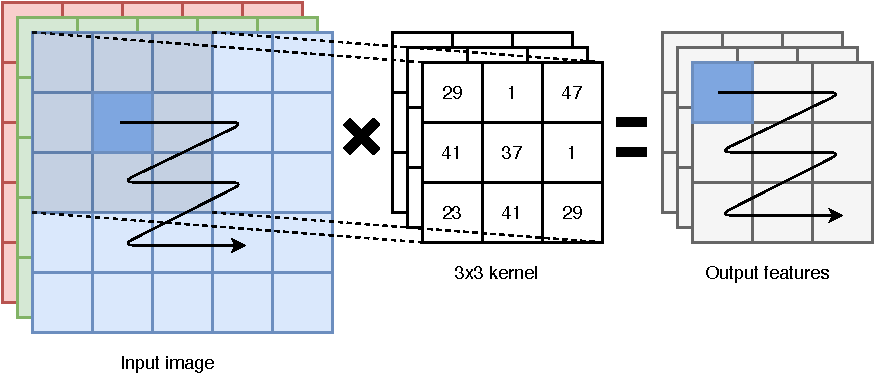
\includegraphics[width=0.9\textwidth]{conv}
	\caption{Convolutional filtering operation with a 3 channel RGB image and 3x3 kernel}
	\label{fig:conv}
\end{figure}

In Figure \ref{fig:conv} a convolutional filtering operation over an image is illustrated. The matrix kernel is moved in a row by row pattern and is multiplied by a patch of the image to get a value for the output cell.

In order to form a deep neural network multiple filtering operations are chained sequentially with nonlinear activation functions between them. A deep neural network usually consists of many such layers of filtering operations and activation functions. This concept is illustrated in Figure \ref{fig:deep}.

\begin{figure}[H]
	\centering
	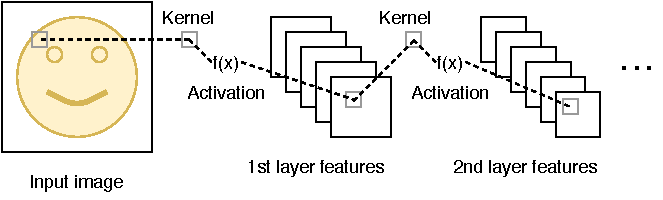
\includegraphics[width=0.8\textwidth]{deep}
	\caption{Multiple layers chained with each other to form a deep network}.
	\label{fig:deep}
\end{figure}

The activation functions need to be differentiable because the derivatives are used in the learning process. Some common nonlinear activation functions are shown in Figure \ref{fig:activation}.

\begin{figure}[H]
	\centering
	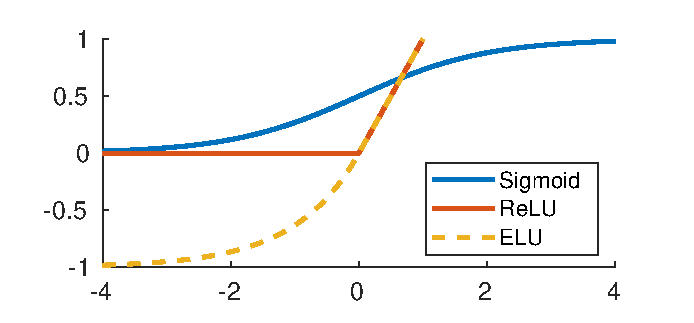
\includegraphics[width=0.6\textwidth]{activation}
	\caption{A few common nonlinear activation functions.}
	\label{fig:activation}
\end{figure}

The features in the deep neural networks are used to formulate a loss function. The loss defines an objective that we want the network to learn. This means that the process of learning becomes a task of updating the filter kernels in such a way that the loss function is minimized. If the loss function is decreasing during the training process it means that the network is learning. It is crucial that the loss function describes the problem accurately, otherwise the network will not learn the correct behavior. The weights in the network are updated using a method called back propagation. The algorithm computes the gradient of the loss function with respect to the weights in the network for a single input example from the training data using the derivative chain rule, which can be done very efficiently. Updating the weights to minimize the loss function can then be done using gradient decent. As the network is fed with more input examples from the training data, the network slowly learns the correct weights that minimizes the loss function as desired.





\section{Unsupervised learning}
\chapter{Related work}\label{cha:relatedwork}


In this chapter some of the important contributions of previous research papers are summarized. Firstly a list of papers in the field of unsupervised depth and ego motion prediction is presented. Secondly a paper on unsupervised feature point prediction. Thirdly a paper on unsupervised geometric consensus maximization that was implemented in this thesis. Finally a paper on combining depth and feature point prediction, albeit using classical consensus maximization that is not learned by a neural network.

\section{Unsupervised depth and ego motion prediction}
\label{sec:rldepth}

All the papers in this section are discussed in the order of publication to show a timeline of progress in the field of depth and ego motion prediction.

%\section{Unsupervised Monocular Depth Estimation with Left-Right Consistency}
%\label{sec:relwork:leftright}

In this paper\cite{leftright} the authors present MonoDepth, with an implementation available in Tensorflow on github. In this work the depth is predicted using an encoder-decoder type network, but the relative motion between frames is not estimated at all. The KITTI dataset provides stereo image pairs which are used during training, and the relative transformation between the left and right cameras is known. Using only the left image as input to the network both disparity maps for the left and right images are predicted. The two disparity maps are used to project the left image into the view of the right image and vice versa. This can be seen as a precursor to the papers discussed later which uses only a monocular camera and several frames over time to train a depth predicting network and pose predicting network jointly. The L1 norm of the per pixel photometric error as well as \abbrSSIM\cite{ssim} are computed and added to the loss. An additional loss term encourages the left disparity to be equal to the right disparity projected into the left camera viewpoint. Because the photometric error does not work well on low textured regions an edge aware smoothess term is added to propagate the depth values from nearby areas in the disparity map. The method produces metrically accurate results because the baseline and focal length of the cameras are known.

%\section{Unsupervised Learning of Depth and Ego-Motion from Video}
%\label{sec:relwork:unego}

In this paper\cite{sfmlearner} the authors present SfMLearner with an official implementation in Tensorflow on github. Contrary to the previous paper\cite{leftright} only a monocular sequence of images from the KITTI dataset is used during training. In the stereo case the relative pose between the left and right cameras was known, but with this monocular dataset the pose between subsequent frames is unknown. The authors train a pose predicting and depth predicting network simultaneously with a joint loss function to solve this problem. During training 3 subsequent frames are considered at a time. The frame $I_{t-1}$ and frame $I_{t+1}$ are called the source frames and the frame $I_t$ is called the target frame. The target frame is input to the depth network which estimates a disparity map. The two source frames are fed through a pose estimating network one after each other together with the target frame to find the relative transformations $T_{t	\rightarrow t-1}$ and $T_{t	\rightarrow t+1}$. The authors add an explainability mask to the photometric error term to account for errors in the model. The view synthesis formulation implicitly assumes that the scene does not contain moving objects, that there are no occlusions between the target and source frames, and that the surfaces are Lambertian so that the photo-consistency error of \abbrRGB values is meaningful. In order to predict the explainability mask an additional \abbrCNN is used. The network has no explicit supervisory signal but is encouraged to be non-zero with an regularization term using a cross-entropy loss with a constant label 1 at each pixel location. This makes the network minimize the view synthesis objective but is allowed some slack due to factors not considered by the model. In later work it was shown that the explainability mask does not help to improve results that much and is often ignored. To tackle the problem with textured areas and non Lambertian surfaces, a smoothess term is used. An edge aware smoothess term was not used like in previous work\cite{leftright} but a penalty on the second order gradient of the depth map was used instead. This unfortunately makes edges very fuzzy in the results compared to using the edge aware smoothness loss.

%\section{SuperDepth: Self-Supervised, Super-Resolved Monocular Depth Estimation}

% TA BORT?
In this paper\cite{superdepth} the authors train a depth estimating network on only stereo image pairs. After the depth predicting network has been trained the pose network from \cite{sfmlearner} is trained, using results from the already trained depth predicting network. This means that the depth and pose networks are not trained with a joint loss function but are instead trained separately. The main contributions from this paper is a new subpixel-convolution operation that super-resolve disparities from their low-resolution outputs, thereby replacing the up-sampling layers typically used in the disparity decoder network. The method additionally uses differentiable flip-augmentation to remove edge artifacts on the left and right edges of the depth map seen in previous work using stereo image pairs during training. To handle occluded pixels between the left and right images an occulsion regularization loss term is added to encourage background depths (low disparaty).

%\section{3D Packing for Self-Supervised Monocular Depth Estimation}

% TA BORT?
In this paper\cite{packnet} the authors present PacknetSfM. The main contribution is a new network architecture with packing and unpacking blocks replacing down and up sampling. The new packing blocks use space to depth transformations and 3d convolutions. The authors claim that the new packing and unpacking blocks are better at perserving resolution than standard down and upsampling. As the method is not adopted in later work, it is unclear if the new packing and unpacking approach is effective. The second contribution is a loss on the camera velocity that makes it possible for the monocular depth estimation to be metrically accurate. The velocity of the car is assumed to be known in the training dataset. The third contribution is a mask on pixels that do not change between frames. These pixels are assumed to be part of objects that are stationary with respect to the camera. Such pixels can occur for example if the car dashboard is visible in a frame, or other vehicles are moving at a similar speed nearby.

%\section{Digging Into Self-Supervised Monocular Depth Estimation}

In this paper\cite{monodepth2} the authors present MonoDepth2. They propose mainly two contributions. Firstly, instead of taking the average of the reprojection errors from all source frames given a target frame they use the minimum. This makes it so that if a feature is occluded in one source image but not in the other the errors will not be averaged together but instead the error from the source frame that is not occluded will be used. Secondly, instead of calculating the loss for each depth scale in the decoder, all the depth maps are up-sampled to the original target image size when computing the loss. This way a single pixel in the low resolution layer of the decoder will predict the depth of a patch of pixels in the originally sized input image.

\section{Unsupervised keypoint prediction}
%\section{UnsuperPoint: End-To-End Unsupervised Interest Point Detector and Descriptor}

Collecting ground truth data to train a neural network for keypoint detection is cumbersome. What constitutes a keypoint is hard to define clearly and consistently for a human annotator.

SuperPoint\cite{superpoint} uses a unsupervised approach to learn prediction of points and their descriptors. The network is first trained on  a synthetic dataset of simple geometric shapes. The pseudo ground truth points are defined as the corners and junctions in the synthetic images. This pre-trained network is then trained on "real" images in a siemese network setup using a method they call homographic adaptation. The two siamese siblings are fed images transformed by random but known homographies and the output from the networks are compared in the loss function. The output of SuperPoint is a heatmap where each pixel describes the "point-ness" of that pixel, and a descriptor map. To keep the model fast both the point and descriptor maps are predicted semi-dense grid,
one cell for each 8 pixel patch. The maps are up-sampled to the original image size using bicubic interpolation, and the descriptors are normalized.

UnsuperPoint\cite{unsuperpoint} is heavily inspired by SuperPoint but does not need to be pre-trained on a synthetic dataset, instead it is trained in one round of training on real images. It uses a similar method of using siamese networks and homography adaptation during traning, but the output from the network is different. The network uses regression of actual point position coordinates instead of a heat map, incorporates non-maximum suppression, predicts scores for each keypoint and a sparse descriptor map that is sampled and interpolated using the point positions.

\section{Unsupervised geometric consensus maximization}
%\section{Unsupervised Learning of Consensus Maximization for 3D Vision Problems}

Consensus maximization is an important strategy in 3D vision problems for robust geometric model estimation from measurements including outliers. The classical method of \textit{Random Sampling and Consensus}, or RANSAC\cite{ransac} for short, is widely popular with great success. But replicating the same generic behavior using supervised training of neural networks has proven difficult. Unsupervised methods have a huge potential to generalize to any unseen data distribution and are in this context very desirable. This paper\cite{consensus} introduces just such an unsupervised method of consensus maximization for 3D vision problems. Using the relationship between the set of inliers, and the subspace of polynomials representing the space of target transformations a model fitting cost can be can be defined without knowing the specific parameters of the geometric transformation. During learning the loss is defined in a way to learn the largest set of inliers with a low model fitting cost. The geometric model parameters can then be extracted from the polynomials after network has learnt to distinguish inliers and outliers.

\section{Combined depth and feature point detection}

In a paper\cite{keypointdepth} the authors combines the previously discussed MonoDepth2\cite{monodepth2} for depth prediction, but also adds keypoint learning from SuperPoint\cite{superpoint} into the pipeline. The researchers train the depth, keypoint and pose estimating networks jointly, making them benifit from each other and achieve state of the art performance.  However, the step that finds possible outlier keypoints, is not differentiable and is not trained jointy with the depth and keypoint networks. The step that calculates the model parameters of the geometric relationship between corresponding keypoints also requires an initial guess that is not differentiable.


\chapter{Method}\label{cha:method}

This chapter describes the methods used to answer the research questions. The first question relates to the datasets used during training and testing of the networks. The second question relates to the performance benefits of applying specific techniques from previous research in unsupervised monocular depth and ego motion prediction.

To begin with, the chapter summarizes which datasets were used in this thesis and how the choice relates to the first research question. Following that, an explanation is given, of which specific techniques for monocular depth prediction are evaluated in the results chapter, and the method used to combine them. Lastly a detailed description of all the error and accuracy metrics that are presented in the results chapter. A good understanding of what the metrics imply is needed to answer both research questions.

\section{Datasets}

The neural networks are trained and evaluated on images from 2 different datasets, KITTI\cite{kitti} and Lyft\cite{lyft2019}. Both datasets are preprocessed to remove frames where the camera is not moving. This is important because if there is no movement between frames then no depth information can be inferred during training when using monoscopic data. In the Kitti dataset the images from the left and right camera are treated as separate image sequences to yield more training data. The images are resized to $128\times 416$ pixels, and the intrinsic camera matrix is updated accordingly.

\subsection{Sequence datasets}

To train the networks used for depth and ego motion prediction the images from Kitti and Lyft at loaded in triplets of subsequent frames in a sequence.

The lidar data from Kitti and Lyft is converted to a sparse depth map, together with the ground truth ego motion. This data is only used during testing, not during training.
adjacent
\begin{figure}[H]
	\centering
	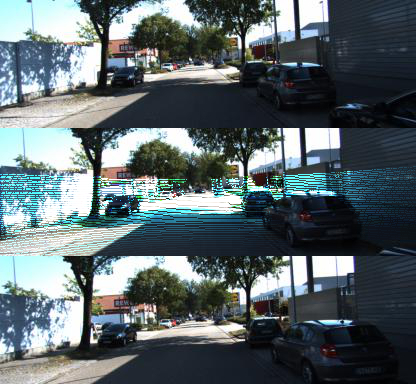
\includegraphics[width=0.5\textwidth]{sequencedataset}
	\caption{The dataloader loads 3 subsequent frames in a sequence. The figure shows from top to bottom 3 frames from Kitti, $I_{t-1}$, $I_t$, $I_{t+1}$ with the sparse depth map overlayed on frame $I_t$.}
	\label{fig:sequencedataset}
\end{figure}

Kitti contains 124 sequences, and Lyft contains 148 sequences. For each dataset the sequences are split, approximately 90\% is used for training and 10\% for testing.

\begin{table}[H]
	\centering
	\begin{tabular}{ |c|c|c|c|c| } 
		\hline
		&\multicolumn{2}{c|}{Sequences / Samples} \\ 
		\hline
		& Train & Test \\ 
		\hline
		Kitti & 110 / 16542 & 12 / 11349 \\ 
		\hline
		Lyft & 134 / 3759 & 14 / 1735 \\ 
		\hline
	\end{tabular}
	\caption{The training sequences are split into a training set and a testing set.}
	\label{table:datasets}
\end{table}

\subsection{Homographic adaptation dataset}

To train the network that predicts keypoints, images are read one by one from the Kitti or Lyft datasets. The image is fed trough two branches, in branch A the image is not modified, and in branch B the image is transformed by a random homography (Figure \ref{fig:unsuperpointloss}). The authors of UnsuperPoint refer to this technique as homographic adaptation.

How to generate the random homography used during training is not described in the UnsuperPoint paper, but is an important part of the method. The method used in this thesis generates random homographies from 5 parameters $\alpha_{rotation}$, $\alpha_{translation}$, $\alpha_{scale}$, $\alpha_{sheer}$ and $\alpha_{perspective}$. The parameters controls the maximum transformation for each aspect of an homography. The final homographgy is constructed from parts as follows.

\[
H = H_{affine} H_{sheer} H_{perspective}
\]

Assume $u_n \sim U(-1,1)$ are random uniform variables in the range -1 to 1.

\[
H_{affine} = 
\begin{pmatrix}
\cos(r)*s & -\sin(r) & t_x \\
\sin(r)& \cos(r)*s & t_y \\
0 & 0 & 1 \\
\end{pmatrix}
, \text{with}
\begin{cases}
r=u_1*\alpha_{rotation} \\
s=u_2*\alpha_{scale}+1 \\
t_x=u_3*\alpha_{translation} \\
t_y=u_4*\alpha_{translation} \\
\end{cases}
\]

\[
H_{sheer} = 
\begin{pmatrix}
1 & s & 0 \\
s & 1 & 0 \\
0 & 0 & 1 \\
\end{pmatrix}
, \text{with}
\ s=u_5*\alpha_{sheer} \\
\]

\[
H_{perspective} = 
\begin{pmatrix}
1 & 0 & 0 \\
0 & 1 & 0 \\
p & p & 1 \\
\end{pmatrix}
, \text{with}
\ p=u_6*\alpha_{perspective} \\
\]

The output from the network is used together with the random but known homography to formulate the loss function.

TODO: Illustration of training data for consensus maximization



\section{Comparing techniques for depth and egomotion prediction}

To answer the second research question, a system of enabling and disabling terms in the loss function was implemented. The effect on performance for a few particular loss terms discussed in the related work was measured. By enabling a selection of loss terms (Table \ref{table:configurations}) in different experiments (Table \ref{table:experiments})  their respective contribution to the results can be observed. The command line options to the program used to train the models are listed in Table \ref{table:cli}. An deeper explanation of these techniques can be found in chapter \ref{cha:implementation}.

\begin{table}[H]
	\centering
	\begin{tabular}{ |l|l|p{65mm}| }
		\hline
		Command line option & Name & Description \\
		\hline
		\texttt{-{}-net} & Net & Network architecture (SfMLearner or Monodepth2). \\
		\hline
		\texttt{-{}-dataset} & DS & Dataset for training (Kitti or Lyft). \\
		\hline
		\texttt{-{}-explain-mask} & Expl & Filter pixels using explainability mask (section \ref{sec:modellimit}) \\
		\hline
		\texttt{-{}-stationary-mask} & Stat & Filter pixels using stationary pixels mask (section \ref{sec:modellimit}) \\
		\hline
		\texttt{-{}-ssim} & SSIM & Use SSIM in combination with L1 in the photometric error term (section \ref{sec:loss}). \\
		\hline
		\texttt{-{}-depth-map-norm} & Norm & Normalize the depth map (section \ref{sec:normalization}) \\
		\hline
		\texttt{-{}-edge-aware} & Edge & Use edge aware depth smoothness loss term (section \ref{sec:loss}) \\
		\hline
		\texttt{-{}-upscale} & US & Use up-scaling of the smaller depth maps in the decoder (section \ref{sec:upscale}). \\
		\hline
		\texttt{-{}-min-loss} & Comb & Combine loss from $t-1$ and $t+1$ with \texttt{min} instead of \texttt{avg} (section \ref{sec:occlusion}). \\
		\hline
	\end{tabular}
	\caption{A list of command line option for the PyTorch training script. The column Name contains the naming used for each technique when they are used to form the configurations in Table \ref{table:configurations} in chapter \ref{cha:results} Results.}
	\label{table:cli}
\end{table}

\section{Evaluation metrics}

This section describes the metrics used to evaluate depth, ego motion, feature point and consensus maximization predictions. These specific metrics where chosen because they are also used in the related works in this field, which makes the results comparable to other papers.

\subsection{Depth error and accuracy metrics}
\label{sec:depthmetrics}

The depth error and accuracy metrics are sparse and only calculated for the pixels of which there exists a ground truth laser measurement in the dataset. The values are averaged over all laser measurements and frames in the test split of the dataset. An error of 0 and an accuracy of 1 is optimal, but can never be achieved in practice.

The depth is predicted relative to an unknown scale, and the ground truth is measured in meters. To alleviate this issue the depth predictions are scaled so that their median is the same as the median of the ground truth for each frame. This does not guarantee that the unit of the predictions is meters, but at least it makes the scales somewhat similar.

The error metrics used in the results chapter are referred to as \textit{Abs Rel}, \textit{Sq Rel}, \textit{RMSE} and \textit{RMSLE}.

The \textit{Abs Rel} error is based on \textit{MAE} which is the mean of the absolute errors which means that it has the same unit as the errors, and is conceptually quite easy to interpret.

\[
\textrm{MAE}=\frac{\sum^N_{n=1}{|y_n-\hat{y}_n|}}{N}
\]

Because the depth from the neural network is without unit and only predicted relative to an unknown scale, a variation on the \textit{MSE} metric called \textit{Abs Rel} is used.

\[
\textrm{Abs Rel}=\frac{\sum^N_{n=1}{\frac{|y_n-\hat{y}_n|}{y_n}}}{N}
\]

The \textit{MSE} metric is the mean of squared errors, for an unbiased estimator it represents the variance of the errors. 

\[
\textrm{MSE}=\frac{\sum^N_{n=1}{(y_n-\hat{y}_n)^2}}{N}
\]

Once again, because the depth is predicted relative to an unknown scale a variation on \textit{MSE} called \textit{Sq Rel} is used instead.

\[
\textrm{Sq Rel}=\frac{\sum^N_{n=1}{\frac{(y_n-\hat{y}_n)^2}{y_n}}}{N}
\]

The \textit{RMSE} metric is the square root of the mean of squared errors. For an unbiased estimator it represents the standard deviation of the errors. Because the errors are squared in the \textit{RMSE} metric it is more sensitive to outliers that for example \textit{MSE}.

\[
\textrm{RMSE}=\sqrt{\frac{\sum^N_{n=1}{(y_n-\hat{y}_n)^2}}{N}}
\]

The \textit{RMSLE} metric is similar to \textit{RMSE} but is useful because it penalizes large errors less when both the actual and predicted values are large.

\[
\textrm{RMSLE}=\sqrt{\frac{\sum^N_{n=1}{(\log{y_n}-\log{\hat{y}_n)}^2}}{N}}
\]

To measure the depth accuracy, in the range from 0 to 1, the following metric is used.

\[
a_{\gamma} = \frac{\sum^N_{n=1}{(\max(\frac{y_n}{\hat{y}_n}, \frac{\hat{y}_n}{y_n}) < \gamma)}}{N},\textrm{ for }\gamma \in \{1.25, 1.25^2, 1.25^3\}
\]

This should be interpreted as the ratio of predictions that is within the ratio of $ \gamma $ relative to the ground truth.

\subsection{Camera ego motion error metric}
\label{sec:egometric}

The error of the camera motion predictions are measured using \textit{RMSE}. But instead of taking the mean error over all poses in a sequence, the alignment error is calculated part wise over a track length of only 5 poses. The final error is presented as the mean \textit{RMSE} of all parts. Each track part from the prediction is transformed to have its first pose coincide with the ground truth in a common origo. This is done so that the first pose in the track part of both the prediction and ground truth is the identity matrix $I \in \mathbb{R}^{4\times 4}$. Because the ego motion is predicted relative to an unknown scale and the ground truth is in meters, we scale each predicted track part to have similar scale to the ground truth track part.

\subsection{Keypoint error and score metrics}\label{sec:keypointmetrics}

The unsupervised keypoint network was compared with the ORB feature detector from OpenCV. To messure the performance differences 3 different metrics where used, repeatability score (RS), localization error (LE), matching score (MS), and matching ratio (MR).

Before any of the metrics are calculated the points are first filtered to remove all points within 10px of the edges. This is done to not include detections where the black background meets the border of the transformed image.

\begin{figure}[H]
	\centering
	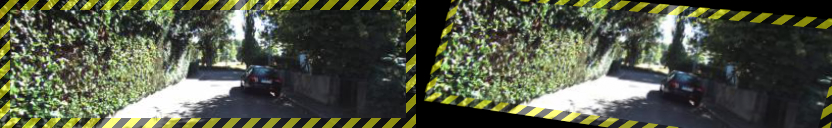
\includegraphics[width=1.0\textwidth]{remove-edges}
	\caption{The black and yellow stripes illustrates the are where keypoint detections are filtered out and discarded.}
	\label{fig:remove-edges}
\end{figure}

To calculate the set of ground truth correspondences, the points in the left image is transformed by the known homography $H$. A point in the left image is corresponding with a point in the right image if they are their closes neighbor and the distance is less than 3px after the transformation. This set of ground truth correspondences is used in all metrics. If the images contain a different amount of points, the largest set of possible correspondences that could have been found is $N_{tot} = \min(N_{left}, N_{right})$. The number of ground truth correspondences (closer than 3px) is $N_{gt} \le N_{tot}$.

Repeatability score (RS) is a measure on how good a method is at repeatedly highlighting the same physical features in the scene but in different images. Because the keypoint algorithm is only fed one image at the time, it is important that there is consistency in what physical features are selected in the image, otherwise their will be very few actual correspondences.

\[
RS = \frac{N_{gt}}{N_{tot}} 
\]

Localization error (LE) is a measure of the average distance error between the ground truth corresponding points. It will always be less than 3px because that is our definition of a correspondence, but the ideal is 0px.


Matching score (MS) is a measure on how many keypoints are matched correctly based on their descriptors. The set of points that are both ground truth correspondences and are corresponding based on their predicted descriptors are said to be correctly matched. The number of correctly matched points are $N_{correct}$.

\[
MS=\frac{N_{correct}}{N_{tot}}
\]

Matching ratio (MR) is very similar to matching score. To get a high MS requires both good repeatability and good descriptors, but getting an MR requires only good descriptors.

\[
MR=\frac{N_{correct}}{N_{gt}}
\]

\subsection{Consensus maximization performance metrics}\label{sec:consensusmetrics}

The unsupervised consensus maximization network that predicts homographies was compared with the \textit{findHomography()} function in OpenCV.

The homography error (HE) is calculated as the average distance between the corners of the image when it is transformed by the estimated homography compared to the ground truth homography.

\begin{figure}[H]
	\centering
	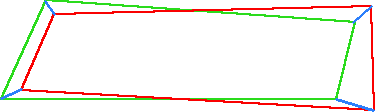
\includegraphics[width=0.5\textwidth]{he}
	\caption{The corners of the image transformed by the ground truth homography and the predicted homography is shown in green and red respectively. The homography error (HE) is calculated as the average of the distances shown in blue.}
	\label{fig:he}
\end{figure}

In order to evaluate the methods ability to distinguish inliers and outliers among the points, a confusion matrix is used. The ground truth set of inliers, or ideal, is the same as the one calculated in section \ref{sec:keypointmetrics}. The confusion matrix shows the ratio of true positives, true negatives, false positives and false negatives in the inlier classifications. The confusion matrix is normalized on the axis of ground truth so that the sum of true positives and false negatives adds up to 1, and the sum of the false positives and true negatives also adds up to one.

\begin{table}[H]
	\centering
	\begin{tabular}{l|l|c|c|c}
		\multicolumn{2}{c}{}&\multicolumn{2}{c}{Predicted}&\\
		\cline{3-4}
		\multicolumn{2}{c|}{}&Inlier&Outlier&\multicolumn{1}{c}{Total}\\
		\cline{2-4}
		\multirow{2}{*}{Actual}& Inlier & TP & FN & $TP+FN=1$\\
		\cline{2-4}
		& Outlier & FP & TN & $FP+TN=1$\\
		\cline{2-4}
		\multicolumn{1}{c}{} & \multicolumn{1}{c}{Total} & \multicolumn{1}{c}{$TP+FP$} & \multicolumn{    1}{c}{$FN+TN$} & \multicolumn{1}{c}{$2$}\\
	\end{tabular}
	\caption{Structure of confusion matrix for inlier classification.}
	\label{table:confusion}
\end{table}


\chapter{Implementation}\label{cha:implementation}

This chapters describes the implementation done in PyTorch for this thesis. The first part details the methods evaluated in depth and ego motion prediction, the second part describes the implementation of unsupervised keypoint prediction, and the last part describes how the consensus maximization network was implemented.



\subsection{Architectures for depth and ego motion CNNs}

In order to predict depth and motion from monocular images two different CNN architectures are examined. Both are encoder-decoder type architectures, and their general layout is illustrated in Figure \ref{fig:net}.

The first architecture is referred to as SfMlearner\cite{sfmlearner}, and uses a DispNet\cite{dispnet} architecture is used to predict depth maps at four different scales.

The second architecture is referred to as Monodepth2\cite{monodepth2}, and uses a ResNet18 architecture instead of a DispNet architecture to predict depth estimates. This architecture is a smaller resulting in faster training and evaluation.

Both SfMlearner and Monodepth2 uses a separate network to predict poses between frames. The pose network has a ResNet18\cite{resnet} architecture, but the decoder is modified to predict pose updates in an euler angle axis representation.

\begin{figure}[H]
	\centering
	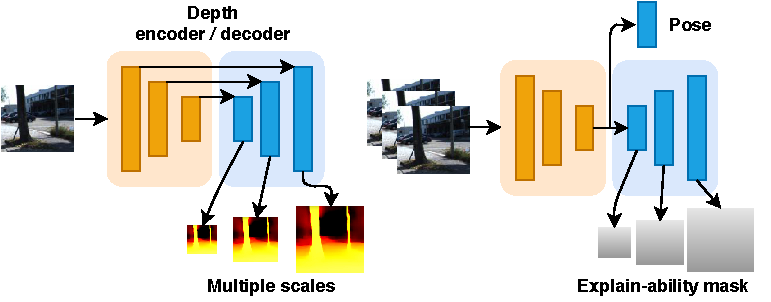
\includegraphics[width=1.0\textwidth]{net}
	\caption{High level diagram of the network architectures used for depth and ego motion prediction. The layers from the depth encoder are concatenated into the layers of the decoder. Depth maps are computed at multiple scales in the decoder and are all used in the loss function. A separate network that takes as input 3 subsequent frames predicts the poses $\textbf{T}_{t\rightarrow t-1}$ and $\textbf{T}_{t\rightarrow t+1}$ between the target and nearby reference frames. The pose network shares encoder with the explain-ability mask predicting network (section \ref{sec:modellimit}).}
	\label{fig:net}
\end{figure}

\subsection{Differentiable depth image warping}
\label{sec:diffwarp}

The core component of unsupervised depth learning is the differentiable depth image warp operation in the loss function of the CNN networks. Given the intrinsic camera matrix:

\begin{equation}
\textbf{K} = 
\begin{pmatrix}
f_\mathrm{x} & s & x_0 \\
0 & f_\mathrm{y} & y_0 \\
0 & 0   & 1
\end{pmatrix}
\end{equation}

And the predicted depth $ D_t(p_t) $ of pixel $ p_t $ of the target (current) frame. And the transform $ T_{t \rightarrow s} $ from the target to source (next/previous) frame:

\begin{equation}
\textbf{T}_{t \rightarrow s} =
\begin{pmatrix}
\textbf{R} & \textbf{t} \\
0 & 1
\end{pmatrix}
\end{equation}

The position of the target pixel $ p_t $ in the source image $ p_s $ can be calculated in homogeneous coordinates as:

\begin{equation}
\textbf{p}_s \sim 
\begin{pmatrix}
\textbf{K}  & \textbf{0} \\
\end{pmatrix}
\textbf{T}_{t \rightarrow s} \textbf{D}_t(\textbf{p}_t) \textbf{K}^{-1} \textbf{p}_t 
\end{equation}

The pixel position $ p_s $ is however continuous and in order to sample the discrete source image $ \textbf{I}_s $ a differentiable bilinear sampling method is used. The method is described in \textit{spatial transformer networks}\cite{spatialtransformernetworks} and works by interpolating the neighbouring 4 pixels values (top-left, bottom-right) by the distance to the the continuous sampling point $ p_t $. This process is illustrated in Figure \ref{fig:warp}.


\begin{figure}[H]
	\centering
	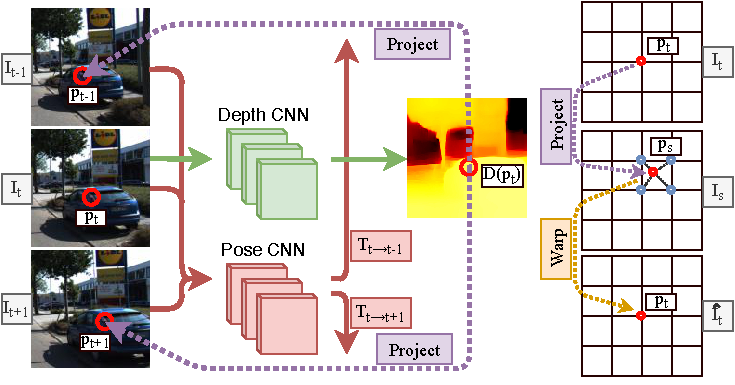
\includegraphics[width=1.0\textwidth]{warp}
	\caption{The \abbrCNN predicts the depth map $\textbf{D}$ of the target image $\textbf{I}_t$, and also the relative movement, $\textbf{T}_{t\rightarrow t-1}, \textbf{T}_{t\rightarrow t+1}$ between the target image and the source images. Each pixel $p_t$ in the target image is projected onto a position in the source images which are sampled using bilinear interpolation. This should recreate the appearance of the target image but with pixels sampled from the source image. An appearance similarity metric between the original target image and the recreated target images can be used as the loss function for the \abbrCNN to learn to accurately predict correct depth and movement.}
	\label{fig:warp}
\end{figure}

%TODO: Insert examples of warped/recreated and diff images between target and recreated images.....


\subsection{Loss functions}
\label{sec:loss}

In order to learn the objective of depth and ego motion prediction, different combinations of the following loss terms where evaluated.

To measure the similarity of the target image $\textbf{I}_t$ and the reconstructed image $\hat{\textbf{I}}_t$ a photometric loss term defined as the mean of the absolute value of the difference of pixel intensities of the two images was used.

\begin{equation}
\mathcal{L}_p(\textbf{I}_t, \hat{\textbf{I}}_t)=\mean(|\textbf{I}_t - \hat{\textbf{I}}_t|)
\end{equation}

Another photometric loss term evaluated in this thesis is based on structured similarity, referred to as SSIM\cite{ssim}. It was originally developed to measure the quality of digital television, comparing a compressed digital image to the original distortion-free image.

\begin{equation}
\mathcal{L}_{ssim}(\textbf{I}_t, \hat{\textbf{I}}_t)=\mean(\clamp(\textbf{0},\textbf{1},\dfrac{\textbf{1}-\SSIM(\textbf{I}_t, \hat{\textbf{I}}_t)}{2}))
\end{equation}
\begin{equation}
\SSIM(x,y)=\frac{(2\mu_x\mu_y+C_1)(2\sigma_{xy}+C_2)}{(\mu_x^2+\mu_y^2+C_1)(\sigma_x^2+\sigma_y^2+C_2)}
\end{equation}

with $C_1=1e-4$ and $C_2=9e-4$. To compute the per-patch mean $\mu_x$ and standard deviation $\sigma_x$, a 1 pixel reflection padding was first used on the edges of the input images and then a $3\times3$ average pool filter with stride 1 was used to get the mean. Then $ \sigma_x=\mu_{x^2}-\mu_x^2 $.

The two above mentioned photometric loss terms can also be combined and balanced using $ \mathcal{L}_{ps}(\textbf{I}_t, \hat{\textbf{I}}_s) = \alpha \mathcal{L}_{ssim} + (1-\alpha) \mathcal{L}_p $. In the experiments of this thesis $\alpha=0.85$ was used, which is the same value used in the original Monodepth2 paper. As the network learns over time to predict more accurate depth and ego motion, the reconstruction loss will decrease. The loss per individual pixel is illustrated in Figure \ref{fig:diff}, which shows the loss from the same sample but after 1 and 30 epochs of training respectively.

\begin{figure}[H]
	\centering
	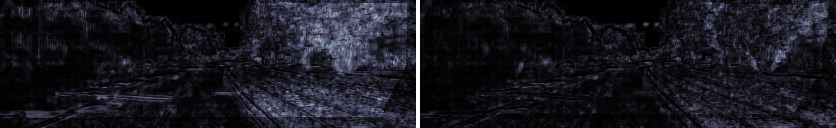
\includegraphics[width=1.0\textwidth]{diff}
	\caption{The images illustrates the photometric reconstruction loss $ \mathcal{L}_{ps} $ for each pixel in a reconstructed image for the same frame but after different length of training. The left image shows the loss after 1 epoch of training and the right image shows the loss after 30 epochs. The reconstruction loss should decrease during training as the network learns to predict better depth maps, which is what we see.}
	\label{fig:diff}
\end{figure}

To propagate the depth from textured regions to regions of uniform color a depth smoothness loss term is used. The first alternative is a loss on the second derivative of the depth intensities. This loss term will discourage the network to predict fluctuating depth values in regions of uniform color such as the pavement, that should be smooth. The drawback of this technique is that changes in depth values are penalized equally in regions where there are a lot of detail that therefore could be lost in the depth map.

\begin{equation}
\mathcal{L}_{smooth}(\textbf{D}_t)=\mean(|\delta_x^2 \textbf{D}_t|+|\delta_y^2 \textbf{D}_t|)
\end{equation}

The second alternative investigated was an edge aware smoothness loss that weights the first order derivative of the depth map with the exponential of the first derivative of the pixel intensities. This method allows large changes in depth near sharp features in the image but penelizes changes in depth in smooth regions, see Figure \ref{fig:edge}. The method showed great promise, resulting in sharper edges because the smoothness term is weighted to mostly affect areas with small photometric derivative.

\begin{equation}
\mathcal{L}_{edge}(\textbf{D}_t)=\mean(|\delta_x \textbf{D}_t|e^{-|\delta_x \textbf{I}_t|} + |\delta_y \textbf{D}_t|e^{-|\delta_y \textbf{I}_t|})
\end{equation}

\begin{figure}[H]
	\centering
	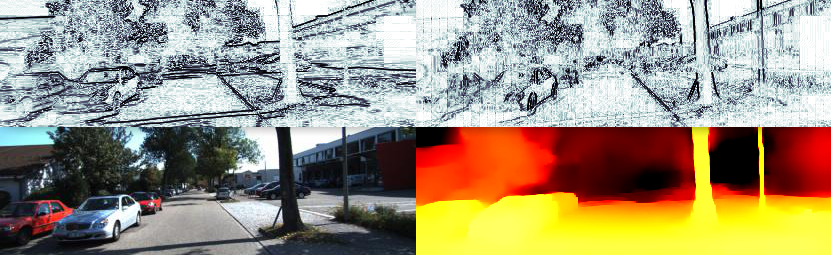
\includegraphics[width=0.9\textwidth]{edge}
	\caption{The top row of images illustrates the edge weighting terms $e^{-|\delta_y \textbf{I}_t|}$ and $e^{-|\delta_x \textbf{I}_t|}$ respectively. The weight is near 0 at the edges of tree trunks and near 1 on the pavement. This will preserve the details in the depth map around trees but keep the pavement smooth.}
	\label{fig:edge}
\end{figure}

\subsection{Depth map normalization}\label{sec:normalization}

The predicted depth is scale invariant which can make it difficult to balance the loss terms with the correct weights. To alleviate this is issue the depth map can be normalized before it is used in the loss.

\begin{equation}
\hat{\textbf{D}_t} = \frac{\textbf{D}_t}{\median(\textbf{D}_t)} 
\end{equation}

\subsection{Depth map up-scaling}\label{sec:upscale}

The smaller depth maps in the depth decoder of the network are all used in the loss. Early work in this area down-scaled the target image to fit the size of the smaller depth maps when used in the loss function. But in MonoDepth2\cite{monodepth2} it was proposed to instead up-scale the depth maps to the original target image size, see Figure \ref{fig:upscale}.

\begin{figure}[H]
	\centering
	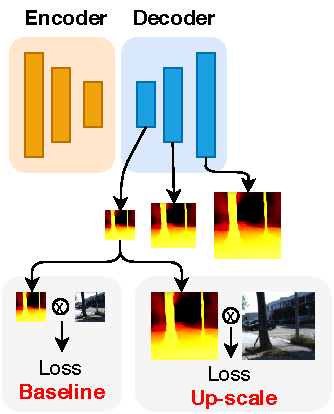
\includegraphics[width=0.3\textwidth]{upscale}
	\caption{The depth maps can optionally be up-scaled in the loss function.}
	\label{fig:upscale}
\end{figure}

\subsection{Handling occlusions}
\label{sec:occlusion}

\iffalse
\paragraph{Disparity loss} To encourage background depths (low disparities) in shadows of the depth map where occlusion has occurred a penalty on the disparity can be added $ \mathcal{L}_{o} =|d_t|. $
\fi

In the SfMLearner paper the photometric loss is calculated for the previous and next frames compared to the current in the sequence. The pixel wise average across the frames are then used. This causes problems if a pixel is for example occluded in the previous frame, but visible in the current and next frame. In this situation the average loss will be large even though a correct depth and transformation has been predicted, because of the occluded pixel. Instead Monodepth2 suggests to pick the minimum per pixel error over the frames which alleviates this issue, see Figure \ref{fig:min}. Both techniques where implemented in this thesis and compared in the experiments.

\begin{figure}[H]
	\centering
	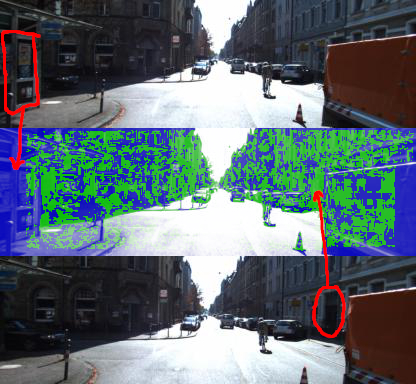
\includegraphics[width=0.5\textwidth]{min}
	\caption{By picking the per pixel minimum reprojection error the issue created by occluded pixels can be alleviated. The top image is the previous frame, the middle image is the current target frame and the bottom image is the next frame in the sequence. If the minimum reprojection error can be found in the previous frame then it is colored blue, if its from the next frame it is green. Because the door to the right is occluded by the orange truck in the previous frame, the reprojection loss from the next frame is used instead where the door is visible. The wall to the left is outside the boundaries of the next image, so the reprojection error from the previous frame is used instead.}
	\label{fig:min}
\end{figure}

\subsection{Handling model limitations}
\label{sec:modellimit}

In order to optimize using the photometric reprojecton error as the loss function two assumptions must hold. Firstly the scene must be static, meaning all objects in the scene must be still except the moving camera. Dynamic objects will cause problems. Secondly there must be photometric consistency between frames for the photometric error to make sense. This means that non lambertian surfaces, change in lighting, and change in exposure between frames will cause problems. Two different methods of dealing with this issue was implemented and evaluated in this thesis.

\paragraph{Explainability mask} The authors of \cite{sfmlearner} tackle this problem by having a CNN predict what pixels are valid to use in the photometric loss function, see Figure~\ref{fig:exp}. It shares the encoder of the pose predicting network but branches of into a different decoders which estimates a mask of the valid/explainable pixels. The loss function for the mask is the cross entropy loss compared to a mask filled with ones. The photometric loss function is augmented to include the explainability mask removing pixels that cannot be explained by the predicted depth and transformation. This encourages the mask to be filled with ones, but allows some slack due to pixels that can not be explained by the photometric loss.

\begin{figure}[H]
	\centering
	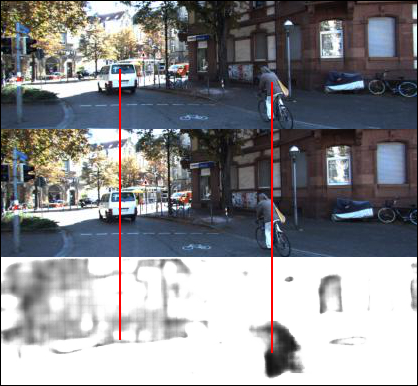
\includegraphics[width=0.5\textwidth]{exp}
	\caption{This is an image extracted from the experiments in this thesis. The top image is frame $\textbf{I}_t$ the middle image is frame $\textbf{I}_{t-1}$ and the last image is the explain-ability mask. It is visible that the network correctly predicts that the bicycle is not moving in relation to the camera, but it does not remove pixels from the white van as it should.}
	\label{fig:exp}
\end{figure}

\paragraph{Stationary pixels mask} The authors of \cite{monodepth2} introduced a mask to remove stationary pixels from the set of previous, current and next frame. This is done by creating a mask where the photometric error is smaller before applying the projection than after. This works because pixels from objects that have not moved in relation to the camera will of course have a small photometric loss without reprojection. This will remove pixels from the car dashboard and also nearby vehicles that are traveling at the same speed, see Figure \ref{fig:stat}.

\begin{figure}[H]
	\centering
	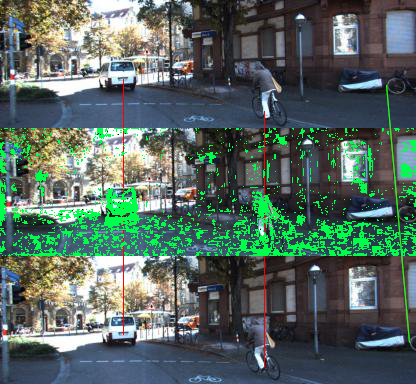
\includegraphics[width=0.5\textwidth]{stat}
	\caption{The black pixels in the image are the ones removed because their photometric error is smaller before warping the image using the depth map compared to after warping. The red horizontal lines on the van and bicyclist illustrates that they do not move with respect to the camera, and the green slanted line illustrates that the bike leaning on the wall is moving with respect to the camera. The mask successfully removes pixels on the van and bicyclist, but also removes some pixels on the pavement that should not be removed.}
	\label{fig:stat}
\end{figure}

\newpage
\section{Unsupervised keypoint learning}

In order to build a map it is useful to extract features, or keypoints, from images. Every keypoints should have a unique descriptor which can be used to identify it in the map which makes it possible to expand the map and also localize the camera. How to build a map and localize in it is out of scope for this thesis. This section will describe the usnupervised learning method implemented in this thesis, to extract keypoints from images.

The method evaluated in this thesis is based on the UnsuperPoint paper\cite{unsuperpoint}. The network architecture is illustrated in Figure \ref{fig:unsuperpoint}. The input image is fed into a shared backbone. The features from the backbone are then split into three different encoders that estimate the score, position and a descriptor for each keypoint. The network will estimate a keypoint in every $8\times 8$ patch of the image, but only the top $N$ keypoints sorted by score are used in the evaluation.

\begin{figure}[H]
	\centering
	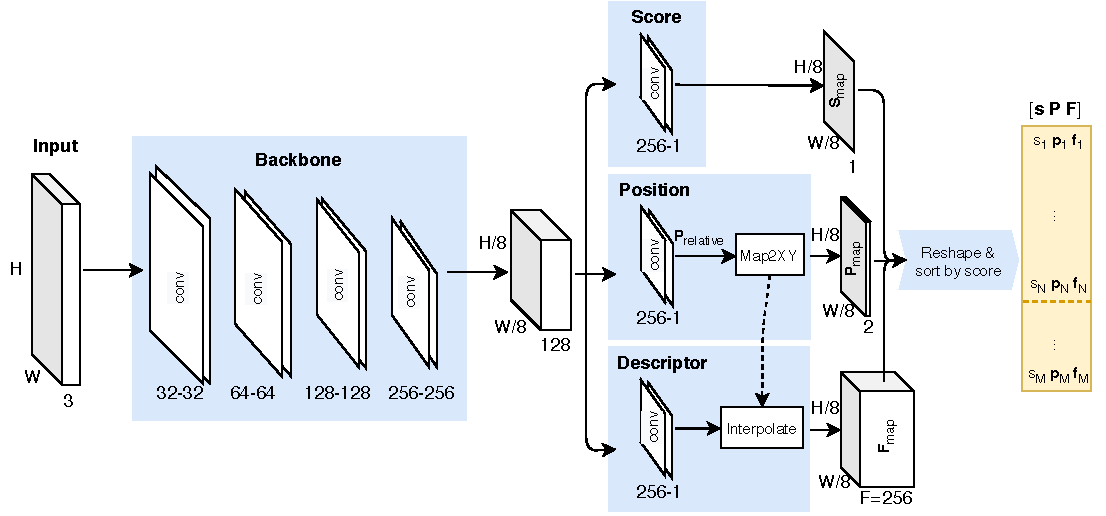
\includegraphics[width=1.0\textwidth]{unsuperpoint}
	\caption{The network has a common backbone and then splits into separate score, position and descriptor encoders. The output is reshaped and sorted by descending score.}
	\label{fig:unsuperpoint}
\end{figure}

The score encoder is terminated by a sigmoid function and outputs $S_{map}$, containing scores between 0 and 1 for each keypoint. The purpose of the scores are to rank the quality of the keypoints in all $8\times 8$px patches of the image and only pick the best ones. Typically patches in the sky and other non-textured areas will have keypoints with low scores.

The position encoder is also terminated by a sigmoid function and outputs $P_{relative}$ which is the relative position of the keypoint in each patch. In the Map2XY block in Figure \ref{fig:unsuperpoint} the relative positions are converted to absolute pixel positions to form $P_{map}$.

\[
P_{map,x}(r,c) = 8 * (c + P_{relative,x}(r,c))
\]
\[
P_{map,y}(r,c) = 8 * (r + P_{relative,y}(r,c))
\]

The descriptor encoder predicts a descriptor vector of length $256$ for each keypoint. The purpose of the descriptor is to find corresponding keypoints in different images. The encoder produces 1 descriptor vector for each $8\times 8$ patch in the image. This vector can be used directly as the keypoint descriptor and it works pretty well. Even better results can be achieved using the absolute keypoint positions to sample the values in the descriptor map with the same interpolation method used to do the warping in Figure \ref{fig:warp}.

$S_{map}$, $P_{map}$ and $F_{map}$ are reshaped into a vector $s$ of $M$ elements, an $M\times 2$ matrix $P$ and an $M\times 255$ matrix $F$, where $M=\frac{W}{8}*\frac{H}{8}=832$.

The network is trained in a siamese twin setup, where two duplicate networks that share weights are fed different inputs and the loss is formulated by comparing the output scores, positions and descriptors.

\begin{figure}[H]
	\centering
	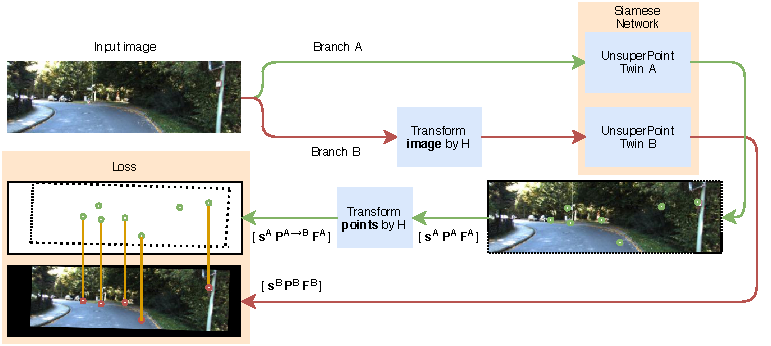
\includegraphics[width=1.0\textwidth]{unsuperpointloss}
	\caption{This figure illustrates the flow from input image to loss function. The image from branch A is fed directly into the UnsuperPoint network, while in branch B the image is first transformed by a random homography $H$. The keypoint positions from twin A are transformed by the same homography $H$ and the output from the two branches are compared in order to formulate the loss function.}
	\label{fig:unsuperpointloss}
\end{figure}

For each branch $b\in\{A,B\}$ the siamese networks output the reshaped matrices $s^b$, $P^b$ and $F^b$ which contain the scores, positions and descriptors of the $M$ points in each image.

\subsection{Loss function for keypoint learning}\label{sec:keypointloss}

To formulate the loss function the point correspondences between branch A and B need to be determined. The points in branch A are transformed such that $p_i^{A\rightarrow B}=Hp_i^A$. Then an $M^A\times M^B$ distance matrix $G$ is calculated from the pairwise distances between all points in each branch.

\[
G=[g_{ij}]_{M^A\times M^B}=\left[||p_i^{A\rightarrow B}-p_j^B||\right]_{M^A\times M^B}
\]

We define a point pair if point $i$ in branch A has a point $j$ as its closest neightbor in branch B, and if the distance $g_{ij}$ is less than 8px. With the point pairs defined the output matrices $s^b$, $P^b$ and $F^b$ can be redefined as \textit{corresponding matrices} $\hat{s}^b$, $\hat{P}^b$ and $\hat{F}^b$ with $K\le M$ entries, such that entry $k$ in the new matrices maps to corresponding points in the input images.

Define $d_k$ as the distance between each point pair.

\[
d_k=||\hat{p}_k^{A\rightarrow B}-\hat{p}_k^B||
\]

The distance between point pairs should be minimized, this is achieved by the $\mathcal{L}^{position}$ loss term.

\[
\mathcal{L}_k^{position} = d_k
\]

The scores of point pairs in branch A and B should be similar, this is achieved by the $\mathcal{L}^{sim}$ loss term.

\[
\mathcal{L}_k^{sim} = \left(\hat{s}_k^{A}-\hat{s}_k^B\right)^2
\]

To teach the network to predict sensible scores for the points, the distance $d_k$ between point pairs is used.

\[
\mathcal{L}_k^{score}=\frac{\hat{s}_k^A+\hat{s}_k^B}{2}\left(d_k-\bar{d}\right)
\]

If $d_k$ is less than the mean distance $\bar{d}$ the score should be large in order to minimize the loss. If the $d_k$ is greater than the mean distance $\bar{d}$ the score should be small in order to minimize the loss.

\begin{figure}[H]
	\begin{center}
		%% Creator: Matplotlib, PGF backend
%%
%% To include the figure in your LaTeX document, write
%%   \input{<filename>.pgf}
%%
%% Make sure the required packages are loaded in your preamble
%%   \usepackage{pgf}
%%
%% Figures using additional raster images can only be included by \input if
%% they are in the same directory as the main LaTeX file. For loading figures
%% from other directories you can use the `import` package
%%   \usepackage{import}
%% and then include the figures with
%%   \import{<path to file>}{<filename>.pgf}
%%
%% Matplotlib used the following preamble
%%
\begingroup%
\makeatletter%
\begin{pgfpicture}%
\pgfpathrectangle{\pgfpointorigin}{\pgfqpoint{2.864820in}{2.100000in}}%
\pgfusepath{use as bounding box, clip}%
\begin{pgfscope}%
\pgfsetbuttcap%
\pgfsetmiterjoin%
\definecolor{currentfill}{rgb}{1.000000,1.000000,1.000000}%
\pgfsetfillcolor{currentfill}%
\pgfsetlinewidth{0.000000pt}%
\definecolor{currentstroke}{rgb}{1.000000,1.000000,1.000000}%
\pgfsetstrokecolor{currentstroke}%
\pgfsetdash{}{0pt}%
\pgfpathmoveto{\pgfqpoint{0.000000in}{0.000000in}}%
\pgfpathlineto{\pgfqpoint{2.864820in}{0.000000in}}%
\pgfpathlineto{\pgfqpoint{2.864820in}{2.100000in}}%
\pgfpathlineto{\pgfqpoint{0.000000in}{2.100000in}}%
\pgfpathclose%
\pgfusepath{fill}%
\end{pgfscope}%
\begin{pgfscope}%
\pgfsetbuttcap%
\pgfsetmiterjoin%
\definecolor{currentfill}{rgb}{1.000000,1.000000,1.000000}%
\pgfsetfillcolor{currentfill}%
\pgfsetlinewidth{0.000000pt}%
\definecolor{currentstroke}{rgb}{0.000000,0.000000,0.000000}%
\pgfsetstrokecolor{currentstroke}%
\pgfsetstrokeopacity{0.000000}%
\pgfsetdash{}{0pt}%
\pgfpathmoveto{\pgfqpoint{0.358102in}{0.231000in}}%
\pgfpathlineto{\pgfqpoint{2.578338in}{0.231000in}}%
\pgfpathlineto{\pgfqpoint{2.578338in}{1.848000in}}%
\pgfpathlineto{\pgfqpoint{0.358102in}{1.848000in}}%
\pgfpathclose%
\pgfusepath{fill}%
\end{pgfscope}%
\begin{pgfscope}%
\pgfpathrectangle{\pgfqpoint{0.358102in}{0.231000in}}{\pgfqpoint{2.220236in}{1.617000in}}%
\pgfusepath{clip}%
\pgfsetbuttcap%
\pgfsetmiterjoin%
\definecolor{currentfill}{rgb}{0.000000,0.000000,1.000000}%
\pgfsetfillcolor{currentfill}%
\pgfsetlinewidth{0.000000pt}%
\definecolor{currentstroke}{rgb}{0.000000,0.000000,0.000000}%
\pgfsetstrokecolor{currentstroke}%
\pgfsetstrokeopacity{0.000000}%
\pgfsetdash{}{0pt}%
\pgfpathmoveto{\pgfqpoint{0.459022in}{0.231000in}}%
\pgfpathlineto{\pgfqpoint{0.499390in}{0.231000in}}%
\pgfpathlineto{\pgfqpoint{0.499390in}{0.956146in}}%
\pgfpathlineto{\pgfqpoint{0.459022in}{0.956146in}}%
\pgfpathclose%
\pgfusepath{fill}%
\end{pgfscope}%
\begin{pgfscope}%
\pgfpathrectangle{\pgfqpoint{0.358102in}{0.231000in}}{\pgfqpoint{2.220236in}{1.617000in}}%
\pgfusepath{clip}%
\pgfsetbuttcap%
\pgfsetmiterjoin%
\definecolor{currentfill}{rgb}{0.000000,0.000000,1.000000}%
\pgfsetfillcolor{currentfill}%
\pgfsetlinewidth{0.000000pt}%
\definecolor{currentstroke}{rgb}{0.000000,0.000000,0.000000}%
\pgfsetstrokecolor{currentstroke}%
\pgfsetstrokeopacity{0.000000}%
\pgfsetdash{}{0pt}%
\pgfpathmoveto{\pgfqpoint{0.499390in}{0.231000in}}%
\pgfpathlineto{\pgfqpoint{0.539758in}{0.231000in}}%
\pgfpathlineto{\pgfqpoint{0.539758in}{0.515078in}}%
\pgfpathlineto{\pgfqpoint{0.499390in}{0.515078in}}%
\pgfpathclose%
\pgfusepath{fill}%
\end{pgfscope}%
\begin{pgfscope}%
\pgfpathrectangle{\pgfqpoint{0.358102in}{0.231000in}}{\pgfqpoint{2.220236in}{1.617000in}}%
\pgfusepath{clip}%
\pgfsetbuttcap%
\pgfsetmiterjoin%
\definecolor{currentfill}{rgb}{0.000000,0.000000,1.000000}%
\pgfsetfillcolor{currentfill}%
\pgfsetlinewidth{0.000000pt}%
\definecolor{currentstroke}{rgb}{0.000000,0.000000,0.000000}%
\pgfsetstrokecolor{currentstroke}%
\pgfsetstrokeopacity{0.000000}%
\pgfsetdash{}{0pt}%
\pgfpathmoveto{\pgfqpoint{0.539758in}{0.231000in}}%
\pgfpathlineto{\pgfqpoint{0.580126in}{0.231000in}}%
\pgfpathlineto{\pgfqpoint{0.580126in}{0.395466in}}%
\pgfpathlineto{\pgfqpoint{0.539758in}{0.395466in}}%
\pgfpathclose%
\pgfusepath{fill}%
\end{pgfscope}%
\begin{pgfscope}%
\pgfpathrectangle{\pgfqpoint{0.358102in}{0.231000in}}{\pgfqpoint{2.220236in}{1.617000in}}%
\pgfusepath{clip}%
\pgfsetbuttcap%
\pgfsetmiterjoin%
\definecolor{currentfill}{rgb}{0.000000,0.000000,1.000000}%
\pgfsetfillcolor{currentfill}%
\pgfsetlinewidth{0.000000pt}%
\definecolor{currentstroke}{rgb}{0.000000,0.000000,0.000000}%
\pgfsetstrokecolor{currentstroke}%
\pgfsetstrokeopacity{0.000000}%
\pgfsetdash{}{0pt}%
\pgfpathmoveto{\pgfqpoint{0.580126in}{0.231000in}}%
\pgfpathlineto{\pgfqpoint{0.620494in}{0.231000in}}%
\pgfpathlineto{\pgfqpoint{0.620494in}{0.380515in}}%
\pgfpathlineto{\pgfqpoint{0.580126in}{0.380515in}}%
\pgfpathclose%
\pgfusepath{fill}%
\end{pgfscope}%
\begin{pgfscope}%
\pgfpathrectangle{\pgfqpoint{0.358102in}{0.231000in}}{\pgfqpoint{2.220236in}{1.617000in}}%
\pgfusepath{clip}%
\pgfsetbuttcap%
\pgfsetmiterjoin%
\definecolor{currentfill}{rgb}{0.000000,0.000000,1.000000}%
\pgfsetfillcolor{currentfill}%
\pgfsetlinewidth{0.000000pt}%
\definecolor{currentstroke}{rgb}{0.000000,0.000000,0.000000}%
\pgfsetstrokecolor{currentstroke}%
\pgfsetstrokeopacity{0.000000}%
\pgfsetdash{}{0pt}%
\pgfpathmoveto{\pgfqpoint{0.620494in}{0.231000in}}%
\pgfpathlineto{\pgfqpoint{0.660862in}{0.231000in}}%
\pgfpathlineto{\pgfqpoint{0.660862in}{0.350612in}}%
\pgfpathlineto{\pgfqpoint{0.620494in}{0.350612in}}%
\pgfpathclose%
\pgfusepath{fill}%
\end{pgfscope}%
\begin{pgfscope}%
\pgfpathrectangle{\pgfqpoint{0.358102in}{0.231000in}}{\pgfqpoint{2.220236in}{1.617000in}}%
\pgfusepath{clip}%
\pgfsetbuttcap%
\pgfsetmiterjoin%
\definecolor{currentfill}{rgb}{0.000000,0.000000,1.000000}%
\pgfsetfillcolor{currentfill}%
\pgfsetlinewidth{0.000000pt}%
\definecolor{currentstroke}{rgb}{0.000000,0.000000,0.000000}%
\pgfsetstrokecolor{currentstroke}%
\pgfsetstrokeopacity{0.000000}%
\pgfsetdash{}{0pt}%
\pgfpathmoveto{\pgfqpoint{0.660862in}{0.231000in}}%
\pgfpathlineto{\pgfqpoint{0.701230in}{0.231000in}}%
\pgfpathlineto{\pgfqpoint{0.701230in}{0.350612in}}%
\pgfpathlineto{\pgfqpoint{0.660862in}{0.350612in}}%
\pgfpathclose%
\pgfusepath{fill}%
\end{pgfscope}%
\begin{pgfscope}%
\pgfpathrectangle{\pgfqpoint{0.358102in}{0.231000in}}{\pgfqpoint{2.220236in}{1.617000in}}%
\pgfusepath{clip}%
\pgfsetbuttcap%
\pgfsetmiterjoin%
\definecolor{currentfill}{rgb}{0.000000,0.000000,1.000000}%
\pgfsetfillcolor{currentfill}%
\pgfsetlinewidth{0.000000pt}%
\definecolor{currentstroke}{rgb}{0.000000,0.000000,0.000000}%
\pgfsetstrokecolor{currentstroke}%
\pgfsetstrokeopacity{0.000000}%
\pgfsetdash{}{0pt}%
\pgfpathmoveto{\pgfqpoint{0.701230in}{0.231000in}}%
\pgfpathlineto{\pgfqpoint{0.741598in}{0.231000in}}%
\pgfpathlineto{\pgfqpoint{0.741598in}{0.313233in}}%
\pgfpathlineto{\pgfqpoint{0.701230in}{0.313233in}}%
\pgfpathclose%
\pgfusepath{fill}%
\end{pgfscope}%
\begin{pgfscope}%
\pgfpathrectangle{\pgfqpoint{0.358102in}{0.231000in}}{\pgfqpoint{2.220236in}{1.617000in}}%
\pgfusepath{clip}%
\pgfsetbuttcap%
\pgfsetmiterjoin%
\definecolor{currentfill}{rgb}{0.000000,0.000000,1.000000}%
\pgfsetfillcolor{currentfill}%
\pgfsetlinewidth{0.000000pt}%
\definecolor{currentstroke}{rgb}{0.000000,0.000000,0.000000}%
\pgfsetstrokecolor{currentstroke}%
\pgfsetstrokeopacity{0.000000}%
\pgfsetdash{}{0pt}%
\pgfpathmoveto{\pgfqpoint{0.741598in}{0.231000in}}%
\pgfpathlineto{\pgfqpoint{0.781966in}{0.231000in}}%
\pgfpathlineto{\pgfqpoint{0.781966in}{0.313233in}}%
\pgfpathlineto{\pgfqpoint{0.741598in}{0.313233in}}%
\pgfpathclose%
\pgfusepath{fill}%
\end{pgfscope}%
\begin{pgfscope}%
\pgfpathrectangle{\pgfqpoint{0.358102in}{0.231000in}}{\pgfqpoint{2.220236in}{1.617000in}}%
\pgfusepath{clip}%
\pgfsetbuttcap%
\pgfsetmiterjoin%
\definecolor{currentfill}{rgb}{0.000000,0.000000,1.000000}%
\pgfsetfillcolor{currentfill}%
\pgfsetlinewidth{0.000000pt}%
\definecolor{currentstroke}{rgb}{0.000000,0.000000,0.000000}%
\pgfsetstrokecolor{currentstroke}%
\pgfsetstrokeopacity{0.000000}%
\pgfsetdash{}{0pt}%
\pgfpathmoveto{\pgfqpoint{0.781966in}{0.231000in}}%
\pgfpathlineto{\pgfqpoint{0.822334in}{0.231000in}}%
\pgfpathlineto{\pgfqpoint{0.822334in}{0.358087in}}%
\pgfpathlineto{\pgfqpoint{0.781966in}{0.358087in}}%
\pgfpathclose%
\pgfusepath{fill}%
\end{pgfscope}%
\begin{pgfscope}%
\pgfpathrectangle{\pgfqpoint{0.358102in}{0.231000in}}{\pgfqpoint{2.220236in}{1.617000in}}%
\pgfusepath{clip}%
\pgfsetbuttcap%
\pgfsetmiterjoin%
\definecolor{currentfill}{rgb}{0.000000,0.000000,1.000000}%
\pgfsetfillcolor{currentfill}%
\pgfsetlinewidth{0.000000pt}%
\definecolor{currentstroke}{rgb}{0.000000,0.000000,0.000000}%
\pgfsetstrokecolor{currentstroke}%
\pgfsetstrokeopacity{0.000000}%
\pgfsetdash{}{0pt}%
\pgfpathmoveto{\pgfqpoint{0.822334in}{0.231000in}}%
\pgfpathlineto{\pgfqpoint{0.862701in}{0.231000in}}%
\pgfpathlineto{\pgfqpoint{0.862701in}{0.290806in}}%
\pgfpathlineto{\pgfqpoint{0.822334in}{0.290806in}}%
\pgfpathclose%
\pgfusepath{fill}%
\end{pgfscope}%
\begin{pgfscope}%
\pgfpathrectangle{\pgfqpoint{0.358102in}{0.231000in}}{\pgfqpoint{2.220236in}{1.617000in}}%
\pgfusepath{clip}%
\pgfsetbuttcap%
\pgfsetmiterjoin%
\definecolor{currentfill}{rgb}{0.000000,0.000000,1.000000}%
\pgfsetfillcolor{currentfill}%
\pgfsetlinewidth{0.000000pt}%
\definecolor{currentstroke}{rgb}{0.000000,0.000000,0.000000}%
\pgfsetstrokecolor{currentstroke}%
\pgfsetstrokeopacity{0.000000}%
\pgfsetdash{}{0pt}%
\pgfpathmoveto{\pgfqpoint{0.862702in}{0.231000in}}%
\pgfpathlineto{\pgfqpoint{0.903069in}{0.231000in}}%
\pgfpathlineto{\pgfqpoint{0.903069in}{0.313233in}}%
\pgfpathlineto{\pgfqpoint{0.862702in}{0.313233in}}%
\pgfpathclose%
\pgfusepath{fill}%
\end{pgfscope}%
\begin{pgfscope}%
\pgfpathrectangle{\pgfqpoint{0.358102in}{0.231000in}}{\pgfqpoint{2.220236in}{1.617000in}}%
\pgfusepath{clip}%
\pgfsetbuttcap%
\pgfsetmiterjoin%
\definecolor{currentfill}{rgb}{0.000000,0.000000,1.000000}%
\pgfsetfillcolor{currentfill}%
\pgfsetlinewidth{0.000000pt}%
\definecolor{currentstroke}{rgb}{0.000000,0.000000,0.000000}%
\pgfsetstrokecolor{currentstroke}%
\pgfsetstrokeopacity{0.000000}%
\pgfsetdash{}{0pt}%
\pgfpathmoveto{\pgfqpoint{0.903069in}{0.231000in}}%
\pgfpathlineto{\pgfqpoint{0.943437in}{0.231000in}}%
\pgfpathlineto{\pgfqpoint{0.943437in}{0.290806in}}%
\pgfpathlineto{\pgfqpoint{0.903069in}{0.290806in}}%
\pgfpathclose%
\pgfusepath{fill}%
\end{pgfscope}%
\begin{pgfscope}%
\pgfpathrectangle{\pgfqpoint{0.358102in}{0.231000in}}{\pgfqpoint{2.220236in}{1.617000in}}%
\pgfusepath{clip}%
\pgfsetbuttcap%
\pgfsetmiterjoin%
\definecolor{currentfill}{rgb}{0.000000,0.000000,1.000000}%
\pgfsetfillcolor{currentfill}%
\pgfsetlinewidth{0.000000pt}%
\definecolor{currentstroke}{rgb}{0.000000,0.000000,0.000000}%
\pgfsetstrokecolor{currentstroke}%
\pgfsetstrokeopacity{0.000000}%
\pgfsetdash{}{0pt}%
\pgfpathmoveto{\pgfqpoint{0.943437in}{0.231000in}}%
\pgfpathlineto{\pgfqpoint{0.983805in}{0.231000in}}%
\pgfpathlineto{\pgfqpoint{0.983805in}{0.320709in}}%
\pgfpathlineto{\pgfqpoint{0.943437in}{0.320709in}}%
\pgfpathclose%
\pgfusepath{fill}%
\end{pgfscope}%
\begin{pgfscope}%
\pgfpathrectangle{\pgfqpoint{0.358102in}{0.231000in}}{\pgfqpoint{2.220236in}{1.617000in}}%
\pgfusepath{clip}%
\pgfsetbuttcap%
\pgfsetmiterjoin%
\definecolor{currentfill}{rgb}{0.000000,0.000000,1.000000}%
\pgfsetfillcolor{currentfill}%
\pgfsetlinewidth{0.000000pt}%
\definecolor{currentstroke}{rgb}{0.000000,0.000000,0.000000}%
\pgfsetstrokecolor{currentstroke}%
\pgfsetstrokeopacity{0.000000}%
\pgfsetdash{}{0pt}%
\pgfpathmoveto{\pgfqpoint{0.983805in}{0.231000in}}%
\pgfpathlineto{\pgfqpoint{1.024173in}{0.231000in}}%
\pgfpathlineto{\pgfqpoint{1.024173in}{0.283330in}}%
\pgfpathlineto{\pgfqpoint{0.983805in}{0.283330in}}%
\pgfpathclose%
\pgfusepath{fill}%
\end{pgfscope}%
\begin{pgfscope}%
\pgfpathrectangle{\pgfqpoint{0.358102in}{0.231000in}}{\pgfqpoint{2.220236in}{1.617000in}}%
\pgfusepath{clip}%
\pgfsetbuttcap%
\pgfsetmiterjoin%
\definecolor{currentfill}{rgb}{0.000000,0.000000,1.000000}%
\pgfsetfillcolor{currentfill}%
\pgfsetlinewidth{0.000000pt}%
\definecolor{currentstroke}{rgb}{0.000000,0.000000,0.000000}%
\pgfsetstrokecolor{currentstroke}%
\pgfsetstrokeopacity{0.000000}%
\pgfsetdash{}{0pt}%
\pgfpathmoveto{\pgfqpoint{1.024173in}{0.231000in}}%
\pgfpathlineto{\pgfqpoint{1.064541in}{0.231000in}}%
\pgfpathlineto{\pgfqpoint{1.064541in}{0.328184in}}%
\pgfpathlineto{\pgfqpoint{1.024173in}{0.328184in}}%
\pgfpathclose%
\pgfusepath{fill}%
\end{pgfscope}%
\begin{pgfscope}%
\pgfpathrectangle{\pgfqpoint{0.358102in}{0.231000in}}{\pgfqpoint{2.220236in}{1.617000in}}%
\pgfusepath{clip}%
\pgfsetbuttcap%
\pgfsetmiterjoin%
\definecolor{currentfill}{rgb}{0.000000,0.000000,1.000000}%
\pgfsetfillcolor{currentfill}%
\pgfsetlinewidth{0.000000pt}%
\definecolor{currentstroke}{rgb}{0.000000,0.000000,0.000000}%
\pgfsetstrokecolor{currentstroke}%
\pgfsetstrokeopacity{0.000000}%
\pgfsetdash{}{0pt}%
\pgfpathmoveto{\pgfqpoint{1.064541in}{0.231000in}}%
\pgfpathlineto{\pgfqpoint{1.104909in}{0.231000in}}%
\pgfpathlineto{\pgfqpoint{1.104909in}{0.350612in}}%
\pgfpathlineto{\pgfqpoint{1.064541in}{0.350612in}}%
\pgfpathclose%
\pgfusepath{fill}%
\end{pgfscope}%
\begin{pgfscope}%
\pgfpathrectangle{\pgfqpoint{0.358102in}{0.231000in}}{\pgfqpoint{2.220236in}{1.617000in}}%
\pgfusepath{clip}%
\pgfsetbuttcap%
\pgfsetmiterjoin%
\definecolor{currentfill}{rgb}{0.000000,0.000000,1.000000}%
\pgfsetfillcolor{currentfill}%
\pgfsetlinewidth{0.000000pt}%
\definecolor{currentstroke}{rgb}{0.000000,0.000000,0.000000}%
\pgfsetstrokecolor{currentstroke}%
\pgfsetstrokeopacity{0.000000}%
\pgfsetdash{}{0pt}%
\pgfpathmoveto{\pgfqpoint{1.104909in}{0.231000in}}%
\pgfpathlineto{\pgfqpoint{1.145277in}{0.231000in}}%
\pgfpathlineto{\pgfqpoint{1.145277in}{0.358087in}}%
\pgfpathlineto{\pgfqpoint{1.104909in}{0.358087in}}%
\pgfpathclose%
\pgfusepath{fill}%
\end{pgfscope}%
\begin{pgfscope}%
\pgfpathrectangle{\pgfqpoint{0.358102in}{0.231000in}}{\pgfqpoint{2.220236in}{1.617000in}}%
\pgfusepath{clip}%
\pgfsetbuttcap%
\pgfsetmiterjoin%
\definecolor{currentfill}{rgb}{0.000000,0.000000,1.000000}%
\pgfsetfillcolor{currentfill}%
\pgfsetlinewidth{0.000000pt}%
\definecolor{currentstroke}{rgb}{0.000000,0.000000,0.000000}%
\pgfsetstrokecolor{currentstroke}%
\pgfsetstrokeopacity{0.000000}%
\pgfsetdash{}{0pt}%
\pgfpathmoveto{\pgfqpoint{1.145277in}{0.231000in}}%
\pgfpathlineto{\pgfqpoint{1.185645in}{0.231000in}}%
\pgfpathlineto{\pgfqpoint{1.185645in}{0.462748in}}%
\pgfpathlineto{\pgfqpoint{1.145277in}{0.462748in}}%
\pgfpathclose%
\pgfusepath{fill}%
\end{pgfscope}%
\begin{pgfscope}%
\pgfpathrectangle{\pgfqpoint{0.358102in}{0.231000in}}{\pgfqpoint{2.220236in}{1.617000in}}%
\pgfusepath{clip}%
\pgfsetbuttcap%
\pgfsetmiterjoin%
\definecolor{currentfill}{rgb}{0.000000,0.000000,1.000000}%
\pgfsetfillcolor{currentfill}%
\pgfsetlinewidth{0.000000pt}%
\definecolor{currentstroke}{rgb}{0.000000,0.000000,0.000000}%
\pgfsetstrokecolor{currentstroke}%
\pgfsetstrokeopacity{0.000000}%
\pgfsetdash{}{0pt}%
\pgfpathmoveto{\pgfqpoint{1.185645in}{0.231000in}}%
\pgfpathlineto{\pgfqpoint{1.226013in}{0.231000in}}%
\pgfpathlineto{\pgfqpoint{1.226013in}{0.470223in}}%
\pgfpathlineto{\pgfqpoint{1.185645in}{0.470223in}}%
\pgfpathclose%
\pgfusepath{fill}%
\end{pgfscope}%
\begin{pgfscope}%
\pgfpathrectangle{\pgfqpoint{0.358102in}{0.231000in}}{\pgfqpoint{2.220236in}{1.617000in}}%
\pgfusepath{clip}%
\pgfsetbuttcap%
\pgfsetmiterjoin%
\definecolor{currentfill}{rgb}{0.000000,0.000000,1.000000}%
\pgfsetfillcolor{currentfill}%
\pgfsetlinewidth{0.000000pt}%
\definecolor{currentstroke}{rgb}{0.000000,0.000000,0.000000}%
\pgfsetstrokecolor{currentstroke}%
\pgfsetstrokeopacity{0.000000}%
\pgfsetdash{}{0pt}%
\pgfpathmoveto{\pgfqpoint{1.226013in}{0.231000in}}%
\pgfpathlineto{\pgfqpoint{1.266381in}{0.231000in}}%
\pgfpathlineto{\pgfqpoint{1.266381in}{0.373039in}}%
\pgfpathlineto{\pgfqpoint{1.226013in}{0.373039in}}%
\pgfpathclose%
\pgfusepath{fill}%
\end{pgfscope}%
\begin{pgfscope}%
\pgfpathrectangle{\pgfqpoint{0.358102in}{0.231000in}}{\pgfqpoint{2.220236in}{1.617000in}}%
\pgfusepath{clip}%
\pgfsetbuttcap%
\pgfsetmiterjoin%
\definecolor{currentfill}{rgb}{0.000000,0.000000,1.000000}%
\pgfsetfillcolor{currentfill}%
\pgfsetlinewidth{0.000000pt}%
\definecolor{currentstroke}{rgb}{0.000000,0.000000,0.000000}%
\pgfsetstrokecolor{currentstroke}%
\pgfsetstrokeopacity{0.000000}%
\pgfsetdash{}{0pt}%
\pgfpathmoveto{\pgfqpoint{1.266381in}{0.231000in}}%
\pgfpathlineto{\pgfqpoint{1.306749in}{0.231000in}}%
\pgfpathlineto{\pgfqpoint{1.306749in}{0.313233in}}%
\pgfpathlineto{\pgfqpoint{1.266381in}{0.313233in}}%
\pgfpathclose%
\pgfusepath{fill}%
\end{pgfscope}%
\begin{pgfscope}%
\pgfpathrectangle{\pgfqpoint{0.358102in}{0.231000in}}{\pgfqpoint{2.220236in}{1.617000in}}%
\pgfusepath{clip}%
\pgfsetbuttcap%
\pgfsetmiterjoin%
\definecolor{currentfill}{rgb}{0.000000,0.000000,1.000000}%
\pgfsetfillcolor{currentfill}%
\pgfsetlinewidth{0.000000pt}%
\definecolor{currentstroke}{rgb}{0.000000,0.000000,0.000000}%
\pgfsetstrokecolor{currentstroke}%
\pgfsetstrokeopacity{0.000000}%
\pgfsetdash{}{0pt}%
\pgfpathmoveto{\pgfqpoint{1.306749in}{0.231000in}}%
\pgfpathlineto{\pgfqpoint{1.347117in}{0.231000in}}%
\pgfpathlineto{\pgfqpoint{1.347117in}{0.343136in}}%
\pgfpathlineto{\pgfqpoint{1.306749in}{0.343136in}}%
\pgfpathclose%
\pgfusepath{fill}%
\end{pgfscope}%
\begin{pgfscope}%
\pgfpathrectangle{\pgfqpoint{0.358102in}{0.231000in}}{\pgfqpoint{2.220236in}{1.617000in}}%
\pgfusepath{clip}%
\pgfsetbuttcap%
\pgfsetmiterjoin%
\definecolor{currentfill}{rgb}{0.000000,0.000000,1.000000}%
\pgfsetfillcolor{currentfill}%
\pgfsetlinewidth{0.000000pt}%
\definecolor{currentstroke}{rgb}{0.000000,0.000000,0.000000}%
\pgfsetstrokecolor{currentstroke}%
\pgfsetstrokeopacity{0.000000}%
\pgfsetdash{}{0pt}%
\pgfpathmoveto{\pgfqpoint{1.347116in}{0.231000in}}%
\pgfpathlineto{\pgfqpoint{1.387484in}{0.231000in}}%
\pgfpathlineto{\pgfqpoint{1.387484in}{0.358087in}}%
\pgfpathlineto{\pgfqpoint{1.347116in}{0.358087in}}%
\pgfpathclose%
\pgfusepath{fill}%
\end{pgfscope}%
\begin{pgfscope}%
\pgfpathrectangle{\pgfqpoint{0.358102in}{0.231000in}}{\pgfqpoint{2.220236in}{1.617000in}}%
\pgfusepath{clip}%
\pgfsetbuttcap%
\pgfsetmiterjoin%
\definecolor{currentfill}{rgb}{0.000000,0.000000,1.000000}%
\pgfsetfillcolor{currentfill}%
\pgfsetlinewidth{0.000000pt}%
\definecolor{currentstroke}{rgb}{0.000000,0.000000,0.000000}%
\pgfsetstrokecolor{currentstroke}%
\pgfsetstrokeopacity{0.000000}%
\pgfsetdash{}{0pt}%
\pgfpathmoveto{\pgfqpoint{1.387484in}{0.231000in}}%
\pgfpathlineto{\pgfqpoint{1.427852in}{0.231000in}}%
\pgfpathlineto{\pgfqpoint{1.427852in}{0.320709in}}%
\pgfpathlineto{\pgfqpoint{1.387484in}{0.320709in}}%
\pgfpathclose%
\pgfusepath{fill}%
\end{pgfscope}%
\begin{pgfscope}%
\pgfpathrectangle{\pgfqpoint{0.358102in}{0.231000in}}{\pgfqpoint{2.220236in}{1.617000in}}%
\pgfusepath{clip}%
\pgfsetbuttcap%
\pgfsetmiterjoin%
\definecolor{currentfill}{rgb}{0.000000,0.000000,1.000000}%
\pgfsetfillcolor{currentfill}%
\pgfsetlinewidth{0.000000pt}%
\definecolor{currentstroke}{rgb}{0.000000,0.000000,0.000000}%
\pgfsetstrokecolor{currentstroke}%
\pgfsetstrokeopacity{0.000000}%
\pgfsetdash{}{0pt}%
\pgfpathmoveto{\pgfqpoint{1.427852in}{0.231000in}}%
\pgfpathlineto{\pgfqpoint{1.468220in}{0.231000in}}%
\pgfpathlineto{\pgfqpoint{1.468220in}{0.328184in}}%
\pgfpathlineto{\pgfqpoint{1.427852in}{0.328184in}}%
\pgfpathclose%
\pgfusepath{fill}%
\end{pgfscope}%
\begin{pgfscope}%
\pgfpathrectangle{\pgfqpoint{0.358102in}{0.231000in}}{\pgfqpoint{2.220236in}{1.617000in}}%
\pgfusepath{clip}%
\pgfsetbuttcap%
\pgfsetmiterjoin%
\definecolor{currentfill}{rgb}{0.000000,0.000000,1.000000}%
\pgfsetfillcolor{currentfill}%
\pgfsetlinewidth{0.000000pt}%
\definecolor{currentstroke}{rgb}{0.000000,0.000000,0.000000}%
\pgfsetstrokecolor{currentstroke}%
\pgfsetstrokeopacity{0.000000}%
\pgfsetdash{}{0pt}%
\pgfpathmoveto{\pgfqpoint{1.468220in}{0.231000in}}%
\pgfpathlineto{\pgfqpoint{1.508588in}{0.231000in}}%
\pgfpathlineto{\pgfqpoint{1.508588in}{0.328184in}}%
\pgfpathlineto{\pgfqpoint{1.468220in}{0.328184in}}%
\pgfpathclose%
\pgfusepath{fill}%
\end{pgfscope}%
\begin{pgfscope}%
\pgfpathrectangle{\pgfqpoint{0.358102in}{0.231000in}}{\pgfqpoint{2.220236in}{1.617000in}}%
\pgfusepath{clip}%
\pgfsetbuttcap%
\pgfsetmiterjoin%
\definecolor{currentfill}{rgb}{0.000000,0.000000,1.000000}%
\pgfsetfillcolor{currentfill}%
\pgfsetlinewidth{0.000000pt}%
\definecolor{currentstroke}{rgb}{0.000000,0.000000,0.000000}%
\pgfsetstrokecolor{currentstroke}%
\pgfsetstrokeopacity{0.000000}%
\pgfsetdash{}{0pt}%
\pgfpathmoveto{\pgfqpoint{1.508588in}{0.231000in}}%
\pgfpathlineto{\pgfqpoint{1.548956in}{0.231000in}}%
\pgfpathlineto{\pgfqpoint{1.548956in}{0.313233in}}%
\pgfpathlineto{\pgfqpoint{1.508588in}{0.313233in}}%
\pgfpathclose%
\pgfusepath{fill}%
\end{pgfscope}%
\begin{pgfscope}%
\pgfpathrectangle{\pgfqpoint{0.358102in}{0.231000in}}{\pgfqpoint{2.220236in}{1.617000in}}%
\pgfusepath{clip}%
\pgfsetbuttcap%
\pgfsetmiterjoin%
\definecolor{currentfill}{rgb}{0.000000,0.000000,1.000000}%
\pgfsetfillcolor{currentfill}%
\pgfsetlinewidth{0.000000pt}%
\definecolor{currentstroke}{rgb}{0.000000,0.000000,0.000000}%
\pgfsetstrokecolor{currentstroke}%
\pgfsetstrokeopacity{0.000000}%
\pgfsetdash{}{0pt}%
\pgfpathmoveto{\pgfqpoint{1.548956in}{0.231000in}}%
\pgfpathlineto{\pgfqpoint{1.589324in}{0.231000in}}%
\pgfpathlineto{\pgfqpoint{1.589324in}{0.425369in}}%
\pgfpathlineto{\pgfqpoint{1.548956in}{0.425369in}}%
\pgfpathclose%
\pgfusepath{fill}%
\end{pgfscope}%
\begin{pgfscope}%
\pgfpathrectangle{\pgfqpoint{0.358102in}{0.231000in}}{\pgfqpoint{2.220236in}{1.617000in}}%
\pgfusepath{clip}%
\pgfsetbuttcap%
\pgfsetmiterjoin%
\definecolor{currentfill}{rgb}{0.000000,0.000000,1.000000}%
\pgfsetfillcolor{currentfill}%
\pgfsetlinewidth{0.000000pt}%
\definecolor{currentstroke}{rgb}{0.000000,0.000000,0.000000}%
\pgfsetstrokecolor{currentstroke}%
\pgfsetstrokeopacity{0.000000}%
\pgfsetdash{}{0pt}%
\pgfpathmoveto{\pgfqpoint{1.589324in}{0.231000in}}%
\pgfpathlineto{\pgfqpoint{1.629692in}{0.231000in}}%
\pgfpathlineto{\pgfqpoint{1.629692in}{0.447796in}}%
\pgfpathlineto{\pgfqpoint{1.589324in}{0.447796in}}%
\pgfpathclose%
\pgfusepath{fill}%
\end{pgfscope}%
\begin{pgfscope}%
\pgfpathrectangle{\pgfqpoint{0.358102in}{0.231000in}}{\pgfqpoint{2.220236in}{1.617000in}}%
\pgfusepath{clip}%
\pgfsetbuttcap%
\pgfsetmiterjoin%
\definecolor{currentfill}{rgb}{0.000000,0.000000,1.000000}%
\pgfsetfillcolor{currentfill}%
\pgfsetlinewidth{0.000000pt}%
\definecolor{currentstroke}{rgb}{0.000000,0.000000,0.000000}%
\pgfsetstrokecolor{currentstroke}%
\pgfsetstrokeopacity{0.000000}%
\pgfsetdash{}{0pt}%
\pgfpathmoveto{\pgfqpoint{1.629692in}{0.231000in}}%
\pgfpathlineto{\pgfqpoint{1.670060in}{0.231000in}}%
\pgfpathlineto{\pgfqpoint{1.670060in}{0.522553in}}%
\pgfpathlineto{\pgfqpoint{1.629692in}{0.522553in}}%
\pgfpathclose%
\pgfusepath{fill}%
\end{pgfscope}%
\begin{pgfscope}%
\pgfpathrectangle{\pgfqpoint{0.358102in}{0.231000in}}{\pgfqpoint{2.220236in}{1.617000in}}%
\pgfusepath{clip}%
\pgfsetbuttcap%
\pgfsetmiterjoin%
\definecolor{currentfill}{rgb}{0.000000,0.000000,1.000000}%
\pgfsetfillcolor{currentfill}%
\pgfsetlinewidth{0.000000pt}%
\definecolor{currentstroke}{rgb}{0.000000,0.000000,0.000000}%
\pgfsetstrokecolor{currentstroke}%
\pgfsetstrokeopacity{0.000000}%
\pgfsetdash{}{0pt}%
\pgfpathmoveto{\pgfqpoint{1.670060in}{0.231000in}}%
\pgfpathlineto{\pgfqpoint{1.710428in}{0.231000in}}%
\pgfpathlineto{\pgfqpoint{1.710428in}{0.447796in}}%
\pgfpathlineto{\pgfqpoint{1.670060in}{0.447796in}}%
\pgfpathclose%
\pgfusepath{fill}%
\end{pgfscope}%
\begin{pgfscope}%
\pgfpathrectangle{\pgfqpoint{0.358102in}{0.231000in}}{\pgfqpoint{2.220236in}{1.617000in}}%
\pgfusepath{clip}%
\pgfsetbuttcap%
\pgfsetmiterjoin%
\definecolor{currentfill}{rgb}{0.000000,0.000000,1.000000}%
\pgfsetfillcolor{currentfill}%
\pgfsetlinewidth{0.000000pt}%
\definecolor{currentstroke}{rgb}{0.000000,0.000000,0.000000}%
\pgfsetstrokecolor{currentstroke}%
\pgfsetstrokeopacity{0.000000}%
\pgfsetdash{}{0pt}%
\pgfpathmoveto{\pgfqpoint{1.710428in}{0.231000in}}%
\pgfpathlineto{\pgfqpoint{1.750796in}{0.231000in}}%
\pgfpathlineto{\pgfqpoint{1.750796in}{0.477699in}}%
\pgfpathlineto{\pgfqpoint{1.710428in}{0.477699in}}%
\pgfpathclose%
\pgfusepath{fill}%
\end{pgfscope}%
\begin{pgfscope}%
\pgfpathrectangle{\pgfqpoint{0.358102in}{0.231000in}}{\pgfqpoint{2.220236in}{1.617000in}}%
\pgfusepath{clip}%
\pgfsetbuttcap%
\pgfsetmiterjoin%
\definecolor{currentfill}{rgb}{0.000000,0.000000,1.000000}%
\pgfsetfillcolor{currentfill}%
\pgfsetlinewidth{0.000000pt}%
\definecolor{currentstroke}{rgb}{0.000000,0.000000,0.000000}%
\pgfsetstrokecolor{currentstroke}%
\pgfsetstrokeopacity{0.000000}%
\pgfsetdash{}{0pt}%
\pgfpathmoveto{\pgfqpoint{1.750796in}{0.231000in}}%
\pgfpathlineto{\pgfqpoint{1.791164in}{0.231000in}}%
\pgfpathlineto{\pgfqpoint{1.791164in}{0.410417in}}%
\pgfpathlineto{\pgfqpoint{1.750796in}{0.410417in}}%
\pgfpathclose%
\pgfusepath{fill}%
\end{pgfscope}%
\begin{pgfscope}%
\pgfpathrectangle{\pgfqpoint{0.358102in}{0.231000in}}{\pgfqpoint{2.220236in}{1.617000in}}%
\pgfusepath{clip}%
\pgfsetbuttcap%
\pgfsetmiterjoin%
\definecolor{currentfill}{rgb}{0.000000,0.000000,1.000000}%
\pgfsetfillcolor{currentfill}%
\pgfsetlinewidth{0.000000pt}%
\definecolor{currentstroke}{rgb}{0.000000,0.000000,0.000000}%
\pgfsetstrokecolor{currentstroke}%
\pgfsetstrokeopacity{0.000000}%
\pgfsetdash{}{0pt}%
\pgfpathmoveto{\pgfqpoint{1.791164in}{0.231000in}}%
\pgfpathlineto{\pgfqpoint{1.831532in}{0.231000in}}%
\pgfpathlineto{\pgfqpoint{1.831532in}{0.365563in}}%
\pgfpathlineto{\pgfqpoint{1.791164in}{0.365563in}}%
\pgfpathclose%
\pgfusepath{fill}%
\end{pgfscope}%
\begin{pgfscope}%
\pgfpathrectangle{\pgfqpoint{0.358102in}{0.231000in}}{\pgfqpoint{2.220236in}{1.617000in}}%
\pgfusepath{clip}%
\pgfsetbuttcap%
\pgfsetmiterjoin%
\definecolor{currentfill}{rgb}{0.000000,0.000000,1.000000}%
\pgfsetfillcolor{currentfill}%
\pgfsetlinewidth{0.000000pt}%
\definecolor{currentstroke}{rgb}{0.000000,0.000000,0.000000}%
\pgfsetstrokecolor{currentstroke}%
\pgfsetstrokeopacity{0.000000}%
\pgfsetdash{}{0pt}%
\pgfpathmoveto{\pgfqpoint{1.831532in}{0.231000in}}%
\pgfpathlineto{\pgfqpoint{1.871899in}{0.231000in}}%
\pgfpathlineto{\pgfqpoint{1.871899in}{0.335660in}}%
\pgfpathlineto{\pgfqpoint{1.831532in}{0.335660in}}%
\pgfpathclose%
\pgfusepath{fill}%
\end{pgfscope}%
\begin{pgfscope}%
\pgfpathrectangle{\pgfqpoint{0.358102in}{0.231000in}}{\pgfqpoint{2.220236in}{1.617000in}}%
\pgfusepath{clip}%
\pgfsetbuttcap%
\pgfsetmiterjoin%
\definecolor{currentfill}{rgb}{0.000000,0.000000,1.000000}%
\pgfsetfillcolor{currentfill}%
\pgfsetlinewidth{0.000000pt}%
\definecolor{currentstroke}{rgb}{0.000000,0.000000,0.000000}%
\pgfsetstrokecolor{currentstroke}%
\pgfsetstrokeopacity{0.000000}%
\pgfsetdash{}{0pt}%
\pgfpathmoveto{\pgfqpoint{1.871900in}{0.231000in}}%
\pgfpathlineto{\pgfqpoint{1.912268in}{0.231000in}}%
\pgfpathlineto{\pgfqpoint{1.912268in}{0.313233in}}%
\pgfpathlineto{\pgfqpoint{1.871900in}{0.313233in}}%
\pgfpathclose%
\pgfusepath{fill}%
\end{pgfscope}%
\begin{pgfscope}%
\pgfpathrectangle{\pgfqpoint{0.358102in}{0.231000in}}{\pgfqpoint{2.220236in}{1.617000in}}%
\pgfusepath{clip}%
\pgfsetbuttcap%
\pgfsetmiterjoin%
\definecolor{currentfill}{rgb}{0.000000,0.000000,1.000000}%
\pgfsetfillcolor{currentfill}%
\pgfsetlinewidth{0.000000pt}%
\definecolor{currentstroke}{rgb}{0.000000,0.000000,0.000000}%
\pgfsetstrokecolor{currentstroke}%
\pgfsetstrokeopacity{0.000000}%
\pgfsetdash{}{0pt}%
\pgfpathmoveto{\pgfqpoint{1.912267in}{0.231000in}}%
\pgfpathlineto{\pgfqpoint{1.952635in}{0.231000in}}%
\pgfpathlineto{\pgfqpoint{1.952635in}{0.380515in}}%
\pgfpathlineto{\pgfqpoint{1.912267in}{0.380515in}}%
\pgfpathclose%
\pgfusepath{fill}%
\end{pgfscope}%
\begin{pgfscope}%
\pgfpathrectangle{\pgfqpoint{0.358102in}{0.231000in}}{\pgfqpoint{2.220236in}{1.617000in}}%
\pgfusepath{clip}%
\pgfsetbuttcap%
\pgfsetmiterjoin%
\definecolor{currentfill}{rgb}{0.000000,0.000000,1.000000}%
\pgfsetfillcolor{currentfill}%
\pgfsetlinewidth{0.000000pt}%
\definecolor{currentstroke}{rgb}{0.000000,0.000000,0.000000}%
\pgfsetstrokecolor{currentstroke}%
\pgfsetstrokeopacity{0.000000}%
\pgfsetdash{}{0pt}%
\pgfpathmoveto{\pgfqpoint{1.952635in}{0.231000in}}%
\pgfpathlineto{\pgfqpoint{1.993003in}{0.231000in}}%
\pgfpathlineto{\pgfqpoint{1.993003in}{0.567408in}}%
\pgfpathlineto{\pgfqpoint{1.952635in}{0.567408in}}%
\pgfpathclose%
\pgfusepath{fill}%
\end{pgfscope}%
\begin{pgfscope}%
\pgfpathrectangle{\pgfqpoint{0.358102in}{0.231000in}}{\pgfqpoint{2.220236in}{1.617000in}}%
\pgfusepath{clip}%
\pgfsetbuttcap%
\pgfsetmiterjoin%
\definecolor{currentfill}{rgb}{0.000000,0.000000,1.000000}%
\pgfsetfillcolor{currentfill}%
\pgfsetlinewidth{0.000000pt}%
\definecolor{currentstroke}{rgb}{0.000000,0.000000,0.000000}%
\pgfsetstrokecolor{currentstroke}%
\pgfsetstrokeopacity{0.000000}%
\pgfsetdash{}{0pt}%
\pgfpathmoveto{\pgfqpoint{1.993003in}{0.231000in}}%
\pgfpathlineto{\pgfqpoint{2.033371in}{0.231000in}}%
\pgfpathlineto{\pgfqpoint{2.033371in}{0.477699in}}%
\pgfpathlineto{\pgfqpoint{1.993003in}{0.477699in}}%
\pgfpathclose%
\pgfusepath{fill}%
\end{pgfscope}%
\begin{pgfscope}%
\pgfpathrectangle{\pgfqpoint{0.358102in}{0.231000in}}{\pgfqpoint{2.220236in}{1.617000in}}%
\pgfusepath{clip}%
\pgfsetbuttcap%
\pgfsetmiterjoin%
\definecolor{currentfill}{rgb}{0.000000,0.000000,1.000000}%
\pgfsetfillcolor{currentfill}%
\pgfsetlinewidth{0.000000pt}%
\definecolor{currentstroke}{rgb}{0.000000,0.000000,0.000000}%
\pgfsetstrokecolor{currentstroke}%
\pgfsetstrokeopacity{0.000000}%
\pgfsetdash{}{0pt}%
\pgfpathmoveto{\pgfqpoint{2.033371in}{0.231000in}}%
\pgfpathlineto{\pgfqpoint{2.073739in}{0.231000in}}%
\pgfpathlineto{\pgfqpoint{2.073739in}{0.492650in}}%
\pgfpathlineto{\pgfqpoint{2.033371in}{0.492650in}}%
\pgfpathclose%
\pgfusepath{fill}%
\end{pgfscope}%
\begin{pgfscope}%
\pgfpathrectangle{\pgfqpoint{0.358102in}{0.231000in}}{\pgfqpoint{2.220236in}{1.617000in}}%
\pgfusepath{clip}%
\pgfsetbuttcap%
\pgfsetmiterjoin%
\definecolor{currentfill}{rgb}{0.000000,0.000000,1.000000}%
\pgfsetfillcolor{currentfill}%
\pgfsetlinewidth{0.000000pt}%
\definecolor{currentstroke}{rgb}{0.000000,0.000000,0.000000}%
\pgfsetstrokecolor{currentstroke}%
\pgfsetstrokeopacity{0.000000}%
\pgfsetdash{}{0pt}%
\pgfpathmoveto{\pgfqpoint{2.073739in}{0.231000in}}%
\pgfpathlineto{\pgfqpoint{2.114107in}{0.231000in}}%
\pgfpathlineto{\pgfqpoint{2.114107in}{0.544981in}}%
\pgfpathlineto{\pgfqpoint{2.073739in}{0.544981in}}%
\pgfpathclose%
\pgfusepath{fill}%
\end{pgfscope}%
\begin{pgfscope}%
\pgfpathrectangle{\pgfqpoint{0.358102in}{0.231000in}}{\pgfqpoint{2.220236in}{1.617000in}}%
\pgfusepath{clip}%
\pgfsetbuttcap%
\pgfsetmiterjoin%
\definecolor{currentfill}{rgb}{0.000000,0.000000,1.000000}%
\pgfsetfillcolor{currentfill}%
\pgfsetlinewidth{0.000000pt}%
\definecolor{currentstroke}{rgb}{0.000000,0.000000,0.000000}%
\pgfsetstrokecolor{currentstroke}%
\pgfsetstrokeopacity{0.000000}%
\pgfsetdash{}{0pt}%
\pgfpathmoveto{\pgfqpoint{2.114107in}{0.231000in}}%
\pgfpathlineto{\pgfqpoint{2.154475in}{0.231000in}}%
\pgfpathlineto{\pgfqpoint{2.154475in}{0.447796in}}%
\pgfpathlineto{\pgfqpoint{2.114107in}{0.447796in}}%
\pgfpathclose%
\pgfusepath{fill}%
\end{pgfscope}%
\begin{pgfscope}%
\pgfpathrectangle{\pgfqpoint{0.358102in}{0.231000in}}{\pgfqpoint{2.220236in}{1.617000in}}%
\pgfusepath{clip}%
\pgfsetbuttcap%
\pgfsetmiterjoin%
\definecolor{currentfill}{rgb}{0.000000,0.000000,1.000000}%
\pgfsetfillcolor{currentfill}%
\pgfsetlinewidth{0.000000pt}%
\definecolor{currentstroke}{rgb}{0.000000,0.000000,0.000000}%
\pgfsetstrokecolor{currentstroke}%
\pgfsetstrokeopacity{0.000000}%
\pgfsetdash{}{0pt}%
\pgfpathmoveto{\pgfqpoint{2.154475in}{0.231000in}}%
\pgfpathlineto{\pgfqpoint{2.194843in}{0.231000in}}%
\pgfpathlineto{\pgfqpoint{2.194843in}{0.410417in}}%
\pgfpathlineto{\pgfqpoint{2.154475in}{0.410417in}}%
\pgfpathclose%
\pgfusepath{fill}%
\end{pgfscope}%
\begin{pgfscope}%
\pgfpathrectangle{\pgfqpoint{0.358102in}{0.231000in}}{\pgfqpoint{2.220236in}{1.617000in}}%
\pgfusepath{clip}%
\pgfsetbuttcap%
\pgfsetmiterjoin%
\definecolor{currentfill}{rgb}{0.000000,0.000000,1.000000}%
\pgfsetfillcolor{currentfill}%
\pgfsetlinewidth{0.000000pt}%
\definecolor{currentstroke}{rgb}{0.000000,0.000000,0.000000}%
\pgfsetstrokecolor{currentstroke}%
\pgfsetstrokeopacity{0.000000}%
\pgfsetdash{}{0pt}%
\pgfpathmoveto{\pgfqpoint{2.194843in}{0.231000in}}%
\pgfpathlineto{\pgfqpoint{2.235211in}{0.231000in}}%
\pgfpathlineto{\pgfqpoint{2.235211in}{0.500126in}}%
\pgfpathlineto{\pgfqpoint{2.194843in}{0.500126in}}%
\pgfpathclose%
\pgfusepath{fill}%
\end{pgfscope}%
\begin{pgfscope}%
\pgfpathrectangle{\pgfqpoint{0.358102in}{0.231000in}}{\pgfqpoint{2.220236in}{1.617000in}}%
\pgfusepath{clip}%
\pgfsetbuttcap%
\pgfsetmiterjoin%
\definecolor{currentfill}{rgb}{0.000000,0.000000,1.000000}%
\pgfsetfillcolor{currentfill}%
\pgfsetlinewidth{0.000000pt}%
\definecolor{currentstroke}{rgb}{0.000000,0.000000,0.000000}%
\pgfsetstrokecolor{currentstroke}%
\pgfsetstrokeopacity{0.000000}%
\pgfsetdash{}{0pt}%
\pgfpathmoveto{\pgfqpoint{2.235211in}{0.231000in}}%
\pgfpathlineto{\pgfqpoint{2.275579in}{0.231000in}}%
\pgfpathlineto{\pgfqpoint{2.275579in}{0.731874in}}%
\pgfpathlineto{\pgfqpoint{2.235211in}{0.731874in}}%
\pgfpathclose%
\pgfusepath{fill}%
\end{pgfscope}%
\begin{pgfscope}%
\pgfpathrectangle{\pgfqpoint{0.358102in}{0.231000in}}{\pgfqpoint{2.220236in}{1.617000in}}%
\pgfusepath{clip}%
\pgfsetbuttcap%
\pgfsetmiterjoin%
\definecolor{currentfill}{rgb}{0.000000,0.000000,1.000000}%
\pgfsetfillcolor{currentfill}%
\pgfsetlinewidth{0.000000pt}%
\definecolor{currentstroke}{rgb}{0.000000,0.000000,0.000000}%
\pgfsetstrokecolor{currentstroke}%
\pgfsetstrokeopacity{0.000000}%
\pgfsetdash{}{0pt}%
\pgfpathmoveto{\pgfqpoint{2.275579in}{0.231000in}}%
\pgfpathlineto{\pgfqpoint{2.315947in}{0.231000in}}%
\pgfpathlineto{\pgfqpoint{2.315947in}{0.769252in}}%
\pgfpathlineto{\pgfqpoint{2.275579in}{0.769252in}}%
\pgfpathclose%
\pgfusepath{fill}%
\end{pgfscope}%
\begin{pgfscope}%
\pgfpathrectangle{\pgfqpoint{0.358102in}{0.231000in}}{\pgfqpoint{2.220236in}{1.617000in}}%
\pgfusepath{clip}%
\pgfsetbuttcap%
\pgfsetmiterjoin%
\definecolor{currentfill}{rgb}{0.000000,0.000000,1.000000}%
\pgfsetfillcolor{currentfill}%
\pgfsetlinewidth{0.000000pt}%
\definecolor{currentstroke}{rgb}{0.000000,0.000000,0.000000}%
\pgfsetstrokecolor{currentstroke}%
\pgfsetstrokeopacity{0.000000}%
\pgfsetdash{}{0pt}%
\pgfpathmoveto{\pgfqpoint{2.315947in}{0.231000in}}%
\pgfpathlineto{\pgfqpoint{2.356314in}{0.231000in}}%
\pgfpathlineto{\pgfqpoint{2.356314in}{0.559932in}}%
\pgfpathlineto{\pgfqpoint{2.315947in}{0.559932in}}%
\pgfpathclose%
\pgfusepath{fill}%
\end{pgfscope}%
\begin{pgfscope}%
\pgfpathrectangle{\pgfqpoint{0.358102in}{0.231000in}}{\pgfqpoint{2.220236in}{1.617000in}}%
\pgfusepath{clip}%
\pgfsetbuttcap%
\pgfsetmiterjoin%
\definecolor{currentfill}{rgb}{0.000000,0.000000,1.000000}%
\pgfsetfillcolor{currentfill}%
\pgfsetlinewidth{0.000000pt}%
\definecolor{currentstroke}{rgb}{0.000000,0.000000,0.000000}%
\pgfsetstrokecolor{currentstroke}%
\pgfsetstrokeopacity{0.000000}%
\pgfsetdash{}{0pt}%
\pgfpathmoveto{\pgfqpoint{2.356314in}{0.231000in}}%
\pgfpathlineto{\pgfqpoint{2.396682in}{0.231000in}}%
\pgfpathlineto{\pgfqpoint{2.396682in}{0.844010in}}%
\pgfpathlineto{\pgfqpoint{2.356314in}{0.844010in}}%
\pgfpathclose%
\pgfusepath{fill}%
\end{pgfscope}%
\begin{pgfscope}%
\pgfpathrectangle{\pgfqpoint{0.358102in}{0.231000in}}{\pgfqpoint{2.220236in}{1.617000in}}%
\pgfusepath{clip}%
\pgfsetbuttcap%
\pgfsetmiterjoin%
\definecolor{currentfill}{rgb}{0.000000,0.000000,1.000000}%
\pgfsetfillcolor{currentfill}%
\pgfsetlinewidth{0.000000pt}%
\definecolor{currentstroke}{rgb}{0.000000,0.000000,0.000000}%
\pgfsetstrokecolor{currentstroke}%
\pgfsetstrokeopacity{0.000000}%
\pgfsetdash{}{0pt}%
\pgfpathmoveto{\pgfqpoint{2.396682in}{0.231000in}}%
\pgfpathlineto{\pgfqpoint{2.437050in}{0.231000in}}%
\pgfpathlineto{\pgfqpoint{2.437050in}{1.666340in}}%
\pgfpathlineto{\pgfqpoint{2.396682in}{1.666340in}}%
\pgfpathclose%
\pgfusepath{fill}%
\end{pgfscope}%
\begin{pgfscope}%
\pgfpathrectangle{\pgfqpoint{0.358102in}{0.231000in}}{\pgfqpoint{2.220236in}{1.617000in}}%
\pgfusepath{clip}%
\pgfsetbuttcap%
\pgfsetmiterjoin%
\definecolor{currentfill}{rgb}{0.000000,0.000000,1.000000}%
\pgfsetfillcolor{currentfill}%
\pgfsetlinewidth{0.000000pt}%
\definecolor{currentstroke}{rgb}{0.000000,0.000000,0.000000}%
\pgfsetstrokecolor{currentstroke}%
\pgfsetstrokeopacity{0.000000}%
\pgfsetdash{}{0pt}%
\pgfpathmoveto{\pgfqpoint{2.437050in}{0.231000in}}%
\pgfpathlineto{\pgfqpoint{2.477418in}{0.231000in}}%
\pgfpathlineto{\pgfqpoint{2.477418in}{1.771000in}}%
\pgfpathlineto{\pgfqpoint{2.437050in}{1.771000in}}%
\pgfpathclose%
\pgfusepath{fill}%
\end{pgfscope}%
\begin{pgfscope}%
\pgfsetbuttcap%
\pgfsetroundjoin%
\definecolor{currentfill}{rgb}{0.000000,0.000000,0.000000}%
\pgfsetfillcolor{currentfill}%
\pgfsetlinewidth{0.803000pt}%
\definecolor{currentstroke}{rgb}{0.000000,0.000000,0.000000}%
\pgfsetstrokecolor{currentstroke}%
\pgfsetdash{}{0pt}%
\pgfsys@defobject{currentmarker}{\pgfqpoint{0.000000in}{-0.048611in}}{\pgfqpoint{0.000000in}{0.000000in}}{%
\pgfpathmoveto{\pgfqpoint{0.000000in}{0.000000in}}%
\pgfpathlineto{\pgfqpoint{0.000000in}{-0.048611in}}%
\pgfusepath{stroke,fill}%
}%
\begin{pgfscope}%
\pgfsys@transformshift{0.459022in}{0.231000in}%
\pgfsys@useobject{currentmarker}{}%
\end{pgfscope}%
\end{pgfscope}%
\begin{pgfscope}%
\definecolor{textcolor}{rgb}{0.000000,0.000000,0.000000}%
\pgfsetstrokecolor{textcolor}%
\pgfsetfillcolor{textcolor}%
\pgftext[x=0.459022in,y=0.133778in,,top]{\color{textcolor}\rmfamily\fontsize{10.000000}{12.000000}\selectfont \(\displaystyle 0.00\)}%
\end{pgfscope}%
\begin{pgfscope}%
\pgfsetbuttcap%
\pgfsetroundjoin%
\definecolor{currentfill}{rgb}{0.000000,0.000000,0.000000}%
\pgfsetfillcolor{currentfill}%
\pgfsetlinewidth{0.803000pt}%
\definecolor{currentstroke}{rgb}{0.000000,0.000000,0.000000}%
\pgfsetstrokecolor{currentstroke}%
\pgfsetdash{}{0pt}%
\pgfsys@defobject{currentmarker}{\pgfqpoint{0.000000in}{-0.048611in}}{\pgfqpoint{0.000000in}{0.000000in}}{%
\pgfpathmoveto{\pgfqpoint{0.000000in}{0.000000in}}%
\pgfpathlineto{\pgfqpoint{0.000000in}{-0.048611in}}%
\pgfusepath{stroke,fill}%
}%
\begin{pgfscope}%
\pgfsys@transformshift{0.963621in}{0.231000in}%
\pgfsys@useobject{currentmarker}{}%
\end{pgfscope}%
\end{pgfscope}%
\begin{pgfscope}%
\definecolor{textcolor}{rgb}{0.000000,0.000000,0.000000}%
\pgfsetstrokecolor{textcolor}%
\pgfsetfillcolor{textcolor}%
\pgftext[x=0.963621in,y=0.133778in,,top]{\color{textcolor}\rmfamily\fontsize{10.000000}{12.000000}\selectfont \(\displaystyle 0.25\)}%
\end{pgfscope}%
\begin{pgfscope}%
\pgfsetbuttcap%
\pgfsetroundjoin%
\definecolor{currentfill}{rgb}{0.000000,0.000000,0.000000}%
\pgfsetfillcolor{currentfill}%
\pgfsetlinewidth{0.803000pt}%
\definecolor{currentstroke}{rgb}{0.000000,0.000000,0.000000}%
\pgfsetstrokecolor{currentstroke}%
\pgfsetdash{}{0pt}%
\pgfsys@defobject{currentmarker}{\pgfqpoint{0.000000in}{-0.048611in}}{\pgfqpoint{0.000000in}{0.000000in}}{%
\pgfpathmoveto{\pgfqpoint{0.000000in}{0.000000in}}%
\pgfpathlineto{\pgfqpoint{0.000000in}{-0.048611in}}%
\pgfusepath{stroke,fill}%
}%
\begin{pgfscope}%
\pgfsys@transformshift{1.468220in}{0.231000in}%
\pgfsys@useobject{currentmarker}{}%
\end{pgfscope}%
\end{pgfscope}%
\begin{pgfscope}%
\definecolor{textcolor}{rgb}{0.000000,0.000000,0.000000}%
\pgfsetstrokecolor{textcolor}%
\pgfsetfillcolor{textcolor}%
\pgftext[x=1.468220in,y=0.133778in,,top]{\color{textcolor}\rmfamily\fontsize{10.000000}{12.000000}\selectfont \(\displaystyle 0.50\)}%
\end{pgfscope}%
\begin{pgfscope}%
\pgfsetbuttcap%
\pgfsetroundjoin%
\definecolor{currentfill}{rgb}{0.000000,0.000000,0.000000}%
\pgfsetfillcolor{currentfill}%
\pgfsetlinewidth{0.803000pt}%
\definecolor{currentstroke}{rgb}{0.000000,0.000000,0.000000}%
\pgfsetstrokecolor{currentstroke}%
\pgfsetdash{}{0pt}%
\pgfsys@defobject{currentmarker}{\pgfqpoint{0.000000in}{-0.048611in}}{\pgfqpoint{0.000000in}{0.000000in}}{%
\pgfpathmoveto{\pgfqpoint{0.000000in}{0.000000in}}%
\pgfpathlineto{\pgfqpoint{0.000000in}{-0.048611in}}%
\pgfusepath{stroke,fill}%
}%
\begin{pgfscope}%
\pgfsys@transformshift{1.972819in}{0.231000in}%
\pgfsys@useobject{currentmarker}{}%
\end{pgfscope}%
\end{pgfscope}%
\begin{pgfscope}%
\definecolor{textcolor}{rgb}{0.000000,0.000000,0.000000}%
\pgfsetstrokecolor{textcolor}%
\pgfsetfillcolor{textcolor}%
\pgftext[x=1.972819in,y=0.133778in,,top]{\color{textcolor}\rmfamily\fontsize{10.000000}{12.000000}\selectfont \(\displaystyle 0.75\)}%
\end{pgfscope}%
\begin{pgfscope}%
\pgfsetbuttcap%
\pgfsetroundjoin%
\definecolor{currentfill}{rgb}{0.000000,0.000000,0.000000}%
\pgfsetfillcolor{currentfill}%
\pgfsetlinewidth{0.803000pt}%
\definecolor{currentstroke}{rgb}{0.000000,0.000000,0.000000}%
\pgfsetstrokecolor{currentstroke}%
\pgfsetdash{}{0pt}%
\pgfsys@defobject{currentmarker}{\pgfqpoint{0.000000in}{-0.048611in}}{\pgfqpoint{0.000000in}{0.000000in}}{%
\pgfpathmoveto{\pgfqpoint{0.000000in}{0.000000in}}%
\pgfpathlineto{\pgfqpoint{0.000000in}{-0.048611in}}%
\pgfusepath{stroke,fill}%
}%
\begin{pgfscope}%
\pgfsys@transformshift{2.477418in}{0.231000in}%
\pgfsys@useobject{currentmarker}{}%
\end{pgfscope}%
\end{pgfscope}%
\begin{pgfscope}%
\definecolor{textcolor}{rgb}{0.000000,0.000000,0.000000}%
\pgfsetstrokecolor{textcolor}%
\pgfsetfillcolor{textcolor}%
\pgftext[x=2.477418in,y=0.133778in,,top]{\color{textcolor}\rmfamily\fontsize{10.000000}{12.000000}\selectfont \(\displaystyle 1.00\)}%
\end{pgfscope}%
\begin{pgfscope}%
\pgfsetbuttcap%
\pgfsetroundjoin%
\definecolor{currentfill}{rgb}{0.000000,0.000000,0.000000}%
\pgfsetfillcolor{currentfill}%
\pgfsetlinewidth{0.803000pt}%
\definecolor{currentstroke}{rgb}{0.000000,0.000000,0.000000}%
\pgfsetstrokecolor{currentstroke}%
\pgfsetdash{}{0pt}%
\pgfsys@defobject{currentmarker}{\pgfqpoint{-0.048611in}{0.000000in}}{\pgfqpoint{0.000000in}{0.000000in}}{%
\pgfpathmoveto{\pgfqpoint{0.000000in}{0.000000in}}%
\pgfpathlineto{\pgfqpoint{-0.048611in}{0.000000in}}%
\pgfusepath{stroke,fill}%
}%
\begin{pgfscope}%
\pgfsys@transformshift{0.358102in}{0.231000in}%
\pgfsys@useobject{currentmarker}{}%
\end{pgfscope}%
\end{pgfscope}%
\begin{pgfscope}%
\definecolor{textcolor}{rgb}{0.000000,0.000000,0.000000}%
\pgfsetstrokecolor{textcolor}%
\pgfsetfillcolor{textcolor}%
\pgftext[x=0.191436in,y=0.182775in,left,base]{\color{textcolor}\rmfamily\fontsize{10.000000}{12.000000}\selectfont \(\displaystyle 0\)}%
\end{pgfscope}%
\begin{pgfscope}%
\pgfsetbuttcap%
\pgfsetroundjoin%
\definecolor{currentfill}{rgb}{0.000000,0.000000,0.000000}%
\pgfsetfillcolor{currentfill}%
\pgfsetlinewidth{0.803000pt}%
\definecolor{currentstroke}{rgb}{0.000000,0.000000,0.000000}%
\pgfsetstrokecolor{currentstroke}%
\pgfsetdash{}{0pt}%
\pgfsys@defobject{currentmarker}{\pgfqpoint{-0.048611in}{0.000000in}}{\pgfqpoint{0.000000in}{0.000000in}}{%
\pgfpathmoveto{\pgfqpoint{0.000000in}{0.000000in}}%
\pgfpathlineto{\pgfqpoint{-0.048611in}{0.000000in}}%
\pgfusepath{stroke,fill}%
}%
\begin{pgfscope}%
\pgfsys@transformshift{0.358102in}{0.604786in}%
\pgfsys@useobject{currentmarker}{}%
\end{pgfscope}%
\end{pgfscope}%
\begin{pgfscope}%
\definecolor{textcolor}{rgb}{0.000000,0.000000,0.000000}%
\pgfsetstrokecolor{textcolor}%
\pgfsetfillcolor{textcolor}%
\pgftext[x=0.121991in,y=0.556561in,left,base]{\color{textcolor}\rmfamily\fontsize{10.000000}{12.000000}\selectfont \(\displaystyle 50\)}%
\end{pgfscope}%
\begin{pgfscope}%
\pgfsetbuttcap%
\pgfsetroundjoin%
\definecolor{currentfill}{rgb}{0.000000,0.000000,0.000000}%
\pgfsetfillcolor{currentfill}%
\pgfsetlinewidth{0.803000pt}%
\definecolor{currentstroke}{rgb}{0.000000,0.000000,0.000000}%
\pgfsetstrokecolor{currentstroke}%
\pgfsetdash{}{0pt}%
\pgfsys@defobject{currentmarker}{\pgfqpoint{-0.048611in}{0.000000in}}{\pgfqpoint{0.000000in}{0.000000in}}{%
\pgfpathmoveto{\pgfqpoint{0.000000in}{0.000000in}}%
\pgfpathlineto{\pgfqpoint{-0.048611in}{0.000000in}}%
\pgfusepath{stroke,fill}%
}%
\begin{pgfscope}%
\pgfsys@transformshift{0.358102in}{0.978573in}%
\pgfsys@useobject{currentmarker}{}%
\end{pgfscope}%
\end{pgfscope}%
\begin{pgfscope}%
\definecolor{textcolor}{rgb}{0.000000,0.000000,0.000000}%
\pgfsetstrokecolor{textcolor}%
\pgfsetfillcolor{textcolor}%
\pgftext[x=0.052546in,y=0.930348in,left,base]{\color{textcolor}\rmfamily\fontsize{10.000000}{12.000000}\selectfont \(\displaystyle 100\)}%
\end{pgfscope}%
\begin{pgfscope}%
\pgfsetbuttcap%
\pgfsetroundjoin%
\definecolor{currentfill}{rgb}{0.000000,0.000000,0.000000}%
\pgfsetfillcolor{currentfill}%
\pgfsetlinewidth{0.803000pt}%
\definecolor{currentstroke}{rgb}{0.000000,0.000000,0.000000}%
\pgfsetstrokecolor{currentstroke}%
\pgfsetdash{}{0pt}%
\pgfsys@defobject{currentmarker}{\pgfqpoint{-0.048611in}{0.000000in}}{\pgfqpoint{0.000000in}{0.000000in}}{%
\pgfpathmoveto{\pgfqpoint{0.000000in}{0.000000in}}%
\pgfpathlineto{\pgfqpoint{-0.048611in}{0.000000in}}%
\pgfusepath{stroke,fill}%
}%
\begin{pgfscope}%
\pgfsys@transformshift{0.358102in}{1.352359in}%
\pgfsys@useobject{currentmarker}{}%
\end{pgfscope}%
\end{pgfscope}%
\begin{pgfscope}%
\definecolor{textcolor}{rgb}{0.000000,0.000000,0.000000}%
\pgfsetstrokecolor{textcolor}%
\pgfsetfillcolor{textcolor}%
\pgftext[x=0.052546in,y=1.304134in,left,base]{\color{textcolor}\rmfamily\fontsize{10.000000}{12.000000}\selectfont \(\displaystyle 150\)}%
\end{pgfscope}%
\begin{pgfscope}%
\pgfsetbuttcap%
\pgfsetroundjoin%
\definecolor{currentfill}{rgb}{0.000000,0.000000,0.000000}%
\pgfsetfillcolor{currentfill}%
\pgfsetlinewidth{0.803000pt}%
\definecolor{currentstroke}{rgb}{0.000000,0.000000,0.000000}%
\pgfsetstrokecolor{currentstroke}%
\pgfsetdash{}{0pt}%
\pgfsys@defobject{currentmarker}{\pgfqpoint{-0.048611in}{0.000000in}}{\pgfqpoint{0.000000in}{0.000000in}}{%
\pgfpathmoveto{\pgfqpoint{0.000000in}{0.000000in}}%
\pgfpathlineto{\pgfqpoint{-0.048611in}{0.000000in}}%
\pgfusepath{stroke,fill}%
}%
\begin{pgfscope}%
\pgfsys@transformshift{0.358102in}{1.726146in}%
\pgfsys@useobject{currentmarker}{}%
\end{pgfscope}%
\end{pgfscope}%
\begin{pgfscope}%
\definecolor{textcolor}{rgb}{0.000000,0.000000,0.000000}%
\pgfsetstrokecolor{textcolor}%
\pgfsetfillcolor{textcolor}%
\pgftext[x=0.052546in,y=1.677920in,left,base]{\color{textcolor}\rmfamily\fontsize{10.000000}{12.000000}\selectfont \(\displaystyle 200\)}%
\end{pgfscope}%
\begin{pgfscope}%
\pgfsetrectcap%
\pgfsetmiterjoin%
\pgfsetlinewidth{0.803000pt}%
\definecolor{currentstroke}{rgb}{0.000000,0.000000,0.000000}%
\pgfsetstrokecolor{currentstroke}%
\pgfsetdash{}{0pt}%
\pgfpathmoveto{\pgfqpoint{0.358102in}{0.231000in}}%
\pgfpathlineto{\pgfqpoint{0.358102in}{1.848000in}}%
\pgfusepath{stroke}%
\end{pgfscope}%
\begin{pgfscope}%
\pgfsetrectcap%
\pgfsetmiterjoin%
\pgfsetlinewidth{0.803000pt}%
\definecolor{currentstroke}{rgb}{0.000000,0.000000,0.000000}%
\pgfsetstrokecolor{currentstroke}%
\pgfsetdash{}{0pt}%
\pgfpathmoveto{\pgfqpoint{2.578338in}{0.231000in}}%
\pgfpathlineto{\pgfqpoint{2.578338in}{1.848000in}}%
\pgfusepath{stroke}%
\end{pgfscope}%
\begin{pgfscope}%
\pgfsetrectcap%
\pgfsetmiterjoin%
\pgfsetlinewidth{0.803000pt}%
\definecolor{currentstroke}{rgb}{0.000000,0.000000,0.000000}%
\pgfsetstrokecolor{currentstroke}%
\pgfsetdash{}{0pt}%
\pgfpathmoveto{\pgfqpoint{0.358102in}{0.231000in}}%
\pgfpathlineto{\pgfqpoint{2.578338in}{0.231000in}}%
\pgfusepath{stroke}%
\end{pgfscope}%
\begin{pgfscope}%
\pgfsetrectcap%
\pgfsetmiterjoin%
\pgfsetlinewidth{0.803000pt}%
\definecolor{currentstroke}{rgb}{0.000000,0.000000,0.000000}%
\pgfsetstrokecolor{currentstroke}%
\pgfsetdash{}{0pt}%
\pgfpathmoveto{\pgfqpoint{0.358102in}{1.848000in}}%
\pgfpathlineto{\pgfqpoint{2.578338in}{1.848000in}}%
\pgfusepath{stroke}%
\end{pgfscope}%
\end{pgfpicture}%
\makeatother%
\endgroup%

	\end{center}
	\caption{Histogram with 50 buckets of scores for all points in a pair of images. The data is taken from the fully trained network evaluated in the results chapter. Most points has either a really low or high score, and a few points has a score somewhere in between.}
\end{figure}

Training with only the above mentioned loss terms, the relative positions of the points in the $8\times 8$ patches will be distributed towards the boundaries. One explanation for this is that hardy repeatable points will be encouraged to position them self near points in their neighboring patches, thereby minimizing $d_k$. The problem is illustrated in Figure \ref{fig:hist-no-unixy}

\begin{figure}[H]
	\begin{center}
		%% Creator: Matplotlib, PGF backend
%%
%% To include the figure in your LaTeX document, write
%%   \input{<filename>.pgf}
%%
%% Make sure the required packages are loaded in your preamble
%%   \usepackage{pgf}
%%
%% Figures using additional raster images can only be included by \input if
%% they are in the same directory as the main LaTeX file. For loading figures
%% from other directories you can use the `import` package
%%   \usepackage{import}
%% and then include the figures with
%%   \import{<path to file>}{<filename>.pgf}
%%
%% Matplotlib used the following preamble
%%
\begingroup%
\makeatletter%
\begin{pgfpicture}%
\pgfpathrectangle{\pgfpointorigin}{\pgfqpoint{2.864820in}{2.100000in}}%
\pgfusepath{use as bounding box, clip}%
\begin{pgfscope}%
\pgfsetbuttcap%
\pgfsetmiterjoin%
\definecolor{currentfill}{rgb}{1.000000,1.000000,1.000000}%
\pgfsetfillcolor{currentfill}%
\pgfsetlinewidth{0.000000pt}%
\definecolor{currentstroke}{rgb}{1.000000,1.000000,1.000000}%
\pgfsetstrokecolor{currentstroke}%
\pgfsetdash{}{0pt}%
\pgfpathmoveto{\pgfqpoint{0.000000in}{0.000000in}}%
\pgfpathlineto{\pgfqpoint{2.864820in}{0.000000in}}%
\pgfpathlineto{\pgfqpoint{2.864820in}{2.100000in}}%
\pgfpathlineto{\pgfqpoint{0.000000in}{2.100000in}}%
\pgfpathclose%
\pgfusepath{fill}%
\end{pgfscope}%
\begin{pgfscope}%
\pgfsetbuttcap%
\pgfsetmiterjoin%
\definecolor{currentfill}{rgb}{1.000000,1.000000,1.000000}%
\pgfsetfillcolor{currentfill}%
\pgfsetlinewidth{0.000000pt}%
\definecolor{currentstroke}{rgb}{0.000000,0.000000,0.000000}%
\pgfsetstrokecolor{currentstroke}%
\pgfsetstrokeopacity{0.000000}%
\pgfsetdash{}{0pt}%
\pgfpathmoveto{\pgfqpoint{0.358102in}{0.231000in}}%
\pgfpathlineto{\pgfqpoint{2.578338in}{0.231000in}}%
\pgfpathlineto{\pgfqpoint{2.578338in}{1.848000in}}%
\pgfpathlineto{\pgfqpoint{0.358102in}{1.848000in}}%
\pgfpathclose%
\pgfusepath{fill}%
\end{pgfscope}%
\begin{pgfscope}%
\pgfpathrectangle{\pgfqpoint{0.358102in}{0.231000in}}{\pgfqpoint{2.220236in}{1.617000in}}%
\pgfusepath{clip}%
\pgfsetbuttcap%
\pgfsetmiterjoin%
\definecolor{currentfill}{rgb}{0.000000,0.000000,1.000000}%
\pgfsetfillcolor{currentfill}%
\pgfsetlinewidth{0.000000pt}%
\definecolor{currentstroke}{rgb}{0.000000,0.000000,0.000000}%
\pgfsetstrokecolor{currentstroke}%
\pgfsetstrokeopacity{0.000000}%
\pgfsetdash{}{0pt}%
\pgfpathmoveto{\pgfqpoint{0.459022in}{0.231000in}}%
\pgfpathlineto{\pgfqpoint{0.479206in}{0.231000in}}%
\pgfpathlineto{\pgfqpoint{0.479206in}{1.546417in}}%
\pgfpathlineto{\pgfqpoint{0.459022in}{1.546417in}}%
\pgfpathclose%
\pgfusepath{fill}%
\end{pgfscope}%
\begin{pgfscope}%
\pgfpathrectangle{\pgfqpoint{0.358102in}{0.231000in}}{\pgfqpoint{2.220236in}{1.617000in}}%
\pgfusepath{clip}%
\pgfsetbuttcap%
\pgfsetmiterjoin%
\definecolor{currentfill}{rgb}{0.000000,0.000000,1.000000}%
\pgfsetfillcolor{currentfill}%
\pgfsetlinewidth{0.000000pt}%
\definecolor{currentstroke}{rgb}{0.000000,0.000000,0.000000}%
\pgfsetstrokecolor{currentstroke}%
\pgfsetstrokeopacity{0.000000}%
\pgfsetdash{}{0pt}%
\pgfpathmoveto{\pgfqpoint{0.479206in}{0.231000in}}%
\pgfpathlineto{\pgfqpoint{0.499390in}{0.231000in}}%
\pgfpathlineto{\pgfqpoint{0.499390in}{0.353986in}}%
\pgfpathlineto{\pgfqpoint{0.479206in}{0.353986in}}%
\pgfpathclose%
\pgfusepath{fill}%
\end{pgfscope}%
\begin{pgfscope}%
\pgfpathrectangle{\pgfqpoint{0.358102in}{0.231000in}}{\pgfqpoint{2.220236in}{1.617000in}}%
\pgfusepath{clip}%
\pgfsetbuttcap%
\pgfsetmiterjoin%
\definecolor{currentfill}{rgb}{0.000000,0.000000,1.000000}%
\pgfsetfillcolor{currentfill}%
\pgfsetlinewidth{0.000000pt}%
\definecolor{currentstroke}{rgb}{0.000000,0.000000,0.000000}%
\pgfsetstrokecolor{currentstroke}%
\pgfsetstrokeopacity{0.000000}%
\pgfsetdash{}{0pt}%
\pgfpathmoveto{\pgfqpoint{0.499390in}{0.231000in}}%
\pgfpathlineto{\pgfqpoint{0.519574in}{0.231000in}}%
\pgfpathlineto{\pgfqpoint{0.519574in}{0.327250in}}%
\pgfpathlineto{\pgfqpoint{0.499390in}{0.327250in}}%
\pgfpathclose%
\pgfusepath{fill}%
\end{pgfscope}%
\begin{pgfscope}%
\pgfpathrectangle{\pgfqpoint{0.358102in}{0.231000in}}{\pgfqpoint{2.220236in}{1.617000in}}%
\pgfusepath{clip}%
\pgfsetbuttcap%
\pgfsetmiterjoin%
\definecolor{currentfill}{rgb}{0.000000,0.000000,1.000000}%
\pgfsetfillcolor{currentfill}%
\pgfsetlinewidth{0.000000pt}%
\definecolor{currentstroke}{rgb}{0.000000,0.000000,0.000000}%
\pgfsetstrokecolor{currentstroke}%
\pgfsetstrokeopacity{0.000000}%
\pgfsetdash{}{0pt}%
\pgfpathmoveto{\pgfqpoint{0.519574in}{0.231000in}}%
\pgfpathlineto{\pgfqpoint{0.539758in}{0.231000in}}%
\pgfpathlineto{\pgfqpoint{0.539758in}{0.407458in}}%
\pgfpathlineto{\pgfqpoint{0.519574in}{0.407458in}}%
\pgfpathclose%
\pgfusepath{fill}%
\end{pgfscope}%
\begin{pgfscope}%
\pgfpathrectangle{\pgfqpoint{0.358102in}{0.231000in}}{\pgfqpoint{2.220236in}{1.617000in}}%
\pgfusepath{clip}%
\pgfsetbuttcap%
\pgfsetmiterjoin%
\definecolor{currentfill}{rgb}{0.000000,0.000000,1.000000}%
\pgfsetfillcolor{currentfill}%
\pgfsetlinewidth{0.000000pt}%
\definecolor{currentstroke}{rgb}{0.000000,0.000000,0.000000}%
\pgfsetstrokecolor{currentstroke}%
\pgfsetstrokeopacity{0.000000}%
\pgfsetdash{}{0pt}%
\pgfpathmoveto{\pgfqpoint{0.539758in}{0.231000in}}%
\pgfpathlineto{\pgfqpoint{0.559942in}{0.231000in}}%
\pgfpathlineto{\pgfqpoint{0.559942in}{0.364681in}}%
\pgfpathlineto{\pgfqpoint{0.539758in}{0.364681in}}%
\pgfpathclose%
\pgfusepath{fill}%
\end{pgfscope}%
\begin{pgfscope}%
\pgfpathrectangle{\pgfqpoint{0.358102in}{0.231000in}}{\pgfqpoint{2.220236in}{1.617000in}}%
\pgfusepath{clip}%
\pgfsetbuttcap%
\pgfsetmiterjoin%
\definecolor{currentfill}{rgb}{0.000000,0.000000,1.000000}%
\pgfsetfillcolor{currentfill}%
\pgfsetlinewidth{0.000000pt}%
\definecolor{currentstroke}{rgb}{0.000000,0.000000,0.000000}%
\pgfsetstrokecolor{currentstroke}%
\pgfsetstrokeopacity{0.000000}%
\pgfsetdash{}{0pt}%
\pgfpathmoveto{\pgfqpoint{0.559942in}{0.231000in}}%
\pgfpathlineto{\pgfqpoint{0.580126in}{0.231000in}}%
\pgfpathlineto{\pgfqpoint{0.580126in}{0.337944in}}%
\pgfpathlineto{\pgfqpoint{0.559942in}{0.337944in}}%
\pgfpathclose%
\pgfusepath{fill}%
\end{pgfscope}%
\begin{pgfscope}%
\pgfpathrectangle{\pgfqpoint{0.358102in}{0.231000in}}{\pgfqpoint{2.220236in}{1.617000in}}%
\pgfusepath{clip}%
\pgfsetbuttcap%
\pgfsetmiterjoin%
\definecolor{currentfill}{rgb}{0.000000,0.000000,1.000000}%
\pgfsetfillcolor{currentfill}%
\pgfsetlinewidth{0.000000pt}%
\definecolor{currentstroke}{rgb}{0.000000,0.000000,0.000000}%
\pgfsetstrokecolor{currentstroke}%
\pgfsetstrokeopacity{0.000000}%
\pgfsetdash{}{0pt}%
\pgfpathmoveto{\pgfqpoint{0.580126in}{0.231000in}}%
\pgfpathlineto{\pgfqpoint{0.600310in}{0.231000in}}%
\pgfpathlineto{\pgfqpoint{0.600310in}{0.337944in}}%
\pgfpathlineto{\pgfqpoint{0.580126in}{0.337944in}}%
\pgfpathclose%
\pgfusepath{fill}%
\end{pgfscope}%
\begin{pgfscope}%
\pgfpathrectangle{\pgfqpoint{0.358102in}{0.231000in}}{\pgfqpoint{2.220236in}{1.617000in}}%
\pgfusepath{clip}%
\pgfsetbuttcap%
\pgfsetmiterjoin%
\definecolor{currentfill}{rgb}{0.000000,0.000000,1.000000}%
\pgfsetfillcolor{currentfill}%
\pgfsetlinewidth{0.000000pt}%
\definecolor{currentstroke}{rgb}{0.000000,0.000000,0.000000}%
\pgfsetstrokecolor{currentstroke}%
\pgfsetstrokeopacity{0.000000}%
\pgfsetdash{}{0pt}%
\pgfpathmoveto{\pgfqpoint{0.600310in}{0.231000in}}%
\pgfpathlineto{\pgfqpoint{0.620494in}{0.231000in}}%
\pgfpathlineto{\pgfqpoint{0.620494in}{0.316556in}}%
\pgfpathlineto{\pgfqpoint{0.600310in}{0.316556in}}%
\pgfpathclose%
\pgfusepath{fill}%
\end{pgfscope}%
\begin{pgfscope}%
\pgfpathrectangle{\pgfqpoint{0.358102in}{0.231000in}}{\pgfqpoint{2.220236in}{1.617000in}}%
\pgfusepath{clip}%
\pgfsetbuttcap%
\pgfsetmiterjoin%
\definecolor{currentfill}{rgb}{0.000000,0.000000,1.000000}%
\pgfsetfillcolor{currentfill}%
\pgfsetlinewidth{0.000000pt}%
\definecolor{currentstroke}{rgb}{0.000000,0.000000,0.000000}%
\pgfsetstrokecolor{currentstroke}%
\pgfsetstrokeopacity{0.000000}%
\pgfsetdash{}{0pt}%
\pgfpathmoveto{\pgfqpoint{0.620494in}{0.231000in}}%
\pgfpathlineto{\pgfqpoint{0.640678in}{0.231000in}}%
\pgfpathlineto{\pgfqpoint{0.640678in}{0.348639in}}%
\pgfpathlineto{\pgfqpoint{0.620494in}{0.348639in}}%
\pgfpathclose%
\pgfusepath{fill}%
\end{pgfscope}%
\begin{pgfscope}%
\pgfpathrectangle{\pgfqpoint{0.358102in}{0.231000in}}{\pgfqpoint{2.220236in}{1.617000in}}%
\pgfusepath{clip}%
\pgfsetbuttcap%
\pgfsetmiterjoin%
\definecolor{currentfill}{rgb}{0.000000,0.000000,1.000000}%
\pgfsetfillcolor{currentfill}%
\pgfsetlinewidth{0.000000pt}%
\definecolor{currentstroke}{rgb}{0.000000,0.000000,0.000000}%
\pgfsetstrokecolor{currentstroke}%
\pgfsetstrokeopacity{0.000000}%
\pgfsetdash{}{0pt}%
\pgfpathmoveto{\pgfqpoint{0.640678in}{0.231000in}}%
\pgfpathlineto{\pgfqpoint{0.660862in}{0.231000in}}%
\pgfpathlineto{\pgfqpoint{0.660862in}{0.353986in}}%
\pgfpathlineto{\pgfqpoint{0.640678in}{0.353986in}}%
\pgfpathclose%
\pgfusepath{fill}%
\end{pgfscope}%
\begin{pgfscope}%
\pgfpathrectangle{\pgfqpoint{0.358102in}{0.231000in}}{\pgfqpoint{2.220236in}{1.617000in}}%
\pgfusepath{clip}%
\pgfsetbuttcap%
\pgfsetmiterjoin%
\definecolor{currentfill}{rgb}{0.000000,0.000000,1.000000}%
\pgfsetfillcolor{currentfill}%
\pgfsetlinewidth{0.000000pt}%
\definecolor{currentstroke}{rgb}{0.000000,0.000000,0.000000}%
\pgfsetstrokecolor{currentstroke}%
\pgfsetstrokeopacity{0.000000}%
\pgfsetdash{}{0pt}%
\pgfpathmoveto{\pgfqpoint{0.660862in}{0.231000in}}%
\pgfpathlineto{\pgfqpoint{0.681046in}{0.231000in}}%
\pgfpathlineto{\pgfqpoint{0.681046in}{0.311208in}}%
\pgfpathlineto{\pgfqpoint{0.660862in}{0.311208in}}%
\pgfpathclose%
\pgfusepath{fill}%
\end{pgfscope}%
\begin{pgfscope}%
\pgfpathrectangle{\pgfqpoint{0.358102in}{0.231000in}}{\pgfqpoint{2.220236in}{1.617000in}}%
\pgfusepath{clip}%
\pgfsetbuttcap%
\pgfsetmiterjoin%
\definecolor{currentfill}{rgb}{0.000000,0.000000,1.000000}%
\pgfsetfillcolor{currentfill}%
\pgfsetlinewidth{0.000000pt}%
\definecolor{currentstroke}{rgb}{0.000000,0.000000,0.000000}%
\pgfsetstrokecolor{currentstroke}%
\pgfsetstrokeopacity{0.000000}%
\pgfsetdash{}{0pt}%
\pgfpathmoveto{\pgfqpoint{0.681046in}{0.231000in}}%
\pgfpathlineto{\pgfqpoint{0.701230in}{0.231000in}}%
\pgfpathlineto{\pgfqpoint{0.701230in}{0.370028in}}%
\pgfpathlineto{\pgfqpoint{0.681046in}{0.370028in}}%
\pgfpathclose%
\pgfusepath{fill}%
\end{pgfscope}%
\begin{pgfscope}%
\pgfpathrectangle{\pgfqpoint{0.358102in}{0.231000in}}{\pgfqpoint{2.220236in}{1.617000in}}%
\pgfusepath{clip}%
\pgfsetbuttcap%
\pgfsetmiterjoin%
\definecolor{currentfill}{rgb}{0.000000,0.000000,1.000000}%
\pgfsetfillcolor{currentfill}%
\pgfsetlinewidth{0.000000pt}%
\definecolor{currentstroke}{rgb}{0.000000,0.000000,0.000000}%
\pgfsetstrokecolor{currentstroke}%
\pgfsetstrokeopacity{0.000000}%
\pgfsetdash{}{0pt}%
\pgfpathmoveto{\pgfqpoint{0.701230in}{0.231000in}}%
\pgfpathlineto{\pgfqpoint{0.721414in}{0.231000in}}%
\pgfpathlineto{\pgfqpoint{0.721414in}{0.359333in}}%
\pgfpathlineto{\pgfqpoint{0.701230in}{0.359333in}}%
\pgfpathclose%
\pgfusepath{fill}%
\end{pgfscope}%
\begin{pgfscope}%
\pgfpathrectangle{\pgfqpoint{0.358102in}{0.231000in}}{\pgfqpoint{2.220236in}{1.617000in}}%
\pgfusepath{clip}%
\pgfsetbuttcap%
\pgfsetmiterjoin%
\definecolor{currentfill}{rgb}{0.000000,0.000000,1.000000}%
\pgfsetfillcolor{currentfill}%
\pgfsetlinewidth{0.000000pt}%
\definecolor{currentstroke}{rgb}{0.000000,0.000000,0.000000}%
\pgfsetstrokecolor{currentstroke}%
\pgfsetstrokeopacity{0.000000}%
\pgfsetdash{}{0pt}%
\pgfpathmoveto{\pgfqpoint{0.721414in}{0.231000in}}%
\pgfpathlineto{\pgfqpoint{0.741598in}{0.231000in}}%
\pgfpathlineto{\pgfqpoint{0.741598in}{0.343292in}}%
\pgfpathlineto{\pgfqpoint{0.721414in}{0.343292in}}%
\pgfpathclose%
\pgfusepath{fill}%
\end{pgfscope}%
\begin{pgfscope}%
\pgfpathrectangle{\pgfqpoint{0.358102in}{0.231000in}}{\pgfqpoint{2.220236in}{1.617000in}}%
\pgfusepath{clip}%
\pgfsetbuttcap%
\pgfsetmiterjoin%
\definecolor{currentfill}{rgb}{0.000000,0.000000,1.000000}%
\pgfsetfillcolor{currentfill}%
\pgfsetlinewidth{0.000000pt}%
\definecolor{currentstroke}{rgb}{0.000000,0.000000,0.000000}%
\pgfsetstrokecolor{currentstroke}%
\pgfsetstrokeopacity{0.000000}%
\pgfsetdash{}{0pt}%
\pgfpathmoveto{\pgfqpoint{0.741598in}{0.231000in}}%
\pgfpathlineto{\pgfqpoint{0.761782in}{0.231000in}}%
\pgfpathlineto{\pgfqpoint{0.761782in}{0.370028in}}%
\pgfpathlineto{\pgfqpoint{0.741598in}{0.370028in}}%
\pgfpathclose%
\pgfusepath{fill}%
\end{pgfscope}%
\begin{pgfscope}%
\pgfpathrectangle{\pgfqpoint{0.358102in}{0.231000in}}{\pgfqpoint{2.220236in}{1.617000in}}%
\pgfusepath{clip}%
\pgfsetbuttcap%
\pgfsetmiterjoin%
\definecolor{currentfill}{rgb}{0.000000,0.000000,1.000000}%
\pgfsetfillcolor{currentfill}%
\pgfsetlinewidth{0.000000pt}%
\definecolor{currentstroke}{rgb}{0.000000,0.000000,0.000000}%
\pgfsetstrokecolor{currentstroke}%
\pgfsetstrokeopacity{0.000000}%
\pgfsetdash{}{0pt}%
\pgfpathmoveto{\pgfqpoint{0.761782in}{0.231000in}}%
\pgfpathlineto{\pgfqpoint{0.781966in}{0.231000in}}%
\pgfpathlineto{\pgfqpoint{0.781966in}{0.343292in}}%
\pgfpathlineto{\pgfqpoint{0.761782in}{0.343292in}}%
\pgfpathclose%
\pgfusepath{fill}%
\end{pgfscope}%
\begin{pgfscope}%
\pgfpathrectangle{\pgfqpoint{0.358102in}{0.231000in}}{\pgfqpoint{2.220236in}{1.617000in}}%
\pgfusepath{clip}%
\pgfsetbuttcap%
\pgfsetmiterjoin%
\definecolor{currentfill}{rgb}{0.000000,0.000000,1.000000}%
\pgfsetfillcolor{currentfill}%
\pgfsetlinewidth{0.000000pt}%
\definecolor{currentstroke}{rgb}{0.000000,0.000000,0.000000}%
\pgfsetstrokecolor{currentstroke}%
\pgfsetstrokeopacity{0.000000}%
\pgfsetdash{}{0pt}%
\pgfpathmoveto{\pgfqpoint{0.781966in}{0.231000in}}%
\pgfpathlineto{\pgfqpoint{0.802150in}{0.231000in}}%
\pgfpathlineto{\pgfqpoint{0.802150in}{0.359333in}}%
\pgfpathlineto{\pgfqpoint{0.781966in}{0.359333in}}%
\pgfpathclose%
\pgfusepath{fill}%
\end{pgfscope}%
\begin{pgfscope}%
\pgfpathrectangle{\pgfqpoint{0.358102in}{0.231000in}}{\pgfqpoint{2.220236in}{1.617000in}}%
\pgfusepath{clip}%
\pgfsetbuttcap%
\pgfsetmiterjoin%
\definecolor{currentfill}{rgb}{0.000000,0.000000,1.000000}%
\pgfsetfillcolor{currentfill}%
\pgfsetlinewidth{0.000000pt}%
\definecolor{currentstroke}{rgb}{0.000000,0.000000,0.000000}%
\pgfsetstrokecolor{currentstroke}%
\pgfsetstrokeopacity{0.000000}%
\pgfsetdash{}{0pt}%
\pgfpathmoveto{\pgfqpoint{0.802150in}{0.231000in}}%
\pgfpathlineto{\pgfqpoint{0.822334in}{0.231000in}}%
\pgfpathlineto{\pgfqpoint{0.822334in}{0.359333in}}%
\pgfpathlineto{\pgfqpoint{0.802150in}{0.359333in}}%
\pgfpathclose%
\pgfusepath{fill}%
\end{pgfscope}%
\begin{pgfscope}%
\pgfpathrectangle{\pgfqpoint{0.358102in}{0.231000in}}{\pgfqpoint{2.220236in}{1.617000in}}%
\pgfusepath{clip}%
\pgfsetbuttcap%
\pgfsetmiterjoin%
\definecolor{currentfill}{rgb}{0.000000,0.000000,1.000000}%
\pgfsetfillcolor{currentfill}%
\pgfsetlinewidth{0.000000pt}%
\definecolor{currentstroke}{rgb}{0.000000,0.000000,0.000000}%
\pgfsetstrokecolor{currentstroke}%
\pgfsetstrokeopacity{0.000000}%
\pgfsetdash{}{0pt}%
\pgfpathmoveto{\pgfqpoint{0.822334in}{0.231000in}}%
\pgfpathlineto{\pgfqpoint{0.842518in}{0.231000in}}%
\pgfpathlineto{\pgfqpoint{0.842518in}{0.375375in}}%
\pgfpathlineto{\pgfqpoint{0.822334in}{0.375375in}}%
\pgfpathclose%
\pgfusepath{fill}%
\end{pgfscope}%
\begin{pgfscope}%
\pgfpathrectangle{\pgfqpoint{0.358102in}{0.231000in}}{\pgfqpoint{2.220236in}{1.617000in}}%
\pgfusepath{clip}%
\pgfsetbuttcap%
\pgfsetmiterjoin%
\definecolor{currentfill}{rgb}{0.000000,0.000000,1.000000}%
\pgfsetfillcolor{currentfill}%
\pgfsetlinewidth{0.000000pt}%
\definecolor{currentstroke}{rgb}{0.000000,0.000000,0.000000}%
\pgfsetstrokecolor{currentstroke}%
\pgfsetstrokeopacity{0.000000}%
\pgfsetdash{}{0pt}%
\pgfpathmoveto{\pgfqpoint{0.842518in}{0.231000in}}%
\pgfpathlineto{\pgfqpoint{0.862701in}{0.231000in}}%
\pgfpathlineto{\pgfqpoint{0.862701in}{0.391417in}}%
\pgfpathlineto{\pgfqpoint{0.842518in}{0.391417in}}%
\pgfpathclose%
\pgfusepath{fill}%
\end{pgfscope}%
\begin{pgfscope}%
\pgfpathrectangle{\pgfqpoint{0.358102in}{0.231000in}}{\pgfqpoint{2.220236in}{1.617000in}}%
\pgfusepath{clip}%
\pgfsetbuttcap%
\pgfsetmiterjoin%
\definecolor{currentfill}{rgb}{0.000000,0.000000,1.000000}%
\pgfsetfillcolor{currentfill}%
\pgfsetlinewidth{0.000000pt}%
\definecolor{currentstroke}{rgb}{0.000000,0.000000,0.000000}%
\pgfsetstrokecolor{currentstroke}%
\pgfsetstrokeopacity{0.000000}%
\pgfsetdash{}{0pt}%
\pgfpathmoveto{\pgfqpoint{0.862701in}{0.231000in}}%
\pgfpathlineto{\pgfqpoint{0.882885in}{0.231000in}}%
\pgfpathlineto{\pgfqpoint{0.882885in}{0.428847in}}%
\pgfpathlineto{\pgfqpoint{0.862701in}{0.428847in}}%
\pgfpathclose%
\pgfusepath{fill}%
\end{pgfscope}%
\begin{pgfscope}%
\pgfpathrectangle{\pgfqpoint{0.358102in}{0.231000in}}{\pgfqpoint{2.220236in}{1.617000in}}%
\pgfusepath{clip}%
\pgfsetbuttcap%
\pgfsetmiterjoin%
\definecolor{currentfill}{rgb}{0.000000,0.000000,1.000000}%
\pgfsetfillcolor{currentfill}%
\pgfsetlinewidth{0.000000pt}%
\definecolor{currentstroke}{rgb}{0.000000,0.000000,0.000000}%
\pgfsetstrokecolor{currentstroke}%
\pgfsetstrokeopacity{0.000000}%
\pgfsetdash{}{0pt}%
\pgfpathmoveto{\pgfqpoint{0.882885in}{0.231000in}}%
\pgfpathlineto{\pgfqpoint{0.903069in}{0.231000in}}%
\pgfpathlineto{\pgfqpoint{0.903069in}{0.348639in}}%
\pgfpathlineto{\pgfqpoint{0.882885in}{0.348639in}}%
\pgfpathclose%
\pgfusepath{fill}%
\end{pgfscope}%
\begin{pgfscope}%
\pgfpathrectangle{\pgfqpoint{0.358102in}{0.231000in}}{\pgfqpoint{2.220236in}{1.617000in}}%
\pgfusepath{clip}%
\pgfsetbuttcap%
\pgfsetmiterjoin%
\definecolor{currentfill}{rgb}{0.000000,0.000000,1.000000}%
\pgfsetfillcolor{currentfill}%
\pgfsetlinewidth{0.000000pt}%
\definecolor{currentstroke}{rgb}{0.000000,0.000000,0.000000}%
\pgfsetstrokecolor{currentstroke}%
\pgfsetstrokeopacity{0.000000}%
\pgfsetdash{}{0pt}%
\pgfpathmoveto{\pgfqpoint{0.903069in}{0.231000in}}%
\pgfpathlineto{\pgfqpoint{0.923253in}{0.231000in}}%
\pgfpathlineto{\pgfqpoint{0.923253in}{0.402111in}}%
\pgfpathlineto{\pgfqpoint{0.903069in}{0.402111in}}%
\pgfpathclose%
\pgfusepath{fill}%
\end{pgfscope}%
\begin{pgfscope}%
\pgfpathrectangle{\pgfqpoint{0.358102in}{0.231000in}}{\pgfqpoint{2.220236in}{1.617000in}}%
\pgfusepath{clip}%
\pgfsetbuttcap%
\pgfsetmiterjoin%
\definecolor{currentfill}{rgb}{0.000000,0.000000,1.000000}%
\pgfsetfillcolor{currentfill}%
\pgfsetlinewidth{0.000000pt}%
\definecolor{currentstroke}{rgb}{0.000000,0.000000,0.000000}%
\pgfsetstrokecolor{currentstroke}%
\pgfsetstrokeopacity{0.000000}%
\pgfsetdash{}{0pt}%
\pgfpathmoveto{\pgfqpoint{0.923253in}{0.231000in}}%
\pgfpathlineto{\pgfqpoint{0.943437in}{0.231000in}}%
\pgfpathlineto{\pgfqpoint{0.943437in}{0.375375in}}%
\pgfpathlineto{\pgfqpoint{0.923253in}{0.375375in}}%
\pgfpathclose%
\pgfusepath{fill}%
\end{pgfscope}%
\begin{pgfscope}%
\pgfpathrectangle{\pgfqpoint{0.358102in}{0.231000in}}{\pgfqpoint{2.220236in}{1.617000in}}%
\pgfusepath{clip}%
\pgfsetbuttcap%
\pgfsetmiterjoin%
\definecolor{currentfill}{rgb}{0.000000,0.000000,1.000000}%
\pgfsetfillcolor{currentfill}%
\pgfsetlinewidth{0.000000pt}%
\definecolor{currentstroke}{rgb}{0.000000,0.000000,0.000000}%
\pgfsetstrokecolor{currentstroke}%
\pgfsetstrokeopacity{0.000000}%
\pgfsetdash{}{0pt}%
\pgfpathmoveto{\pgfqpoint{0.943437in}{0.231000in}}%
\pgfpathlineto{\pgfqpoint{0.963621in}{0.231000in}}%
\pgfpathlineto{\pgfqpoint{0.963621in}{0.380722in}}%
\pgfpathlineto{\pgfqpoint{0.943437in}{0.380722in}}%
\pgfpathclose%
\pgfusepath{fill}%
\end{pgfscope}%
\begin{pgfscope}%
\pgfpathrectangle{\pgfqpoint{0.358102in}{0.231000in}}{\pgfqpoint{2.220236in}{1.617000in}}%
\pgfusepath{clip}%
\pgfsetbuttcap%
\pgfsetmiterjoin%
\definecolor{currentfill}{rgb}{0.000000,0.000000,1.000000}%
\pgfsetfillcolor{currentfill}%
\pgfsetlinewidth{0.000000pt}%
\definecolor{currentstroke}{rgb}{0.000000,0.000000,0.000000}%
\pgfsetstrokecolor{currentstroke}%
\pgfsetstrokeopacity{0.000000}%
\pgfsetdash{}{0pt}%
\pgfpathmoveto{\pgfqpoint{0.963621in}{0.231000in}}%
\pgfpathlineto{\pgfqpoint{0.983805in}{0.231000in}}%
\pgfpathlineto{\pgfqpoint{0.983805in}{0.428847in}}%
\pgfpathlineto{\pgfqpoint{0.963621in}{0.428847in}}%
\pgfpathclose%
\pgfusepath{fill}%
\end{pgfscope}%
\begin{pgfscope}%
\pgfpathrectangle{\pgfqpoint{0.358102in}{0.231000in}}{\pgfqpoint{2.220236in}{1.617000in}}%
\pgfusepath{clip}%
\pgfsetbuttcap%
\pgfsetmiterjoin%
\definecolor{currentfill}{rgb}{0.000000,0.000000,1.000000}%
\pgfsetfillcolor{currentfill}%
\pgfsetlinewidth{0.000000pt}%
\definecolor{currentstroke}{rgb}{0.000000,0.000000,0.000000}%
\pgfsetstrokecolor{currentstroke}%
\pgfsetstrokeopacity{0.000000}%
\pgfsetdash{}{0pt}%
\pgfpathmoveto{\pgfqpoint{0.983805in}{0.231000in}}%
\pgfpathlineto{\pgfqpoint{1.003989in}{0.231000in}}%
\pgfpathlineto{\pgfqpoint{1.003989in}{0.423500in}}%
\pgfpathlineto{\pgfqpoint{0.983805in}{0.423500in}}%
\pgfpathclose%
\pgfusepath{fill}%
\end{pgfscope}%
\begin{pgfscope}%
\pgfpathrectangle{\pgfqpoint{0.358102in}{0.231000in}}{\pgfqpoint{2.220236in}{1.617000in}}%
\pgfusepath{clip}%
\pgfsetbuttcap%
\pgfsetmiterjoin%
\definecolor{currentfill}{rgb}{0.000000,0.000000,1.000000}%
\pgfsetfillcolor{currentfill}%
\pgfsetlinewidth{0.000000pt}%
\definecolor{currentstroke}{rgb}{0.000000,0.000000,0.000000}%
\pgfsetstrokecolor{currentstroke}%
\pgfsetstrokeopacity{0.000000}%
\pgfsetdash{}{0pt}%
\pgfpathmoveto{\pgfqpoint{1.003989in}{0.231000in}}%
\pgfpathlineto{\pgfqpoint{1.024173in}{0.231000in}}%
\pgfpathlineto{\pgfqpoint{1.024173in}{0.348639in}}%
\pgfpathlineto{\pgfqpoint{1.003989in}{0.348639in}}%
\pgfpathclose%
\pgfusepath{fill}%
\end{pgfscope}%
\begin{pgfscope}%
\pgfpathrectangle{\pgfqpoint{0.358102in}{0.231000in}}{\pgfqpoint{2.220236in}{1.617000in}}%
\pgfusepath{clip}%
\pgfsetbuttcap%
\pgfsetmiterjoin%
\definecolor{currentfill}{rgb}{0.000000,0.000000,1.000000}%
\pgfsetfillcolor{currentfill}%
\pgfsetlinewidth{0.000000pt}%
\definecolor{currentstroke}{rgb}{0.000000,0.000000,0.000000}%
\pgfsetstrokecolor{currentstroke}%
\pgfsetstrokeopacity{0.000000}%
\pgfsetdash{}{0pt}%
\pgfpathmoveto{\pgfqpoint{1.024173in}{0.231000in}}%
\pgfpathlineto{\pgfqpoint{1.044357in}{0.231000in}}%
\pgfpathlineto{\pgfqpoint{1.044357in}{0.396764in}}%
\pgfpathlineto{\pgfqpoint{1.024173in}{0.396764in}}%
\pgfpathclose%
\pgfusepath{fill}%
\end{pgfscope}%
\begin{pgfscope}%
\pgfpathrectangle{\pgfqpoint{0.358102in}{0.231000in}}{\pgfqpoint{2.220236in}{1.617000in}}%
\pgfusepath{clip}%
\pgfsetbuttcap%
\pgfsetmiterjoin%
\definecolor{currentfill}{rgb}{0.000000,0.000000,1.000000}%
\pgfsetfillcolor{currentfill}%
\pgfsetlinewidth{0.000000pt}%
\definecolor{currentstroke}{rgb}{0.000000,0.000000,0.000000}%
\pgfsetstrokecolor{currentstroke}%
\pgfsetstrokeopacity{0.000000}%
\pgfsetdash{}{0pt}%
\pgfpathmoveto{\pgfqpoint{1.044357in}{0.231000in}}%
\pgfpathlineto{\pgfqpoint{1.064541in}{0.231000in}}%
\pgfpathlineto{\pgfqpoint{1.064541in}{0.332597in}}%
\pgfpathlineto{\pgfqpoint{1.044357in}{0.332597in}}%
\pgfpathclose%
\pgfusepath{fill}%
\end{pgfscope}%
\begin{pgfscope}%
\pgfpathrectangle{\pgfqpoint{0.358102in}{0.231000in}}{\pgfqpoint{2.220236in}{1.617000in}}%
\pgfusepath{clip}%
\pgfsetbuttcap%
\pgfsetmiterjoin%
\definecolor{currentfill}{rgb}{0.000000,0.000000,1.000000}%
\pgfsetfillcolor{currentfill}%
\pgfsetlinewidth{0.000000pt}%
\definecolor{currentstroke}{rgb}{0.000000,0.000000,0.000000}%
\pgfsetstrokecolor{currentstroke}%
\pgfsetstrokeopacity{0.000000}%
\pgfsetdash{}{0pt}%
\pgfpathmoveto{\pgfqpoint{1.064541in}{0.231000in}}%
\pgfpathlineto{\pgfqpoint{1.084725in}{0.231000in}}%
\pgfpathlineto{\pgfqpoint{1.084725in}{0.444889in}}%
\pgfpathlineto{\pgfqpoint{1.064541in}{0.444889in}}%
\pgfpathclose%
\pgfusepath{fill}%
\end{pgfscope}%
\begin{pgfscope}%
\pgfpathrectangle{\pgfqpoint{0.358102in}{0.231000in}}{\pgfqpoint{2.220236in}{1.617000in}}%
\pgfusepath{clip}%
\pgfsetbuttcap%
\pgfsetmiterjoin%
\definecolor{currentfill}{rgb}{0.000000,0.000000,1.000000}%
\pgfsetfillcolor{currentfill}%
\pgfsetlinewidth{0.000000pt}%
\definecolor{currentstroke}{rgb}{0.000000,0.000000,0.000000}%
\pgfsetstrokecolor{currentstroke}%
\pgfsetstrokeopacity{0.000000}%
\pgfsetdash{}{0pt}%
\pgfpathmoveto{\pgfqpoint{1.084725in}{0.231000in}}%
\pgfpathlineto{\pgfqpoint{1.104909in}{0.231000in}}%
\pgfpathlineto{\pgfqpoint{1.104909in}{0.332597in}}%
\pgfpathlineto{\pgfqpoint{1.084725in}{0.332597in}}%
\pgfpathclose%
\pgfusepath{fill}%
\end{pgfscope}%
\begin{pgfscope}%
\pgfpathrectangle{\pgfqpoint{0.358102in}{0.231000in}}{\pgfqpoint{2.220236in}{1.617000in}}%
\pgfusepath{clip}%
\pgfsetbuttcap%
\pgfsetmiterjoin%
\definecolor{currentfill}{rgb}{0.000000,0.000000,1.000000}%
\pgfsetfillcolor{currentfill}%
\pgfsetlinewidth{0.000000pt}%
\definecolor{currentstroke}{rgb}{0.000000,0.000000,0.000000}%
\pgfsetstrokecolor{currentstroke}%
\pgfsetstrokeopacity{0.000000}%
\pgfsetdash{}{0pt}%
\pgfpathmoveto{\pgfqpoint{1.104909in}{0.231000in}}%
\pgfpathlineto{\pgfqpoint{1.125093in}{0.231000in}}%
\pgfpathlineto{\pgfqpoint{1.125093in}{0.412806in}}%
\pgfpathlineto{\pgfqpoint{1.104909in}{0.412806in}}%
\pgfpathclose%
\pgfusepath{fill}%
\end{pgfscope}%
\begin{pgfscope}%
\pgfpathrectangle{\pgfqpoint{0.358102in}{0.231000in}}{\pgfqpoint{2.220236in}{1.617000in}}%
\pgfusepath{clip}%
\pgfsetbuttcap%
\pgfsetmiterjoin%
\definecolor{currentfill}{rgb}{0.000000,0.000000,1.000000}%
\pgfsetfillcolor{currentfill}%
\pgfsetlinewidth{0.000000pt}%
\definecolor{currentstroke}{rgb}{0.000000,0.000000,0.000000}%
\pgfsetstrokecolor{currentstroke}%
\pgfsetstrokeopacity{0.000000}%
\pgfsetdash{}{0pt}%
\pgfpathmoveto{\pgfqpoint{1.125093in}{0.231000in}}%
\pgfpathlineto{\pgfqpoint{1.145277in}{0.231000in}}%
\pgfpathlineto{\pgfqpoint{1.145277in}{0.412806in}}%
\pgfpathlineto{\pgfqpoint{1.125093in}{0.412806in}}%
\pgfpathclose%
\pgfusepath{fill}%
\end{pgfscope}%
\begin{pgfscope}%
\pgfpathrectangle{\pgfqpoint{0.358102in}{0.231000in}}{\pgfqpoint{2.220236in}{1.617000in}}%
\pgfusepath{clip}%
\pgfsetbuttcap%
\pgfsetmiterjoin%
\definecolor{currentfill}{rgb}{0.000000,0.000000,1.000000}%
\pgfsetfillcolor{currentfill}%
\pgfsetlinewidth{0.000000pt}%
\definecolor{currentstroke}{rgb}{0.000000,0.000000,0.000000}%
\pgfsetstrokecolor{currentstroke}%
\pgfsetstrokeopacity{0.000000}%
\pgfsetdash{}{0pt}%
\pgfpathmoveto{\pgfqpoint{1.145277in}{0.231000in}}%
\pgfpathlineto{\pgfqpoint{1.165461in}{0.231000in}}%
\pgfpathlineto{\pgfqpoint{1.165461in}{0.364681in}}%
\pgfpathlineto{\pgfqpoint{1.145277in}{0.364681in}}%
\pgfpathclose%
\pgfusepath{fill}%
\end{pgfscope}%
\begin{pgfscope}%
\pgfpathrectangle{\pgfqpoint{0.358102in}{0.231000in}}{\pgfqpoint{2.220236in}{1.617000in}}%
\pgfusepath{clip}%
\pgfsetbuttcap%
\pgfsetmiterjoin%
\definecolor{currentfill}{rgb}{0.000000,0.000000,1.000000}%
\pgfsetfillcolor{currentfill}%
\pgfsetlinewidth{0.000000pt}%
\definecolor{currentstroke}{rgb}{0.000000,0.000000,0.000000}%
\pgfsetstrokecolor{currentstroke}%
\pgfsetstrokeopacity{0.000000}%
\pgfsetdash{}{0pt}%
\pgfpathmoveto{\pgfqpoint{1.165461in}{0.231000in}}%
\pgfpathlineto{\pgfqpoint{1.185645in}{0.231000in}}%
\pgfpathlineto{\pgfqpoint{1.185645in}{0.391417in}}%
\pgfpathlineto{\pgfqpoint{1.165461in}{0.391417in}}%
\pgfpathclose%
\pgfusepath{fill}%
\end{pgfscope}%
\begin{pgfscope}%
\pgfpathrectangle{\pgfqpoint{0.358102in}{0.231000in}}{\pgfqpoint{2.220236in}{1.617000in}}%
\pgfusepath{clip}%
\pgfsetbuttcap%
\pgfsetmiterjoin%
\definecolor{currentfill}{rgb}{0.000000,0.000000,1.000000}%
\pgfsetfillcolor{currentfill}%
\pgfsetlinewidth{0.000000pt}%
\definecolor{currentstroke}{rgb}{0.000000,0.000000,0.000000}%
\pgfsetstrokecolor{currentstroke}%
\pgfsetstrokeopacity{0.000000}%
\pgfsetdash{}{0pt}%
\pgfpathmoveto{\pgfqpoint{1.185645in}{0.231000in}}%
\pgfpathlineto{\pgfqpoint{1.205829in}{0.231000in}}%
\pgfpathlineto{\pgfqpoint{1.205829in}{0.412806in}}%
\pgfpathlineto{\pgfqpoint{1.185645in}{0.412806in}}%
\pgfpathclose%
\pgfusepath{fill}%
\end{pgfscope}%
\begin{pgfscope}%
\pgfpathrectangle{\pgfqpoint{0.358102in}{0.231000in}}{\pgfqpoint{2.220236in}{1.617000in}}%
\pgfusepath{clip}%
\pgfsetbuttcap%
\pgfsetmiterjoin%
\definecolor{currentfill}{rgb}{0.000000,0.000000,1.000000}%
\pgfsetfillcolor{currentfill}%
\pgfsetlinewidth{0.000000pt}%
\definecolor{currentstroke}{rgb}{0.000000,0.000000,0.000000}%
\pgfsetstrokecolor{currentstroke}%
\pgfsetstrokeopacity{0.000000}%
\pgfsetdash{}{0pt}%
\pgfpathmoveto{\pgfqpoint{1.205829in}{0.231000in}}%
\pgfpathlineto{\pgfqpoint{1.226013in}{0.231000in}}%
\pgfpathlineto{\pgfqpoint{1.226013in}{0.370028in}}%
\pgfpathlineto{\pgfqpoint{1.205829in}{0.370028in}}%
\pgfpathclose%
\pgfusepath{fill}%
\end{pgfscope}%
\begin{pgfscope}%
\pgfpathrectangle{\pgfqpoint{0.358102in}{0.231000in}}{\pgfqpoint{2.220236in}{1.617000in}}%
\pgfusepath{clip}%
\pgfsetbuttcap%
\pgfsetmiterjoin%
\definecolor{currentfill}{rgb}{0.000000,0.000000,1.000000}%
\pgfsetfillcolor{currentfill}%
\pgfsetlinewidth{0.000000pt}%
\definecolor{currentstroke}{rgb}{0.000000,0.000000,0.000000}%
\pgfsetstrokecolor{currentstroke}%
\pgfsetstrokeopacity{0.000000}%
\pgfsetdash{}{0pt}%
\pgfpathmoveto{\pgfqpoint{1.226013in}{0.231000in}}%
\pgfpathlineto{\pgfqpoint{1.246197in}{0.231000in}}%
\pgfpathlineto{\pgfqpoint{1.246197in}{0.391417in}}%
\pgfpathlineto{\pgfqpoint{1.226013in}{0.391417in}}%
\pgfpathclose%
\pgfusepath{fill}%
\end{pgfscope}%
\begin{pgfscope}%
\pgfpathrectangle{\pgfqpoint{0.358102in}{0.231000in}}{\pgfqpoint{2.220236in}{1.617000in}}%
\pgfusepath{clip}%
\pgfsetbuttcap%
\pgfsetmiterjoin%
\definecolor{currentfill}{rgb}{0.000000,0.000000,1.000000}%
\pgfsetfillcolor{currentfill}%
\pgfsetlinewidth{0.000000pt}%
\definecolor{currentstroke}{rgb}{0.000000,0.000000,0.000000}%
\pgfsetstrokecolor{currentstroke}%
\pgfsetstrokeopacity{0.000000}%
\pgfsetdash{}{0pt}%
\pgfpathmoveto{\pgfqpoint{1.246197in}{0.231000in}}%
\pgfpathlineto{\pgfqpoint{1.266381in}{0.231000in}}%
\pgfpathlineto{\pgfqpoint{1.266381in}{0.391417in}}%
\pgfpathlineto{\pgfqpoint{1.246197in}{0.391417in}}%
\pgfpathclose%
\pgfusepath{fill}%
\end{pgfscope}%
\begin{pgfscope}%
\pgfpathrectangle{\pgfqpoint{0.358102in}{0.231000in}}{\pgfqpoint{2.220236in}{1.617000in}}%
\pgfusepath{clip}%
\pgfsetbuttcap%
\pgfsetmiterjoin%
\definecolor{currentfill}{rgb}{0.000000,0.000000,1.000000}%
\pgfsetfillcolor{currentfill}%
\pgfsetlinewidth{0.000000pt}%
\definecolor{currentstroke}{rgb}{0.000000,0.000000,0.000000}%
\pgfsetstrokecolor{currentstroke}%
\pgfsetstrokeopacity{0.000000}%
\pgfsetdash{}{0pt}%
\pgfpathmoveto{\pgfqpoint{1.266381in}{0.231000in}}%
\pgfpathlineto{\pgfqpoint{1.286565in}{0.231000in}}%
\pgfpathlineto{\pgfqpoint{1.286565in}{0.439542in}}%
\pgfpathlineto{\pgfqpoint{1.266381in}{0.439542in}}%
\pgfpathclose%
\pgfusepath{fill}%
\end{pgfscope}%
\begin{pgfscope}%
\pgfpathrectangle{\pgfqpoint{0.358102in}{0.231000in}}{\pgfqpoint{2.220236in}{1.617000in}}%
\pgfusepath{clip}%
\pgfsetbuttcap%
\pgfsetmiterjoin%
\definecolor{currentfill}{rgb}{0.000000,0.000000,1.000000}%
\pgfsetfillcolor{currentfill}%
\pgfsetlinewidth{0.000000pt}%
\definecolor{currentstroke}{rgb}{0.000000,0.000000,0.000000}%
\pgfsetstrokecolor{currentstroke}%
\pgfsetstrokeopacity{0.000000}%
\pgfsetdash{}{0pt}%
\pgfpathmoveto{\pgfqpoint{1.286565in}{0.231000in}}%
\pgfpathlineto{\pgfqpoint{1.306749in}{0.231000in}}%
\pgfpathlineto{\pgfqpoint{1.306749in}{0.391417in}}%
\pgfpathlineto{\pgfqpoint{1.286565in}{0.391417in}}%
\pgfpathclose%
\pgfusepath{fill}%
\end{pgfscope}%
\begin{pgfscope}%
\pgfpathrectangle{\pgfqpoint{0.358102in}{0.231000in}}{\pgfqpoint{2.220236in}{1.617000in}}%
\pgfusepath{clip}%
\pgfsetbuttcap%
\pgfsetmiterjoin%
\definecolor{currentfill}{rgb}{0.000000,0.000000,1.000000}%
\pgfsetfillcolor{currentfill}%
\pgfsetlinewidth{0.000000pt}%
\definecolor{currentstroke}{rgb}{0.000000,0.000000,0.000000}%
\pgfsetstrokecolor{currentstroke}%
\pgfsetstrokeopacity{0.000000}%
\pgfsetdash{}{0pt}%
\pgfpathmoveto{\pgfqpoint{1.306749in}{0.231000in}}%
\pgfpathlineto{\pgfqpoint{1.326933in}{0.231000in}}%
\pgfpathlineto{\pgfqpoint{1.326933in}{0.434194in}}%
\pgfpathlineto{\pgfqpoint{1.306749in}{0.434194in}}%
\pgfpathclose%
\pgfusepath{fill}%
\end{pgfscope}%
\begin{pgfscope}%
\pgfpathrectangle{\pgfqpoint{0.358102in}{0.231000in}}{\pgfqpoint{2.220236in}{1.617000in}}%
\pgfusepath{clip}%
\pgfsetbuttcap%
\pgfsetmiterjoin%
\definecolor{currentfill}{rgb}{0.000000,0.000000,1.000000}%
\pgfsetfillcolor{currentfill}%
\pgfsetlinewidth{0.000000pt}%
\definecolor{currentstroke}{rgb}{0.000000,0.000000,0.000000}%
\pgfsetstrokecolor{currentstroke}%
\pgfsetstrokeopacity{0.000000}%
\pgfsetdash{}{0pt}%
\pgfpathmoveto{\pgfqpoint{1.326933in}{0.231000in}}%
\pgfpathlineto{\pgfqpoint{1.347116in}{0.231000in}}%
\pgfpathlineto{\pgfqpoint{1.347116in}{0.375375in}}%
\pgfpathlineto{\pgfqpoint{1.326933in}{0.375375in}}%
\pgfpathclose%
\pgfusepath{fill}%
\end{pgfscope}%
\begin{pgfscope}%
\pgfpathrectangle{\pgfqpoint{0.358102in}{0.231000in}}{\pgfqpoint{2.220236in}{1.617000in}}%
\pgfusepath{clip}%
\pgfsetbuttcap%
\pgfsetmiterjoin%
\definecolor{currentfill}{rgb}{0.000000,0.000000,1.000000}%
\pgfsetfillcolor{currentfill}%
\pgfsetlinewidth{0.000000pt}%
\definecolor{currentstroke}{rgb}{0.000000,0.000000,0.000000}%
\pgfsetstrokecolor{currentstroke}%
\pgfsetstrokeopacity{0.000000}%
\pgfsetdash{}{0pt}%
\pgfpathmoveto{\pgfqpoint{1.347116in}{0.231000in}}%
\pgfpathlineto{\pgfqpoint{1.367300in}{0.231000in}}%
\pgfpathlineto{\pgfqpoint{1.367300in}{0.364681in}}%
\pgfpathlineto{\pgfqpoint{1.347116in}{0.364681in}}%
\pgfpathclose%
\pgfusepath{fill}%
\end{pgfscope}%
\begin{pgfscope}%
\pgfpathrectangle{\pgfqpoint{0.358102in}{0.231000in}}{\pgfqpoint{2.220236in}{1.617000in}}%
\pgfusepath{clip}%
\pgfsetbuttcap%
\pgfsetmiterjoin%
\definecolor{currentfill}{rgb}{0.000000,0.000000,1.000000}%
\pgfsetfillcolor{currentfill}%
\pgfsetlinewidth{0.000000pt}%
\definecolor{currentstroke}{rgb}{0.000000,0.000000,0.000000}%
\pgfsetstrokecolor{currentstroke}%
\pgfsetstrokeopacity{0.000000}%
\pgfsetdash{}{0pt}%
\pgfpathmoveto{\pgfqpoint{1.367300in}{0.231000in}}%
\pgfpathlineto{\pgfqpoint{1.387484in}{0.231000in}}%
\pgfpathlineto{\pgfqpoint{1.387484in}{0.380722in}}%
\pgfpathlineto{\pgfqpoint{1.367300in}{0.380722in}}%
\pgfpathclose%
\pgfusepath{fill}%
\end{pgfscope}%
\begin{pgfscope}%
\pgfpathrectangle{\pgfqpoint{0.358102in}{0.231000in}}{\pgfqpoint{2.220236in}{1.617000in}}%
\pgfusepath{clip}%
\pgfsetbuttcap%
\pgfsetmiterjoin%
\definecolor{currentfill}{rgb}{0.000000,0.000000,1.000000}%
\pgfsetfillcolor{currentfill}%
\pgfsetlinewidth{0.000000pt}%
\definecolor{currentstroke}{rgb}{0.000000,0.000000,0.000000}%
\pgfsetstrokecolor{currentstroke}%
\pgfsetstrokeopacity{0.000000}%
\pgfsetdash{}{0pt}%
\pgfpathmoveto{\pgfqpoint{1.387484in}{0.231000in}}%
\pgfpathlineto{\pgfqpoint{1.407668in}{0.231000in}}%
\pgfpathlineto{\pgfqpoint{1.407668in}{0.412806in}}%
\pgfpathlineto{\pgfqpoint{1.387484in}{0.412806in}}%
\pgfpathclose%
\pgfusepath{fill}%
\end{pgfscope}%
\begin{pgfscope}%
\pgfpathrectangle{\pgfqpoint{0.358102in}{0.231000in}}{\pgfqpoint{2.220236in}{1.617000in}}%
\pgfusepath{clip}%
\pgfsetbuttcap%
\pgfsetmiterjoin%
\definecolor{currentfill}{rgb}{0.000000,0.000000,1.000000}%
\pgfsetfillcolor{currentfill}%
\pgfsetlinewidth{0.000000pt}%
\definecolor{currentstroke}{rgb}{0.000000,0.000000,0.000000}%
\pgfsetstrokecolor{currentstroke}%
\pgfsetstrokeopacity{0.000000}%
\pgfsetdash{}{0pt}%
\pgfpathmoveto{\pgfqpoint{1.407668in}{0.231000in}}%
\pgfpathlineto{\pgfqpoint{1.427852in}{0.231000in}}%
\pgfpathlineto{\pgfqpoint{1.427852in}{0.460931in}}%
\pgfpathlineto{\pgfqpoint{1.407668in}{0.460931in}}%
\pgfpathclose%
\pgfusepath{fill}%
\end{pgfscope}%
\begin{pgfscope}%
\pgfpathrectangle{\pgfqpoint{0.358102in}{0.231000in}}{\pgfqpoint{2.220236in}{1.617000in}}%
\pgfusepath{clip}%
\pgfsetbuttcap%
\pgfsetmiterjoin%
\definecolor{currentfill}{rgb}{0.000000,0.000000,1.000000}%
\pgfsetfillcolor{currentfill}%
\pgfsetlinewidth{0.000000pt}%
\definecolor{currentstroke}{rgb}{0.000000,0.000000,0.000000}%
\pgfsetstrokecolor{currentstroke}%
\pgfsetstrokeopacity{0.000000}%
\pgfsetdash{}{0pt}%
\pgfpathmoveto{\pgfqpoint{1.427852in}{0.231000in}}%
\pgfpathlineto{\pgfqpoint{1.448036in}{0.231000in}}%
\pgfpathlineto{\pgfqpoint{1.448036in}{0.375375in}}%
\pgfpathlineto{\pgfqpoint{1.427852in}{0.375375in}}%
\pgfpathclose%
\pgfusepath{fill}%
\end{pgfscope}%
\begin{pgfscope}%
\pgfpathrectangle{\pgfqpoint{0.358102in}{0.231000in}}{\pgfqpoint{2.220236in}{1.617000in}}%
\pgfusepath{clip}%
\pgfsetbuttcap%
\pgfsetmiterjoin%
\definecolor{currentfill}{rgb}{0.000000,0.000000,1.000000}%
\pgfsetfillcolor{currentfill}%
\pgfsetlinewidth{0.000000pt}%
\definecolor{currentstroke}{rgb}{0.000000,0.000000,0.000000}%
\pgfsetstrokecolor{currentstroke}%
\pgfsetstrokeopacity{0.000000}%
\pgfsetdash{}{0pt}%
\pgfpathmoveto{\pgfqpoint{1.448036in}{0.231000in}}%
\pgfpathlineto{\pgfqpoint{1.468220in}{0.231000in}}%
\pgfpathlineto{\pgfqpoint{1.468220in}{0.364681in}}%
\pgfpathlineto{\pgfqpoint{1.448036in}{0.364681in}}%
\pgfpathclose%
\pgfusepath{fill}%
\end{pgfscope}%
\begin{pgfscope}%
\pgfpathrectangle{\pgfqpoint{0.358102in}{0.231000in}}{\pgfqpoint{2.220236in}{1.617000in}}%
\pgfusepath{clip}%
\pgfsetbuttcap%
\pgfsetmiterjoin%
\definecolor{currentfill}{rgb}{0.000000,0.000000,1.000000}%
\pgfsetfillcolor{currentfill}%
\pgfsetlinewidth{0.000000pt}%
\definecolor{currentstroke}{rgb}{0.000000,0.000000,0.000000}%
\pgfsetstrokecolor{currentstroke}%
\pgfsetstrokeopacity{0.000000}%
\pgfsetdash{}{0pt}%
\pgfpathmoveto{\pgfqpoint{1.468220in}{0.231000in}}%
\pgfpathlineto{\pgfqpoint{1.488404in}{0.231000in}}%
\pgfpathlineto{\pgfqpoint{1.488404in}{0.434194in}}%
\pgfpathlineto{\pgfqpoint{1.468220in}{0.434194in}}%
\pgfpathclose%
\pgfusepath{fill}%
\end{pgfscope}%
\begin{pgfscope}%
\pgfpathrectangle{\pgfqpoint{0.358102in}{0.231000in}}{\pgfqpoint{2.220236in}{1.617000in}}%
\pgfusepath{clip}%
\pgfsetbuttcap%
\pgfsetmiterjoin%
\definecolor{currentfill}{rgb}{0.000000,0.000000,1.000000}%
\pgfsetfillcolor{currentfill}%
\pgfsetlinewidth{0.000000pt}%
\definecolor{currentstroke}{rgb}{0.000000,0.000000,0.000000}%
\pgfsetstrokecolor{currentstroke}%
\pgfsetstrokeopacity{0.000000}%
\pgfsetdash{}{0pt}%
\pgfpathmoveto{\pgfqpoint{1.488404in}{0.231000in}}%
\pgfpathlineto{\pgfqpoint{1.508588in}{0.231000in}}%
\pgfpathlineto{\pgfqpoint{1.508588in}{0.402111in}}%
\pgfpathlineto{\pgfqpoint{1.488404in}{0.402111in}}%
\pgfpathclose%
\pgfusepath{fill}%
\end{pgfscope}%
\begin{pgfscope}%
\pgfpathrectangle{\pgfqpoint{0.358102in}{0.231000in}}{\pgfqpoint{2.220236in}{1.617000in}}%
\pgfusepath{clip}%
\pgfsetbuttcap%
\pgfsetmiterjoin%
\definecolor{currentfill}{rgb}{0.000000,0.000000,1.000000}%
\pgfsetfillcolor{currentfill}%
\pgfsetlinewidth{0.000000pt}%
\definecolor{currentstroke}{rgb}{0.000000,0.000000,0.000000}%
\pgfsetstrokecolor{currentstroke}%
\pgfsetstrokeopacity{0.000000}%
\pgfsetdash{}{0pt}%
\pgfpathmoveto{\pgfqpoint{1.508588in}{0.231000in}}%
\pgfpathlineto{\pgfqpoint{1.528772in}{0.231000in}}%
\pgfpathlineto{\pgfqpoint{1.528772in}{0.423500in}}%
\pgfpathlineto{\pgfqpoint{1.508588in}{0.423500in}}%
\pgfpathclose%
\pgfusepath{fill}%
\end{pgfscope}%
\begin{pgfscope}%
\pgfpathrectangle{\pgfqpoint{0.358102in}{0.231000in}}{\pgfqpoint{2.220236in}{1.617000in}}%
\pgfusepath{clip}%
\pgfsetbuttcap%
\pgfsetmiterjoin%
\definecolor{currentfill}{rgb}{0.000000,0.000000,1.000000}%
\pgfsetfillcolor{currentfill}%
\pgfsetlinewidth{0.000000pt}%
\definecolor{currentstroke}{rgb}{0.000000,0.000000,0.000000}%
\pgfsetstrokecolor{currentstroke}%
\pgfsetstrokeopacity{0.000000}%
\pgfsetdash{}{0pt}%
\pgfpathmoveto{\pgfqpoint{1.528772in}{0.231000in}}%
\pgfpathlineto{\pgfqpoint{1.548956in}{0.231000in}}%
\pgfpathlineto{\pgfqpoint{1.548956in}{0.391417in}}%
\pgfpathlineto{\pgfqpoint{1.528772in}{0.391417in}}%
\pgfpathclose%
\pgfusepath{fill}%
\end{pgfscope}%
\begin{pgfscope}%
\pgfpathrectangle{\pgfqpoint{0.358102in}{0.231000in}}{\pgfqpoint{2.220236in}{1.617000in}}%
\pgfusepath{clip}%
\pgfsetbuttcap%
\pgfsetmiterjoin%
\definecolor{currentfill}{rgb}{0.000000,0.000000,1.000000}%
\pgfsetfillcolor{currentfill}%
\pgfsetlinewidth{0.000000pt}%
\definecolor{currentstroke}{rgb}{0.000000,0.000000,0.000000}%
\pgfsetstrokecolor{currentstroke}%
\pgfsetstrokeopacity{0.000000}%
\pgfsetdash{}{0pt}%
\pgfpathmoveto{\pgfqpoint{1.548956in}{0.231000in}}%
\pgfpathlineto{\pgfqpoint{1.569140in}{0.231000in}}%
\pgfpathlineto{\pgfqpoint{1.569140in}{0.407458in}}%
\pgfpathlineto{\pgfqpoint{1.548956in}{0.407458in}}%
\pgfpathclose%
\pgfusepath{fill}%
\end{pgfscope}%
\begin{pgfscope}%
\pgfpathrectangle{\pgfqpoint{0.358102in}{0.231000in}}{\pgfqpoint{2.220236in}{1.617000in}}%
\pgfusepath{clip}%
\pgfsetbuttcap%
\pgfsetmiterjoin%
\definecolor{currentfill}{rgb}{0.000000,0.000000,1.000000}%
\pgfsetfillcolor{currentfill}%
\pgfsetlinewidth{0.000000pt}%
\definecolor{currentstroke}{rgb}{0.000000,0.000000,0.000000}%
\pgfsetstrokecolor{currentstroke}%
\pgfsetstrokeopacity{0.000000}%
\pgfsetdash{}{0pt}%
\pgfpathmoveto{\pgfqpoint{1.569140in}{0.231000in}}%
\pgfpathlineto{\pgfqpoint{1.589324in}{0.231000in}}%
\pgfpathlineto{\pgfqpoint{1.589324in}{0.386069in}}%
\pgfpathlineto{\pgfqpoint{1.569140in}{0.386069in}}%
\pgfpathclose%
\pgfusepath{fill}%
\end{pgfscope}%
\begin{pgfscope}%
\pgfpathrectangle{\pgfqpoint{0.358102in}{0.231000in}}{\pgfqpoint{2.220236in}{1.617000in}}%
\pgfusepath{clip}%
\pgfsetbuttcap%
\pgfsetmiterjoin%
\definecolor{currentfill}{rgb}{0.000000,0.000000,1.000000}%
\pgfsetfillcolor{currentfill}%
\pgfsetlinewidth{0.000000pt}%
\definecolor{currentstroke}{rgb}{0.000000,0.000000,0.000000}%
\pgfsetstrokecolor{currentstroke}%
\pgfsetstrokeopacity{0.000000}%
\pgfsetdash{}{0pt}%
\pgfpathmoveto{\pgfqpoint{1.589324in}{0.231000in}}%
\pgfpathlineto{\pgfqpoint{1.609508in}{0.231000in}}%
\pgfpathlineto{\pgfqpoint{1.609508in}{0.423500in}}%
\pgfpathlineto{\pgfqpoint{1.589324in}{0.423500in}}%
\pgfpathclose%
\pgfusepath{fill}%
\end{pgfscope}%
\begin{pgfscope}%
\pgfpathrectangle{\pgfqpoint{0.358102in}{0.231000in}}{\pgfqpoint{2.220236in}{1.617000in}}%
\pgfusepath{clip}%
\pgfsetbuttcap%
\pgfsetmiterjoin%
\definecolor{currentfill}{rgb}{0.000000,0.000000,1.000000}%
\pgfsetfillcolor{currentfill}%
\pgfsetlinewidth{0.000000pt}%
\definecolor{currentstroke}{rgb}{0.000000,0.000000,0.000000}%
\pgfsetstrokecolor{currentstroke}%
\pgfsetstrokeopacity{0.000000}%
\pgfsetdash{}{0pt}%
\pgfpathmoveto{\pgfqpoint{1.609508in}{0.231000in}}%
\pgfpathlineto{\pgfqpoint{1.629692in}{0.231000in}}%
\pgfpathlineto{\pgfqpoint{1.629692in}{0.418153in}}%
\pgfpathlineto{\pgfqpoint{1.609508in}{0.418153in}}%
\pgfpathclose%
\pgfusepath{fill}%
\end{pgfscope}%
\begin{pgfscope}%
\pgfpathrectangle{\pgfqpoint{0.358102in}{0.231000in}}{\pgfqpoint{2.220236in}{1.617000in}}%
\pgfusepath{clip}%
\pgfsetbuttcap%
\pgfsetmiterjoin%
\definecolor{currentfill}{rgb}{0.000000,0.000000,1.000000}%
\pgfsetfillcolor{currentfill}%
\pgfsetlinewidth{0.000000pt}%
\definecolor{currentstroke}{rgb}{0.000000,0.000000,0.000000}%
\pgfsetstrokecolor{currentstroke}%
\pgfsetstrokeopacity{0.000000}%
\pgfsetdash{}{0pt}%
\pgfpathmoveto{\pgfqpoint{1.629692in}{0.231000in}}%
\pgfpathlineto{\pgfqpoint{1.649876in}{0.231000in}}%
\pgfpathlineto{\pgfqpoint{1.649876in}{0.353986in}}%
\pgfpathlineto{\pgfqpoint{1.629692in}{0.353986in}}%
\pgfpathclose%
\pgfusepath{fill}%
\end{pgfscope}%
\begin{pgfscope}%
\pgfpathrectangle{\pgfqpoint{0.358102in}{0.231000in}}{\pgfqpoint{2.220236in}{1.617000in}}%
\pgfusepath{clip}%
\pgfsetbuttcap%
\pgfsetmiterjoin%
\definecolor{currentfill}{rgb}{0.000000,0.000000,1.000000}%
\pgfsetfillcolor{currentfill}%
\pgfsetlinewidth{0.000000pt}%
\definecolor{currentstroke}{rgb}{0.000000,0.000000,0.000000}%
\pgfsetstrokecolor{currentstroke}%
\pgfsetstrokeopacity{0.000000}%
\pgfsetdash{}{0pt}%
\pgfpathmoveto{\pgfqpoint{1.649876in}{0.231000in}}%
\pgfpathlineto{\pgfqpoint{1.670060in}{0.231000in}}%
\pgfpathlineto{\pgfqpoint{1.670060in}{0.402111in}}%
\pgfpathlineto{\pgfqpoint{1.649876in}{0.402111in}}%
\pgfpathclose%
\pgfusepath{fill}%
\end{pgfscope}%
\begin{pgfscope}%
\pgfpathrectangle{\pgfqpoint{0.358102in}{0.231000in}}{\pgfqpoint{2.220236in}{1.617000in}}%
\pgfusepath{clip}%
\pgfsetbuttcap%
\pgfsetmiterjoin%
\definecolor{currentfill}{rgb}{0.000000,0.000000,1.000000}%
\pgfsetfillcolor{currentfill}%
\pgfsetlinewidth{0.000000pt}%
\definecolor{currentstroke}{rgb}{0.000000,0.000000,0.000000}%
\pgfsetstrokecolor{currentstroke}%
\pgfsetstrokeopacity{0.000000}%
\pgfsetdash{}{0pt}%
\pgfpathmoveto{\pgfqpoint{1.670060in}{0.231000in}}%
\pgfpathlineto{\pgfqpoint{1.690244in}{0.231000in}}%
\pgfpathlineto{\pgfqpoint{1.690244in}{0.386069in}}%
\pgfpathlineto{\pgfqpoint{1.670060in}{0.386069in}}%
\pgfpathclose%
\pgfusepath{fill}%
\end{pgfscope}%
\begin{pgfscope}%
\pgfpathrectangle{\pgfqpoint{0.358102in}{0.231000in}}{\pgfqpoint{2.220236in}{1.617000in}}%
\pgfusepath{clip}%
\pgfsetbuttcap%
\pgfsetmiterjoin%
\definecolor{currentfill}{rgb}{0.000000,0.000000,1.000000}%
\pgfsetfillcolor{currentfill}%
\pgfsetlinewidth{0.000000pt}%
\definecolor{currentstroke}{rgb}{0.000000,0.000000,0.000000}%
\pgfsetstrokecolor{currentstroke}%
\pgfsetstrokeopacity{0.000000}%
\pgfsetdash{}{0pt}%
\pgfpathmoveto{\pgfqpoint{1.690244in}{0.231000in}}%
\pgfpathlineto{\pgfqpoint{1.710428in}{0.231000in}}%
\pgfpathlineto{\pgfqpoint{1.710428in}{0.386069in}}%
\pgfpathlineto{\pgfqpoint{1.690244in}{0.386069in}}%
\pgfpathclose%
\pgfusepath{fill}%
\end{pgfscope}%
\begin{pgfscope}%
\pgfpathrectangle{\pgfqpoint{0.358102in}{0.231000in}}{\pgfqpoint{2.220236in}{1.617000in}}%
\pgfusepath{clip}%
\pgfsetbuttcap%
\pgfsetmiterjoin%
\definecolor{currentfill}{rgb}{0.000000,0.000000,1.000000}%
\pgfsetfillcolor{currentfill}%
\pgfsetlinewidth{0.000000pt}%
\definecolor{currentstroke}{rgb}{0.000000,0.000000,0.000000}%
\pgfsetstrokecolor{currentstroke}%
\pgfsetstrokeopacity{0.000000}%
\pgfsetdash{}{0pt}%
\pgfpathmoveto{\pgfqpoint{1.710428in}{0.231000in}}%
\pgfpathlineto{\pgfqpoint{1.730612in}{0.231000in}}%
\pgfpathlineto{\pgfqpoint{1.730612in}{0.386069in}}%
\pgfpathlineto{\pgfqpoint{1.710428in}{0.386069in}}%
\pgfpathclose%
\pgfusepath{fill}%
\end{pgfscope}%
\begin{pgfscope}%
\pgfpathrectangle{\pgfqpoint{0.358102in}{0.231000in}}{\pgfqpoint{2.220236in}{1.617000in}}%
\pgfusepath{clip}%
\pgfsetbuttcap%
\pgfsetmiterjoin%
\definecolor{currentfill}{rgb}{0.000000,0.000000,1.000000}%
\pgfsetfillcolor{currentfill}%
\pgfsetlinewidth{0.000000pt}%
\definecolor{currentstroke}{rgb}{0.000000,0.000000,0.000000}%
\pgfsetstrokecolor{currentstroke}%
\pgfsetstrokeopacity{0.000000}%
\pgfsetdash{}{0pt}%
\pgfpathmoveto{\pgfqpoint{1.730612in}{0.231000in}}%
\pgfpathlineto{\pgfqpoint{1.750796in}{0.231000in}}%
\pgfpathlineto{\pgfqpoint{1.750796in}{0.434194in}}%
\pgfpathlineto{\pgfqpoint{1.730612in}{0.434194in}}%
\pgfpathclose%
\pgfusepath{fill}%
\end{pgfscope}%
\begin{pgfscope}%
\pgfpathrectangle{\pgfqpoint{0.358102in}{0.231000in}}{\pgfqpoint{2.220236in}{1.617000in}}%
\pgfusepath{clip}%
\pgfsetbuttcap%
\pgfsetmiterjoin%
\definecolor{currentfill}{rgb}{0.000000,0.000000,1.000000}%
\pgfsetfillcolor{currentfill}%
\pgfsetlinewidth{0.000000pt}%
\definecolor{currentstroke}{rgb}{0.000000,0.000000,0.000000}%
\pgfsetstrokecolor{currentstroke}%
\pgfsetstrokeopacity{0.000000}%
\pgfsetdash{}{0pt}%
\pgfpathmoveto{\pgfqpoint{1.750796in}{0.231000in}}%
\pgfpathlineto{\pgfqpoint{1.770980in}{0.231000in}}%
\pgfpathlineto{\pgfqpoint{1.770980in}{0.407458in}}%
\pgfpathlineto{\pgfqpoint{1.750796in}{0.407458in}}%
\pgfpathclose%
\pgfusepath{fill}%
\end{pgfscope}%
\begin{pgfscope}%
\pgfpathrectangle{\pgfqpoint{0.358102in}{0.231000in}}{\pgfqpoint{2.220236in}{1.617000in}}%
\pgfusepath{clip}%
\pgfsetbuttcap%
\pgfsetmiterjoin%
\definecolor{currentfill}{rgb}{0.000000,0.000000,1.000000}%
\pgfsetfillcolor{currentfill}%
\pgfsetlinewidth{0.000000pt}%
\definecolor{currentstroke}{rgb}{0.000000,0.000000,0.000000}%
\pgfsetstrokecolor{currentstroke}%
\pgfsetstrokeopacity{0.000000}%
\pgfsetdash{}{0pt}%
\pgfpathmoveto{\pgfqpoint{1.770980in}{0.231000in}}%
\pgfpathlineto{\pgfqpoint{1.791164in}{0.231000in}}%
\pgfpathlineto{\pgfqpoint{1.791164in}{0.412806in}}%
\pgfpathlineto{\pgfqpoint{1.770980in}{0.412806in}}%
\pgfpathclose%
\pgfusepath{fill}%
\end{pgfscope}%
\begin{pgfscope}%
\pgfpathrectangle{\pgfqpoint{0.358102in}{0.231000in}}{\pgfqpoint{2.220236in}{1.617000in}}%
\pgfusepath{clip}%
\pgfsetbuttcap%
\pgfsetmiterjoin%
\definecolor{currentfill}{rgb}{0.000000,0.000000,1.000000}%
\pgfsetfillcolor{currentfill}%
\pgfsetlinewidth{0.000000pt}%
\definecolor{currentstroke}{rgb}{0.000000,0.000000,0.000000}%
\pgfsetstrokecolor{currentstroke}%
\pgfsetstrokeopacity{0.000000}%
\pgfsetdash{}{0pt}%
\pgfpathmoveto{\pgfqpoint{1.791164in}{0.231000in}}%
\pgfpathlineto{\pgfqpoint{1.811348in}{0.231000in}}%
\pgfpathlineto{\pgfqpoint{1.811348in}{0.386069in}}%
\pgfpathlineto{\pgfqpoint{1.791164in}{0.386069in}}%
\pgfpathclose%
\pgfusepath{fill}%
\end{pgfscope}%
\begin{pgfscope}%
\pgfpathrectangle{\pgfqpoint{0.358102in}{0.231000in}}{\pgfqpoint{2.220236in}{1.617000in}}%
\pgfusepath{clip}%
\pgfsetbuttcap%
\pgfsetmiterjoin%
\definecolor{currentfill}{rgb}{0.000000,0.000000,1.000000}%
\pgfsetfillcolor{currentfill}%
\pgfsetlinewidth{0.000000pt}%
\definecolor{currentstroke}{rgb}{0.000000,0.000000,0.000000}%
\pgfsetstrokecolor{currentstroke}%
\pgfsetstrokeopacity{0.000000}%
\pgfsetdash{}{0pt}%
\pgfpathmoveto{\pgfqpoint{1.811348in}{0.231000in}}%
\pgfpathlineto{\pgfqpoint{1.831532in}{0.231000in}}%
\pgfpathlineto{\pgfqpoint{1.831532in}{0.412806in}}%
\pgfpathlineto{\pgfqpoint{1.811348in}{0.412806in}}%
\pgfpathclose%
\pgfusepath{fill}%
\end{pgfscope}%
\begin{pgfscope}%
\pgfpathrectangle{\pgfqpoint{0.358102in}{0.231000in}}{\pgfqpoint{2.220236in}{1.617000in}}%
\pgfusepath{clip}%
\pgfsetbuttcap%
\pgfsetmiterjoin%
\definecolor{currentfill}{rgb}{0.000000,0.000000,1.000000}%
\pgfsetfillcolor{currentfill}%
\pgfsetlinewidth{0.000000pt}%
\definecolor{currentstroke}{rgb}{0.000000,0.000000,0.000000}%
\pgfsetstrokecolor{currentstroke}%
\pgfsetstrokeopacity{0.000000}%
\pgfsetdash{}{0pt}%
\pgfpathmoveto{\pgfqpoint{1.831532in}{0.231000in}}%
\pgfpathlineto{\pgfqpoint{1.851715in}{0.231000in}}%
\pgfpathlineto{\pgfqpoint{1.851715in}{0.396764in}}%
\pgfpathlineto{\pgfqpoint{1.831532in}{0.396764in}}%
\pgfpathclose%
\pgfusepath{fill}%
\end{pgfscope}%
\begin{pgfscope}%
\pgfpathrectangle{\pgfqpoint{0.358102in}{0.231000in}}{\pgfqpoint{2.220236in}{1.617000in}}%
\pgfusepath{clip}%
\pgfsetbuttcap%
\pgfsetmiterjoin%
\definecolor{currentfill}{rgb}{0.000000,0.000000,1.000000}%
\pgfsetfillcolor{currentfill}%
\pgfsetlinewidth{0.000000pt}%
\definecolor{currentstroke}{rgb}{0.000000,0.000000,0.000000}%
\pgfsetstrokecolor{currentstroke}%
\pgfsetstrokeopacity{0.000000}%
\pgfsetdash{}{0pt}%
\pgfpathmoveto{\pgfqpoint{1.851715in}{0.231000in}}%
\pgfpathlineto{\pgfqpoint{1.871899in}{0.231000in}}%
\pgfpathlineto{\pgfqpoint{1.871899in}{0.364681in}}%
\pgfpathlineto{\pgfqpoint{1.851715in}{0.364681in}}%
\pgfpathclose%
\pgfusepath{fill}%
\end{pgfscope}%
\begin{pgfscope}%
\pgfpathrectangle{\pgfqpoint{0.358102in}{0.231000in}}{\pgfqpoint{2.220236in}{1.617000in}}%
\pgfusepath{clip}%
\pgfsetbuttcap%
\pgfsetmiterjoin%
\definecolor{currentfill}{rgb}{0.000000,0.000000,1.000000}%
\pgfsetfillcolor{currentfill}%
\pgfsetlinewidth{0.000000pt}%
\definecolor{currentstroke}{rgb}{0.000000,0.000000,0.000000}%
\pgfsetstrokecolor{currentstroke}%
\pgfsetstrokeopacity{0.000000}%
\pgfsetdash{}{0pt}%
\pgfpathmoveto{\pgfqpoint{1.871899in}{0.231000in}}%
\pgfpathlineto{\pgfqpoint{1.892083in}{0.231000in}}%
\pgfpathlineto{\pgfqpoint{1.892083in}{0.396764in}}%
\pgfpathlineto{\pgfqpoint{1.871899in}{0.396764in}}%
\pgfpathclose%
\pgfusepath{fill}%
\end{pgfscope}%
\begin{pgfscope}%
\pgfpathrectangle{\pgfqpoint{0.358102in}{0.231000in}}{\pgfqpoint{2.220236in}{1.617000in}}%
\pgfusepath{clip}%
\pgfsetbuttcap%
\pgfsetmiterjoin%
\definecolor{currentfill}{rgb}{0.000000,0.000000,1.000000}%
\pgfsetfillcolor{currentfill}%
\pgfsetlinewidth{0.000000pt}%
\definecolor{currentstroke}{rgb}{0.000000,0.000000,0.000000}%
\pgfsetstrokecolor{currentstroke}%
\pgfsetstrokeopacity{0.000000}%
\pgfsetdash{}{0pt}%
\pgfpathmoveto{\pgfqpoint{1.892083in}{0.231000in}}%
\pgfpathlineto{\pgfqpoint{1.912268in}{0.231000in}}%
\pgfpathlineto{\pgfqpoint{1.912268in}{0.370028in}}%
\pgfpathlineto{\pgfqpoint{1.892083in}{0.370028in}}%
\pgfpathclose%
\pgfusepath{fill}%
\end{pgfscope}%
\begin{pgfscope}%
\pgfpathrectangle{\pgfqpoint{0.358102in}{0.231000in}}{\pgfqpoint{2.220236in}{1.617000in}}%
\pgfusepath{clip}%
\pgfsetbuttcap%
\pgfsetmiterjoin%
\definecolor{currentfill}{rgb}{0.000000,0.000000,1.000000}%
\pgfsetfillcolor{currentfill}%
\pgfsetlinewidth{0.000000pt}%
\definecolor{currentstroke}{rgb}{0.000000,0.000000,0.000000}%
\pgfsetstrokecolor{currentstroke}%
\pgfsetstrokeopacity{0.000000}%
\pgfsetdash{}{0pt}%
\pgfpathmoveto{\pgfqpoint{1.912267in}{0.231000in}}%
\pgfpathlineto{\pgfqpoint{1.932451in}{0.231000in}}%
\pgfpathlineto{\pgfqpoint{1.932451in}{0.439542in}}%
\pgfpathlineto{\pgfqpoint{1.912267in}{0.439542in}}%
\pgfpathclose%
\pgfusepath{fill}%
\end{pgfscope}%
\begin{pgfscope}%
\pgfpathrectangle{\pgfqpoint{0.358102in}{0.231000in}}{\pgfqpoint{2.220236in}{1.617000in}}%
\pgfusepath{clip}%
\pgfsetbuttcap%
\pgfsetmiterjoin%
\definecolor{currentfill}{rgb}{0.000000,0.000000,1.000000}%
\pgfsetfillcolor{currentfill}%
\pgfsetlinewidth{0.000000pt}%
\definecolor{currentstroke}{rgb}{0.000000,0.000000,0.000000}%
\pgfsetstrokecolor{currentstroke}%
\pgfsetstrokeopacity{0.000000}%
\pgfsetdash{}{0pt}%
\pgfpathmoveto{\pgfqpoint{1.932451in}{0.231000in}}%
\pgfpathlineto{\pgfqpoint{1.952635in}{0.231000in}}%
\pgfpathlineto{\pgfqpoint{1.952635in}{0.434194in}}%
\pgfpathlineto{\pgfqpoint{1.932451in}{0.434194in}}%
\pgfpathclose%
\pgfusepath{fill}%
\end{pgfscope}%
\begin{pgfscope}%
\pgfpathrectangle{\pgfqpoint{0.358102in}{0.231000in}}{\pgfqpoint{2.220236in}{1.617000in}}%
\pgfusepath{clip}%
\pgfsetbuttcap%
\pgfsetmiterjoin%
\definecolor{currentfill}{rgb}{0.000000,0.000000,1.000000}%
\pgfsetfillcolor{currentfill}%
\pgfsetlinewidth{0.000000pt}%
\definecolor{currentstroke}{rgb}{0.000000,0.000000,0.000000}%
\pgfsetstrokecolor{currentstroke}%
\pgfsetstrokeopacity{0.000000}%
\pgfsetdash{}{0pt}%
\pgfpathmoveto{\pgfqpoint{1.952635in}{0.231000in}}%
\pgfpathlineto{\pgfqpoint{1.972819in}{0.231000in}}%
\pgfpathlineto{\pgfqpoint{1.972819in}{0.370028in}}%
\pgfpathlineto{\pgfqpoint{1.952635in}{0.370028in}}%
\pgfpathclose%
\pgfusepath{fill}%
\end{pgfscope}%
\begin{pgfscope}%
\pgfpathrectangle{\pgfqpoint{0.358102in}{0.231000in}}{\pgfqpoint{2.220236in}{1.617000in}}%
\pgfusepath{clip}%
\pgfsetbuttcap%
\pgfsetmiterjoin%
\definecolor{currentfill}{rgb}{0.000000,0.000000,1.000000}%
\pgfsetfillcolor{currentfill}%
\pgfsetlinewidth{0.000000pt}%
\definecolor{currentstroke}{rgb}{0.000000,0.000000,0.000000}%
\pgfsetstrokecolor{currentstroke}%
\pgfsetstrokeopacity{0.000000}%
\pgfsetdash{}{0pt}%
\pgfpathmoveto{\pgfqpoint{1.972819in}{0.231000in}}%
\pgfpathlineto{\pgfqpoint{1.993003in}{0.231000in}}%
\pgfpathlineto{\pgfqpoint{1.993003in}{0.402111in}}%
\pgfpathlineto{\pgfqpoint{1.972819in}{0.402111in}}%
\pgfpathclose%
\pgfusepath{fill}%
\end{pgfscope}%
\begin{pgfscope}%
\pgfpathrectangle{\pgfqpoint{0.358102in}{0.231000in}}{\pgfqpoint{2.220236in}{1.617000in}}%
\pgfusepath{clip}%
\pgfsetbuttcap%
\pgfsetmiterjoin%
\definecolor{currentfill}{rgb}{0.000000,0.000000,1.000000}%
\pgfsetfillcolor{currentfill}%
\pgfsetlinewidth{0.000000pt}%
\definecolor{currentstroke}{rgb}{0.000000,0.000000,0.000000}%
\pgfsetstrokecolor{currentstroke}%
\pgfsetstrokeopacity{0.000000}%
\pgfsetdash{}{0pt}%
\pgfpathmoveto{\pgfqpoint{1.993003in}{0.231000in}}%
\pgfpathlineto{\pgfqpoint{2.013187in}{0.231000in}}%
\pgfpathlineto{\pgfqpoint{2.013187in}{0.407458in}}%
\pgfpathlineto{\pgfqpoint{1.993003in}{0.407458in}}%
\pgfpathclose%
\pgfusepath{fill}%
\end{pgfscope}%
\begin{pgfscope}%
\pgfpathrectangle{\pgfqpoint{0.358102in}{0.231000in}}{\pgfqpoint{2.220236in}{1.617000in}}%
\pgfusepath{clip}%
\pgfsetbuttcap%
\pgfsetmiterjoin%
\definecolor{currentfill}{rgb}{0.000000,0.000000,1.000000}%
\pgfsetfillcolor{currentfill}%
\pgfsetlinewidth{0.000000pt}%
\definecolor{currentstroke}{rgb}{0.000000,0.000000,0.000000}%
\pgfsetstrokecolor{currentstroke}%
\pgfsetstrokeopacity{0.000000}%
\pgfsetdash{}{0pt}%
\pgfpathmoveto{\pgfqpoint{2.013187in}{0.231000in}}%
\pgfpathlineto{\pgfqpoint{2.033371in}{0.231000in}}%
\pgfpathlineto{\pgfqpoint{2.033371in}{0.428847in}}%
\pgfpathlineto{\pgfqpoint{2.013187in}{0.428847in}}%
\pgfpathclose%
\pgfusepath{fill}%
\end{pgfscope}%
\begin{pgfscope}%
\pgfpathrectangle{\pgfqpoint{0.358102in}{0.231000in}}{\pgfqpoint{2.220236in}{1.617000in}}%
\pgfusepath{clip}%
\pgfsetbuttcap%
\pgfsetmiterjoin%
\definecolor{currentfill}{rgb}{0.000000,0.000000,1.000000}%
\pgfsetfillcolor{currentfill}%
\pgfsetlinewidth{0.000000pt}%
\definecolor{currentstroke}{rgb}{0.000000,0.000000,0.000000}%
\pgfsetstrokecolor{currentstroke}%
\pgfsetstrokeopacity{0.000000}%
\pgfsetdash{}{0pt}%
\pgfpathmoveto{\pgfqpoint{2.033371in}{0.231000in}}%
\pgfpathlineto{\pgfqpoint{2.053555in}{0.231000in}}%
\pgfpathlineto{\pgfqpoint{2.053555in}{0.380722in}}%
\pgfpathlineto{\pgfqpoint{2.033371in}{0.380722in}}%
\pgfpathclose%
\pgfusepath{fill}%
\end{pgfscope}%
\begin{pgfscope}%
\pgfpathrectangle{\pgfqpoint{0.358102in}{0.231000in}}{\pgfqpoint{2.220236in}{1.617000in}}%
\pgfusepath{clip}%
\pgfsetbuttcap%
\pgfsetmiterjoin%
\definecolor{currentfill}{rgb}{0.000000,0.000000,1.000000}%
\pgfsetfillcolor{currentfill}%
\pgfsetlinewidth{0.000000pt}%
\definecolor{currentstroke}{rgb}{0.000000,0.000000,0.000000}%
\pgfsetstrokecolor{currentstroke}%
\pgfsetstrokeopacity{0.000000}%
\pgfsetdash{}{0pt}%
\pgfpathmoveto{\pgfqpoint{2.053555in}{0.231000in}}%
\pgfpathlineto{\pgfqpoint{2.073739in}{0.231000in}}%
\pgfpathlineto{\pgfqpoint{2.073739in}{0.386069in}}%
\pgfpathlineto{\pgfqpoint{2.053555in}{0.386069in}}%
\pgfpathclose%
\pgfusepath{fill}%
\end{pgfscope}%
\begin{pgfscope}%
\pgfpathrectangle{\pgfqpoint{0.358102in}{0.231000in}}{\pgfqpoint{2.220236in}{1.617000in}}%
\pgfusepath{clip}%
\pgfsetbuttcap%
\pgfsetmiterjoin%
\definecolor{currentfill}{rgb}{0.000000,0.000000,1.000000}%
\pgfsetfillcolor{currentfill}%
\pgfsetlinewidth{0.000000pt}%
\definecolor{currentstroke}{rgb}{0.000000,0.000000,0.000000}%
\pgfsetstrokecolor{currentstroke}%
\pgfsetstrokeopacity{0.000000}%
\pgfsetdash{}{0pt}%
\pgfpathmoveto{\pgfqpoint{2.073739in}{0.231000in}}%
\pgfpathlineto{\pgfqpoint{2.093923in}{0.231000in}}%
\pgfpathlineto{\pgfqpoint{2.093923in}{0.396764in}}%
\pgfpathlineto{\pgfqpoint{2.073739in}{0.396764in}}%
\pgfpathclose%
\pgfusepath{fill}%
\end{pgfscope}%
\begin{pgfscope}%
\pgfpathrectangle{\pgfqpoint{0.358102in}{0.231000in}}{\pgfqpoint{2.220236in}{1.617000in}}%
\pgfusepath{clip}%
\pgfsetbuttcap%
\pgfsetmiterjoin%
\definecolor{currentfill}{rgb}{0.000000,0.000000,1.000000}%
\pgfsetfillcolor{currentfill}%
\pgfsetlinewidth{0.000000pt}%
\definecolor{currentstroke}{rgb}{0.000000,0.000000,0.000000}%
\pgfsetstrokecolor{currentstroke}%
\pgfsetstrokeopacity{0.000000}%
\pgfsetdash{}{0pt}%
\pgfpathmoveto{\pgfqpoint{2.093923in}{0.231000in}}%
\pgfpathlineto{\pgfqpoint{2.114107in}{0.231000in}}%
\pgfpathlineto{\pgfqpoint{2.114107in}{0.380722in}}%
\pgfpathlineto{\pgfqpoint{2.093923in}{0.380722in}}%
\pgfpathclose%
\pgfusepath{fill}%
\end{pgfscope}%
\begin{pgfscope}%
\pgfpathrectangle{\pgfqpoint{0.358102in}{0.231000in}}{\pgfqpoint{2.220236in}{1.617000in}}%
\pgfusepath{clip}%
\pgfsetbuttcap%
\pgfsetmiterjoin%
\definecolor{currentfill}{rgb}{0.000000,0.000000,1.000000}%
\pgfsetfillcolor{currentfill}%
\pgfsetlinewidth{0.000000pt}%
\definecolor{currentstroke}{rgb}{0.000000,0.000000,0.000000}%
\pgfsetstrokecolor{currentstroke}%
\pgfsetstrokeopacity{0.000000}%
\pgfsetdash{}{0pt}%
\pgfpathmoveto{\pgfqpoint{2.114107in}{0.231000in}}%
\pgfpathlineto{\pgfqpoint{2.134291in}{0.231000in}}%
\pgfpathlineto{\pgfqpoint{2.134291in}{0.396764in}}%
\pgfpathlineto{\pgfqpoint{2.114107in}{0.396764in}}%
\pgfpathclose%
\pgfusepath{fill}%
\end{pgfscope}%
\begin{pgfscope}%
\pgfpathrectangle{\pgfqpoint{0.358102in}{0.231000in}}{\pgfqpoint{2.220236in}{1.617000in}}%
\pgfusepath{clip}%
\pgfsetbuttcap%
\pgfsetmiterjoin%
\definecolor{currentfill}{rgb}{0.000000,0.000000,1.000000}%
\pgfsetfillcolor{currentfill}%
\pgfsetlinewidth{0.000000pt}%
\definecolor{currentstroke}{rgb}{0.000000,0.000000,0.000000}%
\pgfsetstrokecolor{currentstroke}%
\pgfsetstrokeopacity{0.000000}%
\pgfsetdash{}{0pt}%
\pgfpathmoveto{\pgfqpoint{2.134291in}{0.231000in}}%
\pgfpathlineto{\pgfqpoint{2.154475in}{0.231000in}}%
\pgfpathlineto{\pgfqpoint{2.154475in}{0.359333in}}%
\pgfpathlineto{\pgfqpoint{2.134291in}{0.359333in}}%
\pgfpathclose%
\pgfusepath{fill}%
\end{pgfscope}%
\begin{pgfscope}%
\pgfpathrectangle{\pgfqpoint{0.358102in}{0.231000in}}{\pgfqpoint{2.220236in}{1.617000in}}%
\pgfusepath{clip}%
\pgfsetbuttcap%
\pgfsetmiterjoin%
\definecolor{currentfill}{rgb}{0.000000,0.000000,1.000000}%
\pgfsetfillcolor{currentfill}%
\pgfsetlinewidth{0.000000pt}%
\definecolor{currentstroke}{rgb}{0.000000,0.000000,0.000000}%
\pgfsetstrokecolor{currentstroke}%
\pgfsetstrokeopacity{0.000000}%
\pgfsetdash{}{0pt}%
\pgfpathmoveto{\pgfqpoint{2.154475in}{0.231000in}}%
\pgfpathlineto{\pgfqpoint{2.174659in}{0.231000in}}%
\pgfpathlineto{\pgfqpoint{2.174659in}{0.386069in}}%
\pgfpathlineto{\pgfqpoint{2.154475in}{0.386069in}}%
\pgfpathclose%
\pgfusepath{fill}%
\end{pgfscope}%
\begin{pgfscope}%
\pgfpathrectangle{\pgfqpoint{0.358102in}{0.231000in}}{\pgfqpoint{2.220236in}{1.617000in}}%
\pgfusepath{clip}%
\pgfsetbuttcap%
\pgfsetmiterjoin%
\definecolor{currentfill}{rgb}{0.000000,0.000000,1.000000}%
\pgfsetfillcolor{currentfill}%
\pgfsetlinewidth{0.000000pt}%
\definecolor{currentstroke}{rgb}{0.000000,0.000000,0.000000}%
\pgfsetstrokecolor{currentstroke}%
\pgfsetstrokeopacity{0.000000}%
\pgfsetdash{}{0pt}%
\pgfpathmoveto{\pgfqpoint{2.174659in}{0.231000in}}%
\pgfpathlineto{\pgfqpoint{2.194843in}{0.231000in}}%
\pgfpathlineto{\pgfqpoint{2.194843in}{0.428847in}}%
\pgfpathlineto{\pgfqpoint{2.174659in}{0.428847in}}%
\pgfpathclose%
\pgfusepath{fill}%
\end{pgfscope}%
\begin{pgfscope}%
\pgfpathrectangle{\pgfqpoint{0.358102in}{0.231000in}}{\pgfqpoint{2.220236in}{1.617000in}}%
\pgfusepath{clip}%
\pgfsetbuttcap%
\pgfsetmiterjoin%
\definecolor{currentfill}{rgb}{0.000000,0.000000,1.000000}%
\pgfsetfillcolor{currentfill}%
\pgfsetlinewidth{0.000000pt}%
\definecolor{currentstroke}{rgb}{0.000000,0.000000,0.000000}%
\pgfsetstrokecolor{currentstroke}%
\pgfsetstrokeopacity{0.000000}%
\pgfsetdash{}{0pt}%
\pgfpathmoveto{\pgfqpoint{2.194843in}{0.231000in}}%
\pgfpathlineto{\pgfqpoint{2.215027in}{0.231000in}}%
\pgfpathlineto{\pgfqpoint{2.215027in}{0.370028in}}%
\pgfpathlineto{\pgfqpoint{2.194843in}{0.370028in}}%
\pgfpathclose%
\pgfusepath{fill}%
\end{pgfscope}%
\begin{pgfscope}%
\pgfpathrectangle{\pgfqpoint{0.358102in}{0.231000in}}{\pgfqpoint{2.220236in}{1.617000in}}%
\pgfusepath{clip}%
\pgfsetbuttcap%
\pgfsetmiterjoin%
\definecolor{currentfill}{rgb}{0.000000,0.000000,1.000000}%
\pgfsetfillcolor{currentfill}%
\pgfsetlinewidth{0.000000pt}%
\definecolor{currentstroke}{rgb}{0.000000,0.000000,0.000000}%
\pgfsetstrokecolor{currentstroke}%
\pgfsetstrokeopacity{0.000000}%
\pgfsetdash{}{0pt}%
\pgfpathmoveto{\pgfqpoint{2.215027in}{0.231000in}}%
\pgfpathlineto{\pgfqpoint{2.235211in}{0.231000in}}%
\pgfpathlineto{\pgfqpoint{2.235211in}{0.396764in}}%
\pgfpathlineto{\pgfqpoint{2.215027in}{0.396764in}}%
\pgfpathclose%
\pgfusepath{fill}%
\end{pgfscope}%
\begin{pgfscope}%
\pgfpathrectangle{\pgfqpoint{0.358102in}{0.231000in}}{\pgfqpoint{2.220236in}{1.617000in}}%
\pgfusepath{clip}%
\pgfsetbuttcap%
\pgfsetmiterjoin%
\definecolor{currentfill}{rgb}{0.000000,0.000000,1.000000}%
\pgfsetfillcolor{currentfill}%
\pgfsetlinewidth{0.000000pt}%
\definecolor{currentstroke}{rgb}{0.000000,0.000000,0.000000}%
\pgfsetstrokecolor{currentstroke}%
\pgfsetstrokeopacity{0.000000}%
\pgfsetdash{}{0pt}%
\pgfpathmoveto{\pgfqpoint{2.235211in}{0.231000in}}%
\pgfpathlineto{\pgfqpoint{2.255395in}{0.231000in}}%
\pgfpathlineto{\pgfqpoint{2.255395in}{0.370028in}}%
\pgfpathlineto{\pgfqpoint{2.235211in}{0.370028in}}%
\pgfpathclose%
\pgfusepath{fill}%
\end{pgfscope}%
\begin{pgfscope}%
\pgfpathrectangle{\pgfqpoint{0.358102in}{0.231000in}}{\pgfqpoint{2.220236in}{1.617000in}}%
\pgfusepath{clip}%
\pgfsetbuttcap%
\pgfsetmiterjoin%
\definecolor{currentfill}{rgb}{0.000000,0.000000,1.000000}%
\pgfsetfillcolor{currentfill}%
\pgfsetlinewidth{0.000000pt}%
\definecolor{currentstroke}{rgb}{0.000000,0.000000,0.000000}%
\pgfsetstrokecolor{currentstroke}%
\pgfsetstrokeopacity{0.000000}%
\pgfsetdash{}{0pt}%
\pgfpathmoveto{\pgfqpoint{2.255395in}{0.231000in}}%
\pgfpathlineto{\pgfqpoint{2.275579in}{0.231000in}}%
\pgfpathlineto{\pgfqpoint{2.275579in}{0.370028in}}%
\pgfpathlineto{\pgfqpoint{2.255395in}{0.370028in}}%
\pgfpathclose%
\pgfusepath{fill}%
\end{pgfscope}%
\begin{pgfscope}%
\pgfpathrectangle{\pgfqpoint{0.358102in}{0.231000in}}{\pgfqpoint{2.220236in}{1.617000in}}%
\pgfusepath{clip}%
\pgfsetbuttcap%
\pgfsetmiterjoin%
\definecolor{currentfill}{rgb}{0.000000,0.000000,1.000000}%
\pgfsetfillcolor{currentfill}%
\pgfsetlinewidth{0.000000pt}%
\definecolor{currentstroke}{rgb}{0.000000,0.000000,0.000000}%
\pgfsetstrokecolor{currentstroke}%
\pgfsetstrokeopacity{0.000000}%
\pgfsetdash{}{0pt}%
\pgfpathmoveto{\pgfqpoint{2.275579in}{0.231000in}}%
\pgfpathlineto{\pgfqpoint{2.295763in}{0.231000in}}%
\pgfpathlineto{\pgfqpoint{2.295763in}{0.364681in}}%
\pgfpathlineto{\pgfqpoint{2.275579in}{0.364681in}}%
\pgfpathclose%
\pgfusepath{fill}%
\end{pgfscope}%
\begin{pgfscope}%
\pgfpathrectangle{\pgfqpoint{0.358102in}{0.231000in}}{\pgfqpoint{2.220236in}{1.617000in}}%
\pgfusepath{clip}%
\pgfsetbuttcap%
\pgfsetmiterjoin%
\definecolor{currentfill}{rgb}{0.000000,0.000000,1.000000}%
\pgfsetfillcolor{currentfill}%
\pgfsetlinewidth{0.000000pt}%
\definecolor{currentstroke}{rgb}{0.000000,0.000000,0.000000}%
\pgfsetstrokecolor{currentstroke}%
\pgfsetstrokeopacity{0.000000}%
\pgfsetdash{}{0pt}%
\pgfpathmoveto{\pgfqpoint{2.295763in}{0.231000in}}%
\pgfpathlineto{\pgfqpoint{2.315947in}{0.231000in}}%
\pgfpathlineto{\pgfqpoint{2.315947in}{0.386069in}}%
\pgfpathlineto{\pgfqpoint{2.295763in}{0.386069in}}%
\pgfpathclose%
\pgfusepath{fill}%
\end{pgfscope}%
\begin{pgfscope}%
\pgfpathrectangle{\pgfqpoint{0.358102in}{0.231000in}}{\pgfqpoint{2.220236in}{1.617000in}}%
\pgfusepath{clip}%
\pgfsetbuttcap%
\pgfsetmiterjoin%
\definecolor{currentfill}{rgb}{0.000000,0.000000,1.000000}%
\pgfsetfillcolor{currentfill}%
\pgfsetlinewidth{0.000000pt}%
\definecolor{currentstroke}{rgb}{0.000000,0.000000,0.000000}%
\pgfsetstrokecolor{currentstroke}%
\pgfsetstrokeopacity{0.000000}%
\pgfsetdash{}{0pt}%
\pgfpathmoveto{\pgfqpoint{2.315947in}{0.231000in}}%
\pgfpathlineto{\pgfqpoint{2.336131in}{0.231000in}}%
\pgfpathlineto{\pgfqpoint{2.336131in}{0.343292in}}%
\pgfpathlineto{\pgfqpoint{2.315947in}{0.343292in}}%
\pgfpathclose%
\pgfusepath{fill}%
\end{pgfscope}%
\begin{pgfscope}%
\pgfpathrectangle{\pgfqpoint{0.358102in}{0.231000in}}{\pgfqpoint{2.220236in}{1.617000in}}%
\pgfusepath{clip}%
\pgfsetbuttcap%
\pgfsetmiterjoin%
\definecolor{currentfill}{rgb}{0.000000,0.000000,1.000000}%
\pgfsetfillcolor{currentfill}%
\pgfsetlinewidth{0.000000pt}%
\definecolor{currentstroke}{rgb}{0.000000,0.000000,0.000000}%
\pgfsetstrokecolor{currentstroke}%
\pgfsetstrokeopacity{0.000000}%
\pgfsetdash{}{0pt}%
\pgfpathmoveto{\pgfqpoint{2.336131in}{0.231000in}}%
\pgfpathlineto{\pgfqpoint{2.356314in}{0.231000in}}%
\pgfpathlineto{\pgfqpoint{2.356314in}{0.300514in}}%
\pgfpathlineto{\pgfqpoint{2.336131in}{0.300514in}}%
\pgfpathclose%
\pgfusepath{fill}%
\end{pgfscope}%
\begin{pgfscope}%
\pgfpathrectangle{\pgfqpoint{0.358102in}{0.231000in}}{\pgfqpoint{2.220236in}{1.617000in}}%
\pgfusepath{clip}%
\pgfsetbuttcap%
\pgfsetmiterjoin%
\definecolor{currentfill}{rgb}{0.000000,0.000000,1.000000}%
\pgfsetfillcolor{currentfill}%
\pgfsetlinewidth{0.000000pt}%
\definecolor{currentstroke}{rgb}{0.000000,0.000000,0.000000}%
\pgfsetstrokecolor{currentstroke}%
\pgfsetstrokeopacity{0.000000}%
\pgfsetdash{}{0pt}%
\pgfpathmoveto{\pgfqpoint{2.356314in}{0.231000in}}%
\pgfpathlineto{\pgfqpoint{2.376498in}{0.231000in}}%
\pgfpathlineto{\pgfqpoint{2.376498in}{0.343292in}}%
\pgfpathlineto{\pgfqpoint{2.356314in}{0.343292in}}%
\pgfpathclose%
\pgfusepath{fill}%
\end{pgfscope}%
\begin{pgfscope}%
\pgfpathrectangle{\pgfqpoint{0.358102in}{0.231000in}}{\pgfqpoint{2.220236in}{1.617000in}}%
\pgfusepath{clip}%
\pgfsetbuttcap%
\pgfsetmiterjoin%
\definecolor{currentfill}{rgb}{0.000000,0.000000,1.000000}%
\pgfsetfillcolor{currentfill}%
\pgfsetlinewidth{0.000000pt}%
\definecolor{currentstroke}{rgb}{0.000000,0.000000,0.000000}%
\pgfsetstrokecolor{currentstroke}%
\pgfsetstrokeopacity{0.000000}%
\pgfsetdash{}{0pt}%
\pgfpathmoveto{\pgfqpoint{2.376498in}{0.231000in}}%
\pgfpathlineto{\pgfqpoint{2.396682in}{0.231000in}}%
\pgfpathlineto{\pgfqpoint{2.396682in}{0.370028in}}%
\pgfpathlineto{\pgfqpoint{2.376498in}{0.370028in}}%
\pgfpathclose%
\pgfusepath{fill}%
\end{pgfscope}%
\begin{pgfscope}%
\pgfpathrectangle{\pgfqpoint{0.358102in}{0.231000in}}{\pgfqpoint{2.220236in}{1.617000in}}%
\pgfusepath{clip}%
\pgfsetbuttcap%
\pgfsetmiterjoin%
\definecolor{currentfill}{rgb}{0.000000,0.000000,1.000000}%
\pgfsetfillcolor{currentfill}%
\pgfsetlinewidth{0.000000pt}%
\definecolor{currentstroke}{rgb}{0.000000,0.000000,0.000000}%
\pgfsetstrokecolor{currentstroke}%
\pgfsetstrokeopacity{0.000000}%
\pgfsetdash{}{0pt}%
\pgfpathmoveto{\pgfqpoint{2.396682in}{0.231000in}}%
\pgfpathlineto{\pgfqpoint{2.416867in}{0.231000in}}%
\pgfpathlineto{\pgfqpoint{2.416867in}{0.353986in}}%
\pgfpathlineto{\pgfqpoint{2.396682in}{0.353986in}}%
\pgfpathclose%
\pgfusepath{fill}%
\end{pgfscope}%
\begin{pgfscope}%
\pgfpathrectangle{\pgfqpoint{0.358102in}{0.231000in}}{\pgfqpoint{2.220236in}{1.617000in}}%
\pgfusepath{clip}%
\pgfsetbuttcap%
\pgfsetmiterjoin%
\definecolor{currentfill}{rgb}{0.000000,0.000000,1.000000}%
\pgfsetfillcolor{currentfill}%
\pgfsetlinewidth{0.000000pt}%
\definecolor{currentstroke}{rgb}{0.000000,0.000000,0.000000}%
\pgfsetstrokecolor{currentstroke}%
\pgfsetstrokeopacity{0.000000}%
\pgfsetdash{}{0pt}%
\pgfpathmoveto{\pgfqpoint{2.416866in}{0.231000in}}%
\pgfpathlineto{\pgfqpoint{2.437050in}{0.231000in}}%
\pgfpathlineto{\pgfqpoint{2.437050in}{0.327250in}}%
\pgfpathlineto{\pgfqpoint{2.416866in}{0.327250in}}%
\pgfpathclose%
\pgfusepath{fill}%
\end{pgfscope}%
\begin{pgfscope}%
\pgfpathrectangle{\pgfqpoint{0.358102in}{0.231000in}}{\pgfqpoint{2.220236in}{1.617000in}}%
\pgfusepath{clip}%
\pgfsetbuttcap%
\pgfsetmiterjoin%
\definecolor{currentfill}{rgb}{0.000000,0.000000,1.000000}%
\pgfsetfillcolor{currentfill}%
\pgfsetlinewidth{0.000000pt}%
\definecolor{currentstroke}{rgb}{0.000000,0.000000,0.000000}%
\pgfsetstrokecolor{currentstroke}%
\pgfsetstrokeopacity{0.000000}%
\pgfsetdash{}{0pt}%
\pgfpathmoveto{\pgfqpoint{2.437050in}{0.231000in}}%
\pgfpathlineto{\pgfqpoint{2.457234in}{0.231000in}}%
\pgfpathlineto{\pgfqpoint{2.457234in}{0.380722in}}%
\pgfpathlineto{\pgfqpoint{2.437050in}{0.380722in}}%
\pgfpathclose%
\pgfusepath{fill}%
\end{pgfscope}%
\begin{pgfscope}%
\pgfpathrectangle{\pgfqpoint{0.358102in}{0.231000in}}{\pgfqpoint{2.220236in}{1.617000in}}%
\pgfusepath{clip}%
\pgfsetbuttcap%
\pgfsetmiterjoin%
\definecolor{currentfill}{rgb}{0.000000,0.000000,1.000000}%
\pgfsetfillcolor{currentfill}%
\pgfsetlinewidth{0.000000pt}%
\definecolor{currentstroke}{rgb}{0.000000,0.000000,0.000000}%
\pgfsetstrokecolor{currentstroke}%
\pgfsetstrokeopacity{0.000000}%
\pgfsetdash{}{0pt}%
\pgfpathmoveto{\pgfqpoint{2.457234in}{0.231000in}}%
\pgfpathlineto{\pgfqpoint{2.477418in}{0.231000in}}%
\pgfpathlineto{\pgfqpoint{2.477418in}{1.771000in}}%
\pgfpathlineto{\pgfqpoint{2.457234in}{1.771000in}}%
\pgfpathclose%
\pgfusepath{fill}%
\end{pgfscope}%
\begin{pgfscope}%
\pgfsetbuttcap%
\pgfsetroundjoin%
\definecolor{currentfill}{rgb}{0.000000,0.000000,0.000000}%
\pgfsetfillcolor{currentfill}%
\pgfsetlinewidth{0.803000pt}%
\definecolor{currentstroke}{rgb}{0.000000,0.000000,0.000000}%
\pgfsetstrokecolor{currentstroke}%
\pgfsetdash{}{0pt}%
\pgfsys@defobject{currentmarker}{\pgfqpoint{0.000000in}{-0.048611in}}{\pgfqpoint{0.000000in}{0.000000in}}{%
\pgfpathmoveto{\pgfqpoint{0.000000in}{0.000000in}}%
\pgfpathlineto{\pgfqpoint{0.000000in}{-0.048611in}}%
\pgfusepath{stroke,fill}%
}%
\begin{pgfscope}%
\pgfsys@transformshift{0.459022in}{0.231000in}%
\pgfsys@useobject{currentmarker}{}%
\end{pgfscope}%
\end{pgfscope}%
\begin{pgfscope}%
\definecolor{textcolor}{rgb}{0.000000,0.000000,0.000000}%
\pgfsetstrokecolor{textcolor}%
\pgfsetfillcolor{textcolor}%
\pgftext[x=0.459022in,y=0.133778in,,top]{\color{textcolor}\rmfamily\fontsize{10.000000}{12.000000}\selectfont \(\displaystyle 0.00\)}%
\end{pgfscope}%
\begin{pgfscope}%
\pgfsetbuttcap%
\pgfsetroundjoin%
\definecolor{currentfill}{rgb}{0.000000,0.000000,0.000000}%
\pgfsetfillcolor{currentfill}%
\pgfsetlinewidth{0.803000pt}%
\definecolor{currentstroke}{rgb}{0.000000,0.000000,0.000000}%
\pgfsetstrokecolor{currentstroke}%
\pgfsetdash{}{0pt}%
\pgfsys@defobject{currentmarker}{\pgfqpoint{0.000000in}{-0.048611in}}{\pgfqpoint{0.000000in}{0.000000in}}{%
\pgfpathmoveto{\pgfqpoint{0.000000in}{0.000000in}}%
\pgfpathlineto{\pgfqpoint{0.000000in}{-0.048611in}}%
\pgfusepath{stroke,fill}%
}%
\begin{pgfscope}%
\pgfsys@transformshift{0.963621in}{0.231000in}%
\pgfsys@useobject{currentmarker}{}%
\end{pgfscope}%
\end{pgfscope}%
\begin{pgfscope}%
\definecolor{textcolor}{rgb}{0.000000,0.000000,0.000000}%
\pgfsetstrokecolor{textcolor}%
\pgfsetfillcolor{textcolor}%
\pgftext[x=0.963621in,y=0.133778in,,top]{\color{textcolor}\rmfamily\fontsize{10.000000}{12.000000}\selectfont \(\displaystyle 0.25\)}%
\end{pgfscope}%
\begin{pgfscope}%
\pgfsetbuttcap%
\pgfsetroundjoin%
\definecolor{currentfill}{rgb}{0.000000,0.000000,0.000000}%
\pgfsetfillcolor{currentfill}%
\pgfsetlinewidth{0.803000pt}%
\definecolor{currentstroke}{rgb}{0.000000,0.000000,0.000000}%
\pgfsetstrokecolor{currentstroke}%
\pgfsetdash{}{0pt}%
\pgfsys@defobject{currentmarker}{\pgfqpoint{0.000000in}{-0.048611in}}{\pgfqpoint{0.000000in}{0.000000in}}{%
\pgfpathmoveto{\pgfqpoint{0.000000in}{0.000000in}}%
\pgfpathlineto{\pgfqpoint{0.000000in}{-0.048611in}}%
\pgfusepath{stroke,fill}%
}%
\begin{pgfscope}%
\pgfsys@transformshift{1.468220in}{0.231000in}%
\pgfsys@useobject{currentmarker}{}%
\end{pgfscope}%
\end{pgfscope}%
\begin{pgfscope}%
\definecolor{textcolor}{rgb}{0.000000,0.000000,0.000000}%
\pgfsetstrokecolor{textcolor}%
\pgfsetfillcolor{textcolor}%
\pgftext[x=1.468220in,y=0.133778in,,top]{\color{textcolor}\rmfamily\fontsize{10.000000}{12.000000}\selectfont \(\displaystyle 0.50\)}%
\end{pgfscope}%
\begin{pgfscope}%
\pgfsetbuttcap%
\pgfsetroundjoin%
\definecolor{currentfill}{rgb}{0.000000,0.000000,0.000000}%
\pgfsetfillcolor{currentfill}%
\pgfsetlinewidth{0.803000pt}%
\definecolor{currentstroke}{rgb}{0.000000,0.000000,0.000000}%
\pgfsetstrokecolor{currentstroke}%
\pgfsetdash{}{0pt}%
\pgfsys@defobject{currentmarker}{\pgfqpoint{0.000000in}{-0.048611in}}{\pgfqpoint{0.000000in}{0.000000in}}{%
\pgfpathmoveto{\pgfqpoint{0.000000in}{0.000000in}}%
\pgfpathlineto{\pgfqpoint{0.000000in}{-0.048611in}}%
\pgfusepath{stroke,fill}%
}%
\begin{pgfscope}%
\pgfsys@transformshift{1.972819in}{0.231000in}%
\pgfsys@useobject{currentmarker}{}%
\end{pgfscope}%
\end{pgfscope}%
\begin{pgfscope}%
\definecolor{textcolor}{rgb}{0.000000,0.000000,0.000000}%
\pgfsetstrokecolor{textcolor}%
\pgfsetfillcolor{textcolor}%
\pgftext[x=1.972819in,y=0.133778in,,top]{\color{textcolor}\rmfamily\fontsize{10.000000}{12.000000}\selectfont \(\displaystyle 0.75\)}%
\end{pgfscope}%
\begin{pgfscope}%
\pgfsetbuttcap%
\pgfsetroundjoin%
\definecolor{currentfill}{rgb}{0.000000,0.000000,0.000000}%
\pgfsetfillcolor{currentfill}%
\pgfsetlinewidth{0.803000pt}%
\definecolor{currentstroke}{rgb}{0.000000,0.000000,0.000000}%
\pgfsetstrokecolor{currentstroke}%
\pgfsetdash{}{0pt}%
\pgfsys@defobject{currentmarker}{\pgfqpoint{0.000000in}{-0.048611in}}{\pgfqpoint{0.000000in}{0.000000in}}{%
\pgfpathmoveto{\pgfqpoint{0.000000in}{0.000000in}}%
\pgfpathlineto{\pgfqpoint{0.000000in}{-0.048611in}}%
\pgfusepath{stroke,fill}%
}%
\begin{pgfscope}%
\pgfsys@transformshift{2.477418in}{0.231000in}%
\pgfsys@useobject{currentmarker}{}%
\end{pgfscope}%
\end{pgfscope}%
\begin{pgfscope}%
\definecolor{textcolor}{rgb}{0.000000,0.000000,0.000000}%
\pgfsetstrokecolor{textcolor}%
\pgfsetfillcolor{textcolor}%
\pgftext[x=2.477418in,y=0.133778in,,top]{\color{textcolor}\rmfamily\fontsize{10.000000}{12.000000}\selectfont \(\displaystyle 1.00\)}%
\end{pgfscope}%
\begin{pgfscope}%
\pgfsetbuttcap%
\pgfsetroundjoin%
\definecolor{currentfill}{rgb}{0.000000,0.000000,0.000000}%
\pgfsetfillcolor{currentfill}%
\pgfsetlinewidth{0.803000pt}%
\definecolor{currentstroke}{rgb}{0.000000,0.000000,0.000000}%
\pgfsetstrokecolor{currentstroke}%
\pgfsetdash{}{0pt}%
\pgfsys@defobject{currentmarker}{\pgfqpoint{-0.048611in}{0.000000in}}{\pgfqpoint{0.000000in}{0.000000in}}{%
\pgfpathmoveto{\pgfqpoint{0.000000in}{0.000000in}}%
\pgfpathlineto{\pgfqpoint{-0.048611in}{0.000000in}}%
\pgfusepath{stroke,fill}%
}%
\begin{pgfscope}%
\pgfsys@transformshift{0.358102in}{0.231000in}%
\pgfsys@useobject{currentmarker}{}%
\end{pgfscope}%
\end{pgfscope}%
\begin{pgfscope}%
\definecolor{textcolor}{rgb}{0.000000,0.000000,0.000000}%
\pgfsetstrokecolor{textcolor}%
\pgfsetfillcolor{textcolor}%
\pgftext[x=0.191436in,y=0.182775in,left,base]{\color{textcolor}\rmfamily\fontsize{10.000000}{12.000000}\selectfont \(\displaystyle 0\)}%
\end{pgfscope}%
\begin{pgfscope}%
\pgfsetbuttcap%
\pgfsetroundjoin%
\definecolor{currentfill}{rgb}{0.000000,0.000000,0.000000}%
\pgfsetfillcolor{currentfill}%
\pgfsetlinewidth{0.803000pt}%
\definecolor{currentstroke}{rgb}{0.000000,0.000000,0.000000}%
\pgfsetstrokecolor{currentstroke}%
\pgfsetdash{}{0pt}%
\pgfsys@defobject{currentmarker}{\pgfqpoint{-0.048611in}{0.000000in}}{\pgfqpoint{0.000000in}{0.000000in}}{%
\pgfpathmoveto{\pgfqpoint{0.000000in}{0.000000in}}%
\pgfpathlineto{\pgfqpoint{-0.048611in}{0.000000in}}%
\pgfusepath{stroke,fill}%
}%
\begin{pgfscope}%
\pgfsys@transformshift{0.358102in}{0.765722in}%
\pgfsys@useobject{currentmarker}{}%
\end{pgfscope}%
\end{pgfscope}%
\begin{pgfscope}%
\definecolor{textcolor}{rgb}{0.000000,0.000000,0.000000}%
\pgfsetstrokecolor{textcolor}%
\pgfsetfillcolor{textcolor}%
\pgftext[x=0.052546in,y=0.717497in,left,base]{\color{textcolor}\rmfamily\fontsize{10.000000}{12.000000}\selectfont \(\displaystyle 100\)}%
\end{pgfscope}%
\begin{pgfscope}%
\pgfsetbuttcap%
\pgfsetroundjoin%
\definecolor{currentfill}{rgb}{0.000000,0.000000,0.000000}%
\pgfsetfillcolor{currentfill}%
\pgfsetlinewidth{0.803000pt}%
\definecolor{currentstroke}{rgb}{0.000000,0.000000,0.000000}%
\pgfsetstrokecolor{currentstroke}%
\pgfsetdash{}{0pt}%
\pgfsys@defobject{currentmarker}{\pgfqpoint{-0.048611in}{0.000000in}}{\pgfqpoint{0.000000in}{0.000000in}}{%
\pgfpathmoveto{\pgfqpoint{0.000000in}{0.000000in}}%
\pgfpathlineto{\pgfqpoint{-0.048611in}{0.000000in}}%
\pgfusepath{stroke,fill}%
}%
\begin{pgfscope}%
\pgfsys@transformshift{0.358102in}{1.300444in}%
\pgfsys@useobject{currentmarker}{}%
\end{pgfscope}%
\end{pgfscope}%
\begin{pgfscope}%
\definecolor{textcolor}{rgb}{0.000000,0.000000,0.000000}%
\pgfsetstrokecolor{textcolor}%
\pgfsetfillcolor{textcolor}%
\pgftext[x=0.052546in,y=1.252219in,left,base]{\color{textcolor}\rmfamily\fontsize{10.000000}{12.000000}\selectfont \(\displaystyle 200\)}%
\end{pgfscope}%
\begin{pgfscope}%
\pgfsetbuttcap%
\pgfsetroundjoin%
\definecolor{currentfill}{rgb}{0.000000,0.000000,0.000000}%
\pgfsetfillcolor{currentfill}%
\pgfsetlinewidth{0.803000pt}%
\definecolor{currentstroke}{rgb}{0.000000,0.000000,0.000000}%
\pgfsetstrokecolor{currentstroke}%
\pgfsetdash{}{0pt}%
\pgfsys@defobject{currentmarker}{\pgfqpoint{-0.048611in}{0.000000in}}{\pgfqpoint{0.000000in}{0.000000in}}{%
\pgfpathmoveto{\pgfqpoint{0.000000in}{0.000000in}}%
\pgfpathlineto{\pgfqpoint{-0.048611in}{0.000000in}}%
\pgfusepath{stroke,fill}%
}%
\begin{pgfscope}%
\pgfsys@transformshift{0.358102in}{1.835167in}%
\pgfsys@useobject{currentmarker}{}%
\end{pgfscope}%
\end{pgfscope}%
\begin{pgfscope}%
\definecolor{textcolor}{rgb}{0.000000,0.000000,0.000000}%
\pgfsetstrokecolor{textcolor}%
\pgfsetfillcolor{textcolor}%
\pgftext[x=0.052546in,y=1.786941in,left,base]{\color{textcolor}\rmfamily\fontsize{10.000000}{12.000000}\selectfont \(\displaystyle 300\)}%
\end{pgfscope}%
\begin{pgfscope}%
\pgfsetrectcap%
\pgfsetmiterjoin%
\pgfsetlinewidth{0.803000pt}%
\definecolor{currentstroke}{rgb}{0.000000,0.000000,0.000000}%
\pgfsetstrokecolor{currentstroke}%
\pgfsetdash{}{0pt}%
\pgfpathmoveto{\pgfqpoint{0.358102in}{0.231000in}}%
\pgfpathlineto{\pgfqpoint{0.358102in}{1.848000in}}%
\pgfusepath{stroke}%
\end{pgfscope}%
\begin{pgfscope}%
\pgfsetrectcap%
\pgfsetmiterjoin%
\pgfsetlinewidth{0.803000pt}%
\definecolor{currentstroke}{rgb}{0.000000,0.000000,0.000000}%
\pgfsetstrokecolor{currentstroke}%
\pgfsetdash{}{0pt}%
\pgfpathmoveto{\pgfqpoint{2.578338in}{0.231000in}}%
\pgfpathlineto{\pgfqpoint{2.578338in}{1.848000in}}%
\pgfusepath{stroke}%
\end{pgfscope}%
\begin{pgfscope}%
\pgfsetrectcap%
\pgfsetmiterjoin%
\pgfsetlinewidth{0.803000pt}%
\definecolor{currentstroke}{rgb}{0.000000,0.000000,0.000000}%
\pgfsetstrokecolor{currentstroke}%
\pgfsetdash{}{0pt}%
\pgfpathmoveto{\pgfqpoint{0.358102in}{0.231000in}}%
\pgfpathlineto{\pgfqpoint{2.578338in}{0.231000in}}%
\pgfusepath{stroke}%
\end{pgfscope}%
\begin{pgfscope}%
\pgfsetrectcap%
\pgfsetmiterjoin%
\pgfsetlinewidth{0.803000pt}%
\definecolor{currentstroke}{rgb}{0.000000,0.000000,0.000000}%
\pgfsetstrokecolor{currentstroke}%
\pgfsetdash{}{0pt}%
\pgfpathmoveto{\pgfqpoint{0.358102in}{1.848000in}}%
\pgfpathlineto{\pgfqpoint{2.578338in}{1.848000in}}%
\pgfusepath{stroke}%
\end{pgfscope}%
\end{pgfpicture}%
\makeatother%
\endgroup%

	\end{center}
	\caption{Histogram with 100 buckets of relative point positions from both branch A and B, in both the $x$ and $y$ direction. As is clearly visible in the diagram there is a bias of relative positions towards 0 and 1.}
	\label{fig:hist-no-unixy}
\end{figure}

To alleviate this issue, a loss is added that encourages uniform distribution of the relative point positions.


\[
\mathcal{L}^{uniform}=\mathcal{L}^{uniform\_x}_A+\mathcal{L}^{uniform\_y}_A+\mathcal{L}^{uniform\_x}_B+\mathcal{L}^{uniform\_y}_B
\]
where
\[
\mathcal{L}^{uniform\_x}_A=\sum_{i=1}^M\left(x_i^{sorted}-\frac{i-1}{M-1}\right)^2
\]
and so on for both branch A and B, in the $x$ and $y$ dimension. The effect of applying this loss can be seen in Figure \ref{fig:hist-unixy}.

\begin{figure}[H]
	\begin{center}
		%% Creator: Matplotlib, PGF backend
%%
%% To include the figure in your LaTeX document, write
%%   \input{<filename>.pgf}
%%
%% Make sure the required packages are loaded in your preamble
%%   \usepackage{pgf}
%%
%% Figures using additional raster images can only be included by \input if
%% they are in the same directory as the main LaTeX file. For loading figures
%% from other directories you can use the `import` package
%%   \usepackage{import}
%% and then include the figures with
%%   \import{<path to file>}{<filename>.pgf}
%%
%% Matplotlib used the following preamble
%%
\begingroup%
\makeatletter%
\begin{pgfpicture}%
\pgfpathrectangle{\pgfpointorigin}{\pgfqpoint{2.864820in}{2.100000in}}%
\pgfusepath{use as bounding box, clip}%
\begin{pgfscope}%
\pgfsetbuttcap%
\pgfsetmiterjoin%
\definecolor{currentfill}{rgb}{1.000000,1.000000,1.000000}%
\pgfsetfillcolor{currentfill}%
\pgfsetlinewidth{0.000000pt}%
\definecolor{currentstroke}{rgb}{1.000000,1.000000,1.000000}%
\pgfsetstrokecolor{currentstroke}%
\pgfsetdash{}{0pt}%
\pgfpathmoveto{\pgfqpoint{0.000000in}{0.000000in}}%
\pgfpathlineto{\pgfqpoint{2.864820in}{0.000000in}}%
\pgfpathlineto{\pgfqpoint{2.864820in}{2.100000in}}%
\pgfpathlineto{\pgfqpoint{0.000000in}{2.100000in}}%
\pgfpathclose%
\pgfusepath{fill}%
\end{pgfscope}%
\begin{pgfscope}%
\pgfsetbuttcap%
\pgfsetmiterjoin%
\definecolor{currentfill}{rgb}{1.000000,1.000000,1.000000}%
\pgfsetfillcolor{currentfill}%
\pgfsetlinewidth{0.000000pt}%
\definecolor{currentstroke}{rgb}{0.000000,0.000000,0.000000}%
\pgfsetstrokecolor{currentstroke}%
\pgfsetstrokeopacity{0.000000}%
\pgfsetdash{}{0pt}%
\pgfpathmoveto{\pgfqpoint{0.358102in}{0.231000in}}%
\pgfpathlineto{\pgfqpoint{2.578338in}{0.231000in}}%
\pgfpathlineto{\pgfqpoint{2.578338in}{1.848000in}}%
\pgfpathlineto{\pgfqpoint{0.358102in}{1.848000in}}%
\pgfpathclose%
\pgfusepath{fill}%
\end{pgfscope}%
\begin{pgfscope}%
\pgfpathrectangle{\pgfqpoint{0.358102in}{0.231000in}}{\pgfqpoint{2.220236in}{1.617000in}}%
\pgfusepath{clip}%
\pgfsetbuttcap%
\pgfsetmiterjoin%
\definecolor{currentfill}{rgb}{0.000000,0.000000,1.000000}%
\pgfsetfillcolor{currentfill}%
\pgfsetlinewidth{0.000000pt}%
\definecolor{currentstroke}{rgb}{0.000000,0.000000,0.000000}%
\pgfsetstrokecolor{currentstroke}%
\pgfsetstrokeopacity{0.000000}%
\pgfsetdash{}{0pt}%
\pgfpathmoveto{\pgfqpoint{0.459022in}{0.231000in}}%
\pgfpathlineto{\pgfqpoint{0.479206in}{0.231000in}}%
\pgfpathlineto{\pgfqpoint{0.479206in}{1.771000in}}%
\pgfpathlineto{\pgfqpoint{0.459022in}{1.771000in}}%
\pgfpathclose%
\pgfusepath{fill}%
\end{pgfscope}%
\begin{pgfscope}%
\pgfpathrectangle{\pgfqpoint{0.358102in}{0.231000in}}{\pgfqpoint{2.220236in}{1.617000in}}%
\pgfusepath{clip}%
\pgfsetbuttcap%
\pgfsetmiterjoin%
\definecolor{currentfill}{rgb}{0.000000,0.000000,1.000000}%
\pgfsetfillcolor{currentfill}%
\pgfsetlinewidth{0.000000pt}%
\definecolor{currentstroke}{rgb}{0.000000,0.000000,0.000000}%
\pgfsetstrokecolor{currentstroke}%
\pgfsetstrokeopacity{0.000000}%
\pgfsetdash{}{0pt}%
\pgfpathmoveto{\pgfqpoint{0.479206in}{0.231000in}}%
\pgfpathlineto{\pgfqpoint{0.499390in}{0.231000in}}%
\pgfpathlineto{\pgfqpoint{0.499390in}{0.887765in}}%
\pgfpathlineto{\pgfqpoint{0.479206in}{0.887765in}}%
\pgfpathclose%
\pgfusepath{fill}%
\end{pgfscope}%
\begin{pgfscope}%
\pgfpathrectangle{\pgfqpoint{0.358102in}{0.231000in}}{\pgfqpoint{2.220236in}{1.617000in}}%
\pgfusepath{clip}%
\pgfsetbuttcap%
\pgfsetmiterjoin%
\definecolor{currentfill}{rgb}{0.000000,0.000000,1.000000}%
\pgfsetfillcolor{currentfill}%
\pgfsetlinewidth{0.000000pt}%
\definecolor{currentstroke}{rgb}{0.000000,0.000000,0.000000}%
\pgfsetstrokecolor{currentstroke}%
\pgfsetstrokeopacity{0.000000}%
\pgfsetdash{}{0pt}%
\pgfpathmoveto{\pgfqpoint{0.499390in}{0.231000in}}%
\pgfpathlineto{\pgfqpoint{0.519574in}{0.231000in}}%
\pgfpathlineto{\pgfqpoint{0.519574in}{0.797176in}}%
\pgfpathlineto{\pgfqpoint{0.499390in}{0.797176in}}%
\pgfpathclose%
\pgfusepath{fill}%
\end{pgfscope}%
\begin{pgfscope}%
\pgfpathrectangle{\pgfqpoint{0.358102in}{0.231000in}}{\pgfqpoint{2.220236in}{1.617000in}}%
\pgfusepath{clip}%
\pgfsetbuttcap%
\pgfsetmiterjoin%
\definecolor{currentfill}{rgb}{0.000000,0.000000,1.000000}%
\pgfsetfillcolor{currentfill}%
\pgfsetlinewidth{0.000000pt}%
\definecolor{currentstroke}{rgb}{0.000000,0.000000,0.000000}%
\pgfsetstrokecolor{currentstroke}%
\pgfsetstrokeopacity{0.000000}%
\pgfsetdash{}{0pt}%
\pgfpathmoveto{\pgfqpoint{0.519574in}{0.231000in}}%
\pgfpathlineto{\pgfqpoint{0.539758in}{0.231000in}}%
\pgfpathlineto{\pgfqpoint{0.539758in}{0.797176in}}%
\pgfpathlineto{\pgfqpoint{0.519574in}{0.797176in}}%
\pgfpathclose%
\pgfusepath{fill}%
\end{pgfscope}%
\begin{pgfscope}%
\pgfpathrectangle{\pgfqpoint{0.358102in}{0.231000in}}{\pgfqpoint{2.220236in}{1.617000in}}%
\pgfusepath{clip}%
\pgfsetbuttcap%
\pgfsetmiterjoin%
\definecolor{currentfill}{rgb}{0.000000,0.000000,1.000000}%
\pgfsetfillcolor{currentfill}%
\pgfsetlinewidth{0.000000pt}%
\definecolor{currentstroke}{rgb}{0.000000,0.000000,0.000000}%
\pgfsetstrokecolor{currentstroke}%
\pgfsetstrokeopacity{0.000000}%
\pgfsetdash{}{0pt}%
\pgfpathmoveto{\pgfqpoint{0.539758in}{0.231000in}}%
\pgfpathlineto{\pgfqpoint{0.559942in}{0.231000in}}%
\pgfpathlineto{\pgfqpoint{0.559942in}{0.729235in}}%
\pgfpathlineto{\pgfqpoint{0.539758in}{0.729235in}}%
\pgfpathclose%
\pgfusepath{fill}%
\end{pgfscope}%
\begin{pgfscope}%
\pgfpathrectangle{\pgfqpoint{0.358102in}{0.231000in}}{\pgfqpoint{2.220236in}{1.617000in}}%
\pgfusepath{clip}%
\pgfsetbuttcap%
\pgfsetmiterjoin%
\definecolor{currentfill}{rgb}{0.000000,0.000000,1.000000}%
\pgfsetfillcolor{currentfill}%
\pgfsetlinewidth{0.000000pt}%
\definecolor{currentstroke}{rgb}{0.000000,0.000000,0.000000}%
\pgfsetstrokecolor{currentstroke}%
\pgfsetstrokeopacity{0.000000}%
\pgfsetdash{}{0pt}%
\pgfpathmoveto{\pgfqpoint{0.559942in}{0.231000in}}%
\pgfpathlineto{\pgfqpoint{0.580126in}{0.231000in}}%
\pgfpathlineto{\pgfqpoint{0.580126in}{1.340706in}}%
\pgfpathlineto{\pgfqpoint{0.559942in}{1.340706in}}%
\pgfpathclose%
\pgfusepath{fill}%
\end{pgfscope}%
\begin{pgfscope}%
\pgfpathrectangle{\pgfqpoint{0.358102in}{0.231000in}}{\pgfqpoint{2.220236in}{1.617000in}}%
\pgfusepath{clip}%
\pgfsetbuttcap%
\pgfsetmiterjoin%
\definecolor{currentfill}{rgb}{0.000000,0.000000,1.000000}%
\pgfsetfillcolor{currentfill}%
\pgfsetlinewidth{0.000000pt}%
\definecolor{currentstroke}{rgb}{0.000000,0.000000,0.000000}%
\pgfsetstrokecolor{currentstroke}%
\pgfsetstrokeopacity{0.000000}%
\pgfsetdash{}{0pt}%
\pgfpathmoveto{\pgfqpoint{0.580126in}{0.231000in}}%
\pgfpathlineto{\pgfqpoint{0.600310in}{0.231000in}}%
\pgfpathlineto{\pgfqpoint{0.600310in}{0.978353in}}%
\pgfpathlineto{\pgfqpoint{0.580126in}{0.978353in}}%
\pgfpathclose%
\pgfusepath{fill}%
\end{pgfscope}%
\begin{pgfscope}%
\pgfpathrectangle{\pgfqpoint{0.358102in}{0.231000in}}{\pgfqpoint{2.220236in}{1.617000in}}%
\pgfusepath{clip}%
\pgfsetbuttcap%
\pgfsetmiterjoin%
\definecolor{currentfill}{rgb}{0.000000,0.000000,1.000000}%
\pgfsetfillcolor{currentfill}%
\pgfsetlinewidth{0.000000pt}%
\definecolor{currentstroke}{rgb}{0.000000,0.000000,0.000000}%
\pgfsetstrokecolor{currentstroke}%
\pgfsetstrokeopacity{0.000000}%
\pgfsetdash{}{0pt}%
\pgfpathmoveto{\pgfqpoint{0.600310in}{0.231000in}}%
\pgfpathlineto{\pgfqpoint{0.620494in}{0.231000in}}%
\pgfpathlineto{\pgfqpoint{0.620494in}{1.068941in}}%
\pgfpathlineto{\pgfqpoint{0.600310in}{1.068941in}}%
\pgfpathclose%
\pgfusepath{fill}%
\end{pgfscope}%
\begin{pgfscope}%
\pgfpathrectangle{\pgfqpoint{0.358102in}{0.231000in}}{\pgfqpoint{2.220236in}{1.617000in}}%
\pgfusepath{clip}%
\pgfsetbuttcap%
\pgfsetmiterjoin%
\definecolor{currentfill}{rgb}{0.000000,0.000000,1.000000}%
\pgfsetfillcolor{currentfill}%
\pgfsetlinewidth{0.000000pt}%
\definecolor{currentstroke}{rgb}{0.000000,0.000000,0.000000}%
\pgfsetstrokecolor{currentstroke}%
\pgfsetstrokeopacity{0.000000}%
\pgfsetdash{}{0pt}%
\pgfpathmoveto{\pgfqpoint{0.620494in}{0.231000in}}%
\pgfpathlineto{\pgfqpoint{0.640678in}{0.231000in}}%
\pgfpathlineto{\pgfqpoint{0.640678in}{1.114235in}}%
\pgfpathlineto{\pgfqpoint{0.620494in}{1.114235in}}%
\pgfpathclose%
\pgfusepath{fill}%
\end{pgfscope}%
\begin{pgfscope}%
\pgfpathrectangle{\pgfqpoint{0.358102in}{0.231000in}}{\pgfqpoint{2.220236in}{1.617000in}}%
\pgfusepath{clip}%
\pgfsetbuttcap%
\pgfsetmiterjoin%
\definecolor{currentfill}{rgb}{0.000000,0.000000,1.000000}%
\pgfsetfillcolor{currentfill}%
\pgfsetlinewidth{0.000000pt}%
\definecolor{currentstroke}{rgb}{0.000000,0.000000,0.000000}%
\pgfsetstrokecolor{currentstroke}%
\pgfsetstrokeopacity{0.000000}%
\pgfsetdash{}{0pt}%
\pgfpathmoveto{\pgfqpoint{0.640678in}{0.231000in}}%
\pgfpathlineto{\pgfqpoint{0.660862in}{0.231000in}}%
\pgfpathlineto{\pgfqpoint{0.660862in}{1.001000in}}%
\pgfpathlineto{\pgfqpoint{0.640678in}{1.001000in}}%
\pgfpathclose%
\pgfusepath{fill}%
\end{pgfscope}%
\begin{pgfscope}%
\pgfpathrectangle{\pgfqpoint{0.358102in}{0.231000in}}{\pgfqpoint{2.220236in}{1.617000in}}%
\pgfusepath{clip}%
\pgfsetbuttcap%
\pgfsetmiterjoin%
\definecolor{currentfill}{rgb}{0.000000,0.000000,1.000000}%
\pgfsetfillcolor{currentfill}%
\pgfsetlinewidth{0.000000pt}%
\definecolor{currentstroke}{rgb}{0.000000,0.000000,0.000000}%
\pgfsetstrokecolor{currentstroke}%
\pgfsetstrokeopacity{0.000000}%
\pgfsetdash{}{0pt}%
\pgfpathmoveto{\pgfqpoint{0.660862in}{0.231000in}}%
\pgfpathlineto{\pgfqpoint{0.681046in}{0.231000in}}%
\pgfpathlineto{\pgfqpoint{0.681046in}{1.114235in}}%
\pgfpathlineto{\pgfqpoint{0.660862in}{1.114235in}}%
\pgfpathclose%
\pgfusepath{fill}%
\end{pgfscope}%
\begin{pgfscope}%
\pgfpathrectangle{\pgfqpoint{0.358102in}{0.231000in}}{\pgfqpoint{2.220236in}{1.617000in}}%
\pgfusepath{clip}%
\pgfsetbuttcap%
\pgfsetmiterjoin%
\definecolor{currentfill}{rgb}{0.000000,0.000000,1.000000}%
\pgfsetfillcolor{currentfill}%
\pgfsetlinewidth{0.000000pt}%
\definecolor{currentstroke}{rgb}{0.000000,0.000000,0.000000}%
\pgfsetstrokecolor{currentstroke}%
\pgfsetstrokeopacity{0.000000}%
\pgfsetdash{}{0pt}%
\pgfpathmoveto{\pgfqpoint{0.681046in}{0.231000in}}%
\pgfpathlineto{\pgfqpoint{0.701230in}{0.231000in}}%
\pgfpathlineto{\pgfqpoint{0.701230in}{0.797176in}}%
\pgfpathlineto{\pgfqpoint{0.681046in}{0.797176in}}%
\pgfpathclose%
\pgfusepath{fill}%
\end{pgfscope}%
\begin{pgfscope}%
\pgfpathrectangle{\pgfqpoint{0.358102in}{0.231000in}}{\pgfqpoint{2.220236in}{1.617000in}}%
\pgfusepath{clip}%
\pgfsetbuttcap%
\pgfsetmiterjoin%
\definecolor{currentfill}{rgb}{0.000000,0.000000,1.000000}%
\pgfsetfillcolor{currentfill}%
\pgfsetlinewidth{0.000000pt}%
\definecolor{currentstroke}{rgb}{0.000000,0.000000,0.000000}%
\pgfsetstrokecolor{currentstroke}%
\pgfsetstrokeopacity{0.000000}%
\pgfsetdash{}{0pt}%
\pgfpathmoveto{\pgfqpoint{0.701230in}{0.231000in}}%
\pgfpathlineto{\pgfqpoint{0.721414in}{0.231000in}}%
\pgfpathlineto{\pgfqpoint{0.721414in}{1.182176in}}%
\pgfpathlineto{\pgfqpoint{0.701230in}{1.182176in}}%
\pgfpathclose%
\pgfusepath{fill}%
\end{pgfscope}%
\begin{pgfscope}%
\pgfpathrectangle{\pgfqpoint{0.358102in}{0.231000in}}{\pgfqpoint{2.220236in}{1.617000in}}%
\pgfusepath{clip}%
\pgfsetbuttcap%
\pgfsetmiterjoin%
\definecolor{currentfill}{rgb}{0.000000,0.000000,1.000000}%
\pgfsetfillcolor{currentfill}%
\pgfsetlinewidth{0.000000pt}%
\definecolor{currentstroke}{rgb}{0.000000,0.000000,0.000000}%
\pgfsetstrokecolor{currentstroke}%
\pgfsetstrokeopacity{0.000000}%
\pgfsetdash{}{0pt}%
\pgfpathmoveto{\pgfqpoint{0.721414in}{0.231000in}}%
\pgfpathlineto{\pgfqpoint{0.741598in}{0.231000in}}%
\pgfpathlineto{\pgfqpoint{0.741598in}{0.865118in}}%
\pgfpathlineto{\pgfqpoint{0.721414in}{0.865118in}}%
\pgfpathclose%
\pgfusepath{fill}%
\end{pgfscope}%
\begin{pgfscope}%
\pgfpathrectangle{\pgfqpoint{0.358102in}{0.231000in}}{\pgfqpoint{2.220236in}{1.617000in}}%
\pgfusepath{clip}%
\pgfsetbuttcap%
\pgfsetmiterjoin%
\definecolor{currentfill}{rgb}{0.000000,0.000000,1.000000}%
\pgfsetfillcolor{currentfill}%
\pgfsetlinewidth{0.000000pt}%
\definecolor{currentstroke}{rgb}{0.000000,0.000000,0.000000}%
\pgfsetstrokecolor{currentstroke}%
\pgfsetstrokeopacity{0.000000}%
\pgfsetdash{}{0pt}%
\pgfpathmoveto{\pgfqpoint{0.741598in}{0.231000in}}%
\pgfpathlineto{\pgfqpoint{0.761782in}{0.231000in}}%
\pgfpathlineto{\pgfqpoint{0.761782in}{1.001000in}}%
\pgfpathlineto{\pgfqpoint{0.741598in}{1.001000in}}%
\pgfpathclose%
\pgfusepath{fill}%
\end{pgfscope}%
\begin{pgfscope}%
\pgfpathrectangle{\pgfqpoint{0.358102in}{0.231000in}}{\pgfqpoint{2.220236in}{1.617000in}}%
\pgfusepath{clip}%
\pgfsetbuttcap%
\pgfsetmiterjoin%
\definecolor{currentfill}{rgb}{0.000000,0.000000,1.000000}%
\pgfsetfillcolor{currentfill}%
\pgfsetlinewidth{0.000000pt}%
\definecolor{currentstroke}{rgb}{0.000000,0.000000,0.000000}%
\pgfsetstrokecolor{currentstroke}%
\pgfsetstrokeopacity{0.000000}%
\pgfsetdash{}{0pt}%
\pgfpathmoveto{\pgfqpoint{0.761782in}{0.231000in}}%
\pgfpathlineto{\pgfqpoint{0.781966in}{0.231000in}}%
\pgfpathlineto{\pgfqpoint{0.781966in}{1.182176in}}%
\pgfpathlineto{\pgfqpoint{0.761782in}{1.182176in}}%
\pgfpathclose%
\pgfusepath{fill}%
\end{pgfscope}%
\begin{pgfscope}%
\pgfpathrectangle{\pgfqpoint{0.358102in}{0.231000in}}{\pgfqpoint{2.220236in}{1.617000in}}%
\pgfusepath{clip}%
\pgfsetbuttcap%
\pgfsetmiterjoin%
\definecolor{currentfill}{rgb}{0.000000,0.000000,1.000000}%
\pgfsetfillcolor{currentfill}%
\pgfsetlinewidth{0.000000pt}%
\definecolor{currentstroke}{rgb}{0.000000,0.000000,0.000000}%
\pgfsetstrokecolor{currentstroke}%
\pgfsetstrokeopacity{0.000000}%
\pgfsetdash{}{0pt}%
\pgfpathmoveto{\pgfqpoint{0.781966in}{0.231000in}}%
\pgfpathlineto{\pgfqpoint{0.802150in}{0.231000in}}%
\pgfpathlineto{\pgfqpoint{0.802150in}{1.023647in}}%
\pgfpathlineto{\pgfqpoint{0.781966in}{1.023647in}}%
\pgfpathclose%
\pgfusepath{fill}%
\end{pgfscope}%
\begin{pgfscope}%
\pgfpathrectangle{\pgfqpoint{0.358102in}{0.231000in}}{\pgfqpoint{2.220236in}{1.617000in}}%
\pgfusepath{clip}%
\pgfsetbuttcap%
\pgfsetmiterjoin%
\definecolor{currentfill}{rgb}{0.000000,0.000000,1.000000}%
\pgfsetfillcolor{currentfill}%
\pgfsetlinewidth{0.000000pt}%
\definecolor{currentstroke}{rgb}{0.000000,0.000000,0.000000}%
\pgfsetstrokecolor{currentstroke}%
\pgfsetstrokeopacity{0.000000}%
\pgfsetdash{}{0pt}%
\pgfpathmoveto{\pgfqpoint{0.802150in}{0.231000in}}%
\pgfpathlineto{\pgfqpoint{0.822334in}{0.231000in}}%
\pgfpathlineto{\pgfqpoint{0.822334in}{1.091588in}}%
\pgfpathlineto{\pgfqpoint{0.802150in}{1.091588in}}%
\pgfpathclose%
\pgfusepath{fill}%
\end{pgfscope}%
\begin{pgfscope}%
\pgfpathrectangle{\pgfqpoint{0.358102in}{0.231000in}}{\pgfqpoint{2.220236in}{1.617000in}}%
\pgfusepath{clip}%
\pgfsetbuttcap%
\pgfsetmiterjoin%
\definecolor{currentfill}{rgb}{0.000000,0.000000,1.000000}%
\pgfsetfillcolor{currentfill}%
\pgfsetlinewidth{0.000000pt}%
\definecolor{currentstroke}{rgb}{0.000000,0.000000,0.000000}%
\pgfsetstrokecolor{currentstroke}%
\pgfsetstrokeopacity{0.000000}%
\pgfsetdash{}{0pt}%
\pgfpathmoveto{\pgfqpoint{0.822334in}{0.231000in}}%
\pgfpathlineto{\pgfqpoint{0.842518in}{0.231000in}}%
\pgfpathlineto{\pgfqpoint{0.842518in}{0.865118in}}%
\pgfpathlineto{\pgfqpoint{0.822334in}{0.865118in}}%
\pgfpathclose%
\pgfusepath{fill}%
\end{pgfscope}%
\begin{pgfscope}%
\pgfpathrectangle{\pgfqpoint{0.358102in}{0.231000in}}{\pgfqpoint{2.220236in}{1.617000in}}%
\pgfusepath{clip}%
\pgfsetbuttcap%
\pgfsetmiterjoin%
\definecolor{currentfill}{rgb}{0.000000,0.000000,1.000000}%
\pgfsetfillcolor{currentfill}%
\pgfsetlinewidth{0.000000pt}%
\definecolor{currentstroke}{rgb}{0.000000,0.000000,0.000000}%
\pgfsetstrokecolor{currentstroke}%
\pgfsetstrokeopacity{0.000000}%
\pgfsetdash{}{0pt}%
\pgfpathmoveto{\pgfqpoint{0.842518in}{0.231000in}}%
\pgfpathlineto{\pgfqpoint{0.862701in}{0.231000in}}%
\pgfpathlineto{\pgfqpoint{0.862701in}{1.023647in}}%
\pgfpathlineto{\pgfqpoint{0.842518in}{1.023647in}}%
\pgfpathclose%
\pgfusepath{fill}%
\end{pgfscope}%
\begin{pgfscope}%
\pgfpathrectangle{\pgfqpoint{0.358102in}{0.231000in}}{\pgfqpoint{2.220236in}{1.617000in}}%
\pgfusepath{clip}%
\pgfsetbuttcap%
\pgfsetmiterjoin%
\definecolor{currentfill}{rgb}{0.000000,0.000000,1.000000}%
\pgfsetfillcolor{currentfill}%
\pgfsetlinewidth{0.000000pt}%
\definecolor{currentstroke}{rgb}{0.000000,0.000000,0.000000}%
\pgfsetstrokecolor{currentstroke}%
\pgfsetstrokeopacity{0.000000}%
\pgfsetdash{}{0pt}%
\pgfpathmoveto{\pgfqpoint{0.862701in}{0.231000in}}%
\pgfpathlineto{\pgfqpoint{0.882885in}{0.231000in}}%
\pgfpathlineto{\pgfqpoint{0.882885in}{1.091588in}}%
\pgfpathlineto{\pgfqpoint{0.862701in}{1.091588in}}%
\pgfpathclose%
\pgfusepath{fill}%
\end{pgfscope}%
\begin{pgfscope}%
\pgfpathrectangle{\pgfqpoint{0.358102in}{0.231000in}}{\pgfqpoint{2.220236in}{1.617000in}}%
\pgfusepath{clip}%
\pgfsetbuttcap%
\pgfsetmiterjoin%
\definecolor{currentfill}{rgb}{0.000000,0.000000,1.000000}%
\pgfsetfillcolor{currentfill}%
\pgfsetlinewidth{0.000000pt}%
\definecolor{currentstroke}{rgb}{0.000000,0.000000,0.000000}%
\pgfsetstrokecolor{currentstroke}%
\pgfsetstrokeopacity{0.000000}%
\pgfsetdash{}{0pt}%
\pgfpathmoveto{\pgfqpoint{0.882885in}{0.231000in}}%
\pgfpathlineto{\pgfqpoint{0.903069in}{0.231000in}}%
\pgfpathlineto{\pgfqpoint{0.903069in}{0.887765in}}%
\pgfpathlineto{\pgfqpoint{0.882885in}{0.887765in}}%
\pgfpathclose%
\pgfusepath{fill}%
\end{pgfscope}%
\begin{pgfscope}%
\pgfpathrectangle{\pgfqpoint{0.358102in}{0.231000in}}{\pgfqpoint{2.220236in}{1.617000in}}%
\pgfusepath{clip}%
\pgfsetbuttcap%
\pgfsetmiterjoin%
\definecolor{currentfill}{rgb}{0.000000,0.000000,1.000000}%
\pgfsetfillcolor{currentfill}%
\pgfsetlinewidth{0.000000pt}%
\definecolor{currentstroke}{rgb}{0.000000,0.000000,0.000000}%
\pgfsetstrokecolor{currentstroke}%
\pgfsetstrokeopacity{0.000000}%
\pgfsetdash{}{0pt}%
\pgfpathmoveto{\pgfqpoint{0.903069in}{0.231000in}}%
\pgfpathlineto{\pgfqpoint{0.923253in}{0.231000in}}%
\pgfpathlineto{\pgfqpoint{0.923253in}{1.250118in}}%
\pgfpathlineto{\pgfqpoint{0.903069in}{1.250118in}}%
\pgfpathclose%
\pgfusepath{fill}%
\end{pgfscope}%
\begin{pgfscope}%
\pgfpathrectangle{\pgfqpoint{0.358102in}{0.231000in}}{\pgfqpoint{2.220236in}{1.617000in}}%
\pgfusepath{clip}%
\pgfsetbuttcap%
\pgfsetmiterjoin%
\definecolor{currentfill}{rgb}{0.000000,0.000000,1.000000}%
\pgfsetfillcolor{currentfill}%
\pgfsetlinewidth{0.000000pt}%
\definecolor{currentstroke}{rgb}{0.000000,0.000000,0.000000}%
\pgfsetstrokecolor{currentstroke}%
\pgfsetstrokeopacity{0.000000}%
\pgfsetdash{}{0pt}%
\pgfpathmoveto{\pgfqpoint{0.923253in}{0.231000in}}%
\pgfpathlineto{\pgfqpoint{0.943437in}{0.231000in}}%
\pgfpathlineto{\pgfqpoint{0.943437in}{1.114235in}}%
\pgfpathlineto{\pgfqpoint{0.923253in}{1.114235in}}%
\pgfpathclose%
\pgfusepath{fill}%
\end{pgfscope}%
\begin{pgfscope}%
\pgfpathrectangle{\pgfqpoint{0.358102in}{0.231000in}}{\pgfqpoint{2.220236in}{1.617000in}}%
\pgfusepath{clip}%
\pgfsetbuttcap%
\pgfsetmiterjoin%
\definecolor{currentfill}{rgb}{0.000000,0.000000,1.000000}%
\pgfsetfillcolor{currentfill}%
\pgfsetlinewidth{0.000000pt}%
\definecolor{currentstroke}{rgb}{0.000000,0.000000,0.000000}%
\pgfsetstrokecolor{currentstroke}%
\pgfsetstrokeopacity{0.000000}%
\pgfsetdash{}{0pt}%
\pgfpathmoveto{\pgfqpoint{0.943437in}{0.231000in}}%
\pgfpathlineto{\pgfqpoint{0.963621in}{0.231000in}}%
\pgfpathlineto{\pgfqpoint{0.963621in}{0.887765in}}%
\pgfpathlineto{\pgfqpoint{0.943437in}{0.887765in}}%
\pgfpathclose%
\pgfusepath{fill}%
\end{pgfscope}%
\begin{pgfscope}%
\pgfpathrectangle{\pgfqpoint{0.358102in}{0.231000in}}{\pgfqpoint{2.220236in}{1.617000in}}%
\pgfusepath{clip}%
\pgfsetbuttcap%
\pgfsetmiterjoin%
\definecolor{currentfill}{rgb}{0.000000,0.000000,1.000000}%
\pgfsetfillcolor{currentfill}%
\pgfsetlinewidth{0.000000pt}%
\definecolor{currentstroke}{rgb}{0.000000,0.000000,0.000000}%
\pgfsetstrokecolor{currentstroke}%
\pgfsetstrokeopacity{0.000000}%
\pgfsetdash{}{0pt}%
\pgfpathmoveto{\pgfqpoint{0.963621in}{0.231000in}}%
\pgfpathlineto{\pgfqpoint{0.983805in}{0.231000in}}%
\pgfpathlineto{\pgfqpoint{0.983805in}{1.182176in}}%
\pgfpathlineto{\pgfqpoint{0.963621in}{1.182176in}}%
\pgfpathclose%
\pgfusepath{fill}%
\end{pgfscope}%
\begin{pgfscope}%
\pgfpathrectangle{\pgfqpoint{0.358102in}{0.231000in}}{\pgfqpoint{2.220236in}{1.617000in}}%
\pgfusepath{clip}%
\pgfsetbuttcap%
\pgfsetmiterjoin%
\definecolor{currentfill}{rgb}{0.000000,0.000000,1.000000}%
\pgfsetfillcolor{currentfill}%
\pgfsetlinewidth{0.000000pt}%
\definecolor{currentstroke}{rgb}{0.000000,0.000000,0.000000}%
\pgfsetstrokecolor{currentstroke}%
\pgfsetstrokeopacity{0.000000}%
\pgfsetdash{}{0pt}%
\pgfpathmoveto{\pgfqpoint{0.983805in}{0.231000in}}%
\pgfpathlineto{\pgfqpoint{1.003989in}{0.231000in}}%
\pgfpathlineto{\pgfqpoint{1.003989in}{0.819824in}}%
\pgfpathlineto{\pgfqpoint{0.983805in}{0.819824in}}%
\pgfpathclose%
\pgfusepath{fill}%
\end{pgfscope}%
\begin{pgfscope}%
\pgfpathrectangle{\pgfqpoint{0.358102in}{0.231000in}}{\pgfqpoint{2.220236in}{1.617000in}}%
\pgfusepath{clip}%
\pgfsetbuttcap%
\pgfsetmiterjoin%
\definecolor{currentfill}{rgb}{0.000000,0.000000,1.000000}%
\pgfsetfillcolor{currentfill}%
\pgfsetlinewidth{0.000000pt}%
\definecolor{currentstroke}{rgb}{0.000000,0.000000,0.000000}%
\pgfsetstrokecolor{currentstroke}%
\pgfsetstrokeopacity{0.000000}%
\pgfsetdash{}{0pt}%
\pgfpathmoveto{\pgfqpoint{1.003989in}{0.231000in}}%
\pgfpathlineto{\pgfqpoint{1.024173in}{0.231000in}}%
\pgfpathlineto{\pgfqpoint{1.024173in}{0.865118in}}%
\pgfpathlineto{\pgfqpoint{1.003989in}{0.865118in}}%
\pgfpathclose%
\pgfusepath{fill}%
\end{pgfscope}%
\begin{pgfscope}%
\pgfpathrectangle{\pgfqpoint{0.358102in}{0.231000in}}{\pgfqpoint{2.220236in}{1.617000in}}%
\pgfusepath{clip}%
\pgfsetbuttcap%
\pgfsetmiterjoin%
\definecolor{currentfill}{rgb}{0.000000,0.000000,1.000000}%
\pgfsetfillcolor{currentfill}%
\pgfsetlinewidth{0.000000pt}%
\definecolor{currentstroke}{rgb}{0.000000,0.000000,0.000000}%
\pgfsetstrokecolor{currentstroke}%
\pgfsetstrokeopacity{0.000000}%
\pgfsetdash{}{0pt}%
\pgfpathmoveto{\pgfqpoint{1.024173in}{0.231000in}}%
\pgfpathlineto{\pgfqpoint{1.044357in}{0.231000in}}%
\pgfpathlineto{\pgfqpoint{1.044357in}{0.774529in}}%
\pgfpathlineto{\pgfqpoint{1.024173in}{0.774529in}}%
\pgfpathclose%
\pgfusepath{fill}%
\end{pgfscope}%
\begin{pgfscope}%
\pgfpathrectangle{\pgfqpoint{0.358102in}{0.231000in}}{\pgfqpoint{2.220236in}{1.617000in}}%
\pgfusepath{clip}%
\pgfsetbuttcap%
\pgfsetmiterjoin%
\definecolor{currentfill}{rgb}{0.000000,0.000000,1.000000}%
\pgfsetfillcolor{currentfill}%
\pgfsetlinewidth{0.000000pt}%
\definecolor{currentstroke}{rgb}{0.000000,0.000000,0.000000}%
\pgfsetstrokecolor{currentstroke}%
\pgfsetstrokeopacity{0.000000}%
\pgfsetdash{}{0pt}%
\pgfpathmoveto{\pgfqpoint{1.044357in}{0.231000in}}%
\pgfpathlineto{\pgfqpoint{1.064541in}{0.231000in}}%
\pgfpathlineto{\pgfqpoint{1.064541in}{0.910412in}}%
\pgfpathlineto{\pgfqpoint{1.044357in}{0.910412in}}%
\pgfpathclose%
\pgfusepath{fill}%
\end{pgfscope}%
\begin{pgfscope}%
\pgfpathrectangle{\pgfqpoint{0.358102in}{0.231000in}}{\pgfqpoint{2.220236in}{1.617000in}}%
\pgfusepath{clip}%
\pgfsetbuttcap%
\pgfsetmiterjoin%
\definecolor{currentfill}{rgb}{0.000000,0.000000,1.000000}%
\pgfsetfillcolor{currentfill}%
\pgfsetlinewidth{0.000000pt}%
\definecolor{currentstroke}{rgb}{0.000000,0.000000,0.000000}%
\pgfsetstrokecolor{currentstroke}%
\pgfsetstrokeopacity{0.000000}%
\pgfsetdash{}{0pt}%
\pgfpathmoveto{\pgfqpoint{1.064541in}{0.231000in}}%
\pgfpathlineto{\pgfqpoint{1.084725in}{0.231000in}}%
\pgfpathlineto{\pgfqpoint{1.084725in}{1.046294in}}%
\pgfpathlineto{\pgfqpoint{1.064541in}{1.046294in}}%
\pgfpathclose%
\pgfusepath{fill}%
\end{pgfscope}%
\begin{pgfscope}%
\pgfpathrectangle{\pgfqpoint{0.358102in}{0.231000in}}{\pgfqpoint{2.220236in}{1.617000in}}%
\pgfusepath{clip}%
\pgfsetbuttcap%
\pgfsetmiterjoin%
\definecolor{currentfill}{rgb}{0.000000,0.000000,1.000000}%
\pgfsetfillcolor{currentfill}%
\pgfsetlinewidth{0.000000pt}%
\definecolor{currentstroke}{rgb}{0.000000,0.000000,0.000000}%
\pgfsetstrokecolor{currentstroke}%
\pgfsetstrokeopacity{0.000000}%
\pgfsetdash{}{0pt}%
\pgfpathmoveto{\pgfqpoint{1.084725in}{0.231000in}}%
\pgfpathlineto{\pgfqpoint{1.104909in}{0.231000in}}%
\pgfpathlineto{\pgfqpoint{1.104909in}{0.887765in}}%
\pgfpathlineto{\pgfqpoint{1.084725in}{0.887765in}}%
\pgfpathclose%
\pgfusepath{fill}%
\end{pgfscope}%
\begin{pgfscope}%
\pgfpathrectangle{\pgfqpoint{0.358102in}{0.231000in}}{\pgfqpoint{2.220236in}{1.617000in}}%
\pgfusepath{clip}%
\pgfsetbuttcap%
\pgfsetmiterjoin%
\definecolor{currentfill}{rgb}{0.000000,0.000000,1.000000}%
\pgfsetfillcolor{currentfill}%
\pgfsetlinewidth{0.000000pt}%
\definecolor{currentstroke}{rgb}{0.000000,0.000000,0.000000}%
\pgfsetstrokecolor{currentstroke}%
\pgfsetstrokeopacity{0.000000}%
\pgfsetdash{}{0pt}%
\pgfpathmoveto{\pgfqpoint{1.104909in}{0.231000in}}%
\pgfpathlineto{\pgfqpoint{1.125093in}{0.231000in}}%
\pgfpathlineto{\pgfqpoint{1.125093in}{0.933059in}}%
\pgfpathlineto{\pgfqpoint{1.104909in}{0.933059in}}%
\pgfpathclose%
\pgfusepath{fill}%
\end{pgfscope}%
\begin{pgfscope}%
\pgfpathrectangle{\pgfqpoint{0.358102in}{0.231000in}}{\pgfqpoint{2.220236in}{1.617000in}}%
\pgfusepath{clip}%
\pgfsetbuttcap%
\pgfsetmiterjoin%
\definecolor{currentfill}{rgb}{0.000000,0.000000,1.000000}%
\pgfsetfillcolor{currentfill}%
\pgfsetlinewidth{0.000000pt}%
\definecolor{currentstroke}{rgb}{0.000000,0.000000,0.000000}%
\pgfsetstrokecolor{currentstroke}%
\pgfsetstrokeopacity{0.000000}%
\pgfsetdash{}{0pt}%
\pgfpathmoveto{\pgfqpoint{1.125093in}{0.231000in}}%
\pgfpathlineto{\pgfqpoint{1.145277in}{0.231000in}}%
\pgfpathlineto{\pgfqpoint{1.145277in}{0.797176in}}%
\pgfpathlineto{\pgfqpoint{1.125093in}{0.797176in}}%
\pgfpathclose%
\pgfusepath{fill}%
\end{pgfscope}%
\begin{pgfscope}%
\pgfpathrectangle{\pgfqpoint{0.358102in}{0.231000in}}{\pgfqpoint{2.220236in}{1.617000in}}%
\pgfusepath{clip}%
\pgfsetbuttcap%
\pgfsetmiterjoin%
\definecolor{currentfill}{rgb}{0.000000,0.000000,1.000000}%
\pgfsetfillcolor{currentfill}%
\pgfsetlinewidth{0.000000pt}%
\definecolor{currentstroke}{rgb}{0.000000,0.000000,0.000000}%
\pgfsetstrokecolor{currentstroke}%
\pgfsetstrokeopacity{0.000000}%
\pgfsetdash{}{0pt}%
\pgfpathmoveto{\pgfqpoint{1.145277in}{0.231000in}}%
\pgfpathlineto{\pgfqpoint{1.165461in}{0.231000in}}%
\pgfpathlineto{\pgfqpoint{1.165461in}{0.819824in}}%
\pgfpathlineto{\pgfqpoint{1.145277in}{0.819824in}}%
\pgfpathclose%
\pgfusepath{fill}%
\end{pgfscope}%
\begin{pgfscope}%
\pgfpathrectangle{\pgfqpoint{0.358102in}{0.231000in}}{\pgfqpoint{2.220236in}{1.617000in}}%
\pgfusepath{clip}%
\pgfsetbuttcap%
\pgfsetmiterjoin%
\definecolor{currentfill}{rgb}{0.000000,0.000000,1.000000}%
\pgfsetfillcolor{currentfill}%
\pgfsetlinewidth{0.000000pt}%
\definecolor{currentstroke}{rgb}{0.000000,0.000000,0.000000}%
\pgfsetstrokecolor{currentstroke}%
\pgfsetstrokeopacity{0.000000}%
\pgfsetdash{}{0pt}%
\pgfpathmoveto{\pgfqpoint{1.165461in}{0.231000in}}%
\pgfpathlineto{\pgfqpoint{1.185645in}{0.231000in}}%
\pgfpathlineto{\pgfqpoint{1.185645in}{1.159529in}}%
\pgfpathlineto{\pgfqpoint{1.165461in}{1.159529in}}%
\pgfpathclose%
\pgfusepath{fill}%
\end{pgfscope}%
\begin{pgfscope}%
\pgfpathrectangle{\pgfqpoint{0.358102in}{0.231000in}}{\pgfqpoint{2.220236in}{1.617000in}}%
\pgfusepath{clip}%
\pgfsetbuttcap%
\pgfsetmiterjoin%
\definecolor{currentfill}{rgb}{0.000000,0.000000,1.000000}%
\pgfsetfillcolor{currentfill}%
\pgfsetlinewidth{0.000000pt}%
\definecolor{currentstroke}{rgb}{0.000000,0.000000,0.000000}%
\pgfsetstrokecolor{currentstroke}%
\pgfsetstrokeopacity{0.000000}%
\pgfsetdash{}{0pt}%
\pgfpathmoveto{\pgfqpoint{1.185645in}{0.231000in}}%
\pgfpathlineto{\pgfqpoint{1.205829in}{0.231000in}}%
\pgfpathlineto{\pgfqpoint{1.205829in}{0.955706in}}%
\pgfpathlineto{\pgfqpoint{1.185645in}{0.955706in}}%
\pgfpathclose%
\pgfusepath{fill}%
\end{pgfscope}%
\begin{pgfscope}%
\pgfpathrectangle{\pgfqpoint{0.358102in}{0.231000in}}{\pgfqpoint{2.220236in}{1.617000in}}%
\pgfusepath{clip}%
\pgfsetbuttcap%
\pgfsetmiterjoin%
\definecolor{currentfill}{rgb}{0.000000,0.000000,1.000000}%
\pgfsetfillcolor{currentfill}%
\pgfsetlinewidth{0.000000pt}%
\definecolor{currentstroke}{rgb}{0.000000,0.000000,0.000000}%
\pgfsetstrokecolor{currentstroke}%
\pgfsetstrokeopacity{0.000000}%
\pgfsetdash{}{0pt}%
\pgfpathmoveto{\pgfqpoint{1.205829in}{0.231000in}}%
\pgfpathlineto{\pgfqpoint{1.226013in}{0.231000in}}%
\pgfpathlineto{\pgfqpoint{1.226013in}{0.910412in}}%
\pgfpathlineto{\pgfqpoint{1.205829in}{0.910412in}}%
\pgfpathclose%
\pgfusepath{fill}%
\end{pgfscope}%
\begin{pgfscope}%
\pgfpathrectangle{\pgfqpoint{0.358102in}{0.231000in}}{\pgfqpoint{2.220236in}{1.617000in}}%
\pgfusepath{clip}%
\pgfsetbuttcap%
\pgfsetmiterjoin%
\definecolor{currentfill}{rgb}{0.000000,0.000000,1.000000}%
\pgfsetfillcolor{currentfill}%
\pgfsetlinewidth{0.000000pt}%
\definecolor{currentstroke}{rgb}{0.000000,0.000000,0.000000}%
\pgfsetstrokecolor{currentstroke}%
\pgfsetstrokeopacity{0.000000}%
\pgfsetdash{}{0pt}%
\pgfpathmoveto{\pgfqpoint{1.226013in}{0.231000in}}%
\pgfpathlineto{\pgfqpoint{1.246197in}{0.231000in}}%
\pgfpathlineto{\pgfqpoint{1.246197in}{0.751882in}}%
\pgfpathlineto{\pgfqpoint{1.226013in}{0.751882in}}%
\pgfpathclose%
\pgfusepath{fill}%
\end{pgfscope}%
\begin{pgfscope}%
\pgfpathrectangle{\pgfqpoint{0.358102in}{0.231000in}}{\pgfqpoint{2.220236in}{1.617000in}}%
\pgfusepath{clip}%
\pgfsetbuttcap%
\pgfsetmiterjoin%
\definecolor{currentfill}{rgb}{0.000000,0.000000,1.000000}%
\pgfsetfillcolor{currentfill}%
\pgfsetlinewidth{0.000000pt}%
\definecolor{currentstroke}{rgb}{0.000000,0.000000,0.000000}%
\pgfsetstrokecolor{currentstroke}%
\pgfsetstrokeopacity{0.000000}%
\pgfsetdash{}{0pt}%
\pgfpathmoveto{\pgfqpoint{1.246197in}{0.231000in}}%
\pgfpathlineto{\pgfqpoint{1.266381in}{0.231000in}}%
\pgfpathlineto{\pgfqpoint{1.266381in}{0.865118in}}%
\pgfpathlineto{\pgfqpoint{1.246197in}{0.865118in}}%
\pgfpathclose%
\pgfusepath{fill}%
\end{pgfscope}%
\begin{pgfscope}%
\pgfpathrectangle{\pgfqpoint{0.358102in}{0.231000in}}{\pgfqpoint{2.220236in}{1.617000in}}%
\pgfusepath{clip}%
\pgfsetbuttcap%
\pgfsetmiterjoin%
\definecolor{currentfill}{rgb}{0.000000,0.000000,1.000000}%
\pgfsetfillcolor{currentfill}%
\pgfsetlinewidth{0.000000pt}%
\definecolor{currentstroke}{rgb}{0.000000,0.000000,0.000000}%
\pgfsetstrokecolor{currentstroke}%
\pgfsetstrokeopacity{0.000000}%
\pgfsetdash{}{0pt}%
\pgfpathmoveto{\pgfqpoint{1.266381in}{0.231000in}}%
\pgfpathlineto{\pgfqpoint{1.286565in}{0.231000in}}%
\pgfpathlineto{\pgfqpoint{1.286565in}{1.431294in}}%
\pgfpathlineto{\pgfqpoint{1.266381in}{1.431294in}}%
\pgfpathclose%
\pgfusepath{fill}%
\end{pgfscope}%
\begin{pgfscope}%
\pgfpathrectangle{\pgfqpoint{0.358102in}{0.231000in}}{\pgfqpoint{2.220236in}{1.617000in}}%
\pgfusepath{clip}%
\pgfsetbuttcap%
\pgfsetmiterjoin%
\definecolor{currentfill}{rgb}{0.000000,0.000000,1.000000}%
\pgfsetfillcolor{currentfill}%
\pgfsetlinewidth{0.000000pt}%
\definecolor{currentstroke}{rgb}{0.000000,0.000000,0.000000}%
\pgfsetstrokecolor{currentstroke}%
\pgfsetstrokeopacity{0.000000}%
\pgfsetdash{}{0pt}%
\pgfpathmoveto{\pgfqpoint{1.286565in}{0.231000in}}%
\pgfpathlineto{\pgfqpoint{1.306749in}{0.231000in}}%
\pgfpathlineto{\pgfqpoint{1.306749in}{0.842471in}}%
\pgfpathlineto{\pgfqpoint{1.286565in}{0.842471in}}%
\pgfpathclose%
\pgfusepath{fill}%
\end{pgfscope}%
\begin{pgfscope}%
\pgfpathrectangle{\pgfqpoint{0.358102in}{0.231000in}}{\pgfqpoint{2.220236in}{1.617000in}}%
\pgfusepath{clip}%
\pgfsetbuttcap%
\pgfsetmiterjoin%
\definecolor{currentfill}{rgb}{0.000000,0.000000,1.000000}%
\pgfsetfillcolor{currentfill}%
\pgfsetlinewidth{0.000000pt}%
\definecolor{currentstroke}{rgb}{0.000000,0.000000,0.000000}%
\pgfsetstrokecolor{currentstroke}%
\pgfsetstrokeopacity{0.000000}%
\pgfsetdash{}{0pt}%
\pgfpathmoveto{\pgfqpoint{1.306749in}{0.231000in}}%
\pgfpathlineto{\pgfqpoint{1.326933in}{0.231000in}}%
\pgfpathlineto{\pgfqpoint{1.326933in}{1.023647in}}%
\pgfpathlineto{\pgfqpoint{1.306749in}{1.023647in}}%
\pgfpathclose%
\pgfusepath{fill}%
\end{pgfscope}%
\begin{pgfscope}%
\pgfpathrectangle{\pgfqpoint{0.358102in}{0.231000in}}{\pgfqpoint{2.220236in}{1.617000in}}%
\pgfusepath{clip}%
\pgfsetbuttcap%
\pgfsetmiterjoin%
\definecolor{currentfill}{rgb}{0.000000,0.000000,1.000000}%
\pgfsetfillcolor{currentfill}%
\pgfsetlinewidth{0.000000pt}%
\definecolor{currentstroke}{rgb}{0.000000,0.000000,0.000000}%
\pgfsetstrokecolor{currentstroke}%
\pgfsetstrokeopacity{0.000000}%
\pgfsetdash{}{0pt}%
\pgfpathmoveto{\pgfqpoint{1.326933in}{0.231000in}}%
\pgfpathlineto{\pgfqpoint{1.347116in}{0.231000in}}%
\pgfpathlineto{\pgfqpoint{1.347116in}{1.068941in}}%
\pgfpathlineto{\pgfqpoint{1.326933in}{1.068941in}}%
\pgfpathclose%
\pgfusepath{fill}%
\end{pgfscope}%
\begin{pgfscope}%
\pgfpathrectangle{\pgfqpoint{0.358102in}{0.231000in}}{\pgfqpoint{2.220236in}{1.617000in}}%
\pgfusepath{clip}%
\pgfsetbuttcap%
\pgfsetmiterjoin%
\definecolor{currentfill}{rgb}{0.000000,0.000000,1.000000}%
\pgfsetfillcolor{currentfill}%
\pgfsetlinewidth{0.000000pt}%
\definecolor{currentstroke}{rgb}{0.000000,0.000000,0.000000}%
\pgfsetstrokecolor{currentstroke}%
\pgfsetstrokeopacity{0.000000}%
\pgfsetdash{}{0pt}%
\pgfpathmoveto{\pgfqpoint{1.347116in}{0.231000in}}%
\pgfpathlineto{\pgfqpoint{1.367300in}{0.231000in}}%
\pgfpathlineto{\pgfqpoint{1.367300in}{0.887765in}}%
\pgfpathlineto{\pgfqpoint{1.347116in}{0.887765in}}%
\pgfpathclose%
\pgfusepath{fill}%
\end{pgfscope}%
\begin{pgfscope}%
\pgfpathrectangle{\pgfqpoint{0.358102in}{0.231000in}}{\pgfqpoint{2.220236in}{1.617000in}}%
\pgfusepath{clip}%
\pgfsetbuttcap%
\pgfsetmiterjoin%
\definecolor{currentfill}{rgb}{0.000000,0.000000,1.000000}%
\pgfsetfillcolor{currentfill}%
\pgfsetlinewidth{0.000000pt}%
\definecolor{currentstroke}{rgb}{0.000000,0.000000,0.000000}%
\pgfsetstrokecolor{currentstroke}%
\pgfsetstrokeopacity{0.000000}%
\pgfsetdash{}{0pt}%
\pgfpathmoveto{\pgfqpoint{1.367300in}{0.231000in}}%
\pgfpathlineto{\pgfqpoint{1.387484in}{0.231000in}}%
\pgfpathlineto{\pgfqpoint{1.387484in}{1.068941in}}%
\pgfpathlineto{\pgfqpoint{1.367300in}{1.068941in}}%
\pgfpathclose%
\pgfusepath{fill}%
\end{pgfscope}%
\begin{pgfscope}%
\pgfpathrectangle{\pgfqpoint{0.358102in}{0.231000in}}{\pgfqpoint{2.220236in}{1.617000in}}%
\pgfusepath{clip}%
\pgfsetbuttcap%
\pgfsetmiterjoin%
\definecolor{currentfill}{rgb}{0.000000,0.000000,1.000000}%
\pgfsetfillcolor{currentfill}%
\pgfsetlinewidth{0.000000pt}%
\definecolor{currentstroke}{rgb}{0.000000,0.000000,0.000000}%
\pgfsetstrokecolor{currentstroke}%
\pgfsetstrokeopacity{0.000000}%
\pgfsetdash{}{0pt}%
\pgfpathmoveto{\pgfqpoint{1.387484in}{0.231000in}}%
\pgfpathlineto{\pgfqpoint{1.407668in}{0.231000in}}%
\pgfpathlineto{\pgfqpoint{1.407668in}{0.842471in}}%
\pgfpathlineto{\pgfqpoint{1.387484in}{0.842471in}}%
\pgfpathclose%
\pgfusepath{fill}%
\end{pgfscope}%
\begin{pgfscope}%
\pgfpathrectangle{\pgfqpoint{0.358102in}{0.231000in}}{\pgfqpoint{2.220236in}{1.617000in}}%
\pgfusepath{clip}%
\pgfsetbuttcap%
\pgfsetmiterjoin%
\definecolor{currentfill}{rgb}{0.000000,0.000000,1.000000}%
\pgfsetfillcolor{currentfill}%
\pgfsetlinewidth{0.000000pt}%
\definecolor{currentstroke}{rgb}{0.000000,0.000000,0.000000}%
\pgfsetstrokecolor{currentstroke}%
\pgfsetstrokeopacity{0.000000}%
\pgfsetdash{}{0pt}%
\pgfpathmoveto{\pgfqpoint{1.407668in}{0.231000in}}%
\pgfpathlineto{\pgfqpoint{1.427852in}{0.231000in}}%
\pgfpathlineto{\pgfqpoint{1.427852in}{0.797176in}}%
\pgfpathlineto{\pgfqpoint{1.407668in}{0.797176in}}%
\pgfpathclose%
\pgfusepath{fill}%
\end{pgfscope}%
\begin{pgfscope}%
\pgfpathrectangle{\pgfqpoint{0.358102in}{0.231000in}}{\pgfqpoint{2.220236in}{1.617000in}}%
\pgfusepath{clip}%
\pgfsetbuttcap%
\pgfsetmiterjoin%
\definecolor{currentfill}{rgb}{0.000000,0.000000,1.000000}%
\pgfsetfillcolor{currentfill}%
\pgfsetlinewidth{0.000000pt}%
\definecolor{currentstroke}{rgb}{0.000000,0.000000,0.000000}%
\pgfsetstrokecolor{currentstroke}%
\pgfsetstrokeopacity{0.000000}%
\pgfsetdash{}{0pt}%
\pgfpathmoveto{\pgfqpoint{1.427852in}{0.231000in}}%
\pgfpathlineto{\pgfqpoint{1.448036in}{0.231000in}}%
\pgfpathlineto{\pgfqpoint{1.448036in}{1.023647in}}%
\pgfpathlineto{\pgfqpoint{1.427852in}{1.023647in}}%
\pgfpathclose%
\pgfusepath{fill}%
\end{pgfscope}%
\begin{pgfscope}%
\pgfpathrectangle{\pgfqpoint{0.358102in}{0.231000in}}{\pgfqpoint{2.220236in}{1.617000in}}%
\pgfusepath{clip}%
\pgfsetbuttcap%
\pgfsetmiterjoin%
\definecolor{currentfill}{rgb}{0.000000,0.000000,1.000000}%
\pgfsetfillcolor{currentfill}%
\pgfsetlinewidth{0.000000pt}%
\definecolor{currentstroke}{rgb}{0.000000,0.000000,0.000000}%
\pgfsetstrokecolor{currentstroke}%
\pgfsetstrokeopacity{0.000000}%
\pgfsetdash{}{0pt}%
\pgfpathmoveto{\pgfqpoint{1.448036in}{0.231000in}}%
\pgfpathlineto{\pgfqpoint{1.468220in}{0.231000in}}%
\pgfpathlineto{\pgfqpoint{1.468220in}{0.797176in}}%
\pgfpathlineto{\pgfqpoint{1.448036in}{0.797176in}}%
\pgfpathclose%
\pgfusepath{fill}%
\end{pgfscope}%
\begin{pgfscope}%
\pgfpathrectangle{\pgfqpoint{0.358102in}{0.231000in}}{\pgfqpoint{2.220236in}{1.617000in}}%
\pgfusepath{clip}%
\pgfsetbuttcap%
\pgfsetmiterjoin%
\definecolor{currentfill}{rgb}{0.000000,0.000000,1.000000}%
\pgfsetfillcolor{currentfill}%
\pgfsetlinewidth{0.000000pt}%
\definecolor{currentstroke}{rgb}{0.000000,0.000000,0.000000}%
\pgfsetstrokecolor{currentstroke}%
\pgfsetstrokeopacity{0.000000}%
\pgfsetdash{}{0pt}%
\pgfpathmoveto{\pgfqpoint{1.468220in}{0.231000in}}%
\pgfpathlineto{\pgfqpoint{1.488404in}{0.231000in}}%
\pgfpathlineto{\pgfqpoint{1.488404in}{1.068941in}}%
\pgfpathlineto{\pgfqpoint{1.468220in}{1.068941in}}%
\pgfpathclose%
\pgfusepath{fill}%
\end{pgfscope}%
\begin{pgfscope}%
\pgfpathrectangle{\pgfqpoint{0.358102in}{0.231000in}}{\pgfqpoint{2.220236in}{1.617000in}}%
\pgfusepath{clip}%
\pgfsetbuttcap%
\pgfsetmiterjoin%
\definecolor{currentfill}{rgb}{0.000000,0.000000,1.000000}%
\pgfsetfillcolor{currentfill}%
\pgfsetlinewidth{0.000000pt}%
\definecolor{currentstroke}{rgb}{0.000000,0.000000,0.000000}%
\pgfsetstrokecolor{currentstroke}%
\pgfsetstrokeopacity{0.000000}%
\pgfsetdash{}{0pt}%
\pgfpathmoveto{\pgfqpoint{1.488404in}{0.231000in}}%
\pgfpathlineto{\pgfqpoint{1.508588in}{0.231000in}}%
\pgfpathlineto{\pgfqpoint{1.508588in}{0.933059in}}%
\pgfpathlineto{\pgfqpoint{1.488404in}{0.933059in}}%
\pgfpathclose%
\pgfusepath{fill}%
\end{pgfscope}%
\begin{pgfscope}%
\pgfpathrectangle{\pgfqpoint{0.358102in}{0.231000in}}{\pgfqpoint{2.220236in}{1.617000in}}%
\pgfusepath{clip}%
\pgfsetbuttcap%
\pgfsetmiterjoin%
\definecolor{currentfill}{rgb}{0.000000,0.000000,1.000000}%
\pgfsetfillcolor{currentfill}%
\pgfsetlinewidth{0.000000pt}%
\definecolor{currentstroke}{rgb}{0.000000,0.000000,0.000000}%
\pgfsetstrokecolor{currentstroke}%
\pgfsetstrokeopacity{0.000000}%
\pgfsetdash{}{0pt}%
\pgfpathmoveto{\pgfqpoint{1.508588in}{0.231000in}}%
\pgfpathlineto{\pgfqpoint{1.528772in}{0.231000in}}%
\pgfpathlineto{\pgfqpoint{1.528772in}{1.023647in}}%
\pgfpathlineto{\pgfqpoint{1.508588in}{1.023647in}}%
\pgfpathclose%
\pgfusepath{fill}%
\end{pgfscope}%
\begin{pgfscope}%
\pgfpathrectangle{\pgfqpoint{0.358102in}{0.231000in}}{\pgfqpoint{2.220236in}{1.617000in}}%
\pgfusepath{clip}%
\pgfsetbuttcap%
\pgfsetmiterjoin%
\definecolor{currentfill}{rgb}{0.000000,0.000000,1.000000}%
\pgfsetfillcolor{currentfill}%
\pgfsetlinewidth{0.000000pt}%
\definecolor{currentstroke}{rgb}{0.000000,0.000000,0.000000}%
\pgfsetstrokecolor{currentstroke}%
\pgfsetstrokeopacity{0.000000}%
\pgfsetdash{}{0pt}%
\pgfpathmoveto{\pgfqpoint{1.528772in}{0.231000in}}%
\pgfpathlineto{\pgfqpoint{1.548956in}{0.231000in}}%
\pgfpathlineto{\pgfqpoint{1.548956in}{1.068941in}}%
\pgfpathlineto{\pgfqpoint{1.528772in}{1.068941in}}%
\pgfpathclose%
\pgfusepath{fill}%
\end{pgfscope}%
\begin{pgfscope}%
\pgfpathrectangle{\pgfqpoint{0.358102in}{0.231000in}}{\pgfqpoint{2.220236in}{1.617000in}}%
\pgfusepath{clip}%
\pgfsetbuttcap%
\pgfsetmiterjoin%
\definecolor{currentfill}{rgb}{0.000000,0.000000,1.000000}%
\pgfsetfillcolor{currentfill}%
\pgfsetlinewidth{0.000000pt}%
\definecolor{currentstroke}{rgb}{0.000000,0.000000,0.000000}%
\pgfsetstrokecolor{currentstroke}%
\pgfsetstrokeopacity{0.000000}%
\pgfsetdash{}{0pt}%
\pgfpathmoveto{\pgfqpoint{1.548956in}{0.231000in}}%
\pgfpathlineto{\pgfqpoint{1.569140in}{0.231000in}}%
\pgfpathlineto{\pgfqpoint{1.569140in}{0.729235in}}%
\pgfpathlineto{\pgfqpoint{1.548956in}{0.729235in}}%
\pgfpathclose%
\pgfusepath{fill}%
\end{pgfscope}%
\begin{pgfscope}%
\pgfpathrectangle{\pgfqpoint{0.358102in}{0.231000in}}{\pgfqpoint{2.220236in}{1.617000in}}%
\pgfusepath{clip}%
\pgfsetbuttcap%
\pgfsetmiterjoin%
\definecolor{currentfill}{rgb}{0.000000,0.000000,1.000000}%
\pgfsetfillcolor{currentfill}%
\pgfsetlinewidth{0.000000pt}%
\definecolor{currentstroke}{rgb}{0.000000,0.000000,0.000000}%
\pgfsetstrokecolor{currentstroke}%
\pgfsetstrokeopacity{0.000000}%
\pgfsetdash{}{0pt}%
\pgfpathmoveto{\pgfqpoint{1.569140in}{0.231000in}}%
\pgfpathlineto{\pgfqpoint{1.589324in}{0.231000in}}%
\pgfpathlineto{\pgfqpoint{1.589324in}{0.933059in}}%
\pgfpathlineto{\pgfqpoint{1.569140in}{0.933059in}}%
\pgfpathclose%
\pgfusepath{fill}%
\end{pgfscope}%
\begin{pgfscope}%
\pgfpathrectangle{\pgfqpoint{0.358102in}{0.231000in}}{\pgfqpoint{2.220236in}{1.617000in}}%
\pgfusepath{clip}%
\pgfsetbuttcap%
\pgfsetmiterjoin%
\definecolor{currentfill}{rgb}{0.000000,0.000000,1.000000}%
\pgfsetfillcolor{currentfill}%
\pgfsetlinewidth{0.000000pt}%
\definecolor{currentstroke}{rgb}{0.000000,0.000000,0.000000}%
\pgfsetstrokecolor{currentstroke}%
\pgfsetstrokeopacity{0.000000}%
\pgfsetdash{}{0pt}%
\pgfpathmoveto{\pgfqpoint{1.589324in}{0.231000in}}%
\pgfpathlineto{\pgfqpoint{1.609508in}{0.231000in}}%
\pgfpathlineto{\pgfqpoint{1.609508in}{0.865118in}}%
\pgfpathlineto{\pgfqpoint{1.589324in}{0.865118in}}%
\pgfpathclose%
\pgfusepath{fill}%
\end{pgfscope}%
\begin{pgfscope}%
\pgfpathrectangle{\pgfqpoint{0.358102in}{0.231000in}}{\pgfqpoint{2.220236in}{1.617000in}}%
\pgfusepath{clip}%
\pgfsetbuttcap%
\pgfsetmiterjoin%
\definecolor{currentfill}{rgb}{0.000000,0.000000,1.000000}%
\pgfsetfillcolor{currentfill}%
\pgfsetlinewidth{0.000000pt}%
\definecolor{currentstroke}{rgb}{0.000000,0.000000,0.000000}%
\pgfsetstrokecolor{currentstroke}%
\pgfsetstrokeopacity{0.000000}%
\pgfsetdash{}{0pt}%
\pgfpathmoveto{\pgfqpoint{1.609508in}{0.231000in}}%
\pgfpathlineto{\pgfqpoint{1.629692in}{0.231000in}}%
\pgfpathlineto{\pgfqpoint{1.629692in}{0.729235in}}%
\pgfpathlineto{\pgfqpoint{1.609508in}{0.729235in}}%
\pgfpathclose%
\pgfusepath{fill}%
\end{pgfscope}%
\begin{pgfscope}%
\pgfpathrectangle{\pgfqpoint{0.358102in}{0.231000in}}{\pgfqpoint{2.220236in}{1.617000in}}%
\pgfusepath{clip}%
\pgfsetbuttcap%
\pgfsetmiterjoin%
\definecolor{currentfill}{rgb}{0.000000,0.000000,1.000000}%
\pgfsetfillcolor{currentfill}%
\pgfsetlinewidth{0.000000pt}%
\definecolor{currentstroke}{rgb}{0.000000,0.000000,0.000000}%
\pgfsetstrokecolor{currentstroke}%
\pgfsetstrokeopacity{0.000000}%
\pgfsetdash{}{0pt}%
\pgfpathmoveto{\pgfqpoint{1.629692in}{0.231000in}}%
\pgfpathlineto{\pgfqpoint{1.649876in}{0.231000in}}%
\pgfpathlineto{\pgfqpoint{1.649876in}{0.887765in}}%
\pgfpathlineto{\pgfqpoint{1.629692in}{0.887765in}}%
\pgfpathclose%
\pgfusepath{fill}%
\end{pgfscope}%
\begin{pgfscope}%
\pgfpathrectangle{\pgfqpoint{0.358102in}{0.231000in}}{\pgfqpoint{2.220236in}{1.617000in}}%
\pgfusepath{clip}%
\pgfsetbuttcap%
\pgfsetmiterjoin%
\definecolor{currentfill}{rgb}{0.000000,0.000000,1.000000}%
\pgfsetfillcolor{currentfill}%
\pgfsetlinewidth{0.000000pt}%
\definecolor{currentstroke}{rgb}{0.000000,0.000000,0.000000}%
\pgfsetstrokecolor{currentstroke}%
\pgfsetstrokeopacity{0.000000}%
\pgfsetdash{}{0pt}%
\pgfpathmoveto{\pgfqpoint{1.649876in}{0.231000in}}%
\pgfpathlineto{\pgfqpoint{1.670060in}{0.231000in}}%
\pgfpathlineto{\pgfqpoint{1.670060in}{0.955706in}}%
\pgfpathlineto{\pgfqpoint{1.649876in}{0.955706in}}%
\pgfpathclose%
\pgfusepath{fill}%
\end{pgfscope}%
\begin{pgfscope}%
\pgfpathrectangle{\pgfqpoint{0.358102in}{0.231000in}}{\pgfqpoint{2.220236in}{1.617000in}}%
\pgfusepath{clip}%
\pgfsetbuttcap%
\pgfsetmiterjoin%
\definecolor{currentfill}{rgb}{0.000000,0.000000,1.000000}%
\pgfsetfillcolor{currentfill}%
\pgfsetlinewidth{0.000000pt}%
\definecolor{currentstroke}{rgb}{0.000000,0.000000,0.000000}%
\pgfsetstrokecolor{currentstroke}%
\pgfsetstrokeopacity{0.000000}%
\pgfsetdash{}{0pt}%
\pgfpathmoveto{\pgfqpoint{1.670060in}{0.231000in}}%
\pgfpathlineto{\pgfqpoint{1.690244in}{0.231000in}}%
\pgfpathlineto{\pgfqpoint{1.690244in}{0.638647in}}%
\pgfpathlineto{\pgfqpoint{1.670060in}{0.638647in}}%
\pgfpathclose%
\pgfusepath{fill}%
\end{pgfscope}%
\begin{pgfscope}%
\pgfpathrectangle{\pgfqpoint{0.358102in}{0.231000in}}{\pgfqpoint{2.220236in}{1.617000in}}%
\pgfusepath{clip}%
\pgfsetbuttcap%
\pgfsetmiterjoin%
\definecolor{currentfill}{rgb}{0.000000,0.000000,1.000000}%
\pgfsetfillcolor{currentfill}%
\pgfsetlinewidth{0.000000pt}%
\definecolor{currentstroke}{rgb}{0.000000,0.000000,0.000000}%
\pgfsetstrokecolor{currentstroke}%
\pgfsetstrokeopacity{0.000000}%
\pgfsetdash{}{0pt}%
\pgfpathmoveto{\pgfqpoint{1.690244in}{0.231000in}}%
\pgfpathlineto{\pgfqpoint{1.710428in}{0.231000in}}%
\pgfpathlineto{\pgfqpoint{1.710428in}{1.046294in}}%
\pgfpathlineto{\pgfqpoint{1.690244in}{1.046294in}}%
\pgfpathclose%
\pgfusepath{fill}%
\end{pgfscope}%
\begin{pgfscope}%
\pgfpathrectangle{\pgfqpoint{0.358102in}{0.231000in}}{\pgfqpoint{2.220236in}{1.617000in}}%
\pgfusepath{clip}%
\pgfsetbuttcap%
\pgfsetmiterjoin%
\definecolor{currentfill}{rgb}{0.000000,0.000000,1.000000}%
\pgfsetfillcolor{currentfill}%
\pgfsetlinewidth{0.000000pt}%
\definecolor{currentstroke}{rgb}{0.000000,0.000000,0.000000}%
\pgfsetstrokecolor{currentstroke}%
\pgfsetstrokeopacity{0.000000}%
\pgfsetdash{}{0pt}%
\pgfpathmoveto{\pgfqpoint{1.710428in}{0.231000in}}%
\pgfpathlineto{\pgfqpoint{1.730612in}{0.231000in}}%
\pgfpathlineto{\pgfqpoint{1.730612in}{0.978353in}}%
\pgfpathlineto{\pgfqpoint{1.710428in}{0.978353in}}%
\pgfpathclose%
\pgfusepath{fill}%
\end{pgfscope}%
\begin{pgfscope}%
\pgfpathrectangle{\pgfqpoint{0.358102in}{0.231000in}}{\pgfqpoint{2.220236in}{1.617000in}}%
\pgfusepath{clip}%
\pgfsetbuttcap%
\pgfsetmiterjoin%
\definecolor{currentfill}{rgb}{0.000000,0.000000,1.000000}%
\pgfsetfillcolor{currentfill}%
\pgfsetlinewidth{0.000000pt}%
\definecolor{currentstroke}{rgb}{0.000000,0.000000,0.000000}%
\pgfsetstrokecolor{currentstroke}%
\pgfsetstrokeopacity{0.000000}%
\pgfsetdash{}{0pt}%
\pgfpathmoveto{\pgfqpoint{1.730612in}{0.231000in}}%
\pgfpathlineto{\pgfqpoint{1.750796in}{0.231000in}}%
\pgfpathlineto{\pgfqpoint{1.750796in}{0.842471in}}%
\pgfpathlineto{\pgfqpoint{1.730612in}{0.842471in}}%
\pgfpathclose%
\pgfusepath{fill}%
\end{pgfscope}%
\begin{pgfscope}%
\pgfpathrectangle{\pgfqpoint{0.358102in}{0.231000in}}{\pgfqpoint{2.220236in}{1.617000in}}%
\pgfusepath{clip}%
\pgfsetbuttcap%
\pgfsetmiterjoin%
\definecolor{currentfill}{rgb}{0.000000,0.000000,1.000000}%
\pgfsetfillcolor{currentfill}%
\pgfsetlinewidth{0.000000pt}%
\definecolor{currentstroke}{rgb}{0.000000,0.000000,0.000000}%
\pgfsetstrokecolor{currentstroke}%
\pgfsetstrokeopacity{0.000000}%
\pgfsetdash{}{0pt}%
\pgfpathmoveto{\pgfqpoint{1.750796in}{0.231000in}}%
\pgfpathlineto{\pgfqpoint{1.770980in}{0.231000in}}%
\pgfpathlineto{\pgfqpoint{1.770980in}{0.842471in}}%
\pgfpathlineto{\pgfqpoint{1.750796in}{0.842471in}}%
\pgfpathclose%
\pgfusepath{fill}%
\end{pgfscope}%
\begin{pgfscope}%
\pgfpathrectangle{\pgfqpoint{0.358102in}{0.231000in}}{\pgfqpoint{2.220236in}{1.617000in}}%
\pgfusepath{clip}%
\pgfsetbuttcap%
\pgfsetmiterjoin%
\definecolor{currentfill}{rgb}{0.000000,0.000000,1.000000}%
\pgfsetfillcolor{currentfill}%
\pgfsetlinewidth{0.000000pt}%
\definecolor{currentstroke}{rgb}{0.000000,0.000000,0.000000}%
\pgfsetstrokecolor{currentstroke}%
\pgfsetstrokeopacity{0.000000}%
\pgfsetdash{}{0pt}%
\pgfpathmoveto{\pgfqpoint{1.770980in}{0.231000in}}%
\pgfpathlineto{\pgfqpoint{1.791164in}{0.231000in}}%
\pgfpathlineto{\pgfqpoint{1.791164in}{0.955706in}}%
\pgfpathlineto{\pgfqpoint{1.770980in}{0.955706in}}%
\pgfpathclose%
\pgfusepath{fill}%
\end{pgfscope}%
\begin{pgfscope}%
\pgfpathrectangle{\pgfqpoint{0.358102in}{0.231000in}}{\pgfqpoint{2.220236in}{1.617000in}}%
\pgfusepath{clip}%
\pgfsetbuttcap%
\pgfsetmiterjoin%
\definecolor{currentfill}{rgb}{0.000000,0.000000,1.000000}%
\pgfsetfillcolor{currentfill}%
\pgfsetlinewidth{0.000000pt}%
\definecolor{currentstroke}{rgb}{0.000000,0.000000,0.000000}%
\pgfsetstrokecolor{currentstroke}%
\pgfsetstrokeopacity{0.000000}%
\pgfsetdash{}{0pt}%
\pgfpathmoveto{\pgfqpoint{1.791164in}{0.231000in}}%
\pgfpathlineto{\pgfqpoint{1.811348in}{0.231000in}}%
\pgfpathlineto{\pgfqpoint{1.811348in}{1.001000in}}%
\pgfpathlineto{\pgfqpoint{1.791164in}{1.001000in}}%
\pgfpathclose%
\pgfusepath{fill}%
\end{pgfscope}%
\begin{pgfscope}%
\pgfpathrectangle{\pgfqpoint{0.358102in}{0.231000in}}{\pgfqpoint{2.220236in}{1.617000in}}%
\pgfusepath{clip}%
\pgfsetbuttcap%
\pgfsetmiterjoin%
\definecolor{currentfill}{rgb}{0.000000,0.000000,1.000000}%
\pgfsetfillcolor{currentfill}%
\pgfsetlinewidth{0.000000pt}%
\definecolor{currentstroke}{rgb}{0.000000,0.000000,0.000000}%
\pgfsetstrokecolor{currentstroke}%
\pgfsetstrokeopacity{0.000000}%
\pgfsetdash{}{0pt}%
\pgfpathmoveto{\pgfqpoint{1.811348in}{0.231000in}}%
\pgfpathlineto{\pgfqpoint{1.831532in}{0.231000in}}%
\pgfpathlineto{\pgfqpoint{1.831532in}{1.046294in}}%
\pgfpathlineto{\pgfqpoint{1.811348in}{1.046294in}}%
\pgfpathclose%
\pgfusepath{fill}%
\end{pgfscope}%
\begin{pgfscope}%
\pgfpathrectangle{\pgfqpoint{0.358102in}{0.231000in}}{\pgfqpoint{2.220236in}{1.617000in}}%
\pgfusepath{clip}%
\pgfsetbuttcap%
\pgfsetmiterjoin%
\definecolor{currentfill}{rgb}{0.000000,0.000000,1.000000}%
\pgfsetfillcolor{currentfill}%
\pgfsetlinewidth{0.000000pt}%
\definecolor{currentstroke}{rgb}{0.000000,0.000000,0.000000}%
\pgfsetstrokecolor{currentstroke}%
\pgfsetstrokeopacity{0.000000}%
\pgfsetdash{}{0pt}%
\pgfpathmoveto{\pgfqpoint{1.831532in}{0.231000in}}%
\pgfpathlineto{\pgfqpoint{1.851715in}{0.231000in}}%
\pgfpathlineto{\pgfqpoint{1.851715in}{1.046294in}}%
\pgfpathlineto{\pgfqpoint{1.831532in}{1.046294in}}%
\pgfpathclose%
\pgfusepath{fill}%
\end{pgfscope}%
\begin{pgfscope}%
\pgfpathrectangle{\pgfqpoint{0.358102in}{0.231000in}}{\pgfqpoint{2.220236in}{1.617000in}}%
\pgfusepath{clip}%
\pgfsetbuttcap%
\pgfsetmiterjoin%
\definecolor{currentfill}{rgb}{0.000000,0.000000,1.000000}%
\pgfsetfillcolor{currentfill}%
\pgfsetlinewidth{0.000000pt}%
\definecolor{currentstroke}{rgb}{0.000000,0.000000,0.000000}%
\pgfsetstrokecolor{currentstroke}%
\pgfsetstrokeopacity{0.000000}%
\pgfsetdash{}{0pt}%
\pgfpathmoveto{\pgfqpoint{1.851715in}{0.231000in}}%
\pgfpathlineto{\pgfqpoint{1.871899in}{0.231000in}}%
\pgfpathlineto{\pgfqpoint{1.871899in}{1.023647in}}%
\pgfpathlineto{\pgfqpoint{1.851715in}{1.023647in}}%
\pgfpathclose%
\pgfusepath{fill}%
\end{pgfscope}%
\begin{pgfscope}%
\pgfpathrectangle{\pgfqpoint{0.358102in}{0.231000in}}{\pgfqpoint{2.220236in}{1.617000in}}%
\pgfusepath{clip}%
\pgfsetbuttcap%
\pgfsetmiterjoin%
\definecolor{currentfill}{rgb}{0.000000,0.000000,1.000000}%
\pgfsetfillcolor{currentfill}%
\pgfsetlinewidth{0.000000pt}%
\definecolor{currentstroke}{rgb}{0.000000,0.000000,0.000000}%
\pgfsetstrokecolor{currentstroke}%
\pgfsetstrokeopacity{0.000000}%
\pgfsetdash{}{0pt}%
\pgfpathmoveto{\pgfqpoint{1.871899in}{0.231000in}}%
\pgfpathlineto{\pgfqpoint{1.892083in}{0.231000in}}%
\pgfpathlineto{\pgfqpoint{1.892083in}{1.114235in}}%
\pgfpathlineto{\pgfqpoint{1.871899in}{1.114235in}}%
\pgfpathclose%
\pgfusepath{fill}%
\end{pgfscope}%
\begin{pgfscope}%
\pgfpathrectangle{\pgfqpoint{0.358102in}{0.231000in}}{\pgfqpoint{2.220236in}{1.617000in}}%
\pgfusepath{clip}%
\pgfsetbuttcap%
\pgfsetmiterjoin%
\definecolor{currentfill}{rgb}{0.000000,0.000000,1.000000}%
\pgfsetfillcolor{currentfill}%
\pgfsetlinewidth{0.000000pt}%
\definecolor{currentstroke}{rgb}{0.000000,0.000000,0.000000}%
\pgfsetstrokecolor{currentstroke}%
\pgfsetstrokeopacity{0.000000}%
\pgfsetdash{}{0pt}%
\pgfpathmoveto{\pgfqpoint{1.892083in}{0.231000in}}%
\pgfpathlineto{\pgfqpoint{1.912268in}{0.231000in}}%
\pgfpathlineto{\pgfqpoint{1.912268in}{0.933059in}}%
\pgfpathlineto{\pgfqpoint{1.892083in}{0.933059in}}%
\pgfpathclose%
\pgfusepath{fill}%
\end{pgfscope}%
\begin{pgfscope}%
\pgfpathrectangle{\pgfqpoint{0.358102in}{0.231000in}}{\pgfqpoint{2.220236in}{1.617000in}}%
\pgfusepath{clip}%
\pgfsetbuttcap%
\pgfsetmiterjoin%
\definecolor{currentfill}{rgb}{0.000000,0.000000,1.000000}%
\pgfsetfillcolor{currentfill}%
\pgfsetlinewidth{0.000000pt}%
\definecolor{currentstroke}{rgb}{0.000000,0.000000,0.000000}%
\pgfsetstrokecolor{currentstroke}%
\pgfsetstrokeopacity{0.000000}%
\pgfsetdash{}{0pt}%
\pgfpathmoveto{\pgfqpoint{1.912267in}{0.231000in}}%
\pgfpathlineto{\pgfqpoint{1.932451in}{0.231000in}}%
\pgfpathlineto{\pgfqpoint{1.932451in}{1.114235in}}%
\pgfpathlineto{\pgfqpoint{1.912267in}{1.114235in}}%
\pgfpathclose%
\pgfusepath{fill}%
\end{pgfscope}%
\begin{pgfscope}%
\pgfpathrectangle{\pgfqpoint{0.358102in}{0.231000in}}{\pgfqpoint{2.220236in}{1.617000in}}%
\pgfusepath{clip}%
\pgfsetbuttcap%
\pgfsetmiterjoin%
\definecolor{currentfill}{rgb}{0.000000,0.000000,1.000000}%
\pgfsetfillcolor{currentfill}%
\pgfsetlinewidth{0.000000pt}%
\definecolor{currentstroke}{rgb}{0.000000,0.000000,0.000000}%
\pgfsetstrokecolor{currentstroke}%
\pgfsetstrokeopacity{0.000000}%
\pgfsetdash{}{0pt}%
\pgfpathmoveto{\pgfqpoint{1.932451in}{0.231000in}}%
\pgfpathlineto{\pgfqpoint{1.952635in}{0.231000in}}%
\pgfpathlineto{\pgfqpoint{1.952635in}{1.068941in}}%
\pgfpathlineto{\pgfqpoint{1.932451in}{1.068941in}}%
\pgfpathclose%
\pgfusepath{fill}%
\end{pgfscope}%
\begin{pgfscope}%
\pgfpathrectangle{\pgfqpoint{0.358102in}{0.231000in}}{\pgfqpoint{2.220236in}{1.617000in}}%
\pgfusepath{clip}%
\pgfsetbuttcap%
\pgfsetmiterjoin%
\definecolor{currentfill}{rgb}{0.000000,0.000000,1.000000}%
\pgfsetfillcolor{currentfill}%
\pgfsetlinewidth{0.000000pt}%
\definecolor{currentstroke}{rgb}{0.000000,0.000000,0.000000}%
\pgfsetstrokecolor{currentstroke}%
\pgfsetstrokeopacity{0.000000}%
\pgfsetdash{}{0pt}%
\pgfpathmoveto{\pgfqpoint{1.952635in}{0.231000in}}%
\pgfpathlineto{\pgfqpoint{1.972819in}{0.231000in}}%
\pgfpathlineto{\pgfqpoint{1.972819in}{1.046294in}}%
\pgfpathlineto{\pgfqpoint{1.952635in}{1.046294in}}%
\pgfpathclose%
\pgfusepath{fill}%
\end{pgfscope}%
\begin{pgfscope}%
\pgfpathrectangle{\pgfqpoint{0.358102in}{0.231000in}}{\pgfqpoint{2.220236in}{1.617000in}}%
\pgfusepath{clip}%
\pgfsetbuttcap%
\pgfsetmiterjoin%
\definecolor{currentfill}{rgb}{0.000000,0.000000,1.000000}%
\pgfsetfillcolor{currentfill}%
\pgfsetlinewidth{0.000000pt}%
\definecolor{currentstroke}{rgb}{0.000000,0.000000,0.000000}%
\pgfsetstrokecolor{currentstroke}%
\pgfsetstrokeopacity{0.000000}%
\pgfsetdash{}{0pt}%
\pgfpathmoveto{\pgfqpoint{1.972819in}{0.231000in}}%
\pgfpathlineto{\pgfqpoint{1.993003in}{0.231000in}}%
\pgfpathlineto{\pgfqpoint{1.993003in}{1.068941in}}%
\pgfpathlineto{\pgfqpoint{1.972819in}{1.068941in}}%
\pgfpathclose%
\pgfusepath{fill}%
\end{pgfscope}%
\begin{pgfscope}%
\pgfpathrectangle{\pgfqpoint{0.358102in}{0.231000in}}{\pgfqpoint{2.220236in}{1.617000in}}%
\pgfusepath{clip}%
\pgfsetbuttcap%
\pgfsetmiterjoin%
\definecolor{currentfill}{rgb}{0.000000,0.000000,1.000000}%
\pgfsetfillcolor{currentfill}%
\pgfsetlinewidth{0.000000pt}%
\definecolor{currentstroke}{rgb}{0.000000,0.000000,0.000000}%
\pgfsetstrokecolor{currentstroke}%
\pgfsetstrokeopacity{0.000000}%
\pgfsetdash{}{0pt}%
\pgfpathmoveto{\pgfqpoint{1.993003in}{0.231000in}}%
\pgfpathlineto{\pgfqpoint{2.013187in}{0.231000in}}%
\pgfpathlineto{\pgfqpoint{2.013187in}{1.091588in}}%
\pgfpathlineto{\pgfqpoint{1.993003in}{1.091588in}}%
\pgfpathclose%
\pgfusepath{fill}%
\end{pgfscope}%
\begin{pgfscope}%
\pgfpathrectangle{\pgfqpoint{0.358102in}{0.231000in}}{\pgfqpoint{2.220236in}{1.617000in}}%
\pgfusepath{clip}%
\pgfsetbuttcap%
\pgfsetmiterjoin%
\definecolor{currentfill}{rgb}{0.000000,0.000000,1.000000}%
\pgfsetfillcolor{currentfill}%
\pgfsetlinewidth{0.000000pt}%
\definecolor{currentstroke}{rgb}{0.000000,0.000000,0.000000}%
\pgfsetstrokecolor{currentstroke}%
\pgfsetstrokeopacity{0.000000}%
\pgfsetdash{}{0pt}%
\pgfpathmoveto{\pgfqpoint{2.013187in}{0.231000in}}%
\pgfpathlineto{\pgfqpoint{2.033371in}{0.231000in}}%
\pgfpathlineto{\pgfqpoint{2.033371in}{0.865118in}}%
\pgfpathlineto{\pgfqpoint{2.013187in}{0.865118in}}%
\pgfpathclose%
\pgfusepath{fill}%
\end{pgfscope}%
\begin{pgfscope}%
\pgfpathrectangle{\pgfqpoint{0.358102in}{0.231000in}}{\pgfqpoint{2.220236in}{1.617000in}}%
\pgfusepath{clip}%
\pgfsetbuttcap%
\pgfsetmiterjoin%
\definecolor{currentfill}{rgb}{0.000000,0.000000,1.000000}%
\pgfsetfillcolor{currentfill}%
\pgfsetlinewidth{0.000000pt}%
\definecolor{currentstroke}{rgb}{0.000000,0.000000,0.000000}%
\pgfsetstrokecolor{currentstroke}%
\pgfsetstrokeopacity{0.000000}%
\pgfsetdash{}{0pt}%
\pgfpathmoveto{\pgfqpoint{2.033371in}{0.231000in}}%
\pgfpathlineto{\pgfqpoint{2.053555in}{0.231000in}}%
\pgfpathlineto{\pgfqpoint{2.053555in}{1.023647in}}%
\pgfpathlineto{\pgfqpoint{2.033371in}{1.023647in}}%
\pgfpathclose%
\pgfusepath{fill}%
\end{pgfscope}%
\begin{pgfscope}%
\pgfpathrectangle{\pgfqpoint{0.358102in}{0.231000in}}{\pgfqpoint{2.220236in}{1.617000in}}%
\pgfusepath{clip}%
\pgfsetbuttcap%
\pgfsetmiterjoin%
\definecolor{currentfill}{rgb}{0.000000,0.000000,1.000000}%
\pgfsetfillcolor{currentfill}%
\pgfsetlinewidth{0.000000pt}%
\definecolor{currentstroke}{rgb}{0.000000,0.000000,0.000000}%
\pgfsetstrokecolor{currentstroke}%
\pgfsetstrokeopacity{0.000000}%
\pgfsetdash{}{0pt}%
\pgfpathmoveto{\pgfqpoint{2.053555in}{0.231000in}}%
\pgfpathlineto{\pgfqpoint{2.073739in}{0.231000in}}%
\pgfpathlineto{\pgfqpoint{2.073739in}{0.910412in}}%
\pgfpathlineto{\pgfqpoint{2.053555in}{0.910412in}}%
\pgfpathclose%
\pgfusepath{fill}%
\end{pgfscope}%
\begin{pgfscope}%
\pgfpathrectangle{\pgfqpoint{0.358102in}{0.231000in}}{\pgfqpoint{2.220236in}{1.617000in}}%
\pgfusepath{clip}%
\pgfsetbuttcap%
\pgfsetmiterjoin%
\definecolor{currentfill}{rgb}{0.000000,0.000000,1.000000}%
\pgfsetfillcolor{currentfill}%
\pgfsetlinewidth{0.000000pt}%
\definecolor{currentstroke}{rgb}{0.000000,0.000000,0.000000}%
\pgfsetstrokecolor{currentstroke}%
\pgfsetstrokeopacity{0.000000}%
\pgfsetdash{}{0pt}%
\pgfpathmoveto{\pgfqpoint{2.073739in}{0.231000in}}%
\pgfpathlineto{\pgfqpoint{2.093923in}{0.231000in}}%
\pgfpathlineto{\pgfqpoint{2.093923in}{0.774529in}}%
\pgfpathlineto{\pgfqpoint{2.073739in}{0.774529in}}%
\pgfpathclose%
\pgfusepath{fill}%
\end{pgfscope}%
\begin{pgfscope}%
\pgfpathrectangle{\pgfqpoint{0.358102in}{0.231000in}}{\pgfqpoint{2.220236in}{1.617000in}}%
\pgfusepath{clip}%
\pgfsetbuttcap%
\pgfsetmiterjoin%
\definecolor{currentfill}{rgb}{0.000000,0.000000,1.000000}%
\pgfsetfillcolor{currentfill}%
\pgfsetlinewidth{0.000000pt}%
\definecolor{currentstroke}{rgb}{0.000000,0.000000,0.000000}%
\pgfsetstrokecolor{currentstroke}%
\pgfsetstrokeopacity{0.000000}%
\pgfsetdash{}{0pt}%
\pgfpathmoveto{\pgfqpoint{2.093923in}{0.231000in}}%
\pgfpathlineto{\pgfqpoint{2.114107in}{0.231000in}}%
\pgfpathlineto{\pgfqpoint{2.114107in}{1.001000in}}%
\pgfpathlineto{\pgfqpoint{2.093923in}{1.001000in}}%
\pgfpathclose%
\pgfusepath{fill}%
\end{pgfscope}%
\begin{pgfscope}%
\pgfpathrectangle{\pgfqpoint{0.358102in}{0.231000in}}{\pgfqpoint{2.220236in}{1.617000in}}%
\pgfusepath{clip}%
\pgfsetbuttcap%
\pgfsetmiterjoin%
\definecolor{currentfill}{rgb}{0.000000,0.000000,1.000000}%
\pgfsetfillcolor{currentfill}%
\pgfsetlinewidth{0.000000pt}%
\definecolor{currentstroke}{rgb}{0.000000,0.000000,0.000000}%
\pgfsetstrokecolor{currentstroke}%
\pgfsetstrokeopacity{0.000000}%
\pgfsetdash{}{0pt}%
\pgfpathmoveto{\pgfqpoint{2.114107in}{0.231000in}}%
\pgfpathlineto{\pgfqpoint{2.134291in}{0.231000in}}%
\pgfpathlineto{\pgfqpoint{2.134291in}{1.068941in}}%
\pgfpathlineto{\pgfqpoint{2.114107in}{1.068941in}}%
\pgfpathclose%
\pgfusepath{fill}%
\end{pgfscope}%
\begin{pgfscope}%
\pgfpathrectangle{\pgfqpoint{0.358102in}{0.231000in}}{\pgfqpoint{2.220236in}{1.617000in}}%
\pgfusepath{clip}%
\pgfsetbuttcap%
\pgfsetmiterjoin%
\definecolor{currentfill}{rgb}{0.000000,0.000000,1.000000}%
\pgfsetfillcolor{currentfill}%
\pgfsetlinewidth{0.000000pt}%
\definecolor{currentstroke}{rgb}{0.000000,0.000000,0.000000}%
\pgfsetstrokecolor{currentstroke}%
\pgfsetstrokeopacity{0.000000}%
\pgfsetdash{}{0pt}%
\pgfpathmoveto{\pgfqpoint{2.134291in}{0.231000in}}%
\pgfpathlineto{\pgfqpoint{2.154475in}{0.231000in}}%
\pgfpathlineto{\pgfqpoint{2.154475in}{1.001000in}}%
\pgfpathlineto{\pgfqpoint{2.134291in}{1.001000in}}%
\pgfpathclose%
\pgfusepath{fill}%
\end{pgfscope}%
\begin{pgfscope}%
\pgfpathrectangle{\pgfqpoint{0.358102in}{0.231000in}}{\pgfqpoint{2.220236in}{1.617000in}}%
\pgfusepath{clip}%
\pgfsetbuttcap%
\pgfsetmiterjoin%
\definecolor{currentfill}{rgb}{0.000000,0.000000,1.000000}%
\pgfsetfillcolor{currentfill}%
\pgfsetlinewidth{0.000000pt}%
\definecolor{currentstroke}{rgb}{0.000000,0.000000,0.000000}%
\pgfsetstrokecolor{currentstroke}%
\pgfsetstrokeopacity{0.000000}%
\pgfsetdash{}{0pt}%
\pgfpathmoveto{\pgfqpoint{2.154475in}{0.231000in}}%
\pgfpathlineto{\pgfqpoint{2.174659in}{0.231000in}}%
\pgfpathlineto{\pgfqpoint{2.174659in}{0.819824in}}%
\pgfpathlineto{\pgfqpoint{2.154475in}{0.819824in}}%
\pgfpathclose%
\pgfusepath{fill}%
\end{pgfscope}%
\begin{pgfscope}%
\pgfpathrectangle{\pgfqpoint{0.358102in}{0.231000in}}{\pgfqpoint{2.220236in}{1.617000in}}%
\pgfusepath{clip}%
\pgfsetbuttcap%
\pgfsetmiterjoin%
\definecolor{currentfill}{rgb}{0.000000,0.000000,1.000000}%
\pgfsetfillcolor{currentfill}%
\pgfsetlinewidth{0.000000pt}%
\definecolor{currentstroke}{rgb}{0.000000,0.000000,0.000000}%
\pgfsetstrokecolor{currentstroke}%
\pgfsetstrokeopacity{0.000000}%
\pgfsetdash{}{0pt}%
\pgfpathmoveto{\pgfqpoint{2.174659in}{0.231000in}}%
\pgfpathlineto{\pgfqpoint{2.194843in}{0.231000in}}%
\pgfpathlineto{\pgfqpoint{2.194843in}{0.978353in}}%
\pgfpathlineto{\pgfqpoint{2.174659in}{0.978353in}}%
\pgfpathclose%
\pgfusepath{fill}%
\end{pgfscope}%
\begin{pgfscope}%
\pgfpathrectangle{\pgfqpoint{0.358102in}{0.231000in}}{\pgfqpoint{2.220236in}{1.617000in}}%
\pgfusepath{clip}%
\pgfsetbuttcap%
\pgfsetmiterjoin%
\definecolor{currentfill}{rgb}{0.000000,0.000000,1.000000}%
\pgfsetfillcolor{currentfill}%
\pgfsetlinewidth{0.000000pt}%
\definecolor{currentstroke}{rgb}{0.000000,0.000000,0.000000}%
\pgfsetstrokecolor{currentstroke}%
\pgfsetstrokeopacity{0.000000}%
\pgfsetdash{}{0pt}%
\pgfpathmoveto{\pgfqpoint{2.194843in}{0.231000in}}%
\pgfpathlineto{\pgfqpoint{2.215027in}{0.231000in}}%
\pgfpathlineto{\pgfqpoint{2.215027in}{1.068941in}}%
\pgfpathlineto{\pgfqpoint{2.194843in}{1.068941in}}%
\pgfpathclose%
\pgfusepath{fill}%
\end{pgfscope}%
\begin{pgfscope}%
\pgfpathrectangle{\pgfqpoint{0.358102in}{0.231000in}}{\pgfqpoint{2.220236in}{1.617000in}}%
\pgfusepath{clip}%
\pgfsetbuttcap%
\pgfsetmiterjoin%
\definecolor{currentfill}{rgb}{0.000000,0.000000,1.000000}%
\pgfsetfillcolor{currentfill}%
\pgfsetlinewidth{0.000000pt}%
\definecolor{currentstroke}{rgb}{0.000000,0.000000,0.000000}%
\pgfsetstrokecolor{currentstroke}%
\pgfsetstrokeopacity{0.000000}%
\pgfsetdash{}{0pt}%
\pgfpathmoveto{\pgfqpoint{2.215027in}{0.231000in}}%
\pgfpathlineto{\pgfqpoint{2.235211in}{0.231000in}}%
\pgfpathlineto{\pgfqpoint{2.235211in}{1.386000in}}%
\pgfpathlineto{\pgfqpoint{2.215027in}{1.386000in}}%
\pgfpathclose%
\pgfusepath{fill}%
\end{pgfscope}%
\begin{pgfscope}%
\pgfpathrectangle{\pgfqpoint{0.358102in}{0.231000in}}{\pgfqpoint{2.220236in}{1.617000in}}%
\pgfusepath{clip}%
\pgfsetbuttcap%
\pgfsetmiterjoin%
\definecolor{currentfill}{rgb}{0.000000,0.000000,1.000000}%
\pgfsetfillcolor{currentfill}%
\pgfsetlinewidth{0.000000pt}%
\definecolor{currentstroke}{rgb}{0.000000,0.000000,0.000000}%
\pgfsetstrokecolor{currentstroke}%
\pgfsetstrokeopacity{0.000000}%
\pgfsetdash{}{0pt}%
\pgfpathmoveto{\pgfqpoint{2.235211in}{0.231000in}}%
\pgfpathlineto{\pgfqpoint{2.255395in}{0.231000in}}%
\pgfpathlineto{\pgfqpoint{2.255395in}{1.068941in}}%
\pgfpathlineto{\pgfqpoint{2.235211in}{1.068941in}}%
\pgfpathclose%
\pgfusepath{fill}%
\end{pgfscope}%
\begin{pgfscope}%
\pgfpathrectangle{\pgfqpoint{0.358102in}{0.231000in}}{\pgfqpoint{2.220236in}{1.617000in}}%
\pgfusepath{clip}%
\pgfsetbuttcap%
\pgfsetmiterjoin%
\definecolor{currentfill}{rgb}{0.000000,0.000000,1.000000}%
\pgfsetfillcolor{currentfill}%
\pgfsetlinewidth{0.000000pt}%
\definecolor{currentstroke}{rgb}{0.000000,0.000000,0.000000}%
\pgfsetstrokecolor{currentstroke}%
\pgfsetstrokeopacity{0.000000}%
\pgfsetdash{}{0pt}%
\pgfpathmoveto{\pgfqpoint{2.255395in}{0.231000in}}%
\pgfpathlineto{\pgfqpoint{2.275579in}{0.231000in}}%
\pgfpathlineto{\pgfqpoint{2.275579in}{1.068941in}}%
\pgfpathlineto{\pgfqpoint{2.255395in}{1.068941in}}%
\pgfpathclose%
\pgfusepath{fill}%
\end{pgfscope}%
\begin{pgfscope}%
\pgfpathrectangle{\pgfqpoint{0.358102in}{0.231000in}}{\pgfqpoint{2.220236in}{1.617000in}}%
\pgfusepath{clip}%
\pgfsetbuttcap%
\pgfsetmiterjoin%
\definecolor{currentfill}{rgb}{0.000000,0.000000,1.000000}%
\pgfsetfillcolor{currentfill}%
\pgfsetlinewidth{0.000000pt}%
\definecolor{currentstroke}{rgb}{0.000000,0.000000,0.000000}%
\pgfsetstrokecolor{currentstroke}%
\pgfsetstrokeopacity{0.000000}%
\pgfsetdash{}{0pt}%
\pgfpathmoveto{\pgfqpoint{2.275579in}{0.231000in}}%
\pgfpathlineto{\pgfqpoint{2.295763in}{0.231000in}}%
\pgfpathlineto{\pgfqpoint{2.295763in}{1.023647in}}%
\pgfpathlineto{\pgfqpoint{2.275579in}{1.023647in}}%
\pgfpathclose%
\pgfusepath{fill}%
\end{pgfscope}%
\begin{pgfscope}%
\pgfpathrectangle{\pgfqpoint{0.358102in}{0.231000in}}{\pgfqpoint{2.220236in}{1.617000in}}%
\pgfusepath{clip}%
\pgfsetbuttcap%
\pgfsetmiterjoin%
\definecolor{currentfill}{rgb}{0.000000,0.000000,1.000000}%
\pgfsetfillcolor{currentfill}%
\pgfsetlinewidth{0.000000pt}%
\definecolor{currentstroke}{rgb}{0.000000,0.000000,0.000000}%
\pgfsetstrokecolor{currentstroke}%
\pgfsetstrokeopacity{0.000000}%
\pgfsetdash{}{0pt}%
\pgfpathmoveto{\pgfqpoint{2.295763in}{0.231000in}}%
\pgfpathlineto{\pgfqpoint{2.315947in}{0.231000in}}%
\pgfpathlineto{\pgfqpoint{2.315947in}{0.978353in}}%
\pgfpathlineto{\pgfqpoint{2.295763in}{0.978353in}}%
\pgfpathclose%
\pgfusepath{fill}%
\end{pgfscope}%
\begin{pgfscope}%
\pgfpathrectangle{\pgfqpoint{0.358102in}{0.231000in}}{\pgfqpoint{2.220236in}{1.617000in}}%
\pgfusepath{clip}%
\pgfsetbuttcap%
\pgfsetmiterjoin%
\definecolor{currentfill}{rgb}{0.000000,0.000000,1.000000}%
\pgfsetfillcolor{currentfill}%
\pgfsetlinewidth{0.000000pt}%
\definecolor{currentstroke}{rgb}{0.000000,0.000000,0.000000}%
\pgfsetstrokecolor{currentstroke}%
\pgfsetstrokeopacity{0.000000}%
\pgfsetdash{}{0pt}%
\pgfpathmoveto{\pgfqpoint{2.315947in}{0.231000in}}%
\pgfpathlineto{\pgfqpoint{2.336131in}{0.231000in}}%
\pgfpathlineto{\pgfqpoint{2.336131in}{1.046294in}}%
\pgfpathlineto{\pgfqpoint{2.315947in}{1.046294in}}%
\pgfpathclose%
\pgfusepath{fill}%
\end{pgfscope}%
\begin{pgfscope}%
\pgfpathrectangle{\pgfqpoint{0.358102in}{0.231000in}}{\pgfqpoint{2.220236in}{1.617000in}}%
\pgfusepath{clip}%
\pgfsetbuttcap%
\pgfsetmiterjoin%
\definecolor{currentfill}{rgb}{0.000000,0.000000,1.000000}%
\pgfsetfillcolor{currentfill}%
\pgfsetlinewidth{0.000000pt}%
\definecolor{currentstroke}{rgb}{0.000000,0.000000,0.000000}%
\pgfsetstrokecolor{currentstroke}%
\pgfsetstrokeopacity{0.000000}%
\pgfsetdash{}{0pt}%
\pgfpathmoveto{\pgfqpoint{2.336131in}{0.231000in}}%
\pgfpathlineto{\pgfqpoint{2.356314in}{0.231000in}}%
\pgfpathlineto{\pgfqpoint{2.356314in}{0.797176in}}%
\pgfpathlineto{\pgfqpoint{2.336131in}{0.797176in}}%
\pgfpathclose%
\pgfusepath{fill}%
\end{pgfscope}%
\begin{pgfscope}%
\pgfpathrectangle{\pgfqpoint{0.358102in}{0.231000in}}{\pgfqpoint{2.220236in}{1.617000in}}%
\pgfusepath{clip}%
\pgfsetbuttcap%
\pgfsetmiterjoin%
\definecolor{currentfill}{rgb}{0.000000,0.000000,1.000000}%
\pgfsetfillcolor{currentfill}%
\pgfsetlinewidth{0.000000pt}%
\definecolor{currentstroke}{rgb}{0.000000,0.000000,0.000000}%
\pgfsetstrokecolor{currentstroke}%
\pgfsetstrokeopacity{0.000000}%
\pgfsetdash{}{0pt}%
\pgfpathmoveto{\pgfqpoint{2.356314in}{0.231000in}}%
\pgfpathlineto{\pgfqpoint{2.376498in}{0.231000in}}%
\pgfpathlineto{\pgfqpoint{2.376498in}{0.865118in}}%
\pgfpathlineto{\pgfqpoint{2.356314in}{0.865118in}}%
\pgfpathclose%
\pgfusepath{fill}%
\end{pgfscope}%
\begin{pgfscope}%
\pgfpathrectangle{\pgfqpoint{0.358102in}{0.231000in}}{\pgfqpoint{2.220236in}{1.617000in}}%
\pgfusepath{clip}%
\pgfsetbuttcap%
\pgfsetmiterjoin%
\definecolor{currentfill}{rgb}{0.000000,0.000000,1.000000}%
\pgfsetfillcolor{currentfill}%
\pgfsetlinewidth{0.000000pt}%
\definecolor{currentstroke}{rgb}{0.000000,0.000000,0.000000}%
\pgfsetstrokecolor{currentstroke}%
\pgfsetstrokeopacity{0.000000}%
\pgfsetdash{}{0pt}%
\pgfpathmoveto{\pgfqpoint{2.376498in}{0.231000in}}%
\pgfpathlineto{\pgfqpoint{2.396682in}{0.231000in}}%
\pgfpathlineto{\pgfqpoint{2.396682in}{1.159529in}}%
\pgfpathlineto{\pgfqpoint{2.376498in}{1.159529in}}%
\pgfpathclose%
\pgfusepath{fill}%
\end{pgfscope}%
\begin{pgfscope}%
\pgfpathrectangle{\pgfqpoint{0.358102in}{0.231000in}}{\pgfqpoint{2.220236in}{1.617000in}}%
\pgfusepath{clip}%
\pgfsetbuttcap%
\pgfsetmiterjoin%
\definecolor{currentfill}{rgb}{0.000000,0.000000,1.000000}%
\pgfsetfillcolor{currentfill}%
\pgfsetlinewidth{0.000000pt}%
\definecolor{currentstroke}{rgb}{0.000000,0.000000,0.000000}%
\pgfsetstrokecolor{currentstroke}%
\pgfsetstrokeopacity{0.000000}%
\pgfsetdash{}{0pt}%
\pgfpathmoveto{\pgfqpoint{2.396682in}{0.231000in}}%
\pgfpathlineto{\pgfqpoint{2.416867in}{0.231000in}}%
\pgfpathlineto{\pgfqpoint{2.416867in}{0.910412in}}%
\pgfpathlineto{\pgfqpoint{2.396682in}{0.910412in}}%
\pgfpathclose%
\pgfusepath{fill}%
\end{pgfscope}%
\begin{pgfscope}%
\pgfpathrectangle{\pgfqpoint{0.358102in}{0.231000in}}{\pgfqpoint{2.220236in}{1.617000in}}%
\pgfusepath{clip}%
\pgfsetbuttcap%
\pgfsetmiterjoin%
\definecolor{currentfill}{rgb}{0.000000,0.000000,1.000000}%
\pgfsetfillcolor{currentfill}%
\pgfsetlinewidth{0.000000pt}%
\definecolor{currentstroke}{rgb}{0.000000,0.000000,0.000000}%
\pgfsetstrokecolor{currentstroke}%
\pgfsetstrokeopacity{0.000000}%
\pgfsetdash{}{0pt}%
\pgfpathmoveto{\pgfqpoint{2.416866in}{0.231000in}}%
\pgfpathlineto{\pgfqpoint{2.437050in}{0.231000in}}%
\pgfpathlineto{\pgfqpoint{2.437050in}{0.751882in}}%
\pgfpathlineto{\pgfqpoint{2.416866in}{0.751882in}}%
\pgfpathclose%
\pgfusepath{fill}%
\end{pgfscope}%
\begin{pgfscope}%
\pgfpathrectangle{\pgfqpoint{0.358102in}{0.231000in}}{\pgfqpoint{2.220236in}{1.617000in}}%
\pgfusepath{clip}%
\pgfsetbuttcap%
\pgfsetmiterjoin%
\definecolor{currentfill}{rgb}{0.000000,0.000000,1.000000}%
\pgfsetfillcolor{currentfill}%
\pgfsetlinewidth{0.000000pt}%
\definecolor{currentstroke}{rgb}{0.000000,0.000000,0.000000}%
\pgfsetstrokecolor{currentstroke}%
\pgfsetstrokeopacity{0.000000}%
\pgfsetdash{}{0pt}%
\pgfpathmoveto{\pgfqpoint{2.437050in}{0.231000in}}%
\pgfpathlineto{\pgfqpoint{2.457234in}{0.231000in}}%
\pgfpathlineto{\pgfqpoint{2.457234in}{1.159529in}}%
\pgfpathlineto{\pgfqpoint{2.437050in}{1.159529in}}%
\pgfpathclose%
\pgfusepath{fill}%
\end{pgfscope}%
\begin{pgfscope}%
\pgfpathrectangle{\pgfqpoint{0.358102in}{0.231000in}}{\pgfqpoint{2.220236in}{1.617000in}}%
\pgfusepath{clip}%
\pgfsetbuttcap%
\pgfsetmiterjoin%
\definecolor{currentfill}{rgb}{0.000000,0.000000,1.000000}%
\pgfsetfillcolor{currentfill}%
\pgfsetlinewidth{0.000000pt}%
\definecolor{currentstroke}{rgb}{0.000000,0.000000,0.000000}%
\pgfsetstrokecolor{currentstroke}%
\pgfsetstrokeopacity{0.000000}%
\pgfsetdash{}{0pt}%
\pgfpathmoveto{\pgfqpoint{2.457234in}{0.231000in}}%
\pgfpathlineto{\pgfqpoint{2.477418in}{0.231000in}}%
\pgfpathlineto{\pgfqpoint{2.477418in}{1.363353in}}%
\pgfpathlineto{\pgfqpoint{2.457234in}{1.363353in}}%
\pgfpathclose%
\pgfusepath{fill}%
\end{pgfscope}%
\begin{pgfscope}%
\pgfsetbuttcap%
\pgfsetroundjoin%
\definecolor{currentfill}{rgb}{0.000000,0.000000,0.000000}%
\pgfsetfillcolor{currentfill}%
\pgfsetlinewidth{0.803000pt}%
\definecolor{currentstroke}{rgb}{0.000000,0.000000,0.000000}%
\pgfsetstrokecolor{currentstroke}%
\pgfsetdash{}{0pt}%
\pgfsys@defobject{currentmarker}{\pgfqpoint{0.000000in}{-0.048611in}}{\pgfqpoint{0.000000in}{0.000000in}}{%
\pgfpathmoveto{\pgfqpoint{0.000000in}{0.000000in}}%
\pgfpathlineto{\pgfqpoint{0.000000in}{-0.048611in}}%
\pgfusepath{stroke,fill}%
}%
\begin{pgfscope}%
\pgfsys@transformshift{0.459022in}{0.231000in}%
\pgfsys@useobject{currentmarker}{}%
\end{pgfscope}%
\end{pgfscope}%
\begin{pgfscope}%
\definecolor{textcolor}{rgb}{0.000000,0.000000,0.000000}%
\pgfsetstrokecolor{textcolor}%
\pgfsetfillcolor{textcolor}%
\pgftext[x=0.459022in,y=0.133778in,,top]{\color{textcolor}\rmfamily\fontsize{10.000000}{12.000000}\selectfont \(\displaystyle 0.00\)}%
\end{pgfscope}%
\begin{pgfscope}%
\pgfsetbuttcap%
\pgfsetroundjoin%
\definecolor{currentfill}{rgb}{0.000000,0.000000,0.000000}%
\pgfsetfillcolor{currentfill}%
\pgfsetlinewidth{0.803000pt}%
\definecolor{currentstroke}{rgb}{0.000000,0.000000,0.000000}%
\pgfsetstrokecolor{currentstroke}%
\pgfsetdash{}{0pt}%
\pgfsys@defobject{currentmarker}{\pgfqpoint{0.000000in}{-0.048611in}}{\pgfqpoint{0.000000in}{0.000000in}}{%
\pgfpathmoveto{\pgfqpoint{0.000000in}{0.000000in}}%
\pgfpathlineto{\pgfqpoint{0.000000in}{-0.048611in}}%
\pgfusepath{stroke,fill}%
}%
\begin{pgfscope}%
\pgfsys@transformshift{0.963621in}{0.231000in}%
\pgfsys@useobject{currentmarker}{}%
\end{pgfscope}%
\end{pgfscope}%
\begin{pgfscope}%
\definecolor{textcolor}{rgb}{0.000000,0.000000,0.000000}%
\pgfsetstrokecolor{textcolor}%
\pgfsetfillcolor{textcolor}%
\pgftext[x=0.963621in,y=0.133778in,,top]{\color{textcolor}\rmfamily\fontsize{10.000000}{12.000000}\selectfont \(\displaystyle 0.25\)}%
\end{pgfscope}%
\begin{pgfscope}%
\pgfsetbuttcap%
\pgfsetroundjoin%
\definecolor{currentfill}{rgb}{0.000000,0.000000,0.000000}%
\pgfsetfillcolor{currentfill}%
\pgfsetlinewidth{0.803000pt}%
\definecolor{currentstroke}{rgb}{0.000000,0.000000,0.000000}%
\pgfsetstrokecolor{currentstroke}%
\pgfsetdash{}{0pt}%
\pgfsys@defobject{currentmarker}{\pgfqpoint{0.000000in}{-0.048611in}}{\pgfqpoint{0.000000in}{0.000000in}}{%
\pgfpathmoveto{\pgfqpoint{0.000000in}{0.000000in}}%
\pgfpathlineto{\pgfqpoint{0.000000in}{-0.048611in}}%
\pgfusepath{stroke,fill}%
}%
\begin{pgfscope}%
\pgfsys@transformshift{1.468220in}{0.231000in}%
\pgfsys@useobject{currentmarker}{}%
\end{pgfscope}%
\end{pgfscope}%
\begin{pgfscope}%
\definecolor{textcolor}{rgb}{0.000000,0.000000,0.000000}%
\pgfsetstrokecolor{textcolor}%
\pgfsetfillcolor{textcolor}%
\pgftext[x=1.468220in,y=0.133778in,,top]{\color{textcolor}\rmfamily\fontsize{10.000000}{12.000000}\selectfont \(\displaystyle 0.50\)}%
\end{pgfscope}%
\begin{pgfscope}%
\pgfsetbuttcap%
\pgfsetroundjoin%
\definecolor{currentfill}{rgb}{0.000000,0.000000,0.000000}%
\pgfsetfillcolor{currentfill}%
\pgfsetlinewidth{0.803000pt}%
\definecolor{currentstroke}{rgb}{0.000000,0.000000,0.000000}%
\pgfsetstrokecolor{currentstroke}%
\pgfsetdash{}{0pt}%
\pgfsys@defobject{currentmarker}{\pgfqpoint{0.000000in}{-0.048611in}}{\pgfqpoint{0.000000in}{0.000000in}}{%
\pgfpathmoveto{\pgfqpoint{0.000000in}{0.000000in}}%
\pgfpathlineto{\pgfqpoint{0.000000in}{-0.048611in}}%
\pgfusepath{stroke,fill}%
}%
\begin{pgfscope}%
\pgfsys@transformshift{1.972819in}{0.231000in}%
\pgfsys@useobject{currentmarker}{}%
\end{pgfscope}%
\end{pgfscope}%
\begin{pgfscope}%
\definecolor{textcolor}{rgb}{0.000000,0.000000,0.000000}%
\pgfsetstrokecolor{textcolor}%
\pgfsetfillcolor{textcolor}%
\pgftext[x=1.972819in,y=0.133778in,,top]{\color{textcolor}\rmfamily\fontsize{10.000000}{12.000000}\selectfont \(\displaystyle 0.75\)}%
\end{pgfscope}%
\begin{pgfscope}%
\pgfsetbuttcap%
\pgfsetroundjoin%
\definecolor{currentfill}{rgb}{0.000000,0.000000,0.000000}%
\pgfsetfillcolor{currentfill}%
\pgfsetlinewidth{0.803000pt}%
\definecolor{currentstroke}{rgb}{0.000000,0.000000,0.000000}%
\pgfsetstrokecolor{currentstroke}%
\pgfsetdash{}{0pt}%
\pgfsys@defobject{currentmarker}{\pgfqpoint{0.000000in}{-0.048611in}}{\pgfqpoint{0.000000in}{0.000000in}}{%
\pgfpathmoveto{\pgfqpoint{0.000000in}{0.000000in}}%
\pgfpathlineto{\pgfqpoint{0.000000in}{-0.048611in}}%
\pgfusepath{stroke,fill}%
}%
\begin{pgfscope}%
\pgfsys@transformshift{2.477418in}{0.231000in}%
\pgfsys@useobject{currentmarker}{}%
\end{pgfscope}%
\end{pgfscope}%
\begin{pgfscope}%
\definecolor{textcolor}{rgb}{0.000000,0.000000,0.000000}%
\pgfsetstrokecolor{textcolor}%
\pgfsetfillcolor{textcolor}%
\pgftext[x=2.477418in,y=0.133778in,,top]{\color{textcolor}\rmfamily\fontsize{10.000000}{12.000000}\selectfont \(\displaystyle 1.00\)}%
\end{pgfscope}%
\begin{pgfscope}%
\pgfsetbuttcap%
\pgfsetroundjoin%
\definecolor{currentfill}{rgb}{0.000000,0.000000,0.000000}%
\pgfsetfillcolor{currentfill}%
\pgfsetlinewidth{0.803000pt}%
\definecolor{currentstroke}{rgb}{0.000000,0.000000,0.000000}%
\pgfsetstrokecolor{currentstroke}%
\pgfsetdash{}{0pt}%
\pgfsys@defobject{currentmarker}{\pgfqpoint{-0.048611in}{0.000000in}}{\pgfqpoint{0.000000in}{0.000000in}}{%
\pgfpathmoveto{\pgfqpoint{0.000000in}{0.000000in}}%
\pgfpathlineto{\pgfqpoint{-0.048611in}{0.000000in}}%
\pgfusepath{stroke,fill}%
}%
\begin{pgfscope}%
\pgfsys@transformshift{0.358102in}{0.231000in}%
\pgfsys@useobject{currentmarker}{}%
\end{pgfscope}%
\end{pgfscope}%
\begin{pgfscope}%
\definecolor{textcolor}{rgb}{0.000000,0.000000,0.000000}%
\pgfsetstrokecolor{textcolor}%
\pgfsetfillcolor{textcolor}%
\pgftext[x=0.191436in,y=0.182775in,left,base]{\color{textcolor}\rmfamily\fontsize{10.000000}{12.000000}\selectfont \(\displaystyle 0\)}%
\end{pgfscope}%
\begin{pgfscope}%
\pgfsetbuttcap%
\pgfsetroundjoin%
\definecolor{currentfill}{rgb}{0.000000,0.000000,0.000000}%
\pgfsetfillcolor{currentfill}%
\pgfsetlinewidth{0.803000pt}%
\definecolor{currentstroke}{rgb}{0.000000,0.000000,0.000000}%
\pgfsetstrokecolor{currentstroke}%
\pgfsetdash{}{0pt}%
\pgfsys@defobject{currentmarker}{\pgfqpoint{-0.048611in}{0.000000in}}{\pgfqpoint{0.000000in}{0.000000in}}{%
\pgfpathmoveto{\pgfqpoint{0.000000in}{0.000000in}}%
\pgfpathlineto{\pgfqpoint{-0.048611in}{0.000000in}}%
\pgfusepath{stroke,fill}%
}%
\begin{pgfscope}%
\pgfsys@transformshift{0.358102in}{0.683941in}%
\pgfsys@useobject{currentmarker}{}%
\end{pgfscope}%
\end{pgfscope}%
\begin{pgfscope}%
\definecolor{textcolor}{rgb}{0.000000,0.000000,0.000000}%
\pgfsetstrokecolor{textcolor}%
\pgfsetfillcolor{textcolor}%
\pgftext[x=0.121991in,y=0.635716in,left,base]{\color{textcolor}\rmfamily\fontsize{10.000000}{12.000000}\selectfont \(\displaystyle 20\)}%
\end{pgfscope}%
\begin{pgfscope}%
\pgfsetbuttcap%
\pgfsetroundjoin%
\definecolor{currentfill}{rgb}{0.000000,0.000000,0.000000}%
\pgfsetfillcolor{currentfill}%
\pgfsetlinewidth{0.803000pt}%
\definecolor{currentstroke}{rgb}{0.000000,0.000000,0.000000}%
\pgfsetstrokecolor{currentstroke}%
\pgfsetdash{}{0pt}%
\pgfsys@defobject{currentmarker}{\pgfqpoint{-0.048611in}{0.000000in}}{\pgfqpoint{0.000000in}{0.000000in}}{%
\pgfpathmoveto{\pgfqpoint{0.000000in}{0.000000in}}%
\pgfpathlineto{\pgfqpoint{-0.048611in}{0.000000in}}%
\pgfusepath{stroke,fill}%
}%
\begin{pgfscope}%
\pgfsys@transformshift{0.358102in}{1.136882in}%
\pgfsys@useobject{currentmarker}{}%
\end{pgfscope}%
\end{pgfscope}%
\begin{pgfscope}%
\definecolor{textcolor}{rgb}{0.000000,0.000000,0.000000}%
\pgfsetstrokecolor{textcolor}%
\pgfsetfillcolor{textcolor}%
\pgftext[x=0.121991in,y=1.088657in,left,base]{\color{textcolor}\rmfamily\fontsize{10.000000}{12.000000}\selectfont \(\displaystyle 40\)}%
\end{pgfscope}%
\begin{pgfscope}%
\pgfsetbuttcap%
\pgfsetroundjoin%
\definecolor{currentfill}{rgb}{0.000000,0.000000,0.000000}%
\pgfsetfillcolor{currentfill}%
\pgfsetlinewidth{0.803000pt}%
\definecolor{currentstroke}{rgb}{0.000000,0.000000,0.000000}%
\pgfsetstrokecolor{currentstroke}%
\pgfsetdash{}{0pt}%
\pgfsys@defobject{currentmarker}{\pgfqpoint{-0.048611in}{0.000000in}}{\pgfqpoint{0.000000in}{0.000000in}}{%
\pgfpathmoveto{\pgfqpoint{0.000000in}{0.000000in}}%
\pgfpathlineto{\pgfqpoint{-0.048611in}{0.000000in}}%
\pgfusepath{stroke,fill}%
}%
\begin{pgfscope}%
\pgfsys@transformshift{0.358102in}{1.589824in}%
\pgfsys@useobject{currentmarker}{}%
\end{pgfscope}%
\end{pgfscope}%
\begin{pgfscope}%
\definecolor{textcolor}{rgb}{0.000000,0.000000,0.000000}%
\pgfsetstrokecolor{textcolor}%
\pgfsetfillcolor{textcolor}%
\pgftext[x=0.121991in,y=1.541598in,left,base]{\color{textcolor}\rmfamily\fontsize{10.000000}{12.000000}\selectfont \(\displaystyle 60\)}%
\end{pgfscope}%
\begin{pgfscope}%
\pgfsetrectcap%
\pgfsetmiterjoin%
\pgfsetlinewidth{0.803000pt}%
\definecolor{currentstroke}{rgb}{0.000000,0.000000,0.000000}%
\pgfsetstrokecolor{currentstroke}%
\pgfsetdash{}{0pt}%
\pgfpathmoveto{\pgfqpoint{0.358102in}{0.231000in}}%
\pgfpathlineto{\pgfqpoint{0.358102in}{1.848000in}}%
\pgfusepath{stroke}%
\end{pgfscope}%
\begin{pgfscope}%
\pgfsetrectcap%
\pgfsetmiterjoin%
\pgfsetlinewidth{0.803000pt}%
\definecolor{currentstroke}{rgb}{0.000000,0.000000,0.000000}%
\pgfsetstrokecolor{currentstroke}%
\pgfsetdash{}{0pt}%
\pgfpathmoveto{\pgfqpoint{2.578338in}{0.231000in}}%
\pgfpathlineto{\pgfqpoint{2.578338in}{1.848000in}}%
\pgfusepath{stroke}%
\end{pgfscope}%
\begin{pgfscope}%
\pgfsetrectcap%
\pgfsetmiterjoin%
\pgfsetlinewidth{0.803000pt}%
\definecolor{currentstroke}{rgb}{0.000000,0.000000,0.000000}%
\pgfsetstrokecolor{currentstroke}%
\pgfsetdash{}{0pt}%
\pgfpathmoveto{\pgfqpoint{0.358102in}{0.231000in}}%
\pgfpathlineto{\pgfqpoint{2.578338in}{0.231000in}}%
\pgfusepath{stroke}%
\end{pgfscope}%
\begin{pgfscope}%
\pgfsetrectcap%
\pgfsetmiterjoin%
\pgfsetlinewidth{0.803000pt}%
\definecolor{currentstroke}{rgb}{0.000000,0.000000,0.000000}%
\pgfsetstrokecolor{currentstroke}%
\pgfsetdash{}{0pt}%
\pgfpathmoveto{\pgfqpoint{0.358102in}{1.848000in}}%
\pgfpathlineto{\pgfqpoint{2.578338in}{1.848000in}}%
\pgfusepath{stroke}%
\end{pgfscope}%
\end{pgfpicture}%
\makeatother%
\endgroup%

	\end{center}
	\caption{Histogram with 100 buckets of relative point positions when including the loss term $\mathcal{L}^{uniform}$ that encourages a uniform distribution. The data is taken from the model evaluated in the results chapter of this thesis.}
	\label{fig:hist-unixy}
\end{figure}

The descriptor loss is calculated using a hinge loss with both positive margin $m_p$ and negative margin $m_n$. An $M^A\times M^B$ correspondence matrix $C$ is constructed, such that

\[
c_{ij}=
\begin{cases}
1\ \text{if}\ g_{ij}\le 8 \\
0\ \text{otherwise} \\
\end{cases}
\]

Unlike point pairs, a single point can correspond to multiple points in the other branch. The descriptor loss term is defined using the correspondance matrix and descriptor matrix $F$ as follows

\[
\mathcal{L}^{desc}=\sum^{M^B}_{i=1}\sum^{M^B}_{j=1}\lambda_d*c_{ij}\max\left(0,m_p-{f_i^A}^Tf_j^B\right)+(1-c_{ij})\max\left(0,{f_i^A}^Tf_j^B-m_n\right)
\]

The weight $\lambda_d$ is used to balance the few corresponding points compared to the non-corresponding ones. The descriptors are decorrelated by minimizing the off-diagonal elements of a descriptor correlation matrix $R^b=[r^b_{ij}]_{F\times F}$.

\[
\mathcal{L}^{decorr}=\sum^F_{i\neq j}r_{ij}^A+\sum^F_{i\neq j}r_{ij}^B
\]
Each element $r^b_{ij}$ is a Pearson's correlation coefficient\cite{pearsons} defined as
\[
r^b_{ij}=
\frac{ \tilde{f}_i^b \cdot \tilde{f}_j^b }{
||\tilde{f}_i^b||\ ||\tilde{f}_j^b||
}
,\ \text{where}\ 
\tilde{f}_i^b=f_i^b-\bar{f}^b_i
\ \text{and}\ 
\tilde{f}_j^b=f_j^b-\bar{f}^b_j
\]

Due to what might be just a oversight by the authors, this is not the same definition of $r_{ij}$ as presented in the original UnsuperPoint paper.

\section{Unsupervised consensus maximization}

Consensus maximization in a set of features related by a geometric constraint that also contains outliers is an important aspect of an SFM system. The problem consists of finding the largest set of inlier features in a set that is consistent with a geometric constraint. In a 3D vision setting the geometric constraint could be for example a rigid transformation $[\textbf{R}\ \textbf{t}]$, a fundamental matrix $F$ or a homography $H$ that relates pairs of corresponding 3D or 2D points.

A popular algorithm to solve this problem is RANSAC\cite{ransac}, but is however not differentiable and therefore not learnable by a neural network. In this paper\cite{consensus} from 2019 the authors present a differential method to learn consensus maximization in an unsupervised setting. The explanation  of the method in the paper is however very theoretical and non-accessible to master level students. In this section I will try to explain the method with emphasis on ease of understanding and with the mathematical toolbox of an engineering student. I will focus on the method used to extract the parameters of the constraint, as it's not explained by the paper in detail and took a lot of figuring out on my part, especially how to extract the homography.

Consider one of the simplest geometric constraint on a set of corresponding 2D points in subsequent frames of the KITTI dataset, the fundamental matrix $F$. Given a point $u$ in frame 1, and point $v$ in frame 2 they are related in the following way.

 \[
 u^T F v = 0
 \]
 
 To be more explicit the relation can be expressed as follows.
 
\[
\begin{pmatrix}
u_x & u_y & 1 \\
\end{pmatrix}
\begin{pmatrix}
f_{11} & f_{12} & f_{13} \\
f_{21} & f_{22} & f_{23} \\
f_{31} & f_{32} & f_{33} \\
\end{pmatrix}
\begin{pmatrix}
v_x \\
v_y \\
1 \\
\end{pmatrix}
= 0
\]

Multiplication of the two rightmost matrices gives:

\[
\begin{pmatrix}
u_x & u_y & 1 \\
\end{pmatrix}
\begin{pmatrix}
f_{11} v_x + f_{12} v_y + f_{13} \\
f_{21} v_x + f_{22} v_y + f_{23} \\
f_{31} v_x + f_{32} v_y + f_{33} \\
\end{pmatrix}
= 0
\]

Multiplication of the remaining two matrices and grouping the monomials in parentheses for readability gives the following linear equation.

\[
f_{11} (u_x v_x) + f_{12} (u_x v_y) + f_{13} (u_x) +
f_{21} (u_y v_x) + f_{22} (u_y v_y) + f_{23} (u_y) +
f_{31} (v_x) + f_{32} (v_y) + f_{33} (1)
= 0
\]

Now consider a set of $m$ corresponding points that are related by the same fundamental matrix $F$. Place the 9 monomials in the parentheses for all $m$ points in a matrix $ M \in \mathbb{R}^{mx9} $. A matrix of monomials, such as this one, is called a Vandermonde matrix.

\[
M=
\begin{pmatrix}
u_{x,1} v_{x,1} & u_{x,1} v_{y,1} & u_{x,1} & u_{y,1} v_{x,1} & u_{y,1} v_{y,1} & u_{y,1} & v_{x,1} & v_{y,1} & 1 \\
 & & & \vdots & & & & & \\
u_{x,m} v_{x,m} & u_{x,m} v_{y,m} & u_{x,m} & u_{y,m} v_{x,m} & u_{y,m} v_{y,m} & u_{y,m} & v_{x,m} & v_{y,m} & 1 \\
\end{pmatrix}
\]

The constraint is satisfied by all $m$ points if

\[
M
\begin{pmatrix}
f_{11} \\
f_{12} \\
f_{13} \\
f_{21} \\
f_{22} \\
f_{23} \\
f_{31} \\
f_{32} \\
f_{33} \\
\end{pmatrix}
=
\begin{pmatrix}
0 \\
\vdots \\
0 \\
\end{pmatrix}
^{mx1}
\]

Now the solution $\textbf{f}$ should look very familiar. The column vector $\textbf{f}$ is in fact the very definition of a nullspace of $M$. This is the key insight in this method of unsupervised consensus maximization. Finding the nullspace of $M$ is done by performing a singular value decomposition, which is a differentiable operation.

\[
U\Sigma V^T=M
\]

The nullspace will be the last column vector of $V \in \mathbb{R}^{9x9}$ and the last singular value $\sigma_9$ in the diagonal of $\Sigma$ will be zero. This is correct only if the set of corresponding points contains only inliers. If the set contains outliers that can not be related by the gemoetric constraint then the last singular value $\sigma_9$ will be greater than zero. If the inliers and outliers where known they could be represented by a vector $\textbf{w} \in [0,1]^m$ where $ 1 $ means inlier and $ 0 $ means outlier. Now $M$ can be weighted by $\textbf{w}$ which would cancel all rows in $M$ which comes from an outlier pair of points.

\[
\diag(\textbf{w}) M \textbf{f} = \textbf{0}
\] 

The problem of finding the largest set of inliers has now been transformed into finding the weights $\textbf{w}$ such that the last singular value $\sigma_9$ of $\diag(\textbf{w})M$ is near zero, and the sum of the weights should also be large to have as many inliers as possible.

To learn the weight $w \in \textbf{w}$ for each pair of points, the PointNet\cite{pointnet} architecture was used. The pair of points are concatenated into rows of a $ X \in \mathbb{R}^{mxn} $ matrix. For 2D points $n = 2+2=4$ and for 3D points $n=3+3=6$. The input $X$ is fed trough the PointNet segmentation network with a single output class, signifying if the point pair is an inlier or not. The key innovation of the PointNet architecture is that it can directly consume point cloud data, as oppose to first transforming the input to a 3D voxel grid or an image. The network is also invariant to the ordering of the points in the input list. Figure \ref{fig:consensus} illustrates the process of feeding the input through pointnet to get the weights, and then applying the weights to the Vandermonde matrix of which we want to minimize the last singular value.

\begin{figure}[H]
	\centering
	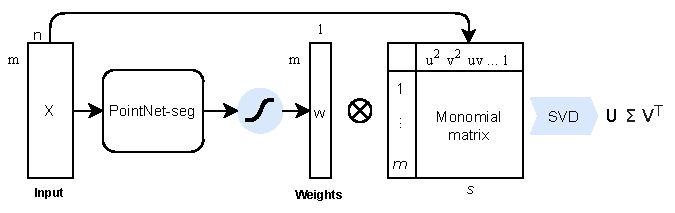
\includegraphics[width=1.0\textwidth]{consensus}
	\caption{}
	\label{fig:consensus}
\end{figure}

Because the fundamental matrix is a constraint expressed by 1 linear equation a basis of only 1  nullspace vector is needed from the singular value decomposition to construct it. But the method can also be used to learn constraints such as a homography or rigid 3D transformation that are constrained by 3 linear equations and therefore require a basis of 3 nullspace vectors. In that case the last 3 singular values from the SVD should be minimized in the loss function.

In the following sections the method used to extract the homography from the basis vectors will be explained. Two points that are related by a homography is expressed as follows. The monomials are grouped by parentheses.

\[
u \times Hv=0 \rightarrow
\]
\[
[u]_{\times} Hv=0 \rightarrow
\]
\[
\begin{pmatrix}
0 & -1 & u_y \\
1 & 0 & -u_x \\
-u_y & u_x & 0 \\
\end{pmatrix}
\begin{pmatrix}
h_{11} & h_{12} & h_{13} \\
h_{21} & h_{22} & h_{23} \\
h_{31} & h_{32} & h_{33} \\
\end{pmatrix}
\begin{pmatrix}
v_x \\
v_y \\
1 \\
\end{pmatrix}
=
\begin{pmatrix}
0 \\
0 \\
0 \\
\end{pmatrix}
\rightarrow
\]
\[
\begin{cases}
-h_{21} (v_x) \ \ \ \ - h_{22} (v_y) \ \ \ \ - h_{23} (1) \ \ \ + h_{31} (v_x u_y) + h_{32} (v_y u_y) + h_{33} (u_y) = 0 \\
\ \ h_{11} (v_x) \ \ \ \ \ + h_{12} (v_y) \ \ \ \ + h_{13} (1) \ \ -h_{31} (v_x u_x) -h_{32} (v_y u_x) - h_{33} (u_x) = 0 \\
-h_{11} (v_x u_y) -h_{12} (v_y u_y) -h_{13} (u_y) + h_{21} (v_x u_x) + h_{22} (v_y u_x) + h_{23} (u_x) = 0 \\
\end{cases}
\]

The monomials are the same as for the fundamental constraint, which means that the same Vandermonde matrix $M$ can be used. But because an homography is constrained by $r=3$ linear equations the last 3 singular values of the SVD should be minimized during training.

Extract 3 basis vectors from the nullspace which will be the 3 rightmost columns of $ V $ in the SVD of $diag(\textbf{w})M$.

\[
B = 
\begin{pmatrix}
\textbf{v}_7 & \textbf{v}_8 & \textbf{v}_9
\end{pmatrix}
\in \mathbb{R}^{9x3}
\]

The 3 linear equations of the homography are tangled which means that the elements of $B$ can not be directly mapped onto the elements in $H$. Notice that the first equation of $H$ does not contain $u_y$ and the second equation of $H$ does not contain $u_x$. We can exploit this fact to perform a change of basis from $B \in \mathbb{R}^{9x3}$ to $B' \in \mathbb{R}^{9x2}$ that should have the following structure.

\begin{center}
\begin{tabular}{ c c c }
	Monomial & Structure of $B'$ & Corresponding element in $H$ \\
	$u_x v_x$ & \multirow{9}{*}{
$\begin{pmatrix}
	0 & . \\
	0 & . \\
	0 & . \\
	. & 0 \\
	. & 0 \\
	. & 0 \\
	. & . \\
	. & . \\
	. & . \\
\end{pmatrix}$
} & \multirow{9}{*}{
$\begin{pmatrix}
 & h_{31} \\
 & h_{32} \\
 & h_{33} \\
h_{31} &   \\
h_{32} &   \\
h_{33} &   \\
h_{21} & h_{11} \\
h_{22} & h_{12} \\
h_{23} & h_{13} \\
\end{pmatrix}$
} \\
	$u_x v_y$ & \\
	$u_x \ \ \ \ $ & \\    
	\hline
	$u_y v_x$ & \\
	$u_y v_y$ & \\
	$u_y \ \ \ \ $ & \\    
	\hline
	$\ \ \ \ v_x$ & \\
	$\ \ \ \ v_y$ & \\
	$\ \ \ \ 1$ & \\
\end{tabular}
\end{center}

To perform the change of basis to get the structure of $B'$ we use the nullspace $\textbf{n}_1 \in \mathbb{R}^{3\times 1}$ of rows 1, 2 and 3 from $B$, and the nullspace $\textbf{n}_2 \in \mathbb{R}^{3x1}$ of row 4, 5, 6 from $B$.

\[
A_1 = 
\begin{pmatrix}
b_{11} & b_{12} & b_{13} \\
b_{21} & b_{22} & b_{23} \\
b_{31} & b_{32} & b_{33} \\
\end{pmatrix},
A_2 = 
\begin{pmatrix}
b_{41} & b_{42} & b_{43} \\
b_{51} & b_{52} & b_{53} \\
b_{61} & b_{62} & b_{63} \\
\end{pmatrix}
\]
\[
\textbf{n}_1 = \textit{"rightmost column of right-singular vectors of A1"}
\]
\[
\textbf{n}_2 = \textit{"rightmost column of right-singular vectors of A2"}
\]
\[
\textbf{b}^{n_1} = B\textbf{n}_1
\]
\[
\textbf{b}^{n_2} = B\textbf{n}_2
\]

Now the $\textbf{b}^{n_1}$ and $\textbf{b}^{n_2}$ basis vectors will have the following structure as desired.

\[
\textbf{b}^{n_1} =
\begin{pmatrix}
0 \\
0 \\
0 \\
. \\
. \\
. \\
. \\
. \\
. \\
\end{pmatrix},
\textbf{b}^{n_2} =
\begin{pmatrix}
. \\
. \\
. \\
0 \\
0 \\
0 \\
. \\
. \\
. \\
\end{pmatrix},
\]

The basis vectors have zeros at the correct place. The next step is to adjust the scale so that row 4, 5 and 6 of $\textbf{b}^{n_1}$ and row 1, 2 and 3 of $\textbf{b}^{n_2}$ have the same norm because they both represent the same elements $h_{31}$, $h_{32}$ and $h_{33}$. We also make sure they have the same sign.

\[
s = \sign(b^{n_2}_1 + b^{n_2}_2 + b^{n_2}_3) \sign(b^{n_1}_4 + b^{n_1}_5 + b^{n_1}_6)
\]

$s$ will be -1 if they have different signs, or 1 if they are the same sign.

\[
B'=
\begin{pmatrix}
\textbf{b}^{n_1} / \norm{(b^{n_1}_4 \ b^{n_1}_5 \ b^{n_1}_6)
} &
\textbf{b}^{n_2} / \norm{(b^{n_2}_1 \ b^{n_2}_2 \ b^{n_2}_3)} s
\end{pmatrix}
\in \mathbb{R}^{9x2}
\]

It is now possible to assign the elements of $H$ by pattern matching.

\[
H=
\begin{pmatrix}
\ \ b'_{72} & \ \ b'_{82} & \ \ b'_{92} \\
\ \ b'_{71} & \ \ b'_{81} & \ \ b'_{91} \\
-b'_{41} & -b'_{51} & -b'_{61} \\
\end{pmatrix}
\]

The method not only works for predicting the fundamental or homographic relationship between points, but can also be used for 3D rigid transformations.

\[
v=Ru+t \rightarrow
\]
\[
Ru+t-v=0 \rightarrow
\]
\[
\begin{pmatrix}
r_{11} & r_{12} & r_{13} \\
r_{21} & r_{22} & r_{23} \\
r_{31} & r_{32} & r_{33} \\
\end{pmatrix}
\begin{pmatrix}
u_x \\
u_y \\
y_z \\
\end{pmatrix}
+
\begin{pmatrix}
t_x \\
t_y \\
t_z \\
\end{pmatrix}
-
\begin{pmatrix}
v_x \\
v_y \\
v_z \\
\end{pmatrix}
=
\begin{pmatrix}
0 \\
0 \\
0 \\
\end{pmatrix}
\rightarrow
\]
\[
\begin{cases}
r_{11} (u_x) + r_{12} (u_y) + r_{13} (u_z) + t_x (1) - (v_y) = 0 \\
r_{21} (u_x) + r_{22} (u_y) + r_{23} (u_z) + t_y (1) - (v_x) = 0 \\
r_{31} (u_x) + r_{32} (u_y) + r_{33} (u_z) + t_z (1) - (v_z) = 0 \\
\end{cases}
\]

The monomials in the parentheses form the following Vandermonde matrix.

\[
M=
\begin{pmatrix}
u_{x,1} & u_{y,1} & u_{z,1} & v_{x,1} & v_{y,1} & v_{z,1} & 1 \\
 & & & \vdots & & & \\
u_{x,m} & u_{y,m} & u_{z,m} & v_{x,m} & v_{y,m} & v_{z,m} & 1 \\
\end{pmatrix}
\]

The constraint of $r=3$ linear equations is satisfied for all inliers if

\[
\diag(\textbf{w})
M
\begin{pmatrix}
r_{11} & r_{21} & r_{31} \\
r_{12} & r_{22} & r_{32} \\
r_{13} & r_{23} & r_{33} \\
-1 & 0 & 0 \\
0 & -1 & 0 \\
0 & 0 & -1 \\
t_x & t_y & t_z \\
\end{pmatrix}
=
\begin{pmatrix}
0 \\
\vdots \\
0 \\
\end{pmatrix}
^{mx1}
\]

Similar to before $R$ and $t$ is extracted from the null vectors of $\diag(\textbf{w})M$. The null vectors are the 3 rightmost singular vectors in the SVD. The 3 null vectors form a basis matrix $B$ on which a change of basis is performed to untangle the components $v_x$, $v_y$ and $v_z$ into a new structure $B'$ where $R$ and $t$ are easy to extract.

\begin{center}
	\begin{tabular}{ c c c }
		Monomial & Structure of $B'$ &  \\
		$u_x$ & \multirow{7}{*}{
			$\begin{pmatrix}
			r_{11} & r_{21} & r_{31} \\
			r_{12} & r_{22} & r_{32} \\
			r_{13} & r_{23} & r_{33} \\
			-1 & 0 & 0 \\
			0 & -1 & 0 \\
			0 & 0 & -1 \\
			t_x & t_y & t_z \\
			\end{pmatrix}$
		} \\
		$u_y$ & \\
		$u_z$ & \\    
		\hline
		$v_x$ & \\
		$v_y$ & \\
		$v_z$ & \\    
		\hline
		$1$ & \\
	\end{tabular}
\end{center}

\[
B'=
-
\begin{pmatrix}
b_{41} & b_{42} & b_{43} \\
b_{51} & b_{52} & b_{53} \\
b_{61} & b_{62} & b_{63} \\
\end{pmatrix}^{-1}
\begin{pmatrix}
b_{11} & b_{12} & b_{13} \\
b_{21} & b_{22} & b_{23} \\
b_{31} & b_{32} & b_{33} \\
b_{41} & b_{42} & b_{43} \\
b_{51} & b_{52} & b_{53} \\
b_{61} & b_{62} & b_{63} \\
b_{71} & b_{72} & b_{73} \\
\end{pmatrix}
=
\begin{pmatrix}
r_{11} & r_{21} & r_{31} \\
r_{12} & r_{22} & r_{32} \\
r_{13} & r_{23} & r_{33} \\
-1 & 0 & 0 \\
0 & -1 & 0 \\
0 & 0 & -1 \\
t_x & t_y & t_z \\
\end{pmatrix}
\]

However this holds for any affine transformation, to enforce the rotation manifold constraint an additional regularizer loss term is added.

\[
\mathcal{L}_r=\log(1 + || RR^T - I_{3\times3} ||)
\]

\subsection{Improving training convergence}

After some initial attempts at training the consensus maximization network for hagiographies on the output of the keypoint network, it was clear that it was next to impossible to get the training to converge on a good solution. Applying some additional techniques not described in the original paper resolved the issue.

Firstly the points should be transformed into a different basis before they are fed into the consensus maximization network. The change of basis ensures that the coordinates are scaled so that their maximum magnitude is 1, and the origin is centered in the middle of the image and not in the top left corner.

\[
G=
\begin{pmatrix}
W & 0 & W/2 \\
0 & W & H/2 \\
0 & 0 & 1 \\
\end{pmatrix}
\]
\[
p' = G^{-1} p
\]
Where $p$ is the output point from the keypoint network, $W$ and $H$ is the width and height of the image respectively, and $p'$ is the new altered point used as input. The homography $H$ predicted by the consensus maximization network will be in this new basis $G$ and needs to be altered in order to use it in our standard pixel coordinate basis as follows.

\[
H' = G H G^{-1}
\]

The second method to improve convergence during training is to normalize the rows of the Vandermonde matrix as follows.

\[
M_n' = \frac{M_n}{||M_n||}
\]

For all $n$ rows of the Vandermonde matrix $M$.







\iffalse

\subsection{CNN architectures}

In order to predict depth and motion from monocular images two different CNN architectures will be implemented.

\paragraph{SfMLearner} This is the architecture from \cite{sfmlearner}. The authors use a DispNet\cite{dispnet} architecture to predict depth maps at four different scales, and a ResNet18\cite{resnet} architecture with modified decoder to predict pose updates in an euler angle axis representation.

\paragraph{Monodepth2} This is the architecture from \cite{monodepth2}. The authors use a ResNet18 architecture instead of a DispNet architecture to predict depth estimates. They make this choice because its a smaller and faster architecture. Similarly they use a ResNet18 architecture with modified decoder to predict the pose updates in an euler angle axis representation.

\subsection{Differentiable depth image warping}
\label{sec:diffwarp}

Central to all previous methods in the related work section is the differentiable depth image warp operation in the loss function of the CNN networks. Given the intrinsic camera matrix:

\[
K = 
\begin{pmatrix}
f_x & s & x_0 \\
0 & f_y & y_0 \\
0 & 0   & 1
\end{pmatrix}
\]

And the predicted depth $ D_t(p_t) $ of pixel $ p_t $ of the target (current) frame. And the transform $ T_{t \rightarrow s} $ from the target to source (next/previous) frame:

\[
T_{t \rightarrow s} =
\begin{pmatrix}
\textbf{R} & \textbf{t} \\
0 & 1
\end{pmatrix}
\]

The position of the target pixel $ p_t $ in the source image $ p_s $ can be calculated in homogeneous coordinates as:

\[
p_s \sim K T_{t \rightarrow s} D_t(p_t) K^{-1} p_t 
\]

The pixel position $ p_s $ is however continuous and in order to sample the discrete source image $ I_s $ a differentiable bilinear sampling method is used. The method is described in \textit{spatial transformer networks}\cite{spatialtransformernetworks} and works by interpolating the neighbouring 4 pixels values (top-left, bottom-right) by the distance to the the continuous sampling point $ p_t $.

\subsection{Loss functions}
\label{sec:loss}

\paragraph{Photometric loss} Is defined as $ \mathcal{L}_p(I_t, \hat{I}_s)=|I_t - \hat{I}_s| $.

\paragraph{SSIM loss} Is defined as $ \mathcal{L}_{ssim}(I_t, \hat{I}_s)=\dfrac{1-\textrm{SSIM}(I_t, \hat{I}_s)}{2} $.

\paragraph{Combined loss} The photometric and SSIM loss is often combined and balanced using $ \mathcal{L}_{ps}(I_t, \hat{I}_s) = \alpha \mathcal{L}_{ssim} + (1-\alpha) \mathcal{L}_p $

\paragraph{Depth smooth loss} Is defined as $ \mathcal{L}_{smooth}(D_t)=|\delta_x^2 D_t|+|\delta_y^2 D_t| $. Not ideal because it can cause very fussy edges as seen in SfMLearner.

\paragraph{Edge aware depth smooth loss} Is defined as $ \mathcal{L}_{edge}(D_t)=|\delta_x D_t|e^{-|\delta_x I_t|} + |\delta_y D_t|e^{-|\delta_y I_t|} $. Applied in Monodepth2 giving sharper edges because the smoothness term is weighted to mostly affect areas with small photometric derivitive.

\paragraph{Velocity supervision loss} When a velocity measurement exists in the dataset a term to enforce scale accurate estimates can be added like $ \mathcal{L}_{v} = \bigr{|} \| \textbf{t}_{t \rightarrow s} \| - |v|\Delta t \bigr{|} $, as proposed in packnet\cite{packnet}.

\subsection{Handling occlusions}
\label{sec:occlusion}

\paragraph{Disparity loss} To encourage background depths (low disparities) in shadows of the depth map where occlusion has occurred a penalty on the disparity can be added $ \mathcal{L}_{o} =|d_t|. $

\paragraph{Minimum loss across frames} In SfMLearner the photometric loss is calculated for the previous and next frames compared to the current in the sequence. The pixel wise average across the frames are then used. This causes problems if a pixel is for example occluded in the previous frame, but visible in the current and next frame. In this situation the average loss will be pretty high even though a correct depth and transformation has been predicted, because of the occluded pixel. Instead Monodepth2 suggests to pick the minimum per pixel error over the frames which creates a more telling loss. 

\subsection{Handling model limitations}
\label{sec:modellimit}

In order to optimize using the photometric reprojecton error as the loss function two assumptions must hold. Firstly the scene must be static, meaning all objects in the scene must be still except the moving camera. Movement by cars and humans in the scene that is not due to the camera movement will cause problems. Secondly there must be photometric consistency between frames for the photometric error to make sense. This means that non lambertian surfaces, change in lighting, and change in exposure between frames will cause problems.

\paragraph{Explainability mask} The authors of \cite{sfmlearner} tackle this problem by having a CNN predict what pixels are valid to use in the photometric loss function. It shares the encoder of the pose predicting network but branches of into a different encoder which estimates a mask of the valid/explainable pixels. The loss function for the mask is the cross entropy loss compared to a mask filled with ones. The photometric loss function is augmented to include the explainability mask removing pixels that cannot be explained by the predicted depth and transformation. This encourages the mask to be filled with ones, but allows some slack due to pixels that can not be explained by the photometric loss.

\paragraph{Stationary pixels mask} The authors of \cite{monodepth2} introduced a mask to remove stationary pixels from the set of previous, current and next frame. This is done by creating a mask where the photometric error is smaller before applying the projection than after. This works because stationary pixels that have not moved in relation to the camera will of course have a small photometric loss without reprojection. This will remove pixels from the car dashboard and also nearby vehicles that are traveling at the same speed.

\subsection{Multi-scale estimation}

In the depth decoder 4 different scales of the depth map is created. In SfMLearner downsamples the target image to the size of the depth map when calculating the loss. The authors of Monodepth2 noticed that this creates holes in the depth prediction on some surfaces because it creates ambiguities for the pixels removed during downsampling. Their approach is instead to resize the depth map to the target image size using interpolation, which turns out to work better.

\fi
\chapter{Results}\label{cha:results}

This chapter presents the results from the experiments conducted to evaluate the performance of the unsupervised learning methods investigated in this thesis. 

\section{Depth and ego motion}

\begin{figure}[H]
	\centering
	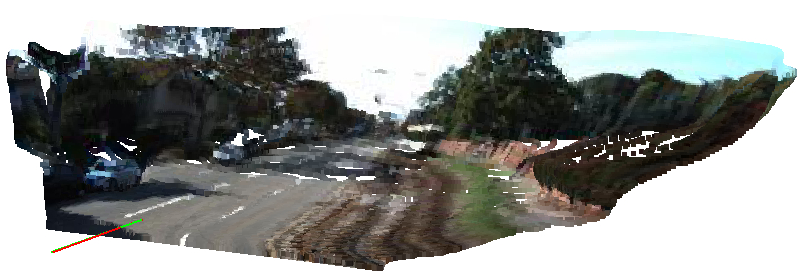
\includegraphics[width=1.0\textwidth]{3drender}
	\caption{3D render of colorized depth map}
	\label{fig:3drender}
\end{figure}

\begin{figure}[H]
	\centering
	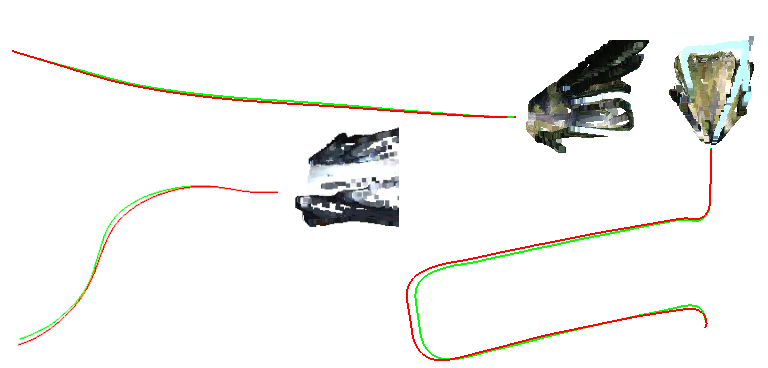
\includegraphics[width=0.8\textwidth]{motion2}
	\caption{3D visualization of the camera movement in three different image sequences. The green lines are the ground truth and the red lines are the predicted camera trajectories.}
	\label{fig:movement}
\end{figure}


\begin{table}[H]
\centering
\begin{tabular}{|l|c|c||c|c||c|c||c|c|c|c|}
\hline
C & Net & DS & Edge & Norm & Expl & Stat & SSIM & Comb & US \\
\hline
1 & SL & K &  &  &  &  &  & avg &  \\
\hline
2 & SL & K &  &  & $ \times $ &  &  & avg &  \\
\hline
3 & SL & K &  &  &  & $ \times $ &  & avg &  \\
\hline
4 & SL & K & $ \times $ &  &  & $ \times $ &  & avg &  \\
\hline
5 & SL & K & $ \times $ &  &  & $ \times $ & $ \times $ & min &  \\
\hline
6 & SL & K & $ \times $ & $ \times $ &  & $ \times $ & $ \times $ & min &  \\
\hline
7 & SL & K & $ \times $ & $ \times $ &  & $ \times $ & $ \times $ & min & $ \times $ \\
\hline
8 & SL & L & $ \times $ & $ \times $ &  & $ \times $ & $ \times $ & min & $ \times $ \\
\hline
9 & M2 & K &  &  &  & $ \times $ &  & avg &  \\
\hline
10 & M2 & K & $ \times $ & $ \times $ &  & $ \times $ & $ \times $ & min &  \\
\hline
11 & M2 & K & $ \times $ & $ \times $ &  & $ \times $ & $ \times $ & min & $ \times $ \\
\hline
12 & M2 & L & $ \times $ & $ \times $ &  & $ \times $ & $ \times $ & min & $ \times $ \\
\hline
\end{tabular}
\caption{All configurations of the depth and ego motion network that were evaluated. The C column identifies the specific configuration. The Net column shows which architecture was used, either SL for SfmLearner or M2 for Monodepth2. The DS column shows which dataset was used during training, either K for Kitti or L for Lyft. The Edge column indicates if the edge aware smoothing loss term $\mathcal{L}_{edge}$ was used. The Norm column indicates if depth map normalization was used. The Expl column indicates if an explainability mask was used. The Stat column indicates if a mask to remove stationary pixels from the loss was used. The SSIM column indicates if $\mathcal{L}_{ps}$ was used, otherwise just $\mathcal{L}_{p}$. The Comb column shows which methods was used to combine the loss terms from the two source images, either the average or the minimum loss across frames. The US column indicates that up scaling of the depth maps in the pyramid was used, otherwise the target frame was down scaled to match the size of the smaller depth maps in the pyramid.}
\label{table:configurations}
\end{table}


\begin{table}[H]
\centering
{\setlength{\tabcolsep}{0.4em}
\begin{tabular}{|r|r|c||l|l|l|l||l|l|l||l|}
\hline
E & C & DS & AbsRel & SqRel & RMSE & RMSLE & $1.25$ & $1.25^2$ & $1.25^3$ & Ego \\
\hline
1 & 1 & K & 0.174 & 1.405 & 4.829 & 0.249 & 0.784 & 0.920 & 0.964 & 0.024 \\
\hline
2 & 2 & K & 0.184 & 1.718 & 4.953 & 0.258 & 0.776 & 0.915 & 0.960 & 0.020 \\
\hline
3 & 3 & K & 0.140 & 0.793 & 4.549 & 0.217 & 0.818 & 0.939 & 0.976 & 0.020 \\
\hline
4 & 4 & K & 0.143 & 0.819 & 4.708 & 0.222 & 0.810 & 0.937 & 0.975 & 0.022 \\
\hline
5 & 5 & K & 0.133 & 0.727 & 4.305 & 0.204 & 0.843 & 0.950 & 0.979 & 0.023 \\
\hline
6 & 6 & K & 0.137 & 0.797 & 4.282 & 0.208 & 0.837 & 0.948 & 0.977 & 0.024 \\
\hline
7 & 7 & K & 0.135 & 0.778 & 4.248 & 0.208 & 0.841 & 0.948 & 0.997 & 0.020 \\
\hline
8 & 7 & L & 0.340 & 7.811 & 23.071 & 0.447 & 0.457 & 0.734 & 0.868 & 0.043 \\
\hline
9 & 8 & K & 0.512 & 5.185 & 10.757 & 0.611 & 0.305 & 0.549 & 0.732 & 0.495 \\
\hline
10 & 8 & L & 0.739 & 20.236 & 31.859 & 0.773 & 0.240 & 0.434 & 0.587 & 1.324 \\
\hline
11 & 9 & K & \textbf{0.125} & \textbf{0.697} & 4.298 & 0.203 & 0.845 & 0.948 & 0.979 & 0.021 \\
\hline
12 & 10 & K & 0.126 & 0.714 & 4.018 & \textbf{0.194} & \textbf{0.860} & \textbf{0.958} & \textbf{0.982} & \textbf{0.019} \\
\hline
13 & 11 & K & 0.132 & 0.769 & \textbf{3.966} & 0.196 & 0.859 & 0.957 & 0.981 & \textbf{0.019} \\
\hline
14 & 11 & L & 0.304 & 7.019 & 21.907 & 0.414 & 0.518 & 0.775 & 0.886 & 0.042 \\
\hline
15 & 12 & K & 0.322 & 3.177 & 7.179 & 0.378 & 0.549 & 0.797 & 0.906 & 0.036 \\
\hline
16 & 12 & L & 0.303 & 8.051 & 19.312 & 0.385 & 0.637 & 0.827 & 0.906 & 0.059 \\
\hline
\end{tabular}}
\caption{All the experiments measuring the performance of the different configurations in Table \ref{table:configurations}. The E column identifies a specific experiment. The C column shows which configuration was used. The DS column shows which Dataset was used during testing, K for Kitti and L for Lyft. The dataset used during testing differs from the one used during training in some experiments. The AbsRel, SqRel, RMSE and RMSLE columns are the depth error metrics described in section \ref{sec:depthmetrics}, smaller is better. The $1.25$, $1.25^2$ and $1.25^3$ columns are the depth accuracy metrics described in section \ref{sec:depthmetrics}, larger is better. The Ego column is the camera ego motion error metric described in section \ref{sec:egometric}.}
\label{table:experiments}
\end{table}

TODO: Describe the improvements (if any) seen by applying each additional method for depth prediction and explain why this could be....

\iffalse
\begin{figure}[H]
	\centering
	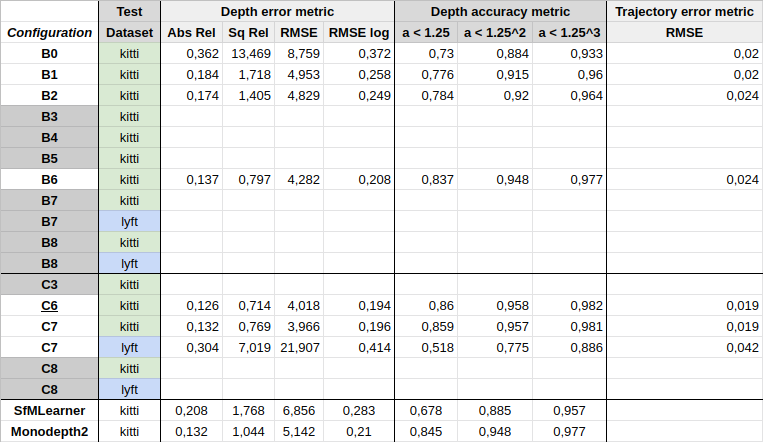
\includegraphics[width=1.0\textwidth]{evaluation}
	\caption{Evaluation metrics when testing the configurations on the testing split of the datasets}
	\label{fig:evaluation}
\end{figure}
\fi

\clearpage

\begin{figure}[H]
	\centering
	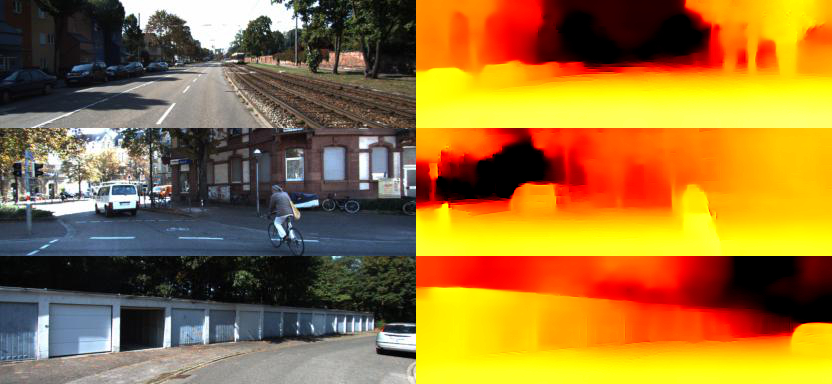
\includegraphics[width=1.0\textwidth]{depthmaps}
	\caption{Examples from the Kitti dataset}
	\label{fig:depthmapskitty}
\end{figure}

\begin{figure}[H]
	\centering
	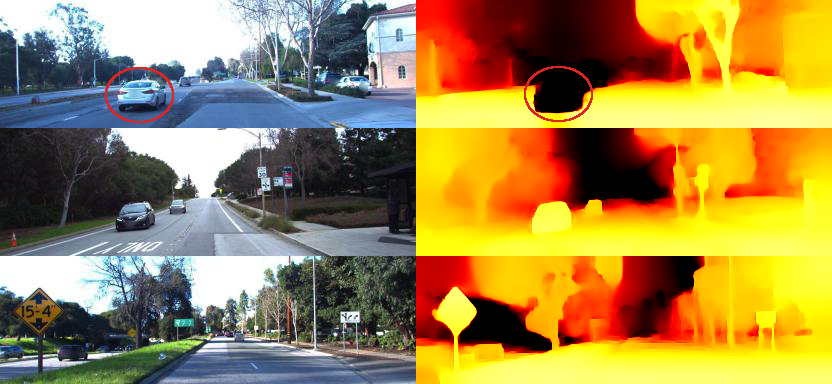
\includegraphics[width=1.0\textwidth]{depthmapslyft}
	\caption{Examples from the Lyft dataset}
	\label{fig:depthmaplyft}
\end{figure}

\begin{figure}[H]
	\centering
	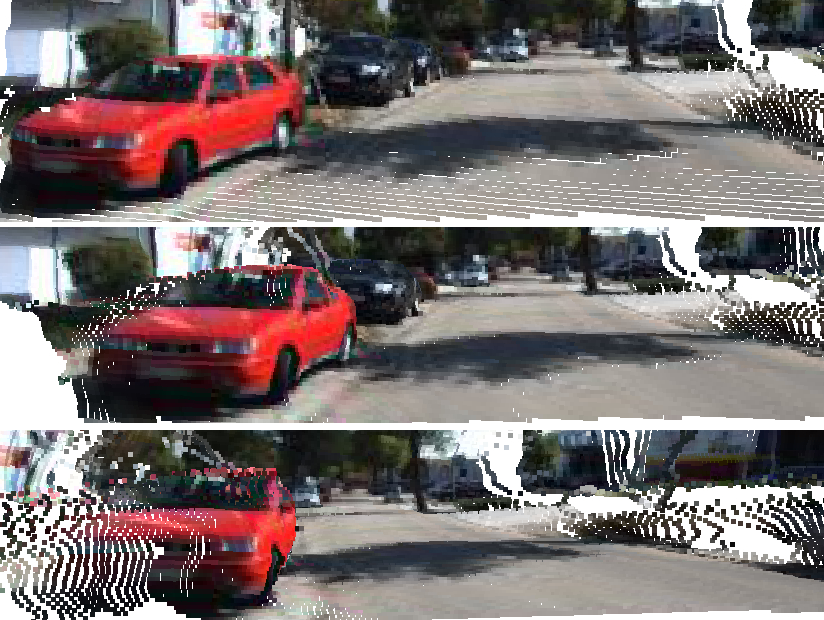
\includegraphics[width=0.8\textwidth]{3dseq}
	\caption{3D visualization from 3 different angles of the same frame in the kitti dataset.}
	\label{fig:3dseq}
\end{figure}

\section{Keypoint detection}

\begin{figure}[H]
	\centering
	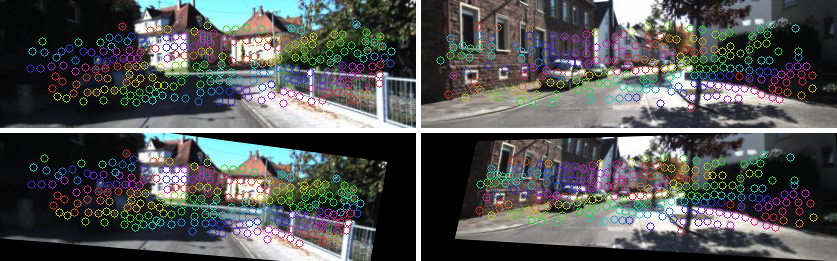
\includegraphics[width=1.0\textwidth]{point1}
	\caption{Results from the keypoint prediction network. The top row are the original input images fed to branch A, and bellow are the transformed images fed to branch B. Circles that are the same color have matching descriptors.}
	\label{fig:point1}
\end{figure}

\begin{table}[H]
\centering
\begin{tabular}{|l|l|l|l|l|l|l|}
\hline
Method & RS $\uparrow$ & LE $\downarrow$ & MS $\uparrow$ & CMR $\uparrow$ & Nt & Nm \\
\hline
UnsuperPoint & 0.796 & \textbf{0.666} & \textbf{0.488} & \textbf{0.834} & 338 & 203 \\
ORB & \textbf{0.841} & 0.764 & 0.302 & 0.564 & 310 & 171 \\
\hline
\end{tabular}
\caption{Experiments measuring the performance of keypoint detection methods.}
\label{table:pointsbenchmark}
\end{table}

TODO: Describe what the results are showing....

\section{Consensus maximization}

\begin{figure}[H]
	\centering
	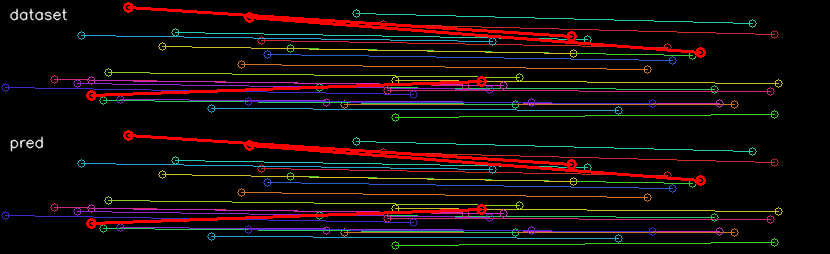
\includegraphics[width=1.0\textwidth]{synthhomo}
	\caption{Outlier detection in homography estimation in synthetic dataset. Top row is ground truth and bottom row is the prediction.}
	\label{fig:synthhomo}
\end{figure}

\begin{figure}[H]
	\centering
	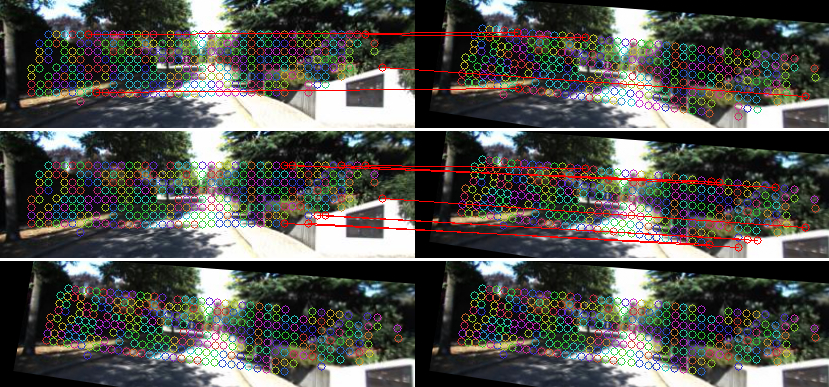
\includegraphics[width=1.0\textwidth]{kittihomo}
	\caption{Outlier detection and homography estimation on images from kitti dataset. First row is from OpenCV findHomography(), second row is from the network, third row is the image from branch A transformed by the homographgy found by OpenCV, fourth row is the image from branch A transformed by the homography found by the network.}
	\label{fig:kittihomo}
\end{figure}

\begin{table}[H]
	\centering
	\begin{tabular}{|l|l|l|l|}
		\hline
		Method & HE $\downarrow$ \\
		\hline
		ConsensusNet & ??? \\
		RANSAC & ??? \\
		\hline
	\end{tabular}
	\caption{Metrics for homography estimation.}
	\label{table:pointsbenchmark}
\end{table}

\begin{table}[H]
\centering
\begin{tabular}{l|l|c|c|c}
	\multicolumn{2}{c}{}&\multicolumn{2}{c}{Predicted}&\\
	\cline{3-4}
	\multicolumn{2}{c|}{}&Inlier&Outlier&\multicolumn{1}{c}{Total}\\
	\cline{2-4}
	\multirow{2}{*}{Actual}& Inlier & $TP$ & $FN$ & $TP+FN$\\
	\cline{2-4}
	& Outlier & $FP$ & $TN$ & $FP+TN$\\
	\cline{2-4}
	\multicolumn{1}{c}{} & \multicolumn{1}{c}{Total} & \multicolumn{1}{c}{$TP+FP$} & \multicolumn{    1}{c}{$FN+TN$} & \multicolumn{1}{c}{$N$}\\
\end{tabular}
	\caption{Confusion matrix for inlier/outlier prediction using ConsensusNet.}
	\label{table:consensusconfusion}
\end{table}


\begin{table}[H]
	\centering
	\begin{tabular}{l|l|c|c|c}
		\multicolumn{2}{c}{}&\multicolumn{2}{c}{Predicted}&\\
		\cline{3-4}
		\multicolumn{2}{c|}{}&Inlier&Outlier&\multicolumn{1}{c}{Total}\\
		\cline{2-4}
		\multirow{2}{*}{Actual}& Inlier & $TP$ & $FN$ & $TP+FN$\\
		\cline{2-4}
		& Outlier & $FP$ & $TN$ & $FP+TN$\\
		\cline{2-4}
		\multicolumn{1}{c}{} & \multicolumn{1}{c}{Total} & \multicolumn{1}{c}{$TP+FP$} & \multicolumn{    1}{c}{$FN+TN$} & \multicolumn{1}{c}{$N$}\\
	\end{tabular}
	\caption{Confusion matrix for inlier/outlier prediction using RANSAC.}
	\label{table:consensusconfusion}
\end{table}

TODO: Insert actual numbers from the testing code and describe what the results are showing....
\chapter{Discussion}\label{cha:discussion}

The best combination for depth and ego motion predictions.

Small disparity, large depth, for cars moving with the same relative speed, no ego motion.

Over-fitting while training homography.

Alterations needed to make consensus converge.

Future work to couple the training of depth, keypoints and consensus more tightly.
\section{Conclusions}

The goal of this thesis has been to evaluate a few different unsupervised learning methods in the context of structure from motion. The techniques were combined in new ways and trained on new datasets not used in previous work.

\paragraph{\textbf{How well do the unsupervised methods from previous research work on new datasets not tested in the original papers?}} As we have seen, the depth prediction networks can learn to predict depth on the Lyft dataset, not used in previous work. The keypoint prediction network can be trained on images from the Kitti dataset. With some alterations to the consensus maximization network, to improve convergence, it can be trained on the output of the keypoint prediction network. This gives us more confidence that the 3 systems could be chained together and trained jointly in future work. The performance of each technique is detailed in the results chapter.

\paragraph{\textbf{What are the performance gains of combining different methods from recent research in monocular depth and ego motion prediction?}} Table \ref{table:experiments} lists all experiments conducted to compare different techniques in monocular depth and ego motion prediction. The biggest performance gains comes from using SSIM in the photometric error, and using the min() function to combine the per pixel loss across frames. Using a stationary pixel mask seems to be more effective compared to using a predicted explainability mask. Using the edge aware depth smoothess loss term does not improve the metrics much, but does give sharper depth maps upon visual inspection. The techniques with the least impact are depth map normalization and depth map upscaling.
\\
\\
We conclude that the goal of the project has been reached, and that there is a big potential in further research into this field.

\clearemptydoublepage
\backmatter

\bibliography{IEEEfull,myrefs}

\printindex

\end{document}
